\documentclass[doctor]{USTBThesis}

% \usepackage{multirow}
% \usepackage[inner=0.75in,outer=0.65in,top=0.75in,bottom=0.75in]{geometry}
% \usepackage{mathpazo}
\raggedbottom
\begin{document}

\CTEXsetup[number={\arabic{chapter}}]{chapter}
\CTEXsetup[name={,}]{chapter}
\CTEXsetup[nameformat={\zihao{-3} \bfseries }]{chapter}
\CTEXsetup[titleformat={\zihao{-3} \bfseries }]{chapter}
\floatname{algorithm}{算法}

\newcommand{\tabref}[1]{表\ref{#1}}
\newcommand{\equref}[1]{式(\ref{#1})}
\newcommand{\secref}[1]{\ref{#1}节}
\renewcommand{\algref}[1]{算法\ref{#1}}

% \usepackage{enumitem}
\setenumerate[1]{itemsep=0pt,partopsep=0pt,parsep=\parskip,topsep=5pt}
\setitemize[1]{itemsep=0pt,partopsep=0pt,parsep=\parskip,topsep=5pt}
\setdescription{itemsep=0pt,partopsep=0pt,parsep=\parskip,topsep=5pt}


%论文信息
% !Mode:: "TeX:UTF-8"

%学校名称
\university{北京科技大学}{University of Science and Technology Beijing}

%学院
\school{计算机与通信工程学院}{School of Computer and Communication Engineering}

%专业
\major{计算机科学与技术}{Computer Science and Technology}

%论文题目,前两个是主标题中英文,后两个是副标题中英文
\thesistitle{基于深度微分方程网络的复杂动态系统建模与控制}{Modeling and Controlling for Complicated Dynamical System based on Deep Differential Equation Network}{基于深度微分方程网络的复杂动态系统建模与控制}{Modeling and Controlling for Complicated Dynamical System based on Deep Differential Equation network}

%作者
\thesisauthor{袁兆麟}{Zhaolin Yuan}

%学号
\authorid{B20170324}

% 指导老师,第三个为指导老师单位
\teacher{班晓娟}{Xiaojuan Ban}{北京科技大学}{教授}

% 副指导老师,第三个为副指导老师单位
\subteacher{李宁}{Ning Li}{北京信息科技大学}{教授}

% 分类号
\category{TP312}

%论文提交日期
\thesisdate{2022}{10}{20}


%论文封面
% !Mode:: "TeX:UTF-8"

%论文封面
\newcommand{\makecover}{%
    % 第一封面
    \pagestyle{empty}
    ~
    \vspace{5em}

    \begin{tabular}[H]{p{60pt} p{1em}}
    % & \linespread{0.8}\selectfont \zihao{3} \heiti \textbf{\ThesisTitleCN} \\	%带英文会出现格式错误
    & \linespread{0.8}\selectfont \zihao{3} \textbf{\ThesisTitleCN} \\	%带英文会出现格式错误
    &\\
    &\linespread{0.8}\selectfont \zihao{3}  \textbf{\AuthorCN} \\
    &\\
    &\linespread{0.8}\selectfont \zihao{3}  \textbf{北京科技大学}
    \end{tabular}

    \newpage


    %第二封面
    \pagestyle{empty}
    \begin{titlepage}
        \begin{flushright}
            \hfill
            \newlength{\Mycode}
            \settowidth{\Mycode}{\textbf{密 \quad 级:}\uline{\zihao{5} \quad 公 开 \quad}}

            \begin{minipage}[t]{\Mycode}
            \textbf{密 \quad 级:}\uline{\zihao{5} \quad 公 开 \quad}
            \end{minipage}
        \end{flushright}

        \begin{center}
            \vspace{130mm}

            %论文主标题
            % \centerline{\zihao{-3} 论文题目:\zihao{-2} \textbf{\ThesisTitleCN}} \par    %强制只使用一行
            \zihao{-3} 论文题目:\zihao{-2} {\textbf{\ThesisTitleCN}} \par     %可以分行
            \vspace{10mm}

            %论文副标题,没用请注释掉
            % \centerline{\zihao{-2} —— \textbf{\ThesisSubTitleCN}} \par
            \vspace{30mm}

            \zihao{-3}

            \begin{tabular}{rc}
            学 \qquad 号:& \underline{\makebox[5cm]{\zihao{-3} \StudentID}} \\
            作 \qquad 者:& \underline{\makebox[5cm]{\zihao{-3} \AuthorCN}}\\
            专业名称:& \underline{\makebox[5cm]{\zihao{-3} \MajorCN}}
            \end{tabular}
            \vspace{10mm}

            \zihao{-3}\ThesisYear 年 \zihao{-3}\ThesisMonth 月 \zihao{-3}\ThesisDay 日

        \end{center}
    \end{titlepage}
    \newpage

    %第三封面
    \pagestyle{empty}
    \begin{titlepage}
        \begin{center}
            \qquad
            \vspace{10mm}

            \zihao{-2}
            %论文中文主标题
            % \centerline{\ThesisTitleCN} \par    %强制只使用一行
            \ThesisTitleCN \par     %可以分行
            \vspace{10mm}

            % %论文中文副标题,没用请注释掉
            % \centerline{\ThesisSubTitleCN} \par
            \vspace{20mm}

            %论文英文主标题
            % \centerline{\ThesisTitleEN} \par    %强制只使用一行
            \ThesisTitleEN \par     %可以分行
            \vspace{10mm}

            % %论文英文副标题,没用请注释掉
            % \centerline{\ThesisSubTitleEN} \par
            \vspace{40mm}

            \zihao{-4}
            研究生姓名:\AuthorCN \par
            \vspace{3mm}
            指导教师姓名:\TeacherCN \par
            \vspace{3mm}
            \UniversityCN \SchoolCN \par
            \vspace{3mm}
            北京 100083,中国 \par
            \vspace{8mm}

            Doctor Degree Candidate:\AuthorEN \par
            \vspace{3mm}
            Supervisor:\TeacherEN \par
            \vspace{3mm}
            \SchoolEN \par
            \vspace{3mm}
            \UniversityEN \par
            \vspace{3mm}
            30 Xueyuan Road, Haidian District \par
            \vspace{3mm}
            Beijing 100083, P.R.CHINA

        \end{center}
    \end{titlepage}

    \newpage

    %论文第四封面
    \pagestyle{empty}
    \begin{titlepage}
        \begin{center}
            \begin{tabular}{rccrc}
                \zihao{-4} 分类号:& \zihao{5} \underline{\makebox[2cm]{\ThesisCategory}} & \qquad \qquad &\zihao{-4} 密 \quad \space \space 级: & \zihao{5} \underline{\makebox[2cm]{公开}} \\
                \vspace{5mm}
                \zihao{-4}U D C:& \zihao{5} \underline{\makebox[2cm]{}} & \qquad \qquad & \zihao{-4} 单位代码: & \zihao{5} \underline{\makebox[2cm]{10008}}
                \end{tabular}
                \par
                \vspace{30mm}

                \zihao{-2} \textbf{北京科技大学\degreecn 学位论文} \par
                \vspace{30mm}

                \zihao{4}
                %论文主标题
                % \centerline{ \textbf{论文题目:} \underline{\makebox[10cm]{\ThesisTitleCN}} } \par    %强制只使用一行
                % \textbf{论文题目:}\underline{\makebox[10cm]{\zihao{4} \ThesisTitleCN}} \par     %可以分行
                \textbf{论文题目:} \underline{\ThesisTitleCN} \par     %可以分行

                \vspace{5mm}
                %论文副标题,没用请注释掉
                % \centerline{ —— \ThesisSubTitleCN} \par
                % \vspace{10mm}

                \centerline{ \textbf{作者:} \underline{\makebox[3cm]{\AuthorCN}} } \par
                \vspace{70mm}

                \begin{tabular}{rcrl}
                \makebox[7em][s]{\textbf{指\hspace{\fill}导\hspace{\fill}教\hspace{\fill}师:}} & \zihao{5} \underline{\makebox[3cm]{\TeacherCN \qquad \TeacherJobtitle}} & \zihao{4} \textbf{单位:} & \zihao{5} \underline{\makebox[3cm]{\TeacherDepartment}} \\
                \zihao{4} \makebox[7em][s]{\textbf{指导小组成员:}} & \zihao{5} \underline{\makebox[3cm]{\SubTeacherCN \qquad \SubTeacherJobtitle}} & \zihao{4} \textbf{单位:} & \zihao{5} \underline{\makebox[3cm]{\SubTeacherDepartment}} \\
                % \zihao{4} \makebox[7em][s]{\textbf{ }} & \zihao{5} \underline{\makebox[3cm]{\SubTeacherCN \qquad \SubTeacherJobtitle}} & \zihao{4} \textbf{单位:} & \zihao{5} \underline{\makebox[3cm]{\SubTeacherDepartment}} \\
                \zihao{4} \makebox[7em][s]{\textbf{论文提交日期:}} & \multicolumn{3}{l}{\makebox[7em][s]{\ThesisYear 年 \ThesisMonth 月 \ThesisDay 日}} \\
                \makebox[7em][s]{\textbf{学位授予单位:}} & \multicolumn{3}{l}{\makebox[7em][s]{\textbf{北\hspace{\fill}京\hspace{\fill}科\hspace{\fill}技\hspace{\fill}大\hspace{\fill}学}}}
            \end{tabular}
        \end{center}
    \end{titlepage}

    \newpage
    \pagestyle{empty}
    \quad
}

\makecover


\pagenumbering{Roman}
\setcounter{page}{1}

\fancypagestyle{plain}{
  \pagestyle{fancy}
}
\fancyhead{}
\fancyhead[CO]{\zihao{5}北京科技大学博士中期报告}
\fancyhead[CE]{\zihao{5} \ThesisTitleCN}

%致谢
% !Mode:: "TeX:UTF-8"

\chapter*{\centering  致 \space 谢}
\addcontentsline{toc}{chapter}{致谢}
在北京科技大学攻读博士的五年半对我来说意义深远。在这个过程中,我积累了知识、锻炼了心性、磨练了意志,知道了如何与人合作,明白了如何作为一个平凡的人参与伟大的事业。而我所获得的一切离不开老师、朋友、家人对我的帮助与支持。值此论文完成之际,对所有帮助过我的人表示感谢。

首先,最需要感谢的人是我的导师班晓娟教授。班老师除了在专业知识以及科研方法上提供了充足的指导外,
为我创造了得天独厚的研究环境以及高自由度的发展空间,让我能够倚着自己的兴趣和好奇心探索科学的边界。另外班老师的那句“读博士,不光是写几篇论文,而是全方位的锻炼与培养”更是我读博期间始终铭记于心的教诲,我也因此受益良多。

同样要感谢的是香港浸会大学的戴弘宁教授、挪威科技大学的王浩教授、吴狄教授、北京信息科技大学李宁教授、以及Miratlas SAS的王也弯老师。他们待我如同自己的亲学生,我在学术道路上的成长离不开各位老师不遗余力的帮助与指导。

还要感谢人工智能与三维可视化实验室的各位老师和同学。感谢姚超老师在研究方案设计、论文写作、毕业论文选题等方面提供的全方位指导。感谢张雅澜、马博渊、刘斯诺等师兄师姐给我树立了优秀的标杆指引我前进,并在我毕业、择业之际分享了宝贵的经验。同时感谢曹宇宁、何润姿、胡金龙、刘婷、李佳、周佳城、李潇睿、韩方圆、张子轩等一起参与过采矿充填项目的各位同学、师弟师妹们,跟你们一起去非洲出差、一起讨论项目实施方案、一起通宵达旦赶项目进度,是我永生难忘的日子。感谢实验室所有的老师同学,与你们交流、讨论让我学到无数宝贵的知识,因为你们让我在实验室的6年时间变得丰富多彩。

同时要感谢卢东旭、苏日娜、秦运慧、郑远硕四位博士,
% 与你们近一年来的陪伴与鼓励,与你们一起日子让我远离孤单,倍感温馨与快乐。
一年多来与你们在一起交流、吃饭、娱乐,让我远离孤单,真切地感受到了友情带给人的温馨与快乐。

最后还要感谢我的父母给我无条件的支持与关爱,让我没有任何后顾之忧地追求自己的学业。你们在我获得成就时陪伴我一起喝彩,在我最困难的时期作为我最坚实的后盾,我爱你们。

感谢非洲矿业有限公司沈家华、肖金林、姚松、王京伟等同仁在数据采集、算法测试期间提供的帮助。

感谢各位评审老师的认真评阅以及所提出的宝贵意见。

本论文承蒙国家重点研发计划项目(No.2019YFC0605300)资助,特此致谢。





%摘要
% !Mode:: "TeX:UTF-8"

%中文摘要
\chapter*{ 摘 \space 要 }
\addcontentsline{toc}{chapter}{摘要}

% 在采矿、化工、能源为代表的过程工业领域中,复杂设备或系统的运行过程具有非线性、不完全观测、高时滞等特性,
采矿、化工、能源等过程工业领域中存在诸多具有非线性、高随机、长时滞、不完全观测特性的复杂动态系统。
% ,因其存在非线性、高随机、长时滞、不完全观测等特性,
% 过程工业领域中的复杂设备或系统
% 具有非线性、高随机、长时滞等特性,
依赖于机理分析的传统动态系统辨识方法难以充分拟合系统的高复杂性。
% 数据驱动的建模方法缺少系统机理和先验知识的限制,使得训练数据需求量大,在不同场景下的泛化能力差。
依靠大量训练数据驱动的参数化建模方法难以引入系统机理和先验知识,使得训练模型所需的数据量大,且模型在不同场景下泛化能力差。
系统的高复杂性与现有建模方法的局限性造成了\textbf{系统机理难分析、动态方程难辨识、关键指标难控制}等问题。
本文围绕连续时间域下复杂动态系统建模与优化这一问题展开讨论,重点研究了连续时间系统与深度学习的结合体——\text{深度微分方程网络}在复杂系统辨识与控制优化中的应用,所提出的模型及算法有效应用于膏体充填场景下的设备数据分析与管控过程中。
具体地,本文的主要研究工作包括:

1)针对具有非线性、长时延特性且本质上为连续时间过程的复杂工业系统,本文提出一种以ODE-Net作为骨架结构的深度连续时间系统辨识模型,模型能够从连续时间域角度学习工业系统输出的自回归变化和输入对输出的长时滞、非线性影响。经过膏体浓密机系统运行数据的验证,该模型在长时预测和短时预测场景下均获得较好效果。   

2)针对不确定性动态系统在非均匀采样设定下的系统辨识问题,
本文提出了常微分方程循环状态空间模型。该模型在基础循环神经网络的状态转移中引入随机路径以建模系统的不确定性。同时,利用常微分方程网络建模相邻采样时间点之间的隐变量连续时间演化以支持非均匀采样设定下的模型训练。
另外,本文提出了一种求解批常微分方程的再参数化方法以解决时间间隔不均匀时微分方程难以并行求解、模型难以并行训练的问题。
% 另外,本文针对时间间隔不均匀情况下,批常微分方程难以并行求解的问题,提出了一种状态导数的再参数化方法,通过一致化批ODE的积分区间,实现微分方程的并行求解与训练
% 以解决批数据中时间间隔不均匀导致难以并行求解的问题。
利用膏体浓密机系统数据集和两个公有系统辨识数据集对模型进行验证,结果表明该模型在数据集存在不确定性以及稀疏非均匀采样间隔时,能获得相比基线模型更好的建模效果。

3)针对复杂工业系统动态机理未知、难以控制优化问题,本文提出了基于连续时间有模型强化学习的启发式评价网络值迭代算法。该算法采用常微分方程网络构建动态系统的预测模型,并基于积分强化学习构建控制策略的自适应评价函数。
同时,依托于评价模块与模型网络的评价、预测能力,采用随机梯度下降法生成控制指令,使得整套控制模型支持高效的在线控制与参数更新。经过尾矿浓缩机仿真模型验证,该方法在非均匀数据采样下能够获得比其他控制算法更优的控制性能。同时,该算法成功部署应用于真实矿场的膏体浓密机控制系统中,相比原始的基于固定规则的控制策略获得了更好的浓度控制效果。

4)针对具有周期多阶段特性的动态系统辨识问题,本文提出了连续时间自跳变常微分方程网络。
% 以学习连续时间周期跳变过程。
在给定序列输入输出数据的所属阶段标注下,
该模型能够从非均匀采样数据中独立学习不同阶段下的系统动态特性。同时,模型引入阶段转换预测器以学习连续时间跳变系统的阶段转移过程,进而在模型开环预测时实现内部阶段变量的自转移。实验环节利用膏体制备过程中的水泥添加系统数据对模型进行验证,
结果表明模型能够在给定系统受控输入下,准确地预测阶段间的转移时间点以及各阶段内的系统输出,基于仿真结果成功优化膏体制备过程的水泥成本及设备开关机损耗成本8.2\%。

% \vspace{-20pt}

\vskip 30bp
{

    % 在关键词冒号后添加你的关键词,使用全角逗号分割
    \textbf{ \heiti \zihao{-4} 关键词:动态系统建模 ,系统辨识,常微分方程网络,有模型强化学习,浓密机,膏体充填}
}


%英文摘要

\chapter*{ Abstract }
\addcontentsline{toc}{chapter}{Abstract}
% Based on the \LaTeX manual and referred to USTB word model for \degreeen, I
% 过程工业领域中的复杂设备或系统具有非线性、高随机、长时滞等特性,
% 进而造成系统机理难分析、动态方程难辨识,关键指标难控制等问题。
In the process industry, most complex equipments or systems have strong non-linearity, high stochasticity, and long time delay.
% his causes problems such as difficult analysis of system mechanism, difficult identification of dynamic equations, and difficult control of key indicators.
These properties lead to the difficulties in analyzing system mechanisms, identifying dynamical equations, and controling critical operational indices. 
Mechanistic-based dynamic system identification methods are weak to sufficiently fit the complexity of the system.
% Deep learning methods ignore the limitations from systematic mechanisms and prior knowledge, 
% which makes the training data requirement high and reduces generalization ability in different scenarios poor.
which raises the required size of training data and reduces the generalization in different scenarios.
% 本文围绕连续时间域下复杂动态系统的建模与优化这一问题展开讨论,重点研究了连续时间系统与深度学习的结合体——\text{深度微分方程网络}在复杂系统辨识与控制优化中的应用。
% This paper discusses the problems of modeling and control in complex dynamic systems in the continuous-time domain.
From the continuous-time domain, this paper focuses on the application of \text{deep differential equation networks}, a combination of continuous time systems and deep learning, in the identification and control optimization of complex systems.

% 针对具有非线性、长时延特性且本质上为连续时间过程的复杂工业系统,本文提出一种以ODE-net作为骨架结构的深度连续时间系统辨识模型,模型能够从连续时间域角度学习工业系统输出的自回归变化和输入对输出的非线性影响。通过真实工业数据进行验证,该模型在长时预测和短时预测场景下均获得较好效果。   
(1) For modeling non-linear and long-delayed complex industrial systems which are essentially continuous-time processes, this paper proposes a continuous-time deep system identification model based on the ODE-net backbone.
The model learns the auto-regressive changes of industrial system outputs and the non-linear and time-delayed effects from inputs on outputs in continuous-time domain. 
The evaluation conducted on real industrial dataset of paste thickener indicates that the model achieves comparable performances on both long-time prediction and short-time prediction.   

% 针对具有周期多阶段转移特性的复杂系统建模问题,本文提出了一种连续时间跳变常微分方程网络以学习连续时间周期跳变过程。
% 模型能够从非均匀采样数据中独立学习不同阶段下的系统动态特性。同时模型引入阶段转换预测器以实现开环预测时的阶段自转移。利用某工业制冷系统数据对模型进行验证,该模型能够准确地预测系统输出量以及阶段转移时间点,并辅助优化制冷系统的运行能耗。


% 针对具有随机非确定性的复杂系统建模建模问题,
% 本文提出了常微分方程循环状态空间模型。该模型在状态转移中引入随机路径以建模系统的随机非确定性,同时利用常微分方程网络建模相邻采样时间点之间的隐变量连续时间演化以支持从非均匀采样数据进行学习。
% 另外,本文提出了一种常微分方程的再参数化方法以解决批中时间间隔不均匀导致难以并行求解的问题,达到加速训练的目的。
% 结果表明该模型在稀疏非均采样以及数据集存在随机非确定性情况,能获得相比基线模型更好的预测效果。
(2) For modeling the complex systems with uncertainty, this paper proposes the  Ordinary Differential Equation Recurrent State Space Model. 
On the basis of Recurrent Neural Network, an additional stochastic path defined by latent variable is embedded in the state transition for modeling uncertainty.
Furthermore, ODE-RSSM incorporates an ordinary differential equation network to model the continuous-time evolution of latent states between adjacent time points.
Inspired from the equivalent linear transformation on integration limits,
this paper also propose an efficient reparameterization method for solving batched ODEs with non-uniform time spans in parallel for efficiently training the ODE-RSSM with irregularly sampled sequences.
% We also conduct extensive experiments to evaluate the proposed ODE-RSSM and the baselines on three input-output datasets, one of which is a rollout of a private industrial dataset with strong long-term delay and uncertainty.
Extensive experiments on three datasets, including the paste thickening dataset and two public system identification datasets, demonstrate that the ODE-RSSM outperforms other baselines in predicting uncertain system in open loop when the time spans of predicted points are uneven.

% 针对复杂工业系统控制优化问题,本文提出了一种基于有模型强化学习的启发式评价网络值迭代算法。该方法采用微分方程网络构建系统的预测模型,并采用积分强化学习构建在线控制策略及自适应评价函数。经过尾矿浓缩机仿真模型验证,该方法在非均匀数据采样下能够获得比其他控制算法更优的控制性能,且该算法成功部署应用于某矿场的浓密机控制系统中,获得了较好的浓度控制效果。
% 3)针对复杂工业系统动态机理未知、难以控制优化问题,本文提出了一种基于连续时间有模型强化学习的启发式评价网络值迭代算法。该算法采用常微分方程网络构建动态系统的预测模型,并基于积分强化学习构建控制策略的自适应评价函数。
% 同时,依托于评价模块与模型网络的评价、预测能力,采用随机梯度下降法生成控制指令。整套控制模型支持高效的在线控制与参数更新。经过尾矿浓缩机仿真模型验证,该方法在非均匀数据采样下能够获得比其他控制算法更优的控制性能。同时,该算法成功部署应用于真实矿场的膏体浓密机控制系统中,相比原始的基于固定规则的控制策略获得了更好的浓度控制效果。

(3) For controling complex industrial systems without prior knowledge of mechanism, this paper proposes a novel
continuous-time model-based reinforcement learning control algorithm, heuristic critic network value iteration (HCNVI).
% Inspired by the traditional heuristic
% dynamic programming (Heuristic dynamic programming, HDP) algorithm.
The method models the dynamical system with differential equation neural network and introduces the integral reinforcement learning to approximate the adaptive critic function under control law.
Depending on the evaluation of critic network and the prediction of model network, the controlling action is determined by stochastic gradient descent algorithms.
Experiments conducted on thickening simulation system verify that the proposed HCNVI outperforms the other control algorithms.
In the meanwhile, the method is also deployed in a thickening control system of a real paste backfilling station.
In comparison to the original rules-based controlling strategy, the algorithm is effective to control the underflow concentration in a stable range.

  

% 4)针对具有周期多阶段特性的复杂动态系统辨识问题,本文提出了连续时间自跳变常微分方程网络。
% % 以学习连续时间周期跳变过程。
% 在给定序列输入输出数据的所属阶段标注下,
% 该模型能够从非均匀采样数据中独立学习不同阶段下的系统动态特性。同时,模型引入阶段转换预测器以学习连续时间跳变系统的阶段转移过程,进而在模型开环预测时实现内部阶段变量的自转移。实验环节利用膏体制备过程中的水泥添加系统数据对模型进行验证,
% 结果表明模型能够在给定系统受控输入下,准确地预测阶段间的转移时间点以及各阶段内的系统输出,基于仿真结果成功优化膏体制备成本8.2\%。
(4) To address the problem of modeling periodic multi-staged system, this paper proposes continuous-time autonomous jump ordinary differential equation (AJ-ODE-Net) to learn continuous-time period jump systems.
% Given sequential inputs and outputs dataset whose stages variables are labeled in advanced.
Given sequential inputs and outputs belonged to labeled stages,
the model is able to independently learn the sub-dynamics in different stages from non-uniform sampled data. 
The model also introduces a stage transition predictor to realize the autonomous stage transformation in open-loop prediction. 
By evaluating the model with dataset from an cement  addition system in paste production, the results indicates the AJ-ODE-Net is accurate enough to predict the system outputs and the duration time in each stage.
The open-loop prediction of paste system runtime also assists in optimizing 8.2\% cost of backfilling.

% the training phase of critic network. 
% The results show that the
% proposed method can maintain the concentration of underflow in a
% stable horizon and performs better than other algorithms in accuracy
% and time consuming.

\vskip 30bp
{
    \zihao{-4}
    % 在key words冒号后添加你的关键词,使用半角逗号加空格分割
    $\mathbf{Key}$ $\mathbf{Words}$: 
    $\mathbf{Dynamical\ system\ modeling}$, 
    $\mathbf{Model}$-$\mathbf{based\ reinforcement}$
    $\mathbf{learning}$,
    $\mathbf{System\ identification}$, 
    $\mathbf{Ordinary\ Differential\ Equation\ Neural\ Network}$,
    $\mathbf{Thickener}$,
    $\mathbf{Paste\ backfilling}$
    
}

    % \textbf{ \heiti \zihao{-4} 关键词:动态系统建模 ,系统辨识,常微分方程网络,有模型强化学习}


% %序
% % !Mode:: "TeX:UTF-8"
%序
\chapter*{序 \space 言 }
\addcontentsline{toc}{chapter}{序言}

由于北京科技大学的论文模板在\LaTeX 方面存在空白,因此此项目具有重大的意义。



%目录
\tableofcontents

%表格目录,如果不使用请注释掉
\renewcommand{\listtablename}{\centering 表格清单}
\addcontentsline{toc}{chapter}{表格清单}
\listoftables

%图像目录,如果不使用请注释掉
\renewcommand{\listfigurename}{\centering 插图清单}
\addcontentsline{toc}{chapter}{插图清单}
\listoffigures

\pagestyle{fancy}
\fancyhead{}
\fancyhead[CO]{\zihao{5}北京科技大学\degreecn 学位论文}
\fancyhead[CE]{\zihao{5} \ThesisTitleCN}

% 第一章
% !Mode:: "TeX:UTF-8"

\chapter{引言}

\pagenumbering{arabic}
\setcounter{page}{1}
在工业场景下,动态系统建模在过程控制、状态估计、系统预测等众多领域都起到了举足轻重的支撑作用。由于现实世界大部分的动态系统具有非线性、高扰动、强耦合等复杂特性,从机理角度建模系统动态过程的传统分析方法难以满足实际应用要求。伴随着工业监测技术的不断完善以及生产自动化、信息化水平的不断提升,各种大型设备及生产过程均安装了用于实时监测数据的传感器。 
由于监测数据获取成本低廉,且近年来大数据挖掘、机器学习等基础理论及技术日趋完善,
使得基于深度学习的复杂工业系统建模方法广受学者们的关注。然而,
实际应用问题中的被辨识系统特性迥异,且系统建模问题本身具有较高的复杂性,
不同的模型结构及训练方法会极大地影响系统辨识精度以及训练效率。
% 系统建模问题本身的高复杂性以及被辨识系统的多样性使得不同模型结构与训练方法的辨识精度以及训练效率方面具有极大的差异。
如何根据目标系统的不同特性,设计合理的参数化模型并有效地适配系统的先验属性,以获得最佳的建模效果,是复杂工业系统建模、智能优化控制等领域内亟待解决的关键问题。本文分别面向具有\textbf{长时延非线性、周期多阶段性、随机性}的三种复杂工业系统,提出了以常微分方程网络为骨架的三种模型架构,\textbf{有效实现了以系统先验为指导、以离线数据为原料、以神经网络为骨架,端到端建模复杂动态系统的目标}。
同时,
本文在识别模型的基础上,\textbf{提出了基于有模型强化学习的复杂工业系统在线控制优化方法},并有效应用于工业膏体充填过程,
成功实现了深度学习技术在真实工业系统建模与决策场景下的落地。
\section{研究背景与意义}

%%%%% 注释 %%%%%%%%
复杂工业系统及设备的分析与优化技术涉及了集工业制造、自动控制、计算机、人工智能等多学科知识,长久以来受到了国内外学者的广泛关注与深度研究。
随着物联网、云计算、大数据、人工智能等新一代信息技术(Information Technology)、操作技术(Operation Technology)的发展和广泛应用,数字孪生平台、赛博系统等数字化、智能化生产理念正在逐步替代传统的自控模式。同时,以数据驱动为核心的设备全生命周期一体化感知、诊断、评价及优化成为学界、工业界关注的热点问题。

通过梳理现有工业智能领域的先进研究方向以及科研成果,同时参考LeCun提出的自治机器智能的系统架构\cite{lecun2022path},
% 图\ref{fig:industrial_ai}展示了实现复杂工业设备智能感知、智能建模、智能评价、智能决策一体化的研究思路。
图\ref{fig:industrial_ai}展示了面向复杂工业设备的感知、建模、评价、决策一体化智能框架实现思路。
其中\textbf{配置层}代表智能系统与操作员或用户之间的人机交互接口,用于对系统的设定参数以及运行模式选择进行调节。
感知层通过传感器、摄像头等信息采集设备实时获得工业系统运行状态及环境参数,并对采集数据进行分析以感知复杂系统内外部环境、原料及产品的高层次状态描述。
\textbf{决策层}旨在于根据配置层指定的系统运行目标,同时结合感知层提供的检测结果,对系统可控变量进行干预控制,进而达到产品优化、稳定生产的目的。
% 为了解决复杂工业系统难以手工设计控制策略的问题,需要从数据驱动角度出发,引入预测及仿真模型以辅助决策层算法或模型的优化与验证。
在某些复杂的工业生产场景中,人工设计控制策略是极其困难的,
引入\textbf{预测及仿真模型}能够对决策层提供的仿真指令进行模拟,从因果推理角度对系统的未来演化进行仿真与预测。
进一步地,结合\textbf{生产评价和效用代价}模块,从生产效能、成本、质量等多方面因素对模拟仿真结果给出评估,基于此指明决策层模型需要改进和优化的方向。

\begin{figure}
    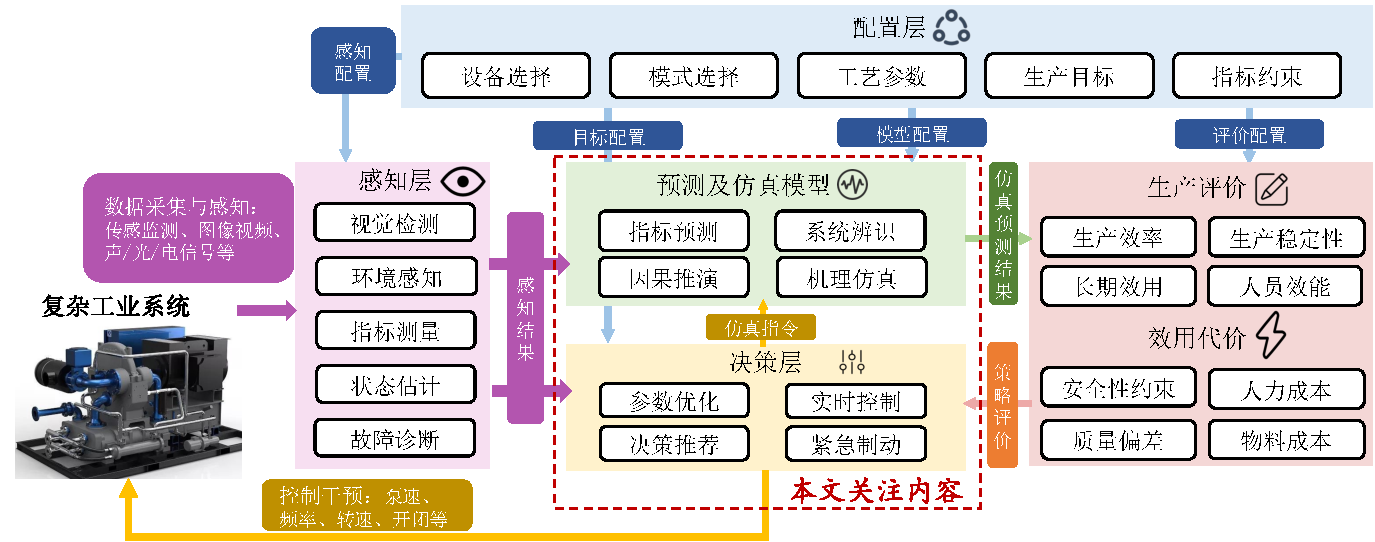
\includegraphics[width=\linewidth]{figures/chapter1/industrial_ai.pdf}
    \caption{
        人工智能技术在复杂工业设备感知、建模、评价、决策领域的应用及技术之间的相关关系}
    \label{fig:industrial_ai}
\end{figure}

在上述体系架构中,感知层作为人工智能领域近十年来的热门研究方向,相较于其他板块发展较为成熟,如状态分类、参量回归预测、目标检测、语义分割等技术,只要训练数据充足,很多场景下可以作为整体人工智能方案中可依赖的模块。
生产评价模块的构建往往依赖于人的经验以及外部限制,比如误差代价、安全约束、运行成本等,需要根据生产目标、系统特性以及外部环境进行针对性设计。
% 从机器智能以及数据驱动可以一定程度上地帮助决策人员发现一些潜在的优化目标以及更长期的效用评价,但能够发挥的作用相对有限。
% 预测与仿真以及智能决策优化作为实现复杂工业系统控制优化的基础,是实现感知、决策、评价一体化闭环智能的关键环节。
% 相较于其他模块而言,现有的预测建模以及决策优化方法在解决复杂系统问题时存在一定局限,严重制约了的工业通用人工智能技术的发展。
% 相较于其他板块而言,现有的预测建模以及决策优化方法在模型适用性、随机性及非线性表示、长时延关系建模等方面存在一定局限,难以适用于特性迥异的复杂工业系统,严重制约了的工业人工智能技术的发展。
相较于其他模块而言,\textbf{现有的预测建模以及决策优化方法在理论体系以及技术方案方面尚不完善,制约了工业人工智能技术的发展。}

% 如何建模复杂系统的运行过程并认知系统的内在机理,是实现系统分析优化的基础。
想要实现复杂工业动态系统建模,并实现系统的决策优化,其本质在于对系统中目标变量的演化机理以及受其他协变量的影响因果关系进行建模,并基于此实现可控变量的逆向优化。
在工业环境下,复杂系统的运行过程存在非线性、高扰动、强耦合等复杂特性,从物理、化学、动力学角度建模系统动态过程的传统分析方法不再适用。
伴随着工业监测技术的不断完善以及生产自动化、信息化水平的不断提升,各种大型设备上安装了用于实时监测生产数据的传感器,
系统运行数据的获取成本逐渐降低,
这使得数据驱动方法成为建模复杂工业系统过程的主流方案,有效突破了理论建模方法存在的局限性。

最早追溯到1950年,为了进行控制系统设计,Zadeh等\cite{zadeh1956identification}首次提出了系统识别的概念用来建模动态系统。
其核心目标是寻找一个与系统“相符”的模型,使得模型预测的输出尽量接近给定系统的真实输出。
以数据为核心驱动力的传统系统识别方法已经逐渐发展为非常完善且成熟的研究领域
\cite{le2013system,gevers2006personal,ljung2008perspectives,ljung2011four,Ljung2020}。
近年来,伴随着人工智能以及机器学习技术领域取得重大突破,传统控制系统建模与优化技术也迎来了新的发展浪潮。
动态系统建模作为一项被前人深入研究数十载的“经典问题”,逐渐朝着观测更高维、动态更复杂的方向演化。

在《关于发布未来工业互联网基础理论与关键技术重大研究计划2021年度项目指南的通告》中指出,“实现动态扰动下系统分布式资源调控、\textbf{数据驱动的系统建模、质量预测与控制以及全流程重构的多目标优化},结合航空航天$\cdots\cdots$。”足以说明数据驱动系统建模技术在现代工业智能化发展中占据着举足轻重的地位。

人工智能界当代最著名巨擘之一、Meta AI实验室主任Yann LeCun,长期致力于让机器对世界的运转理念有基础了解。在其设计的通用人工智能(Artificial General Intelligence,AGI)架构体系中,设计了配置器、短期记忆模块、感知器、决策器、世界模型、评价模型,其中世界模型放在了与感知器和决策器同等重要的位置上。理想的世界模型能够像拥有“常识”的人类一样,预见给定行为将产生的后果,并辅助智能体决策。
本文探究的动态系统建模问题可以认为是世界模型在低维控制、低维观测限定下的特例。
图\ref{fig:industrial_ai}中定义的单个复杂控制系统的感知、建模、决策闭环可以视为一个封闭的“小世界”,本质上与LeCun提出的通用人工智能研究范式极其相似。

从机器学习的视角来看,系统建模本质上是一种有监督学习问题\cite{jordan1992forward}。
对于动态模型,假定其系统状态表示为$s_t$,系统输入为$a_t$,给定批量的状态转移数据,我们可以学习前向模型$\left(s_t, a_t\right) \rightarrow s_{t+1}$,即给定当前状态和动作,预测下一时刻状态。
% 对于所有的基于模型的强化学习,均需要关注于前向模型的构建。
由于现实生活中大部分的客观物理系统具有连续动作空间以及高维观测空间,依赖于表格存储形式的前向模型表示方法难以适用。
函数近似也因此成为当前复杂动态系统建模问题的主流方法,
如线性回归\cite{silver2008sample}、动态贝叶斯网络、随机森林、最近邻搜索、神经网络\cite{werbos1989neural}。
近十年来,深度神经网络以其极强的特征提取与非线性表示能力成为解决高维、大数据、多模态机器学习问题的常用解决方案。
基于深度网络模型的复杂系统建模方法逐渐受到大家的关注,该方法利用神经网路的前向传播过程模拟系统的动态方程\cite{temeng1995model, tan1996nonlinear},再用系统离线数据训练网络参数。
相比于其他方法,神经网络能够很好地扩展至高维输入输出空间以及非线性系统,
且其连续可微的特性能够有效适配基于梯度优化的控制决策算法。
% 特别地,循环神经网络(Recurrent neural network, RNN)因为存在隐状态,可以更好地处理长期预测问题并对系统进行建模\cite{delgado1995dynamic, zamarreno1998state}。
因此,本论文的讨论内容也限定在基于深度学习的系统建模方法中,具体研究面向不同类型动态系统建模问题的网络设计以及学习方法。

% \subsection{微分方程网络在复杂系统建模中的应用}

依托于数字计算机技术的应用普及,以及近年来机器学习、强化学习\cite{sutton2018reinforcement}、深度学习\cite{lecun2015deep}\cite{duan2016}、时间序列分析等技术\cite{shumway2000time}的快速发展,
离散时间(Discrete-time, DT)域下的动态系统建模研究涌现出了诸多成果,领域发展相对较为成熟,其原因与数字计算机将信息离散化的思想密不可分。
相较于离散时间系统,连续时间(Continuous-time, CT)系统作为最早的系统辨识研究范式,近年来其相关理论体系研究较为滞后。在当今数据驱动与深度学习盛行的时代背景下,连续时间模型尚未与主流技术形成深度融合。但是对比离散时间系统建模方法,从连续时间域角度进行系统建模的思想在\textbf{与物理属性的兼容性、引入先验知识的难易度、处理非均匀采样数据、可变采样间隔、计算效率与精度的可调节性、刚性系统建模}等方面具有天然的优势,而上述特性或问题在复杂工业系统中尤为常见。
因此,如何让深度学习等先进的人工智能技术充分赋能传统的连续时间系统辨识及控制决策理论,是推进传统控制领域发展,加速人工智能技术实现产业应用的有效路径。
% 因此,最早的系统辨识方法研究也大多是围绕连续时间系统展开的。

% 神经网络近似能力的通用性可以作为建模非线性系统的一种手段\cite{funahashi1993approximation},进而拟合函数$f$。

% \subsection{基于编解码结构的系统预测}
% 当系统具有较大时延,即高时滞特性下,模型需要考虑历史数据对未来系统变化的影响。Felipe 等\cite{demeester2020system}利用带有Attention组件的Encoder-Decoder模型对一种名为膏体浓密机系统进行建模识别,Yuan等\cite{Yuan2020}采用一种更复杂的名为双注意力循环神经网络(Dual Attention Recurrent Neural Network, DARNN)的RNN网络对工业系统进行建模,两种方法都考虑了系统变量之间的长期依赖性,利用循环神经网络加Attention机制的强大编码能力,对历史数据、不同维度数据进行信息编码,来辅助输出量的预测,并且利用预测误差对编码器部分进行训练调整。然而两种方法都是针对离散时间系统设计的,不适用于连续时间系统建模问题。
% \section{深度微分方程网络}
% \subsection{深度微分方程网络总描述}
% \subsection{微分方程网络概述}
荣获神经信息处理会议2018(Neural Information Processing,NIPS 2018)最佳论文奖的《Neural Ordinary Differential Equations》\cite{chen2018neural}提出了一种常微分方程神经网络,其采用神经网络参数化微分方程的向量域\cite{kidger2021},
成功搭建了连续时间微分方程与深度学习技术之间的桥梁。
在其基础上,神经受控微分方程\cite{kidger2020neural}、神经随机微分方程\cite{li2020scalable}、神经偏微分方程
\cite{li2020fourier}等其他神经微分方程(Neural Differential Equations, NDEs)被相继提出。
许多流行的神经网络架构,如残差网络、循环神经网络均可以视为神经微分方程的离散化形式。
神经微分方程网络兼具现代机器学习以及传统数学建模方法的优势,包括复杂函数的强拟合能力、便于在模型空间中引入强先验假设、处理非均匀采样数据、训练显存占用低等优点。
该范式一经提出就受到了国内外学者的广泛关注,并应用于时间序列分析、时间点过程分析、动态系统建模、可逆生成模型等领域。


% 微分方程网络因其在显存空间占用、系统先验引入、非均匀采样序列处理等方面具备的显著优势,
% 一经提出就受到了国内外学者的广泛关注,并应用于时间序列分析、时间点过程分析、动态系统建模、可逆生成模型等领域。
% 许多流行的神经网络架构,如残差网络、循环神经网络均可以视为神经微分方程的离散化形式。

% 在处理时间序列问题方面,相比于RNN等离散时间步下的循环神经网络。ODE-Net天然地适用于建模非均匀采样的时间序列。

% 因此神经微分方,
% % 因此开辟了解决连续时间系统建模问题的新途径。
% % 神经微分方程网络兼具现代机器学习以及传统数学建模方法的优势,包括复杂函数的强拟合能力、便于在模型空间中引入强先验假设、处理非均匀采样数据、训练显存占用小等优点。

对于大部分工业系统,
% 其底层运行机理遵循化学、动力学、热力学等能够用微分方程描述的基本定律,
其底层运行机理所遵循的化学、动力学、热力学定律均可用连续时间微分方程描述,这与微分方程网络的基本特性极其契合。
% 因此利用连续时间网络模型对物理系统进行建模可以更好地匹配客观世界物理规律,且增加模型的可解释性。,
因此,NDE成功开辟了解决连续时间域下复杂系统建模问题的新途径。
\textbf{然而在工业领域中,大部分的动态系统机理复杂、特性迥异,基于单一前馈神经网络的神经微分方程无法适用于所有建模任务。同时,对于如何利用训练得到的神经微分方程模型指导目标系统的优化控制,存在一定的研究空白。}
为了解决上述建模难的问题,需要结合被建模系统的固有特性、训练数据的统计规律、辨识模型的预测需求,设计合理的参数化模型结构,并选用合理的优化目标与训练方法以获得最佳的建模效果。
因此,本文以膏体充填过程中的深锥浓密机、膏体制备系统为对象,面向长时延非线性、周期多阶段性、随机性三种复杂特性,提出了三种基于常微分方程网络的系统辨识模型,
并在辨识模型的基础上,提出了连续时间域下的复杂工业系统在线优化控制方法。
本文给出的算法与技术成功应用于工业实践,有效推动了深度学习技术在真实工业系统建模与决策场景下的落地。
% 该项研究能够有效拓宽连续时间域下深度学习技术及神经微分方程网络的应用边界,
同时,也为数据驱动的工业系统建模与优化领域开创了新的研究思路。
\section{本文研究的关键问题}
\label{sec:challenge}
% 现有的基于机器学习的系统预测方法多从离散时间域角度描述系统动态过程,并利用数据驱动的方式对离散时间系统参数进行拟合训练。
% 但在复杂工业系统中,上述陈列的系统特性以及问题需求是时常存在的。
% 比如由于不同传感器工作频率不一致会导致数据存在非均匀采样情况,使用离散时间域模型之前需要对数据进行大量的前处理,这会对数据的原始特性造成损坏。

% 连续时间域模型对于复杂动态系统具有天然契合性,深度学习方法在参数化建模与复杂系统表示方面具有较大优势。
% 因此,本论文从二者结合的角度,对基于深度微分方程网络的复杂动态系统预测技术开展研究。
% 利用参数化的深度神经网络模型拟合复杂系统的微分方程,并基于拟合模型实现系统的预测、控制与优化。
神经微分方程网络兼具了深度学习模型的强拟合能力与微分方程的连续时间演化特性,
% 使用连续时间域的深度神经网络模型拟合复杂动态系统,会面临以下研究难点与挑战:
但是使用该模型拟合复杂动态系统时,由于系统存在各类复杂特性,常规网络结构及建模方法会面临以下研究难点与挑战:
\subsection{具有长时延、强非线性的复杂连续时间系统建模问题}
% 随着大数据采集与处理技术的不断进步,很多企业会在复杂工业设备上安装大量传感器以监测工业系统的实时运行过程。
% 为了解决复杂系统的控制决策难题,模型预测控制方法利用传感器监测工业系统的实时运行数据并训练时序预测模型,然后采用基于预测模型的系统优化及控制策略对可控变量进行优化~\cite{Yuan2020,Member2019,wu2020optimization}。
现有的辨识与预测方法在解决复杂工业系统建模问题时难以解决两方面问题,首先大多数工业系统都有极其复杂的高阶动力学方程,而非仿射系统或线性系统,经典的系统假设及参数估计方法难以适用。
另外,对于具有长时延的复杂系统,当前系统输出的变化可能受很长一段时间内系统外部输入的影响,直接建模输入输出之间的微分方程难以从数据中捕捉系统的长时延特性。
% 其次,现有的大多数基于深度学习的系统建模及预测方法~\cite{Member2019,Essien2020,9161367,9522017,neu2021systematic}都是基于离散时间域的,忽略了系统的连续时间特性。从模型结构与系统本体的一致性角度来看,忽视系统本身具备的物理先验特性会增大模型的假设空间进而导致增加拟合难度,在数据集有限的情况的下,限制了模型精度。
% 最后,基于数据驱动的自回归系统辨识模型受制于预测过程累积误差的存在,难以同时处理系统短期预测和长期预测。
最后,原始的常微分方程网络对导函数不断进行积分,其模型本质类似于在离散时间序列预测问题中学习序列的差分,在短期预测时模型精度较好。但在长序列开环预测时,对导数持续积分会造成极大的累积误差。

因此,本文围绕连续时间域下的深度系统辨识模型展开研究,
以解决长时延、非线性复杂动态系统的长短期开环预测问题。



\subsection{具有随机性的连续时间系统建模问题}
现存的连续时间系统辨识及动态系统建模方法,如Time-Aware RNN\cite{Demeester2019}、SNODE\cite{Quaglino2019} 仅在确定状态空间构建系统的动态模型。
由于确定性模型没有引入任何随机成分,不便于实现蒙特卡洛随机采样,这使得某些基于随机采样预测的控制规划方法,如交叉熵(Cross entropy Maximum,CEM)、蒙特卡洛树搜索(Monte Carlo Tree Search,MCTS)难以与此类系统建模方法配合使用。
另外,确定性模型无法适用于建模带有随机性的系统。当被辨识系统的状态转移过程本身具备较强的随机性时,可以近似认为可状态之间的转移过程服从包含隐变量的随机分布,理想的辩识模型应该能够直接对隐变量的转移分布进行建模,
% 如离散时间域下的循环状态空间模型\cite{Hafner2019}(Recurrent State Space Model, RSSM)。
最后,确定性模型无法对系统当前状态的转移分布进行表示。
在现实世界中,尽管很多系统的转移过程本身是确定的,但由于其观测空间的不完备性,从可观测的输入输出数据中无法准确推理系统的完整状态,从结果来看这种不完全观测性也是系统存在随机性的主要原因。

现有连续时间域的系统辨识方法仅能在隐空间中通过最小化误差期望的方式学习状态转移的均值,而无法实现分布表示与状态采样,不仅制约了模型的拟合精度,也难以应用在随机优化问题中。
% 在建模随机随机系统方面,深度时序生成模型~\cite{Fraccaro2016,Chung2015,Karl2017}将标准的变分自编码机(Variational Auto-encoders,VAEs)~\cite{kingma2013auto}扩展到序列情况下,
% 通过在隐空间引入随机隐变量学习序列的随机性,然而这些方法均是离散时间域模型。
因此本文着重研究存在随机性的复杂连续时间系统建模方法,使辨识模型能够对系统动态的随机转移进行拟合,并在给定观测数据下评估系统的随机性与不确定性。

\subsection{具有周期多阶段性的连续时间跳变系统建模问题}
跳变系统是一种在多个子阶段之间随机切换的非线性系统,每阶段下的系统动态方程彼此不同,在每个阶段内的滞留时间会同时受到内部和外部因素的影响~\cite{WANG2022111790}。
为了从给定数据中学习连续时间跳变系统,以往的研究一般限定了系统的先验结构,采用EM算法 (Expectation-Maximization Algorithm)\cite{balenzuela2022parameter}、序列蒙特卡罗(SMC)\cite{6859280}和变分推理\cite{opper2007variational}等方法估计系统参数。
上述方法通常依赖于对系统结构和阶段滞留时间分布的先验认识,
% 这对于部分复杂“黑盒”跳变系统来说是极其困难的。
而对于部分复杂的“黑盒”跳变系统,这些先验知识是难以获得的。
% 这需要大量的领域知识支撑。
% 但是,系统结构和参数往往是未知的,阶段转换时间也并非服从理想的指数分布。
% 但是对于部分复杂的“黑盒”跳变系统,系统结构和参数均是未知的,阶段转换时间也并非服从理想的指数分布。
% 跳变系统建模的另一个困难是数据集中可能同时涵盖多个具有不同动态特性的多个子过程,不同子阶段之间的转换规则很难识别。
以往的一些研究采用基于深度学习的自适应性模型识别此类具有多个子过程的复杂时变“黑盒”系统。
% 深度状态空间模型~\cite{Deep_state_space_model}利用参数动态变化的线性状态空间模型建模系统输出,并引入循环神经网络(Recurrent Neural Network, RNN)建模参数的演化过程。
如Embed to Control(E2C)~\cite{Watter2015}和卡尔曼变分自编码器(KVAE)~\cite{Fraccaro2017}采用多个时不变的线性状态空间模型建模系统在隐空间中的不同动态,并推断出随时间变化的权重$\alpha(t)$以分配每个线性状态空间模型的权重。
此类建模时变动态系统的混合模型假定目标系统由多个“黑盒”子系统按权重混合而成。
而在某些情况下,对于一些自切换的跳变系统,系统在某一时刻的所处阶段是唯一的且阶段转移边界是明确的。
目前尚无研究将系统阶段转移的先验知识引入到辨识模型的设计中,以预测跳变系统中的阶段自切换。  
另外,对于带有多输出项的工业系统,其输出空间同时存在稳定和非稳定过程\cite{nason2006stationary}。
目前,现有的未经过特定设计的预测模型难以解决此类带有混合时序特性的多输出系统学习任务。

因此,本文将着重研究具有多输出量的连续时间跳变系统建模方法,针对多阶段之间周期性转换以及稳定、非稳定输出共存的跳变系统,提出基于常微分方程网络的系统辨识模型,依赖已知的系统先验特性提高模型的辨识精度。

\subsection{复杂工业系统的无模型控制优化问题}
大部分复杂工业生产过程往往伴随着较强的非线性、随机性、高时滞性,因此难以建立准确的数学模型近似其运转机理, 导致传统的控制优化方法无法适用于此类复杂工业设备。
% 为了解决复杂工业设备难以建立准确的数学模型,导致传统的控制优化方法无法适用于此类复杂工业设备。
目前业界对基于强化学习理论的最优控制技术\cite{Sutton2018,F.L.LewisD.Vrabie2012}寄予厚望,希望能够以免模型、数据驱动的方式实现复杂工业系统的自适应优化控制。
% Wei等\cite{Wei2014}将煤炭气化过程的最优追踪控制转化为双人零和最优控制问题,并采用包含控制网络、模型网络、评价网络的迭代自适应动态规划方法求解最优控制律,同时给出了收敛稳定性的分析。
% Jiang等\cite{Jiang2018}利用穿插学习策略迭代(Interleaved Learning
% Policy Iteration, ILPL)并同样采用三网结构实现了对浮选过程操作指标优化的控制,获得了比传统值函数迭代(Value iteration, VI)、策略迭代(Policy iteration, PI)算法更佳的控制效果。
然而,考虑到工业过程试错成本高,大部分强化学习算法随机设定策略模型的参数,在模型训练初始阶段,难以保证生产控制过程的安全。
另外,在工业场景下进行设备在线控制对算法的实时性要求较高。
为了保证控制模型的控制效果,控制系统需要采用实时生成的数据对网络进行训练,使得训练过程产生较大的时间开销,难以保证模型更新与推理的实时性。
同时,在线采样数据时常是间隔非均匀的,大部分离散时间域下的强化学习算法难以适用。
最后,受限于无模型强化学习存在采样数据需求量大与不同场景下泛化能力差等缺陷,无模型强化学习算法在真实的工业实践中难以部署应用。

因此本文研究连续时间域下基于模型的复杂工业系统优化控制策略,充分利用系统运行时的非均匀采样离线数据构建预测模型,并在辨识模型的基础上,构建具有在线自学习能力的控制决策模型。
% 能够适应物料性质改变、设备老化等被控系统不断变化的情况。

\section{本文的研究内容}
% 针对上述问题与挑战, 本文以具有连绔时间动态特性的复杂系统作为研究对 象,针对系统存在的非线性、随机性、多阶段混合、高时延、不同输出量统计特 征不一致等特性, 将连绔时间域模型的灵活性与深度神经网络的强大表示能力相
% 针对第\ref{sec:challenge}节提出的系统存在的高时延、非线性、随机随机性、周期多阶段性、不同输出量统计特征不一致等复杂特性特性,
针对第\ref{sec:challenge}节列出的复杂工业系统难以建模预测及优化控制的问题。
% 本文以具有连时间动态特性的复杂系统作为研究对 象,针对系统存在的非线性、随机性、多阶段混合、高时延、不同输出量统计特 征不一致等特性, 将连绔时间域模型的
本文以具有连续时间动态特性的复杂系统为研究对象,
针对系统存在的非线性、随机性、多阶段混合、高时延、不同输出量统计特征不一致等问题,
依托于连续时间域模型的灵活性与深度神经网络的强大表示能力,研究基于连续时间深度微分方程网络的系统建模及辨识方法。
并在辨识模型的基础上,研究基于有模型强化学习理论的在线优化控制方法,并应用于工业实践。
% 针对复杂系统存在的非线性、随机性、多阶段混合、高时延、不同输出量统计特征不一致等特性,本文开展了如下几方面的研究:
图\ref{fig:study_goal}展示了本文研究内容、研究目标以及不同应用场景的对应关系。
\begin{figure}[h]
    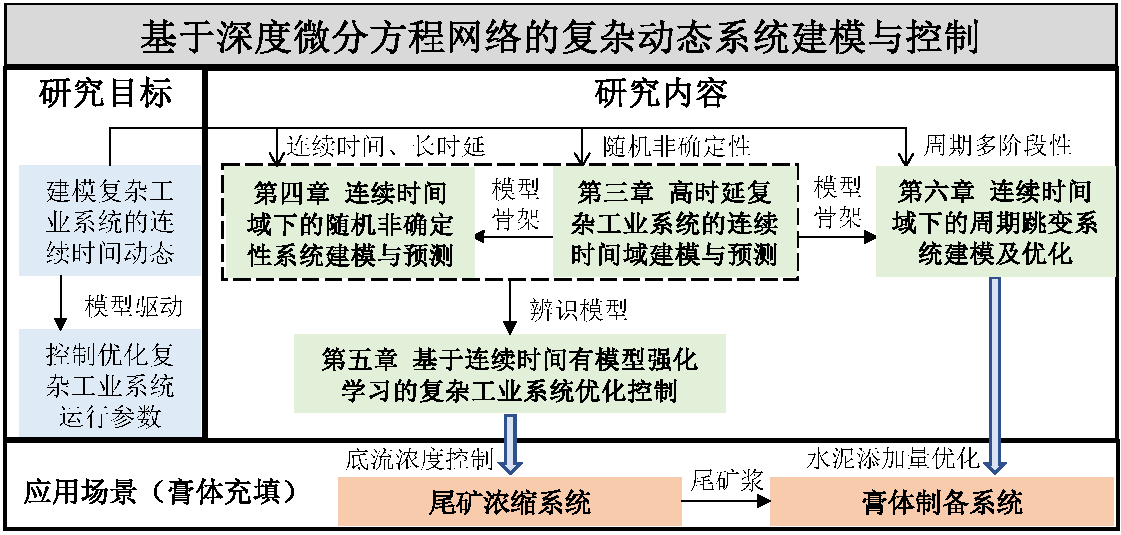
\includegraphics[width=\linewidth]{figures/chapter1/study_goal.pdf}
    \caption{本文研究内容、研究目标、应用场景的对应关系}
    \label{fig:study_goal}
\end{figure}
接下来,将给出每一项研究内容的研究思路和简要介绍。

\subsection{\TitlechapterI}
第一项研究内容“\TitlechapterI”,重点讨论了连续时间视角下,非线性、高时延系统的系统建模问题。
由于大部分工业系统运行过程遵循连续时间特性,使用连续时间辨识模型与系统的机理先验更佳契合。
另外,大部分复杂工业系统反馈延迟长,现有辨识方法难以拟合长距离的依赖关系,直接利用状态空间模型对系统状态和输入记忆进行压缩是极其困难的。
% 会学习过程引入了极强的复杂性与非线性。
想要将深度学习模型的长距离依赖提取能力引入到连续时间辨识模型中,
% 另外基于数据驱动的自回归系统辨识模型受制于预测过程累积误差的存在,难以解决系统的长期预测问题。
因此需要从探索\textbf{参数化微分方程网络对于客观世界连续时间过程的可拟合性}这一科学问题出发,研究深度学习网络与连续时间过程相结合的系统建模方法。

本文的第一个研究内容为了克服动态系统存在的非线性、非仿射的高复杂性。研究了基于深度学习的复杂工业系统建模方法,同时为了契合生产设备运转的连续时间特性,提出以ODE-Net作为模型骨架结构辨识模型,从连续时间域角度拟合目标系统的受控动态过程。
针对系统输入输出之间长时延依赖关系难以建模的问题,研究了基于序列自编码器模型的输入输出长距离信息连接通道构建方法。
针对深度自回归序列模型受制于累积预测误差存在,难以有效进行长期预测的问题,基于时间序列稳定性理论,分析了普通常微分方程网络在长期预测中的非稳定特性,并提出两种分别适用于短期预测和长期预测任务的导数模块定义方法。同时,针对ODE-Net网络训练需要连续控制输入信号的问题,研究了面向训练过程的离散输入点并行插值方法。最后,提出了一套由序列编码器、状态解码器和导数模块组成的深度连续时间(Continuous Time, CT)系统辨识网络,该模型能够以端到端的方式学习工业系统输出的自回归变化过程和输入对输出的非线性影响。
通过消融实验探究了编码器输入序列长度设定、微分方程求解器选择对于预测精度的影响。最后,通过某真实铜矿场中膏体浓密机的运行数据验证了本文提出方法对于解决长时延、非线性工业系统长短期预测问题的有效性。


% 针对复杂工业系统本质上为连续时间演化过程,且存在非线性、长时延等特性,本文提出以ODE-net作为模型骨架结构,从连续时间域角度拟合复杂工业系统的动态过程。




\subsection{\TitlechapterII}
% 3) 基于常微分方程-循环状态空间模型的随机系统建模 \\

第二项研究内容“\TitlechapterII”重点讨论了连续时间视角下,对于随机性系统以及非均匀采样场景下系统建模时会遇到的诸多问题。
第二项研究内容“\TitlechapterII”重点讨论了非均匀采样场景下,对于随机性系统进行拟合建模时会遇到的诸多问题。
现实世界中的复杂系统往往具备典型的随机性(uncertainty),确定性系统辨识模型只能以最小化期望误差的方式拟合系统随机演化函数在某分布下的期望,不仅不便于实现系统的随机采样预测,且无法对可观测数据呈现出的随机性给出表示与度量。因此,想要在辨识模型中引入对于系统随机转移的建模能力,并给出概率域下的状态转移分布的显示描述,需要从“\textbf{部分可观测马尔可夫决策系统的随机性表示}”这一科学问题出发,研究贝叶斯视角下系统隐空间状态的时序生成过程及逆向推理方法。

具体地,该研究内容针对随机性系统难以建模的问题,
研究如何向确定性微分方程系统演化中添加随机转移路径,
进而提出深度常微分方程与马尔可夫模型相结合的随机性系统建模方法,并结合时序变分推断理论给出训练模型所需要优化的证据下界。
同时,针对训练阶段下原始时序变分推理算法无法实现沿时间反向传播(Backpropagation through time, bptt)难以保证多步预测精度的问题,
研究了基于采样状态重用的高效隐空间超调技术,在不增加训练时间开销的情况下显著提升模型的开环预测精度。
最后,针对训练阶段批数据中不同常微分方程积分区间不一致导致难以并行化训练的问题,研究了基于重参数变换的批常微分方程并行求解技术,成功实现了不同积分区间下的高效并行训练。
最后,通过三个输入输出系统数据集验证了本文提出方法对于解决随机性系统多步开环预测问题的有效性。


\subsection{\TitlechapterIII}
第三项研究内容“\TitlechapterIII”重点讨论了连续时间域下,基于数据驱动的复杂工业系统优化控制方法。
由于大部分复杂工业系统的运行过程具有不完全观测、非线性、多变量、高时滞等特点,
想要建立准确的数学模型描述其运转机理是极其困难的,因此基于模型的传统最优控制理论及方法难以适用。另一方面,系统运行过程产生的历史数据为实现数据驱动的优化控制提供了可行性。
% 想要充分利用离线数据构建近似的系统模型并衍生形成可靠的控制策略,
% 需要从“\textbf{数据驱动建模对于免模型强化学习的可改善性}”这一科学问题出发,研究基于辨识模型指导的复杂工业系统强化学习控制方法。
% 想要利用系统离线运行数据构建可靠的控制策略,
% 需要以动态系统辨识为前提,进一步研究基于辨识模型的复杂工业系统控制策略构建方法。

该研究内容针对非线性、高时滞复杂工业系统控制优化难的问题,研究了连续时间域下的自适应动态规划控制方法,定义了被控系统的状态空间、动作空间、效用函数、状态转移函数,同时提出了离线系统建模与在线强化学习相结合的控制器构建及生产环境在线更新策略,
% 通过利用离线采集数据以及在线监测数据有效解决了复杂工业系统控制优化难的问题。
另外,针对在线环境下策略网络增量训练开销大、在线学习与控制难以满足实时性的问题,研究了基于自适应评价值迭代的控制动作求解算法,
结合评价网络与模型网络的长期效用评估能力,采用梯度优化算法直接求解控制指令,避免控制网络在线学习的计算开销。
与此同时,针对传统自适应动态规划算法中评价模块参数收敛慢、难以准确给出策略优化方向的问题,本文研究了基于短期经验回放的评价网络训练技术,有效提高了模型对于局部评价值梯度变化的敏感性及预测准确性。
最后,本文选用尾矿浓密机仿真模型验证了本文提出的自适应控制算法在控制精度、时间消耗方面的优势。
同时将该控制算法应用于某真实矿山的深锥浓密机底流浓度控制场景中,相比于原始的规则控制算法,大幅度提高了出料浓度的追踪控制精度及稳定性。

\subsection{\TitlechapterIV}


% 2) 基于有限状态机-常微分方程网络的周期性多阶段复杂系统建模 \\
第四项研究内容“\TitlechapterIV”重点讨论了连续时间视角下周期跳变系统建模问题。
% 某些工业场景中,系统运行呈现多阶段特性,
某些工业系统的运行过程呈现周期多阶段特性,
系统在不同阶段下的动态方程彼此迥异,且各阶段的持续时间、状态跳变的触发条件会同时受到内部、外部多种混杂因素共同影响。
% ,其影响机理复杂,可能超出领域知识的可解释范畴。
想要结合参数化深度模型对具有跳变特性的多阶段系统以端对端的方式进行数据驱动建模,需要从探索\textbf{跳变系统阶段滞留时间及转移机制的可学习性}这一科学问题出发,
研究符合跳变系统先验且具有阶段自识别、自转移能力的多阶段深度辨识方法。

具体地,该研究内容针对周期多阶段系统在不同阶段下动态特性差异大,难以统一建模的问题,
研究了传递式多ODE-Net集成结构,以独立建模系统在不同阶段下的动态特性,并在开环预测时,支持阶段转换处隐空间状态的衔接。
针对阶段持续时间难以预测、转换条件和位置难以识别的问题,
本文提出了跳变系统辨识问题中的自跳跃(Autonomous jump)概念,
并在多ODE-Net集成架构的基础上,研究了基于阶段持续时间预测网络的阶段自转移方法。
除此之外,针对工业系统多输出项可能同时存在稳定特性和非稳定特性的情况,研究了面向不同类别输出项的解耦建模方法,并提出了稳定ODE与非稳定ODE相结合的分层常微分方程网络单元。最后,利用膏体制备过程的水泥添加系统运行数据验证了本文提出方法在解决多输出、周期跳变系统建模问题的有效性。


\section{论文的章节安排}

本文针对连续时间域下的复杂动态系统建模及控制中的关键技术开展研究,全文共分为七章,各种内容安排如下:
% ,各章主要研究内容及之间的关系如图所示:
% \begin{figure}
%     \centering
%     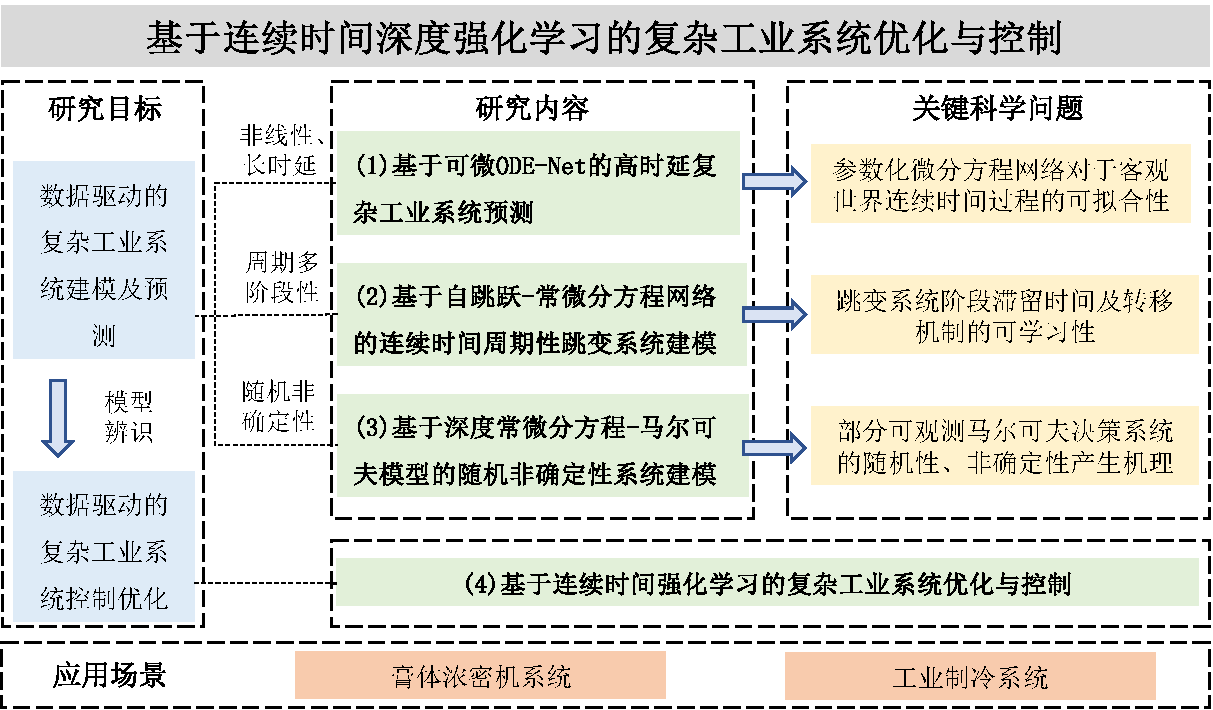
\includegraphics[width=0.95\linewidth]{figures/chapter1/structure.pdf}
%     \caption{论文组织结构}
%     \label{fig:structure}
% \end{figure}

第一章介绍本文工作的研究背景及意义,提出了基于数据驱动的复杂系统建模方法所面临的难点与挑战,并总结了本文的主要研究内容与创新点。
第二章介绍了国内外关于数据驱动的动态系统建模的研究现状。
第三章到第六章是本文的主体部分,详细介绍了本文的所有研究内容。

% 第二章对于复杂系统的预测方法及深度微分方程网络的原理及技术进行介绍。

第三章研究了基于可微ODE-Net的高时延工业多输入输出系统预测,
首先介绍了复杂输入输出系统预测问题的形式化表述,并给出基于状态空间模型的表示方法。
进一步地,介绍了本文提出的基于ODE-Net的连续时间输入输出系统预测模型,并分别介绍其序列编码器、导数模块以及状态解码器三大组成模块,同时给出了基于伴随状态的模型训练方法。
另外,该章针对短期预测和长期预测两种预测场景,给出了两种导数模块定义方法。
并提供了用于连续化系统输入序列的并行插值方法。
最后,该章介绍了将上述模型应用于膏体浓密机系统预测问题的实验结果。并从微分方程求解器的选择、序列编码器输入的长度设定等多个角度进行了消融实验。

% 第三章研究了基于有限状态机-常微分方程网络的周期性多阶段复杂系统预测建模技术,分别介绍了周期性多阶段系统的形式化定义,H-ODEnet结构设计,DFA-ODEnets模型结构设计、基于DFA-ODEnets的编码器解码器结构设计。


第四章研究了基于深度常微分方程-马尔可夫模型的随机性系统建模,首先给出了非均匀采样下随机系统的形式化描述及符号变量定义。
技术部分首先介绍了本文提出的常微分方程-循环状态空间模型,包括其时序受控生成过程及隐变量的后验推理过程。
并基于时序变分推断方法给出了用于训练模型的单步证据下界。
进一步地,为了改善模型的多步预测性能,在单步下界的基础上提出了基于隐空间超调的多步变分下界。
最后,提出了非均匀采样间隔下的批量常微分方程并行化求解方法以加速训练。
实验环节采用两个共有数据集和一个私有数据集对常微分方程-循环状态空间模型以及多个基线模型在非均匀采样设定下的随机采样系统建模问题的有效性进行评估,并对多步预测性能
实验环节采用两个共有数据集、一个私有数据集对常微分方程-循环状态空间模型以及多个基线模型进行对比评估,
同时验证了隐空间超调技术对于多步预测的改善效果以及非均匀间隔批常微分方程并行求解算法的有效性。

第五章研究了基于连续时间有模型强化学习的复杂工业系统优化与控制,
首先,该章基于连续时间强化学习理论给出系统优化控制的符号变量定义以及形式化描述。
然后,描述了如何利用神经常微分方程构建模型网络以近似被控系统的动态方程。
进一步地,结合积分强化学习理论给出折扣积分奖赏的定义及表示形式,并介绍如何利用评价网络对策略评价值进行近似。
同时,该章提出了启发式评价网络值迭代控制算法,该算法利用评价网络与模型网络的预测、评价能力,结合随机梯度下降法生成控制指令。
最后,该章提出了短期经验回放技术以提升预测局部评价值梯度的准确度,
% 最后,本文选用一种典型的复杂工业系统——尾矿浓缩机,利用其仿真模型验证了本文提出的自适应控制算法在控制精度、时间消耗方面的优势。
% 同时将该控制算法应用于某真实矿山的深锥浓密机底流浓度控制场景中,相比于原始的规则控制算法,大幅度提高了出料浓度的追踪控制效果及稳定性。
实验环节评估了该章提出的控制算法在浓密机仿真模型及某矿山真实深锥浓密机底流浓度控制问题中的有效性。

第六章研究了基于自跳跃常微分方程网络的连续时间跳变系统建模。
首先给出了连续时间跳变系统的变量符号定义以及系统预测问题的形式化描述。
其次,介绍了本文提出的分层常微分方程网络的定义及结
构,及如何将其用于学习同时带有稳定和非稳定时间序列输出的动态过程。
再次,提出了用于建模连续时间周期跳变系统的自跳跃常微分方程模型,并详细阐述了其状态转移方程、持续时间预测器等关键模块结构的定义。
进一步地,给出了基于该模型的编码器解码器框架及其训练方法。
最后,实验环节介绍了如何将上述框架应用于
% 模拟某实际工业制冷系统,预测给定热负载下的制冷功耗以及出气口温度变化,
建模膏体制备系统中的水泥添加过程,预测给定浓密机出料浓度及流量下的水泥消耗以及膏体浓度变化,
同时基于预测仿真结果,对控制水泥添加系统启停的浓度设定值进行优化。

% todo: 本文总结的部分要加一些
第七章对本文各章的主要研究内容和创新点进行了回顾,并总结了本文工作在基于深度学习的连续时间动态系统辨识领域所作出的学术贡献。
同时,该章围绕机理先验与数据驱动算法结合的混合动态模型构建这一领域,
% todo: 下一句话需要润色
分析了向模型中引入系统先验知识的实现思路,
并分别从机理模型参数建模、残差拟合、基于先验指导的网络设计三个方面,讨论了现有方法的优势与局限,
最后,对该领域未来的未来研究方向做出了展望。


% 第二章
\chapter{文献综述}
    
% 当前,新一轮科技革命和产业变革加速发展,新一代信息技术正在与工业生产 深度融合,自动化、信息化、智能化已经成为全球工业制造发展的重要方向。
% 2020年李克强总理发布的《政府工作报告》中,明确提出“推动制造业升级”、“推进智能制造”的要求。如何工业生产利用智能化技术,将,

% 为了实现工业4.0、工业互联网、数字孪生等伟大技术愿景,其中


% 复杂工业系统的控制与优化是典型的交叉学科,计算机、自动化、控制工程、仪器仪表等。
% 伴随着人工智能与数据科学的发展,数据驱动的复杂系统建模与控制优化技术逐渐应用。
% 现存问题:如何合理地将深度学习与工业过程特性深度融合,同时有效地指导系统优化并实现智能控制,对此部分的研究迫在眉睫。
% 本文面向具有长时延特性、周期多阶段性、非确定性的三类复杂工业系统,提出一套基于ODE-Net的动态系统建模方法,并在构建模型的基础上,提出了基于有模型强化学习理论的控制优化方法,并成功应用于工业实践。实现了xxx目标,为数据驱动的工业系统建模及控制优化提供了新的研究思路。
\section{动态系统辨识及有模型控制的起源与发展}

% 基于数据驱动的复杂工业系统预测建模方法可以分成两大类:离散时间(Discrete Time, DT)系统建模和连续时间系统建模。

从机器学习的视角来看,系统建模本质上是一种有监督学习问题\cite{jordan1992forward}。本节主要从模型参数估计方法以及基于模型的优化控制两方面对动态系统辨识及有模型控制进行简要介绍。

对于动态模型,假定其系统状态表示为$s_t$,系统输入为$a_t$,给定批量的状态转移数据,我们可以学习前向模型$\left(s_t, a_t\right) \rightarrow s_{t+1}$,即给定当前状态和选择的动作,预测下一个状态。对于所有的基于模型的强化学习,均需要关注于前向模型的构建。为了利用有监督学习算法学习上述前向模型,可以采用参数化方法和非参数化方法两种方式,进一步按照模型是否有随机性分类分为确定性模型和非确定性模型两种。

非参数化的系统建模方法直接存储以及利用历史数据进行动态模型的表示与预测。
非参数化方法可以进一步分为精确建模和近似建模。对于精确建模,采用回放池\cite{lin1992memory}方法存储系统的历史轨迹,并将前向预测过程转化为检索问题。
对于非参数的近似建模方法,比较常见的是高斯过程模型\cite{deisenroth2011pilco,deisenroth2011pilco},通过利用历史部分状态-动作点,可以外推预测某一新给定状态-动作点的高斯分布。该方法能够对系统演化的非确定性给出度量。

相比于非参数化方法,参数化方法的参数数量与观测数据集的大小是独立的
。因此,参数化方法也是应用最广泛的模型近似方法。精确参数化方法也称为表格方法,对于每一种可能的转移维护独立的转移概率。如随机马尔可夫决策过程(Markov Decision Process,MDP),基于表格的最大似然模型能够统计每一种转移的概率:
\begin{equation}
    T\left(s^{\prime} \mid s, a\right)=\frac{n\left(s, a, s^{\prime}\right)}{\sum_{s^{\prime}} n\left(s, a, s^{\prime}\right)}
\end{equation}
% where $T$ denotes the approximation of the true dynamics $\mathcal{T}$, and $n\left(s, a, s^{\prime}\right)$ denotes the number of times we observed $s^{\prime}$ after taking action $a$ in state $s$. This approach
$T$代表真实系统$\mathcal{\mathcal { T }}$的近似,
$n\left(s, a, s^{\prime}\right)$ 代表在状态$s$下执行动作 $a$产生状态$s^{\prime}$的频次。表格法作为最简单的系统建模方法,随着状态集$\mathcal{S}$的增大,表格的大小呈指数增加,因此难以扩展到高维问题。

另一种参数化建模的方式是对转移函数进行参数近似,在相似状态之间实现信息的泛化,以充分降低对于存储以及数据量的需求。函数近似也因此成为解决连续空间以及高维动态系统建模问题的主流方法。原则上,可以使用任意参数近似方法学习模型,如线性回归\cite{silver2008sample},动态贝叶斯网络、随机森林、最近邻搜索、神经网络\cite{werbos1989neural}。
近十年来,深度神经网络已经成为解决通用函数近似问题的主流方法,也因此逐渐成为近似动态系统的主流方案。
相比于其他方法,神经网络能够很好地扩展至高维输入输出空间以及非线性系统。
利用神经网路的前向传播过程模型可以模拟系统的动态过程\cite{temeng1995model, tan1996nonlinear}。
特别地,循环神经网络(Recurrent neural network, RNN)因为存在隐状态,可以更好地处理长期预测问题并对系统进行建模\cite{delgado1995dynamic, zamarreno1998state}。
本文的讨论内容也限定在基于深度学习的系统动态建模方法中,研究面向不同类型动态系统的深度网络设计以及学习方法研究。


% TODO

\section{连续时间系统辨识}

% 依托于近年来机器学习、强化学习\cite{sutton2018reinforcement}、深度学习\cite{lecun2015deep}\cite{duan2016}、时间序列分析技术\cite{shumway2000time}的发展与普及,
在过去的几十年间,数字计算机技术发展迅猛。
从离散时间(Discrete-time, DT)角度进行系统建模的研究方向涌现出了诸多成果,领域发展相对较为成熟,其原因与数字计算机将信息离散化的思想密不可分。

相比而言,连续时间(Continuous-time, CT)系统作为最早的系统辨识研究范式,近年来,其相关理论体系研究较为滞后,且在当今大数据、数据驱动的时代背景下,并未与主流技术形成深度融合。但是对比离散时间系统建模方法,从连续时间域角度进行系统建模的思想在某些情况下具有较大优势:
\begin{itemize}
\item	对于物理属性的兼容性:大部分的物理现象都服从连续时间设定,如化学、动力学、热力学等典型场景都可以利用微分方程进行表述,因此利用连续时间模型对物理系统进行建模可以更好地匹配客观世界物理规律,且增加模型的可解释性。
\item	对于先验知识的表示:系统动态不同阶的相关度,如:位移、速度、加速度之间的相关性可以在连续时间系统下非常容易地表示出来,进而有效利用先验知识,降低模型求解的自由度。
\item 潜在的数据滤波:一般的系统辨识过程需要执行特定的预过滤策略以消除数据中的噪音。而连续时间系统建模方法本质上包含了数据预过滤过程。
\item	非均匀的数据采样:当数据采样间隔不均匀时,离散时间方法无法使用,但是连续时间辨识方法能够有效解决非均匀采样问题。
\item	连续时间系统与离散时间系统的相互转换:对于连续时间系统可以通过变更采样率的方法获得任意时间间隔的离散时间系统。而对于离散时间辨识系统,当预测步长与下游应用所需的时间间隔不一致时,模型无法适用。
\item	离散时间模型在高采样率下存在精确性问题:当数据采样率较高时,系统在相邻时刻间的状态变化较小,不适宜的DT模型难以从微小的状态变化中学习系统动态,导致模型的开环预测结果存在精度差、鲁棒性低的问题。连续时间模型本质上学习连续时间域下的微分方程,采样率越高,轨迹越完备,学习效果越好。
\item	钢性系统建模:当系统同时存在快过程和慢过程时,离散采样的间隔选取不当很容易造成快过程或慢过程其中一类统计性质的丢失,对离散时间系统处理造成较大阻碍。而连续时间模型能够从频域角度对不同频率的演化过程进行独立建模。
\end{itemize}
上述七大特性在复杂工业系统中尤为常见。
因此,最早的系统辨识方法研究也大多是围绕连续时间系统展开的。
% \subsection{基于数据驱动的复杂工业系统建模及控制}
系统通常是由表征系统输入输出关系的数学模型描述的,这个模型有其特定的结构和参数。以代数方程表示的系统称为静态系统,
考虑最简单的形式,系统的连续时间模型可以建模为常系数微分方程:
\begin{equation}
\frac{\mathrm{d}^{n} y(t)}{\mathrm{d} t^{n}}+a_{1} \frac{\mathrm{d}^{n-1} y(t)}{\mathrm{d} t^{n-1}}+\cdots+a_{n} y(t)=b_{0} \frac{\mathrm{d}^{m} u(t)}{\mathrm{d} t^{m}}+\cdots+b_{m} u(t)+v(t)
\end{equation}
$\frac{d^{i} x(t)}{d t^{i}}$代表信号$x(t)$对时间的$i$阶导数,该式表示了在任一时刻系统状态对时间的各阶导数与输入量对时间的各阶导数之间存在线性关系。

一般地,对于任意阶数的线性齐次微分方程可以转化为状态空间模型的形式:
% 对上式进行简化,仅考虑状态的最高一阶导数与输入量的零阶导数,并引入非线性成分,得到:
\begin{equation}
    \left\{
    \begin{aligned}
\dot {\boldsymbol h}(t)&=f(\boldsymbol h(t), \boldsymbol{u}(t))\\
\boldsymbol y(t)&= C \boldsymbol h(t)
    \end{aligned}
    \right.
\end{equation}
其中$f$为某一未知函数且具有较强的非线性特性,$\boldsymbol h(t)$代表系统的状态表示,$C$为投影矩阵。
神经网络近似能力的通用性可以作为建模非线性系统的一种手段\cite{funahashi1993approximation},进而拟合函数$f$。

% \subsection{基于编解码结构的系统预测}
% 当系统具有较大时延,即高时滞特性下,模型需要考虑历史数据对未来系统变化的影响。Felipe 等\cite{demeester2020system}利用带有Attention组件的Encoder-Decoder模型对一种名为膏体浓密机系统进行建模识别,Yuan等\cite{Yuan2020}采用一种更复杂的名为双注意力循环神经网络(Dual Attention Recurrent Neural Network, DARNN)的RNN网络对工业系统进行建模,两种方法都考虑了系统变量之间的长期依赖性,利用循环神经网络加Attention机制的强大编码能力,对历史数据、不同维度数据进行信息编码,来辅助输出量的预测,并且利用预测误差对编码器部分进行训练调整。然而两种方法都是针对离散时间系统设计的,不适用于连续时间系统建模问题。
% \section{深度微分方程网络}
% \subsection{深度微分方程网络总描述}
% \subsection{微分方程网络概述}

\section{微分方程网络在复杂系统建模中的应用}
发表自神经信息处理会议2018(Neural Information Processing,NIPS 2018)的一篇开创性文章\cite{chen2018neural}提出了一种常微分方程神经网络,其采用神经网络参数化微分方程的向量域\cite{kidger2021}:
\begin{equation}
y(0)=y_0 \quad \frac{\mathrm{d} y}{\mathrm{~d} t}(t)=f_\theta(t, y(t))
\end{equation}
其中$\theta$代表可学习的神经网络参数,$f_\theta: \mathbb{R} \times \mathbb{R}^{d_1 \times \cdots \times d_k} \rightarrow \mathbb{R}^{d_1 \times \cdots \times d_k}$代表标准的神经网络结构。$y:[0, T] \rightarrow \mathbb{R}^{d_1 \times \cdots \times d_k}$代表微分方程的解。对于大部分应用,$f_\theta$为简单的前馈神经网络。使用神经微分方程的核心是将微分方程求解器作为可学习微分计算图的一部分。

图\ref{fig:neural_ode}给出了一个简单神经常微分方程的计算图。
\begin{figure}[h]
    \centering
    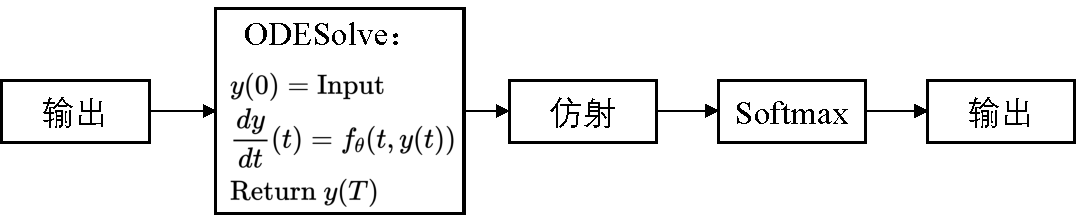
\includegraphics[width=0.9\linewidth]{figures/chapter1/simple_ode.pdf}
    \caption{神经常微分方程的计算图}
    \label{fig:neural_ode}
\end{figure}

ODE-Net的主要应用包括Res-Net的替代、时间序列建模以及可逆正则化流\cite{Grathwohl2019}。本文主要围绕ODE-Net在时间序列建模及系统辨识中的应用展开研究。
因为ODE-Net的连续时间特性,该方法能够将深度网络模型应用于连续时间域下的时间序列建模问题研究中,开辟了时间序列分析、连续时间系统建模研究的新思路。
% 接下来本节将简单介绍几种常见的微分方程网络及其应用。

在处理时间序列问题时,相比于RNN等离散时间步下的循环神经网络。ODE-Net天然地适用于建模非均匀采样的时间序列。如基于ODE-Net衍生的ODE-RNN\cite{10.5555/3454287.3454765}、GRU-ODE-Bayes\cite{brouwer2019gru}、ODE-LSTM\cite{lechner2020learning}。
为了求解ODE-Net的初值,Latent ODE\cite{10.5555/3454287.3454765}将ODE-Net的初始状态视为先验分布为标准高斯分布的因变量,利用编码器-解码器结构实现序列的重构、插值、预测,并使用变分贝叶斯方法对模型进行训练。
文献\cite{Yildiz2019}基于贝叶斯理论,构建了2阶ODE-Net模型用于高维时间序列的建模,同时利用ODE-Net连续正则化流的特性估计待预测时间点隐变量的后验分布并引入分布正则化对隐状态的范围作出限定。

% \subsection{常微分方程网络}
在常微分方程网络求解器效率的优化方面,
% chen等最早提出常微分方程网络化\cite{chen2018neural}开创了深度学习与微分方程结合的先河。
% 为了加速ODE-Net的求解,
Zhuang等\cite{Zhuang2020}提出了自适应检查点联合状态方法以改进原始联合敏感度法求解梯度的精度以及效率。正则化神经常微分方程(regularized neural ODE,RN-ODE)\cite{J2020}基于理论保证的最优传输和稳定性正则化简化ODE系统,能够有效优化ODE-Net的数值积分求解效率。
除此之外,对ODE方程的高阶导数正则化\cite{kelly2020}对求解时间点添加随机扰动\cite{Ghosh2020}等方案也能够起到正则化作用,加速ODE-Net的求解效率。


% \subsection{受控微分方程网络}
由于常微分方程的解仅由初始状态决定,无法基于后续的观测对轨迹进行调节,使得诸如latent-ode、ODE2VAE等模型将序列观测信息全部压缩至初始状态中,有可能造成观测信息的信息损失。
神经受控微分方程(Neural Controlled Differential Equation)\cite{kidger2020neural}将受控信号的微分项融入在ODE网络的求解中。相比于在求解时间区间的间隔点处利用观测数据对隐状态进行更新的方法(如ODE-RNN、ODE-LSTM等),获得了更好的序列信息提取与表示能力。
为了解决神经受控微分方程在长时间序列场景下难以训练的问题,基于对数签名变换(Log signature transform)的Log-signature/NCDE方法\cite{morrill2021neural}通过签名变换对受控信号进行转换,能够增加模型训练速度、减少存储开销、改进模型预测性能。
针对常规的受控微分方程需要对离散序列进行样条插值,无法实现在线预测的情况,Morrill等\cite{morrill2021online}描述了受控微分方程中连续控制信号应满足的性质,并给出了三次埃尔米特直线插值方法,使受控微分方程网络能够类似于RNN一样,实现在线的时间序列数据处理,而不需要预先对完整的序列数据进行插值。
% \subsection{随机微分方程网络}

在常微分方程网络及受控微分方程网络的基础上,随机微分方程网络相比于常微分方程添加了扩散项(Diffusion process)。
对于随机微分方程的训练也可以采用联合敏感度法(Adjoint Sensitibity)进行训练\cite{li2020scalable}。由于随机微分方程网络的前向传播过程依赖于带有随机性的Wiener过程,为了避免存储完整的计算图,需要保证反向求解SDE时对Wiener过程的采样与前向传播保持一致。文献\cite{li2020scalable}利用基于虚拟布朗树(Virtual Brownian Tree)的伪随机数生成策略,仅需常数级存储$\mathcal{O}(1)$即可对的SDE网络前向传播的Wiener过程采样结果进行存储。节约存储空间的代价为对特定时间点下的wiener过程采样时间复杂度为$\mathcal{O}(\log n)$。
将微分方程网络作为Res-Net的替代品处理图像领域问题时,有研究表明将ODE-Net替代为SDE-Net,在ODE-Net中增加随机扩散项,也能够起到随机正则化的作用,提升网络的泛化能力\cite{Oganesyan2020}。
神经跳变随机微分方程(Neural Jump Stochastic Differential Equations,NJSDE)\cite{Jia2019}将扩散项中对时间的微分替换为观测点次数的微分,能够在建模系统隐空间连续时间动态的同时对观测点出现事件本身以及时刻进行建模,该模型有效地应用于地震预测及药物预测。

% \subsection{受控微分方程网络}
% \section{深度微分方程网络的应用}
% \subsection{}
% ODE-Net作为Res-Net的替代,可以应用于图像处理问题中:如图像超分问题\cite{OISR,jia2019focnet}。
在系统辨识领域,
在许多真实的工业场景中,从被识别系统采样得到的序列数据经常是间隔非均匀的。利用微分方程网络模型能够有效建模系统输出或隐空间状态在外部输入影响下的瞬时变化。
Zhong等\cite{zhong2019symplectic}采用ODE-Net对符合哈密尔顿特性的动态系统进行建模学习,巧妙地将物理先验知识融入到学习模型的设计中。并有效地应用于符合哈密尔顿性质的刚体系统建模与控制问题中。
Ayed等\cite{ayed2019learning}采用ODE-Net模型从系统状态的部分可观测信息学习复杂非线性时空过程。该方法有效应用于水流动预测、Navier Stokes方程、海洋温度分析。
% SNODE\cite{Quaglino2019}模型基于勒让德多项式构建ODE-Nets的压缩表示并应用于系统辨识。
SNODE\cite{Quaglino2019}使用谱方法用于快速和准确地训练神经常微分方程模型以辨识低维输入输出系统。
ODE-RNN~\cite{Rubanova2019}在RNN网络相邻状态更新处插入ODE-Net模块,用于建模网络隐状态的连续时间演化。
为了改善辨识模型在长期预测时的稳定性,如本文第三章所述的稳定性模型,现有研究\cite{Demeester2019,Yuan2022}将递归神经网络的稳定性融入到微分方程的导数网络设计中以解决单位根问题,并提出了一种连续时间系统辨识模型——时间感知的RNN模型。

为了建模来自于多智能体系统的非均匀采样数据,LG-ODE模型\cite{Huang2020}将图神经网络、自注意力以及ODE-Net进行结合,利用时序自注意力模型构建微分方程求解的初态,采用图神经网络建模观测点的时序依赖关系和不同观测项之间的空间依赖关系,并以此为基础估计常微分方程中的隐状态导数。模型有效地应用于稀疏序列的插值预测与外推预测。


对于Transformer、AttentionSeq2Seq等基于注意力的序列处理模型,利用ODE-Net的连续时间特性可以构建连续时间注意力模型\cite{chen2021continuous},并将注意力机制应用于非均匀采样的时间序列。
近年来,Transformer模型\cite{Vaswani2017}因在序列数据处理问题上的优异表现受到了学者的广泛关注,基于Transformer的长序列预测模型,如Informer\cite{Zhou2020}、Autoformer\cite{Wu2021}等均获得比传统时序预测算法更优的预测精度。
得益于ODE-Net的连续时间特性,该模型能够与Transformer进行结合,处理非均匀采样数据或长序列预测及建模问题,如构建连续时间注意力\cite{chen2021continuous}、辅助位置编码(position embedding)\cite{Liu2020}。
正因为ODE-Net模型能够利用非均匀采样数据拟合动态系统,因此可用于有模型强化学习\cite{Yildiz2021}领域,构建可微分的系统状态演化估计器,进而辅助策略模块的学习。
对于系统动态已知的连续时间系统,利用ODE-Net可以为策略网络构建连续时间梯度估计器\cite{Ainsworth2020},使控制和仿真任务的学习更高效、更鲁棒。

\subsection{系统长时延特性建模}
近年来,Transformer模型\cite{Vaswani2017}因在序列数据处理问题上的优异表现受到了学者的广泛关注,基于Transformer的长序列预测模型,如Informer\cite{Zhou2020}、Autoformer\cite{Wu2021}等均获得比传统时序预测算法更优的预测精度。
对于Transformer、AttentionSeq2Seq等基于注意力的序列处理模型,利用ODE-Net的连续时间特性可以构建连续时间注意力模型\cite{chen2021continuous},并将注意力机制应用于非均匀采样的时间序列。

得益于ODE-Net的连续时间特性,该模型能够与Transformer进行结合,处理非均匀采样数据或长序列预测及建模问题,如构建连续时间注意力\cite{chen2021continuous}、辅助位置编码(position embedding)\cite{Liu2020}。
\subsection{跳变系统辨识}
连续时间跳变系统包含多个连续时间子系统,且受到隶属有限状态集的内部阶段变量控制\cite{8709809}。
以最简单的连续时间跳变线性系统\cite{fang2002stabilization}为例:
\begin{equation}
    \dot{x}(t)=A(\sigma(t)) x(t)+B(\sigma(t)) u(t)
\end{equation}
% In order to learn the CTJS from available data, previous studies have assumed the prior structures of system and employed methods such as EM algorithm\cite{balenzuela2022parameter}, Sequential Monte Carlo (SMC)\cite{6859280}, and variational inference \cite{opper2007variational} to estimate the ``grey-box'' model parameters.
$A$和$B$为模型参数。
$\sigma(t)$为有限状态随机跳变过程,通常表示为时间自治的、状态有限的马尔科夫过程。

定义状态集$\underline{N}=\{1,2, \ldots, N\}$,对于所有 $i, j \in \underline{N}$,定义状态转移概率矩阵:
\begin{equation}
    \begin{aligned}
    &p_{i i}=0\\
    &q_i=-q_{i i}=\sum_{l \neq i} q_{i l}\\
    &p_{i j}=\frac{q_{i j}}{q_i}, \quad(i \neq j) .
    \end{aligned}
\end{equation}

给定单步转移概率矩阵为$\left(p_{i j}\right)_{N \times N}$,$\left\{r_k ; k=1,2, \ldots\right\}$表示离散时间马尔科夫链,也成为连续时间阶段信号$\{\sigma(t)\}$的嵌入马尔科夫链。相邻跳跃之间的滞留时间用$\tau_k$表示,初始状态表示为$\sigma (0)=i$。过程以概率$p_{ij}$跳跃至状态$j\neq i$,在阶段$j$下的滞留时间服从参数为$q_i$的指数分布。
过程$\{\sigma(t)\}$访问过的状态表示为嵌入马尔科夫链$\left\{r_k ; k=1,2, \ldots\right\}$,相应的滞留时间$\left\{\tau^{\left(r_k\right)}\right\}$是服从独立指数分布的随机变量,分布参数为$q_{i_k}$。
联合过程$\left\{\left(r_k, \tau_k\right): k=0,1, \ldots\right\}$是时间同质的马尔科夫过程,完全确定了跳变系统阶段变量$\{\sigma(t)\}$。

为了从包含多阶段混合数据的离线序列中学习连续时间跳变系统参数$\{A(i),B(i);i \in \underline{N}\}$以及阶段切换参数$\{q_i,p_{ij};i,j \in \underline{N}\}$,Ashley等采用序列蒙特卡洛(Sequential Monte Carlo, SMC)\cite{ashley2014sequential}将辨识问题转换为一般的非线性状态空间估计问题。不过该方法计算量较大。
为了更有效地利用有限的计算资源,随机近似(Stochastic approximation, SA)\cite{svensson2014identification}思想被引入SMC框架中。变分近似方法\cite{opper2007variational}是其中的典型代表。

Balenzuela等提出了一种基于EM算法的马尔科夫跳变系统辨识方法\cite{balenzuela2022parameter}。
为了克服传统方法中E步计算复杂度随阶段数指数增长的问题,该文章提出的EM方法在合并高斯成分的E步内使用近似算法,以减少高斯分量的数量。
原则上,该方法不需要SMC和随机逼近方法中通常需要的渐近参数,就可以得到精确解。

Opper等\cite{opper2007variational}提出采用平均场理论,在给定有噪音的观测数据下,近似推理阶段变量以及估计系统参数。相比于马尔科夫链蒙特卡洛(Markov chain Monte Carlo, MCMC)方法关注于在阶段转换发生时从局部时间范围内进行采样,该方法计算系统可能转移路径的概率分布的近似,因而易于实现平均场的因子化。

\subsection{动态系统随机非确定性的表示与推理}
现有的大部分连续时间模型能够有效解决系统的不均匀采样问题,但由于其模型内部状态的转换是确定性的,因此对于存在随机性的系统,其建模能力较弱。
在建模随机性系统方面,深度时序生成模型~\cite{Fraccaro2016,Chung2015,Karl2017},一般也称谓深度状态空间模型(Deep State Space Model, Dssm)将变分自动编码器模型(Variational Auto-encoder)~\cite{kingma2013auto}扩展到了序列数据。

此类模型通过引入时序的随机隐变量学习序列的随机性。
类似地,PR-SSM~\cite{doerr2018probabilistic}和PILCO~\cite{deisenroth2011pilco}采用高斯过程来学习输入/输出系统的概率状态空间模型。

利用上述方法构建的序列生成模型能够极为便捷地在给定条件序列输入的情况下,预测输出分布并从中采样。这种性质也使得这些方法广泛应用于缺失数据填充\cite{Fraccaro2017}、开环预测\cite{Hafner2019}、基于模型的强化学习等任务\cite{Hafner2019}。

以往的一些工作尝试将时序变分推理框架与微分方程网络相结合,用于学习随机的连续时间过程处理非均匀采样的序列数据。
LatentODE\cite{Rubanova2019}、 ODE2VAE\cite{Yildiz2019} 和 LatentSDE\cite{Li2020}利用非均匀观测数据推理隐状态的近似后验分布。
通过从近似后验中采样状态并求解参数化的微分方程网络,模型能够从连续时间域角度对给定时间区间上的任一点进行插值或预测,进而有效地解决非均匀采样观测下的随机系统预测问题。

然而,由于这些模型在预测或插值前必须输入完整的采样序列以用于隐状态的推理,因此这些模型均是离线模型\cite{Liu2020}。
在某些特定任务中,如本文关注的在线控制,预测模型需要能够运行在在线模式下以处理流式数据。如循环神经网络,可以支持递归地输入单点数据并更新其内部状态。


\section{本章小结}
从上述文献可以发现,因微分方程网络所具备的连续时间特性,
此类模型广泛应用于时间序列分析、时间点过程分析、连续时间动态系统识别等问题,并有效支撑了时序预测、稀疏序列插值、系统控制等应用任务。目前为止,基于微分方程网络的动态系统识别方法尚在研究初期,如何面向不同类型的复杂动态系统选择合适的网络结构以及模型训练方法是该领域尚待解决的关键问题。


% %第三章
% !Mode:: "TeX:UTF-8"
\renewcommand{\b}{\boldsymbol}

\chapter{基于可微ODE-Net的高时延工业多输入输出系统预测}
在复杂过程工业系统控制研究领域中,基于传统控制理论的系统辨识及控制器设计方法受限于系统复杂性难以适用。
而基于强化学习的无模型控制策略学习方法虽然不受系统复杂性的影响,但需要与环境之间不断进行交互反馈,因此同样不适用于试错代价极其高昂的工业场景。
随着大数据采集与处理技术的不断进步,很多企业会在复杂工业设备上安装大量传感器以监测工业系统的实时运行过程。
构建时序预测模型并利用采集到的数据集进行训练,然后采用基于预测模型的系统优化及控制策略解决复杂系统的决策难题~\cite{Yuan2020,Member2019,wu2020optimization}。
为了实现面向复杂工业系统的建模与预测,需要对复杂工业系统的内在特性进行深入分析,我们发现此类系统通常具有以下典型特征:

a)\ \textbf{非线性系统动力学:}大多数工业系统都有极其复杂的高阶动力学方程,它们不是仿射系统或线性系统。

b)\ \textbf{系统的部分观测性}:从传感器或其他可用方法提取的信息是不完整的。特别是,在这样的系统中存在许多未知的隐变量。

c)\ \textbf{长延迟的影响}:系统状态受外部输入或在很长一段时间之前发生的内部状态的影响。

d)\ \textbf{连续时间演化}:由于真实的工业系统遵循各种物理规律,它们的时间演化可以用CT微分方程表示。

对于上述复杂工业系统特点,许多工业界和学术界的研究人员通过构建不同预测模型来解决这些问题。其中,数据驱动方法为建模复杂工业过程最常用的技术\cite{larsson2002identification}。
特别地,在基于数据的连续时间系统预测及辨识领域中,研究人员主要利用采样于真实系统的有噪数据来拟合高阶微分方程。
然而,这种方法不适用于建模部分可观测系统(Partially Observed System)和极端复杂的工业系统.
伴随着深度神经网络技术的不断发展,得益于其强大的特征表示能力和可扩展的参数结构,深度学习在解决复杂工业系统的预测及分析问题时被广泛使用。如时间序列预测~\cite{Member2019,Essien2020,9161367,9522017,neu2021systematic}、设备异常检测等~\cite{9326384}。
然而,现有的大多数基于深度学习的系统建模及预测方法都是基于离散时间的,忽略了系统的连续时间特性。从模型结构与系统本体的一致性角度来看,忽视系统本身具备的物理先验特性会增加模型的自由度及拟合难度,进而限制了模型精度。
% The above features of a thickening system create challenges for predictive control. There are a number of studies addressing these challenges. 
% Data-driven methods are emerging as one of the most successful techniques for modeling complex processes~\cite{larsson2002identification}. 
% Traditional data-based CT system prediction methods focus on fitting high-order differential equations based on sampled noisy data from real systems. 
% However, they lack the ability to cope with partially observed and extremely complex system dynamics.
% Recent advances of deep neural networks (DNNs) have shown their strengths in addressing these issues owing to their strong feature representation abilities and scalable parameter structures, leading to the wide usage of DNNs in computer vision\cite{voulodimos2018deep,ma2020data, ma2021sesf}, natural language processing~\cite{young2018recent,9260162}, time series prediction~\cite{Member2019,Essien2020,9161367,9522017,neu2021systematic}, and fault diagnosis~\cite{9326384}. However, most DNN-based system-modeling methods are based on discrete time, disregarding the CT properties of a system. The lost prior information from physical insights undoubtedly leads to the deterioration of the model accuracy. 

另一方面,利用本章节所介绍的复杂系统预测模型,可以从两方面辅助系统控制的研究:

首先,模型的预测结果能够为基于模型的控制算法提供短期预测功能,例如模型预测控制(Model Prediction Control, MPC)~\cite{Member2019}。在MPC方法中,预测模型提供了动力系统会如何受控制输入影响的先验知识,从而将系统最优控制近似为了序列优化问题。
其次,预测模型可以模拟系统在长控制输入信号下的系统输出~\cite{Demeester2020SystemIW},因此可以作为验证系统控制策略可行性的试错仿真场景。在复杂的过程工业系统控制领域中,验证控制器的性能和安全性是有极其必要的。
与短期预测相比,系统输出模拟需要预测模型有更高的稳健性和稳定性来提供长期的无反馈开环预测。
然而,在现有围绕工业系统预测的方法研究中,很少有关注于如何设计预测模型以适用于短期和长期预测,进而服务于MPC控制及系统仿真。

针对上述工业系统存在的复杂特性以及长短期预测需求,本章节以ODE-net作为模型骨架结构,从连续时间域角度拟合复杂工业系统的动态过程,由此提出了一种由序列编码器、状态解码器和导数模块组成的深度连续时间(Continuous Time, CT)网络,以端到端的方式学习工业系统输出的自回归变化过程和输入对输出的非线性影响。
以实现给定历史系统运行轨迹及未来系统控制输入序列情况下,预测系统输出的未来变化。

% 因此,本章将以ODE-net作为模型骨架结构,从连续时间域角度拟合复杂工业系统的动态过程,以实现给定历史系统输出序列及未来系统控制输入序列情况下,预测系统输出的未来变化。
具体地,由于工业系统往往存在长时间的系统延迟,因此本章节引入序列编码器以从历史系统运行轨迹中提取特征。
在预测时,该方法构建了基于深度连续时间状态空间的导数模块。该模块相比于传统的离散序列模型,如RNN等。更适用于建模系统在连续时间域下的非线性演化,并且在模块中通过引入隐状态可以辅助推断系统的不可观测信息。
最后,本方法将非平稳系统和平稳系统概念融入在模型的导数模块设计中,可以有效解决系统的短期和长期预测问题。
% 通过将历史系统轨迹和任意长度的系统输入输入到模型中,解决了短期和长期预测问题。然后预测未来的系统输出。
本章研究在工业系统预测领域有三个方面贡献:
%%%%%%%%%%%%%%%%%%%%%

a)\ 提出了一种新的基于深度学习的工业系统连续时间预测模型。深度学习网络由三个部分组成:序列编码器、状态解码器和导数模块。

b)\ 基于平稳系统和非平稳系统概念,本章设计了两种导数模块,分别处理短期和长期预测任务。
%The analysis and experimental comparison are presented.

c)\ 利用来源于某真实铜矿场中膏体浓密机的历史运行数据验证了本章提出方法的有效性。结果表明,该模型在预测具有非线性和高时滞特性的浓密机系统时具有较好性能。此外,本章节还进行了部分消融研究,以评估模型中每个模块的有效性。

本章节内容组织如下:
~\ref{sec:formulate}节主要介绍了复杂输入输出系统预测问题的形式化表述并给出基于状态空间模型的表示方法。
% ~\ref{sec:model}节介绍了本章所述的连续时间深度预测模型。
~\ref{sec:model}节主要介绍了基于ODE-net的输入输出系统预测模型,并分别介绍其序列编码器、导数模块以及状态解码器三大部分,同时给出了基于伴随状态的模型训练方法。
另外,该节分别面向短期预测和长期预测两种情况,介绍了两种导数模块定义方法。
% 同时给出了面向短期预测和长期预测的两种导数模块定义方法。
最后提出了用于连续化系统输入序列的并行插值方法。
% ~\ref{sec:derivative}节具体
% ~\ref{sec:interpolation}节具体介绍了用于连续化系统输入序列的并行插值方法。
% ~\ref{{sec:train}介绍了用于连续化系统输入序列的并行插值方法
% We next present the CT deep sequential model in Section~\ref{sec:CTDSM}. 
\ref{sec:case}节为实验章节,介绍了将本章所述方法用于膏体浓密机系统预测问题的实验结果。
\ref{sec:conc}节对本章工作进行了总结,并讨论了未来的研究方向。

\section{问题形式化表述}
\label{sec:formulate}
在复杂工业系统中,系统输出量定义为$\b y(k) \in \mathbb{R}^n$,
其中$k$为采样时间指标。将影响系统输出量的系统控制输入量定义为$\b x(k)\in \mathbb{R}^m$。
在诸多复杂工业场景中,系统输入对系统输出的影响本质上是非线性、高时滞的。且由于监测技术的限制,系统的一些关键参数无法获得,系统的观测空间往往是不完备的,
同时,观测数据会受到环境噪音以及系统本体中未知扰动的干扰。
此类复杂特性使得传统系统辨识方法\cite{larsson2002identification}或预测模型\cite{box2015time}难以对复杂工业系统进行有效的学习。
因此本章采用基于深度学习的黑箱数据驱动方法建模复杂系统的状态空间模型,使模型能够利用序列数据推断系统的隐状态。
进一步地,将系统预测问题建模为在已知未来系统输入和历史系统运行轨迹下估计未来系统输出。
% we formulate the problem as a sequential prediction structure with symbolic modules:
我们首先定义系统的历史输入序列为 $\boldsymbol X_p^{N_x}=[\boldsymbol x(-N_x),\boldsymbol x(-N_x+1), \dots, \boldsymbol x(-1)]$, 历史系统输出为 
$\boldsymbol Y_p^{N_y}=[\boldsymbol y(-N_y),\boldsymbol y(-N_y+1),\dots, \boldsymbol y(-1)]$,系统的未来输入为 $\boldsymbol y_f^{M}=[\boldsymbol y(0),\boldsymbol y(1),\dots,\boldsymbol y(M-1)]$,模型需要预测系统的未来输出$\boldsymbol Y_f^{M}=[\boldsymbol y(0),\boldsymbol y(1),\dots,\boldsymbol y(M-1)]$。
其中,$\boldsymbol X_f^{M}$之所以已知,是因为在MPC控制及系统仿真问题中,系统输入是已知的。
序列预测问题可用如下符号及公式表示:
% we reformulate the thickening system prediction problem as a sequential prediction structure to improve the accuracy of multi-step predictions:
\begin{equation}
\label{equ:discrete_seq2seq}
\left\{
\begin{aligned}
&\boldsymbol{h}(0) = \mathcal{F}(\boldsymbol X_p^{N_x}, \boldsymbol{Y}_p^{N_y}), \\
&\boldsymbol{H^M} = D(\boldsymbol{h}(0), \boldsymbol {X}_f^{M}),\\
&\boldsymbol{y}(k) = g(\boldsymbol{h}(k)),
\end{aligned}
\right.
\end{equation}

模块$\mathcal{F}(\cdot)$ 用于估计初始隐状态 $\b h(0)$,该隐状态携带了历史序列 $\boldsymbol X_p^{N_x} \text{ 和 } \boldsymbol Y_p^{N_x}$的信息。
构建合理的模型$D(\cdot, \cdot)$,即可利用初始的隐状态以及未来的系统输入,估计完整的系统状态序列$\b H^M$。序列中的每个隐状态$\boldsymbol h(k)$携带了、或编码了系统在$k$时刻的系统信息。另外,通过非线性函数$g(\cdot)$解码$\boldsymbol h(k)$即可得到估计的系统输出。
%%%%%%%%%%%%%%%%%%%%%%%
% seeking help: 我们扩展了\eqref{equ:discrete_state_space}中的单步预测到预测系统的序列输出. 被优化的loss 来源于整个预测序列各个位置loss的累计。
%We generalize the single-step prediction in \eqref{equ:discrete_state_space} to predicting sequential system outputs.
%The losses at all of the positions from predicted sequence are accumulated to construct complete supervised loss.
%Optimized loss is derived from the accumulation of losses at various positions in the predicted sequence.
% The loss function is optimized with grand total of the whole prediction sequence.
%%%%%%%%%%%%%%%%%%%%%%%
% For neural network based implementations, we sets  $M$ as a changeable parameter among training and inference phases. 

公式 \eqref{equ:discrete_seq2seq}类似于自然语言处理领域的Seq2Seq模型~\cite{Weiss2017Sequence},将三个序列$\boldsymbol X_p^{N_x}$, $\boldsymbol{Y}_p^{N_y}$,和 $\boldsymbol {X}_f^{M}$映射为被预测的系统输出序列$\hat {\boldsymbol {Y}}_f^{M}=[\hat{\boldsymbol {y}}(1),\hat{\boldsymbol y}(2),...\hat{\boldsymbol y}(M)]$。
然后,相比于机器翻译等序列转换任务,输入输出系统预测任务要求对于$\boldsymbol{h}(k)$的计算只能依赖于$\{\boldsymbol h(i), i\leq k-1\}$和$\boldsymbol{X}_{f}^{k}=\{\boldsymbol x(i), i\leq k-1\}$,
这样的限制促使本章在模型框架设计时采用自回归系统。

为了在预测模型中构造一个合理有效的模块$D$,一种简单有效的解决方案是采用单步自回归的离散时间状态空间模型 \cite{4019326}:
% From the perspective of discrete-time setting, a thickening system with long time delay and incomplete observations can be formulated by a state space model~\cite{4019326} which introduces hidden state $\boldsymbol h(t)$:
\begin{equation}
    \begin{aligned}
\boldsymbol{h}(k)&=d\big(\boldsymbol{h}(k-1), \boldsymbol{x}(k-1)\big)\\
\boldsymbol{y}(k)&=g(\boldsymbol{h}(k)),
    \end{aligned}
\end{equation}
其中隐状态$\boldsymbol{h}(k)$将系统的历史轨迹编码为紧密、定长的向量。
系统控制输入的影响可以看作是对系统当前隐状态的单步非线性变换。
当给定某一时刻输入$\boldsymbol{x}(k-1)$和上一时刻隐状态$\boldsymbol{h}(k-1)$时,模型可以立即预测新的隐状态$\boldsymbol{h}(k)$。
一些先前的研究~\cite{CHAI201661}~\cite{KIM2004403}表明,大部分过程工业系统的运行本质为物理变化或化学变化,系统的动态过程更适合建模为连续域下的微分方程。
因此,本章遵照工业系统的先验知识,构建参数化连续时间微分方程模型,以拟合隐状态的一阶导数:
\begin{equation}
    \label{equ:derivative_model}
%\small
    \dot{\boldsymbol h}(t) = d(\boldsymbol{h}(t), \boldsymbol x(t)).
\end{equation}
在此处,离散下标$k$被替换为连续时间下标$t$以表示$\boldsymbol{h}(t)$的变化为连续时间过程。
对于复杂系统的预测模型可以进一步表示为式\eqref{equ:discrete_seq2seq} 和式 \eqref{equ:derivative_model}。
本章节的目标是利用收集得到的系统运行轨迹数据,对 上述模型中的各个参数化模块进行学习,包括序列编码器$\mathcal{F}(\cdot)$、连续时间导数模块$d(\cdot,\cdot)$和状态解码器$g(\cdot)$。
\section{基于ODE-net模型的多输入输出系统预测模型}
\label{sec:model}
本章采用集成的深度神经网络以参数化拟合公式~\eqref{equ:discrete_seq2seq}和~\eqref{equ:derivative_model}.
图~\ref{fig:model_structure}展示了网络中包含的各个组件及其连接。
对于给定条件范围内的历史序列轨迹 $\boldsymbol{X}_{p}^{N_{x}}$ 和 $\boldsymbol{Y}_{p}^{N_{y}}$,以及预测范围 内的系统输入序列$\boldsymbol{X}_{f}^{M}$,模型输出$\hat{\boldsymbol{Y}}_{f}^{M}$以近似估计系统输出 $\boldsymbol{Y}_{f}^{M}$。
% We separately introduce a recurrent neural network (RNN) network to encode historical system trajectories to the initial hidden state and an ODE system to describe the state space model in the given time range.

该模型的预测过程分成以下几个步骤。
首先, 采用基于循环神经网络的\textbf{序列编码 编码器},将历史轨迹序列$\boldsymbol{X}_{p}^{N_{X}}$和$\boldsymbol{Y}_{p}^{N_{Y}}$编码为隐状态$\b h(t_0)$。
然后,将$\b h(t_0)$作为预测阶段待求解常微分方程的初始状态。
常微分方程的一阶导数由模型中的\textbf{导数模块}定义,模型将隐状态$\b h(t)$和连续时间域中任意时刻的外部控制信号$\b x(t)$作为输入,以估计隐状态$\dot{\b h}(t)$的瞬时导数。
模型中引入的\textbf{并行样条插值}模块将离散的外部输入序列$\boldsymbol{x}_{f}^{M}$插值为连续时间形式$\b x(t)$以作为导数模块的输入。
接下来,利用ODE求解器求解基于初始状态$\b h(t_0)$和导数模块定义的常微分方程,可以得到时间范围$[0\leq t \leq t]$内的系统隐状态$\b h(t)$。
% The derivative of the hidden state with respect to the time variable $ \dot{\b h}(t)$ in the state space model is determined based on a neural network differential function $\b d(\b h(t), t)$. 
最后,模型利用基于多层感知器(MLP)网络的\textbf{状态解码器},将求解出的隐状态$\b h(t)$映射为待预测的系统未来输出$\hat{\boldsymbol{Y}}_{f}^{M}$。
% We then provide a detailed introduction of each network module. 
接下来,本章将详细介绍所述模型的每个模块的技术细节。

\begin{figure}[t]
    \centering
    %\setlength{\abovecaptionskip}{-0.1cm} 
    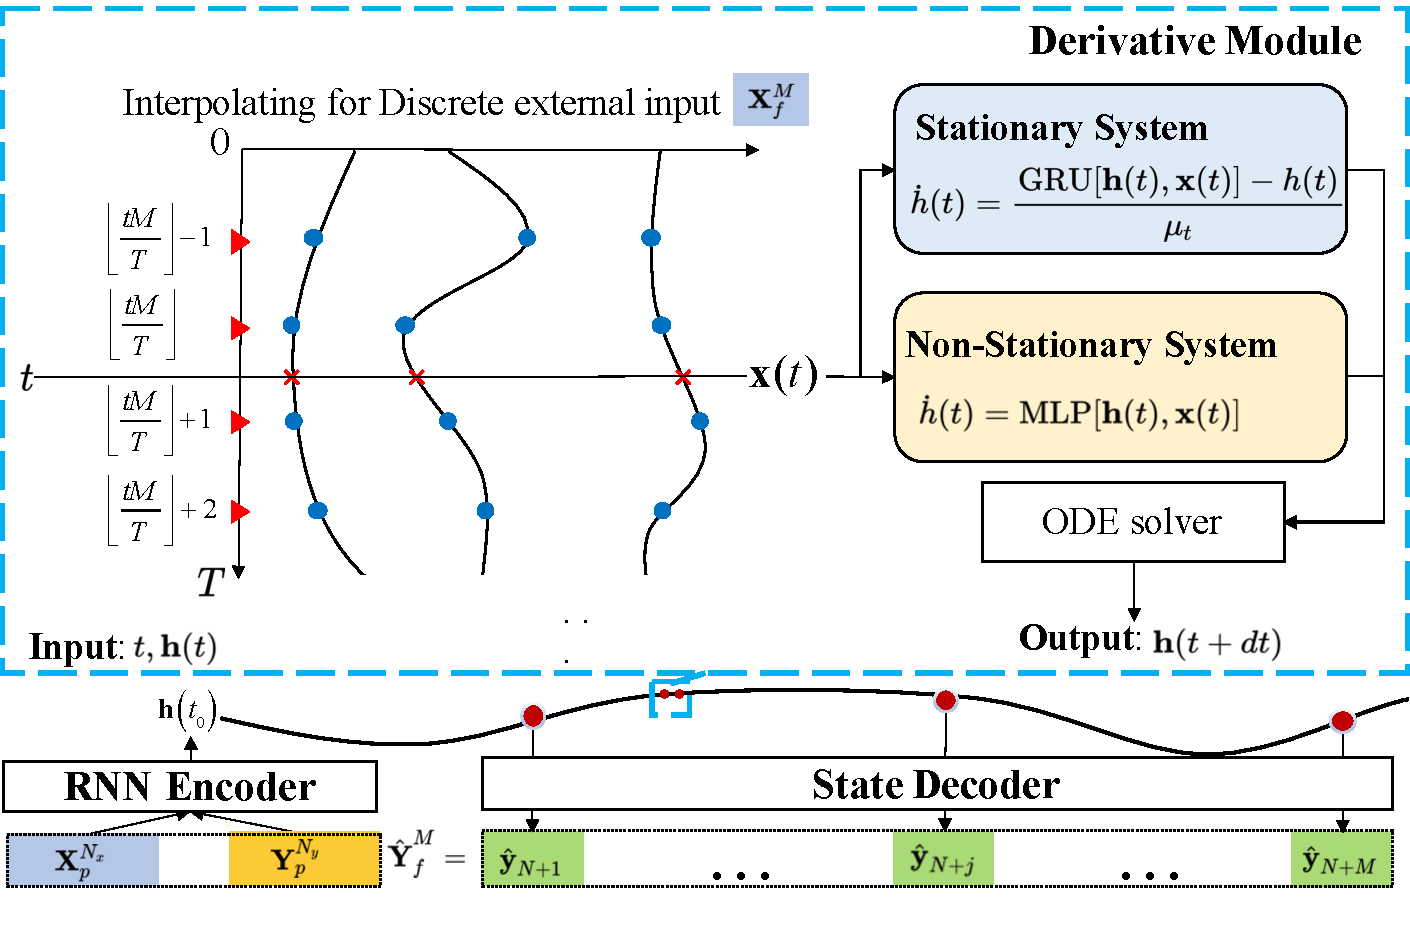
\includegraphics[width=1.0\linewidth]{figures/chapter3/model.pdf}
    \caption{
    基于ODE-net模型的输入输出系统预测模型整体结构
    % The optimized loss is defined according to accumulative errors in the complete predicted sequence. 
    }
    \label{fig:model_structure}
%\vspace*{-0.4cm}
\end{figure}

\subsection{基于循环神经网络的历史序列编码}
% In our formulation\eqref{equ:discrete_seq2seq}, the input sequences consist of three parts:
% historical system output sequence $\boldsymbol{Y}_P^{N_y})$, historical system input sequence $\boldsymbol X_p^{N_x}$ and future system input sequence $\boldsymbol X_f^{M}$. 
由于大部分工业过程具有较长的时间延迟,因此系统的历史运行轨迹数据对于模型预测极其重要。本模型引入了历史运行数据$\boldsymbol {X}_{p}^{N_{X}}$和$\boldsymbol {Y}_{p}^{N_{Y}}$作为模型输入的一部分。
具体地,利用一个基本的RNN模型,
将$\boldsymbol{Y}_p^{N_y}$和$\boldsymbol {X}_p^{N_x}$两个历史序列编码为某定长的隐状态,
以此推断常微分方程的初始值$\boldsymbol{h}(0)$ 。
\begin{equation}
\label{equ:rnn_encoder}
%\small
 \boldsymbol{h}(t_0) = \boldsymbol{h}(0) = f_{\text{RNN}}(\boldsymbol{Y}_P^{N_y},\boldsymbol X_p^{N_x},\theta _f),
\end{equation}
对于一般的工业系统,可以根据生产经验估计其系统时延为$T_d$,数据采样间隔为$T_s$,$N_y$和$N_x$可以近似估计为$N_y = N_x = N = T_d/T_s$。
% The influence of parameter $N$ on the model accuracy is examined in Section~\ref{sec:case}. 
% \begin{equation}
%     \label{NYNX}
%     N_y = N_x = T_d/T_s
% \end{equation}
在大部分工业系统中,当前系统状态与短期内的历史轨迹之间的互信息更大。
也正是因为该性质,本文利用了RNN的遗忘特性,并将其用于编码系统的历史轨迹。
利用序列编码器得到的隐状态$\b h(t_0)$编码了历史系统轨迹中对于预测所需的信息,该状态将作为待解ODE-net的初始状态。

\subsection{基于可微常微分方程网络构建系统状态空间模型}
\label{sec:ODE-net}
本小节中,我们采用参数化的连续时间状态空间模型表示系统输入、隐藏状态和输出之间的关系:
\begin{equation}
    \label{equ:ct_state_space}
%\small
     \dot{\boldsymbol h}(t)=d(\boldsymbol{h}(t), \boldsymbol{x}(t), \theta _d),
\end{equation}
\begin{equation}
\boldsymbol{y}(t)=g(\boldsymbol{h}(t)).
\end{equation}

状态空间模型能够将系统状态表示为定长的编码向量$\b h(t)$,
隐藏状态$\b h(t)$的使用对于建模长时延系统和不完全观测系统至关重要。

对于长度等于$M$的待预测序列,我们在整数离散索引$[0,1,\dots,M]$和连续时间范围$[t_0\leq t_k \leq t_{M}]$之间构造一个双射函数。
给定初始状态为$\boldsymbol{h}(t_0)$,每个$\boldsymbol{h}(t_k)$为ODE方程在$t=t_k$处的解。
为了构造一个可学习的微分系统,本章使用可微ODE-net~\cite{NIPS2018_7892}学习上述状态空间模型。

对于由某一预测评价指标确定的标量损失函数$L(\cdot)$,
其输入$\b{h}(t_k)$为ODE方程在$t=t_k$时刻的解。将ODE求解器表示为$\operatorname{ODESolve}$,我们有
\begin{align}
\label{equ:loss_ode_solver}
% \begin{aligned}
L\left(\boldsymbol{h}\left(t_{k}\right)\right)&=L\left(\boldsymbol{h}\left(t_{0}\right)+\int_{t_{0}}^{t_{k}} d(\boldsymbol{h}(t), \boldsymbol x(t), \theta_d) d t\right)\nonumber\\
&=L\left(\operatorname{ODESolve}\left(\boldsymbol{h}\left(t_{0}\right), d, t_{0}, t_{k}, \theta_d \right)\right).
% \end{aligned}
\end{align}
本文待求解的ODE方程是参数化的,
为了训练参数$\theta _d$以最小化$L(\cdot)$,我们需要根据上式计算损失函数对模型参数梯度$\partial L / \partial \theta _d$。
此处需要引入伴随状态(adjoint),即损失函数对隐状态的梯度$\boldsymbol{a}(t)=\partial L / \partial \boldsymbol{h}(t)$.

伴随状态的动态过程可由另一个ODE方程来描述,根据链式法则推导如下:
\begin{equation}
\label{equ:ode_at}
\frac{d \boldsymbol{a}(t)}{d t}=-\boldsymbol{a}^{\top}(t) \frac{\partial d(\boldsymbol{h}(t), \boldsymbol x(t), \theta_d)}{\partial \boldsymbol{h}(t)}.
\end{equation}
依赖于伴随状态,损失函数 $L(\cdot)$对参数$\theta _d$的梯度可以通过求解第三个常微分方程得到:
\begin{equation}
\label{equ:grad_ode}
\frac{\partial L}{\partial \theta _d}=-\int_{0}^{t_{M}} \boldsymbol{a}^{\top}(t) \frac{\partial d(\boldsymbol{h}(t), \boldsymbol x(t), \theta _d)}{\partial \theta_d} d t.
\end{equation}
详细的证明参见~\cite{NIPS2018_7892}.
在确定的网络结构$d$和参数$\theta _d$下,
任意的求解ODE方程的数值计算方法,如欧拉法、中点法和龙格-库塔法,均可同时求解三个微分方程,进而获得$\b h (t)$、$\alpha (t)$和${\partial L}/{\partial \theta}$在任意时刻的解。

一般情况下,在使用数值方法求解常微分方程时,具有较低误差容忍度的ODE求解器会增加调用微分函数$d$的频率。
造成更多的时间消耗,但其估计结果具有更高的准确性。
当使用神经ODE网络建模时间序列数据集时,这个准则同样是成立的。在实验环节,本章也探讨了不同微分方程求解器对于预测精度和消耗时间的影响。
时间成本和准确性的详细比较见~\ref{sec:case}节。

对于在给定时刻,ODE-net输出的的状态$\b h(t)$,需要使用状态解码器将其转换为系统的预测输出。
本文设计模型中采用的状态解码器本为全连接的网络:
\begin{equation}
    \hat{\boldsymbol y}(t) = \boldsymbol{V}^{\top} \tanh \left(\boldsymbol{W}\boldsymbol{h}_{t}+\boldsymbol{b}_{w}\right)+\b b_{v}.
\end{equation}
% A neural network with single hidden layer composed with learnable input layer ($\boldsymbol{W}$,
% $\boldsymbol{b}_w$) and hidden layer($\boldsymbol{V}$, $\boldsymbol{b_v}$) is utilized to predict the system output.
一般的状态空间模型多使用普通的矩阵变换以构建编码空间到系统输出空间的映射。本文中,由于公式
~ \eqref{equ:non_stationary}中的累加形式使输入$\b h(t)$的范围是非确定性的,而实际系统的输出空间是有界的,因此选择带有$\tanh$非线性归一化的解码器以限制解码器输出在合理的范围内。

由于模型中的编码、解码以及ODE求解过程都是可微的,本章采用标准的反向传播算法训练完整模型,损失函数定义定义为标准的均方误差损失函数:
\begin{equation}
\label{equ:mse_loss}
\mathcal{O}\left(\hat{\boldsymbol Y}^M, \boldsymbol{Y}^M\right)=\frac{1}{M} \sum_{i=1}^{M}\left|\boldsymbol y_{i}-\hat{\boldsymbol y}_{i}\right|^2.
\end{equation}

\subsection{面向不同预测时长需求的常微分方程导数模块定义}
\label{sec:derivative}
在\ref{sec:ODE-net}节中,介绍了ODE方程的求解和参数梯度的求解方法。
在本节中,将具体探讨ODE方程的参数化结构定义。
最基本的ODE-net模型采用普通的多层感知机神经网络估计状态导数\cite{chen2018neural},本文将此模型称为非平稳模型:
% We name 
% In this paper, the structures of derivative module $d$ are categorized into two types~\cite{Demeester2020SystemIW}: 
%non-stationary system or stationary system as follows:
% \begin{equation}
% \label{equ:non_stationary}
% d\left(\boldsymbol{h}(t), \boldsymbol{x}(t), \theta_{d}\right)=RNN\left(\boldsymbol{h}(t), \boldsymbol{x}(t), \theta_{d}\right)
% \end{equation}
\begin{equation}
\label{equ:non_stationary}
d\left(\boldsymbol{h}(t), \boldsymbol{x}(t), \theta_{d}\right)=\text{MLP}\left(\boldsymbol{h}(t), \boldsymbol{x}(t), \theta_{d}\right)
\end{equation}
其中$\text{MLP}(\cdot)$表示多层感知器。使用数值ODE求解方法求解非平稳系统与普通的残差网络(ResNet)有很强的相似性。

在随机过程分析领域,非平稳系统指时间序列在各点处的均值和协方差随时间变化的随机过程~\cite{GUIDOLIN2018113}。
差分操作~\cite{christoffersen2001forecasting}是一种消除序列趋势和季节性,使非平稳时间序列平稳的有效方法。
一般来说,复杂工业系统的输出往往属于非稳定时间序列,带有较强的趋势性和周期特性。
采用差分操作可以有效提高拟合精度。
在公式\eqref{equ:non_stationary}中,导数模本质上学习了隐空间中隐状态的一阶差分。
相比于ARIMA模型等直接对系统输出进行差分,面向隐状态的差分模型具有同等或更强的表示能力,以描述系统的多阶差分,进而建模更高阶的非平稳系统。

然而,非平稳系统\eqref{equ:non_stationary}在处理长期预测任务时也面临着严重的问题。
在求解长区间的ODE-net时,连续时间域内隐状态导数的不断积分会导致隐状态的取值范围显著扩增。
因此,模型的估计误差会相应增大,导致解码器难以准确地估计系统输出。

因此,本文设计了一种平稳系统作为模型的导数模块,以处理模型的长期预测问题。
具体地,其隐状态导数定义为:
%Inspired by the \emph{Differencing} operation, another architecture of derivative module named stationary system is proposed to improve the stability in long-term prediction tasks:
\begin{equation}
\label{equ:stationary}
d\left(\boldsymbol{h}(t), \boldsymbol{x}(t), \theta_{d}\right)=\frac{1}{\mu _t}(\text{GRU}\left(\boldsymbol{h}(t), \boldsymbol{x}(t), \theta_{d}\right)-\b h(t))
\end{equation}
其中$\text{GRU}$表示门控循环单元。
%Compared with differencing the system outputs directly, a model which differences the hidden states in only one-order has a strong ability to represent the high-order differencing of complicated 
% This formulation is equivalent to assume the real thickening system is a non-stationary stochastic process and learn the one-order system dynamic after differencing system hidden states.
%%%%%%%%%%%%%%%
%%%%%%%%%%%%%%
% seeking help: 随着求解长时间区间上的ODE方程, 连续累加操作可能造成隐状态数量级不断增加,进而导致隐状态估计的误差也在不断增加,这使得解码器难以将隐状态解码为正确的系统输出 
%When solving the ODE in long time range, consecutively accumulating operations extend the magnitude of hidden state $\boldsymbol{h}(t)$ significantly.
%In the meantime, unavoidably, accumulative errors in hidden state must also go up. 
%It will make decoder more difficult to decode hidden state to accurate system output.
在平稳系统中,$\text{GRU}\left(\boldsymbol{h}(t), \boldsymbol{x}(t), \theta_{d}\right)$根据当前外部输入$\b x(t)$和隐状态$\b h(t)$定义了隐状态的移动目标点。
其中,因子$\mu_t$规范了到达该目标的速度。
% No matter how long time has passed, the state $\b h(t)$ sent to decoder module is stable in the range of GRU's output.
%%%%%%%%%%
% seeking help: 举个例子,根据网络结构标准的GRU单元的输出是严格限定在(-1,1)范围内的,当h_t 向GRU的输出移动时,它不可能超过(-1, 1)这个范围。
% The standard GRU outputs the hidden state constrained in $(-1,1)$ according to the structure of network.
% The $\b h_t$ will never exceed the range of $(-1,1)$ if it moves toward the outputs of GRU.
%%%这句话我没看懂,限制的是h_t的输出范围?还是说当h_t 向GRU的输出移动时,GRU输出还是在这个范围内?
同时,由GRU网络的特性可知,其输出范围始终在$(-1,1)$中。
% It also restricts when $\b h_t$ moves toward GRU output.
无论微分方程求解时间区间范围有,隐状态$\b h (t)$将始终朝向GRU网络输出的目标值移动,因此无论微分方程求解时间区间有多大,求解ODE方程得到的任意时刻隐状态的范围都是稳定的,更便于解码器模块构建从隐空间到系统输出空间的稳定映射。
在长期预测任务中,相比于非稳定系统,这一特性能够显著地提升模型预测的稳定性。

对于平稳系统,我们主要将其用于长期预测。由于GRU具有较强的携带长时间信息的能力,所以我们使用GRU网络来构造导数模块。
对于非平稳系统中,主要将其用于短期预测。由于隐状态导数的连续累积,隐状态的变化类似于维纳过程,将会在无约束的范围内不断扩散。
而GRU、LSTM等网络均假设模型输入应限定在有界范围内。因此,本文在非稳定系统中利用MLP模块学习给定$\b h(t)$和$\b x(t)$下$\dot{\b h}(t)$的一阶导数。
\subsection{离散输入序列的可微并行插值方法}
\label{sec:interpolation}
在等式\eqref{equ:non_stationary}和\eqref{equ:stationary}中,$\dot{\b h}(t)$的计算依赖于外部输入$\b x(t)$,而训练数据中的外部输入序列$\boldsymbol X_f^M$是离散的。ODE-net的计算需要在连续时间范围内给定任意时刻的系统外部输入值$\boldsymbol x(t)$。
因此,在网络执行前向传播前,需要将离散的外部输入序列转换到连续时间域中。

在深度神经网络的训练中,通常需要利用图形处理单元(GPU)的并行计算能力,将数据批量地送入模型并进行参数更新。
因此,本章基于标准的样条插值算法,实现了一种并行样条插值机制,能够将批量输入的离散序列,并行地插值为连续时间信号。

不失一般性的,为了便于表述,我们假设系统输入的维度$m$为1。
给定以批(batch)的方式组织的输入序列为
$\b X = [\b x ^1, \b x ^2,\cdots\b x^B]$,其中$B$为批大小。
每个向量$\b x^i=x_1^i, x_2^i, x_M ^i]$
为独立的输入序列,由$M$个采样数据组成,相邻数据点之间的采样间隔是一致的。
假定与$M$个采样点相对应的求解常微分方程的时间区间为$[0,T]$。
% 对于任意给定的时间索引$T$,在这个间隔中约束为$0\leq T \leq T$。
对于任一给定的时间索引$t, 0\leq t \leq T$,我们希望并行化地估计$\b X(t) = [\b x ^1(t),\b x ^2(t),\cdot,\b x^m(t)]$。
首先构造离散下标$k=\lfloor \frac{tM}{T} \rfloor$,给定$n+1$个数据点,$\{(k, \b x_k),(k+1, \b x_{k+1}),\cdots,(k+n, \b x_{k+n})\}$
可以计算$n$阶样条插值函数的系数矩阵$\b A\in\mathbb{R}^{(n+1)\times m}$:

% 首先,在区间$[0,t]$中,找到最接近$t$的且在$\{1,\cdots,M\}$中出现的整数索引$k=\lfloor \frac{tM}{T} \rfloor$。
\begin{equation}
\boldsymbol{A}=\left[\begin{array}{ccc}
k^{0} & \cdots & k^{n} \\
(k+1)^0 & \cdots & (k+1)^{n} \\
\vdots & \ddots & \vdots \\
(k+n)^0 & \cdots & (k+n)^{n}
\end{array}\right]^{-1}\left[\begin{array}{ccc}
x_{k}^{1} & \cdots & x_{k}^{m} \\
x_{k+1}^{1} & \cdots & x_{k+1}^{m} \\
\vdots & \ddots & \vdots \\
x_{k+n}^{1} & \cdots & x_{k+n}^{m}
\end{array}\right].
\end{equation}
一批数据中,所有离散序列在$t$时刻的插值结果如下:
\begin{equation}
\left[\b x^1(t),\b x^2(t),\cdots,\b x^m(t)\right]= \Bigg(\left[ 1, \frac{tM}{T},\cdots, (\frac{tM}{T})^n\right]\boldsymbol{A}\Bigg). 
\end{equation}
在一般的深度学习框架中,上述矩阵乘法和求逆矩操作可以高效地并行实现。
% For uneven case, the interval time for sampled data is not constant.
% An obvious way is employing any interpolation method to pad the original data and produce a sequence with even time separation before training.
% Furthermore, some frequency domain based method could also produce continuous-time sequence from the discrete. 
% But we did not employ such methods because these methods only reserve the low frequent information and destroy the original sequence on discrete integral points.
% %and produce a new one.
% For example, the butterworth filter, a kind of low pass filer, will produce $x(t)\neq x_i$ when $\frac{tM}{T}=i$. 
% While the spline interpolations can avoid this problem.
% The experiment section will show the influence from the choice of the order in spline interpolation.

\section{基于工业数据集的模型性能分析}
\label{sec:case}

\begin{figure}[t]
%\setlength{\abovecaptionskip}{-0.1cm} 
\centering
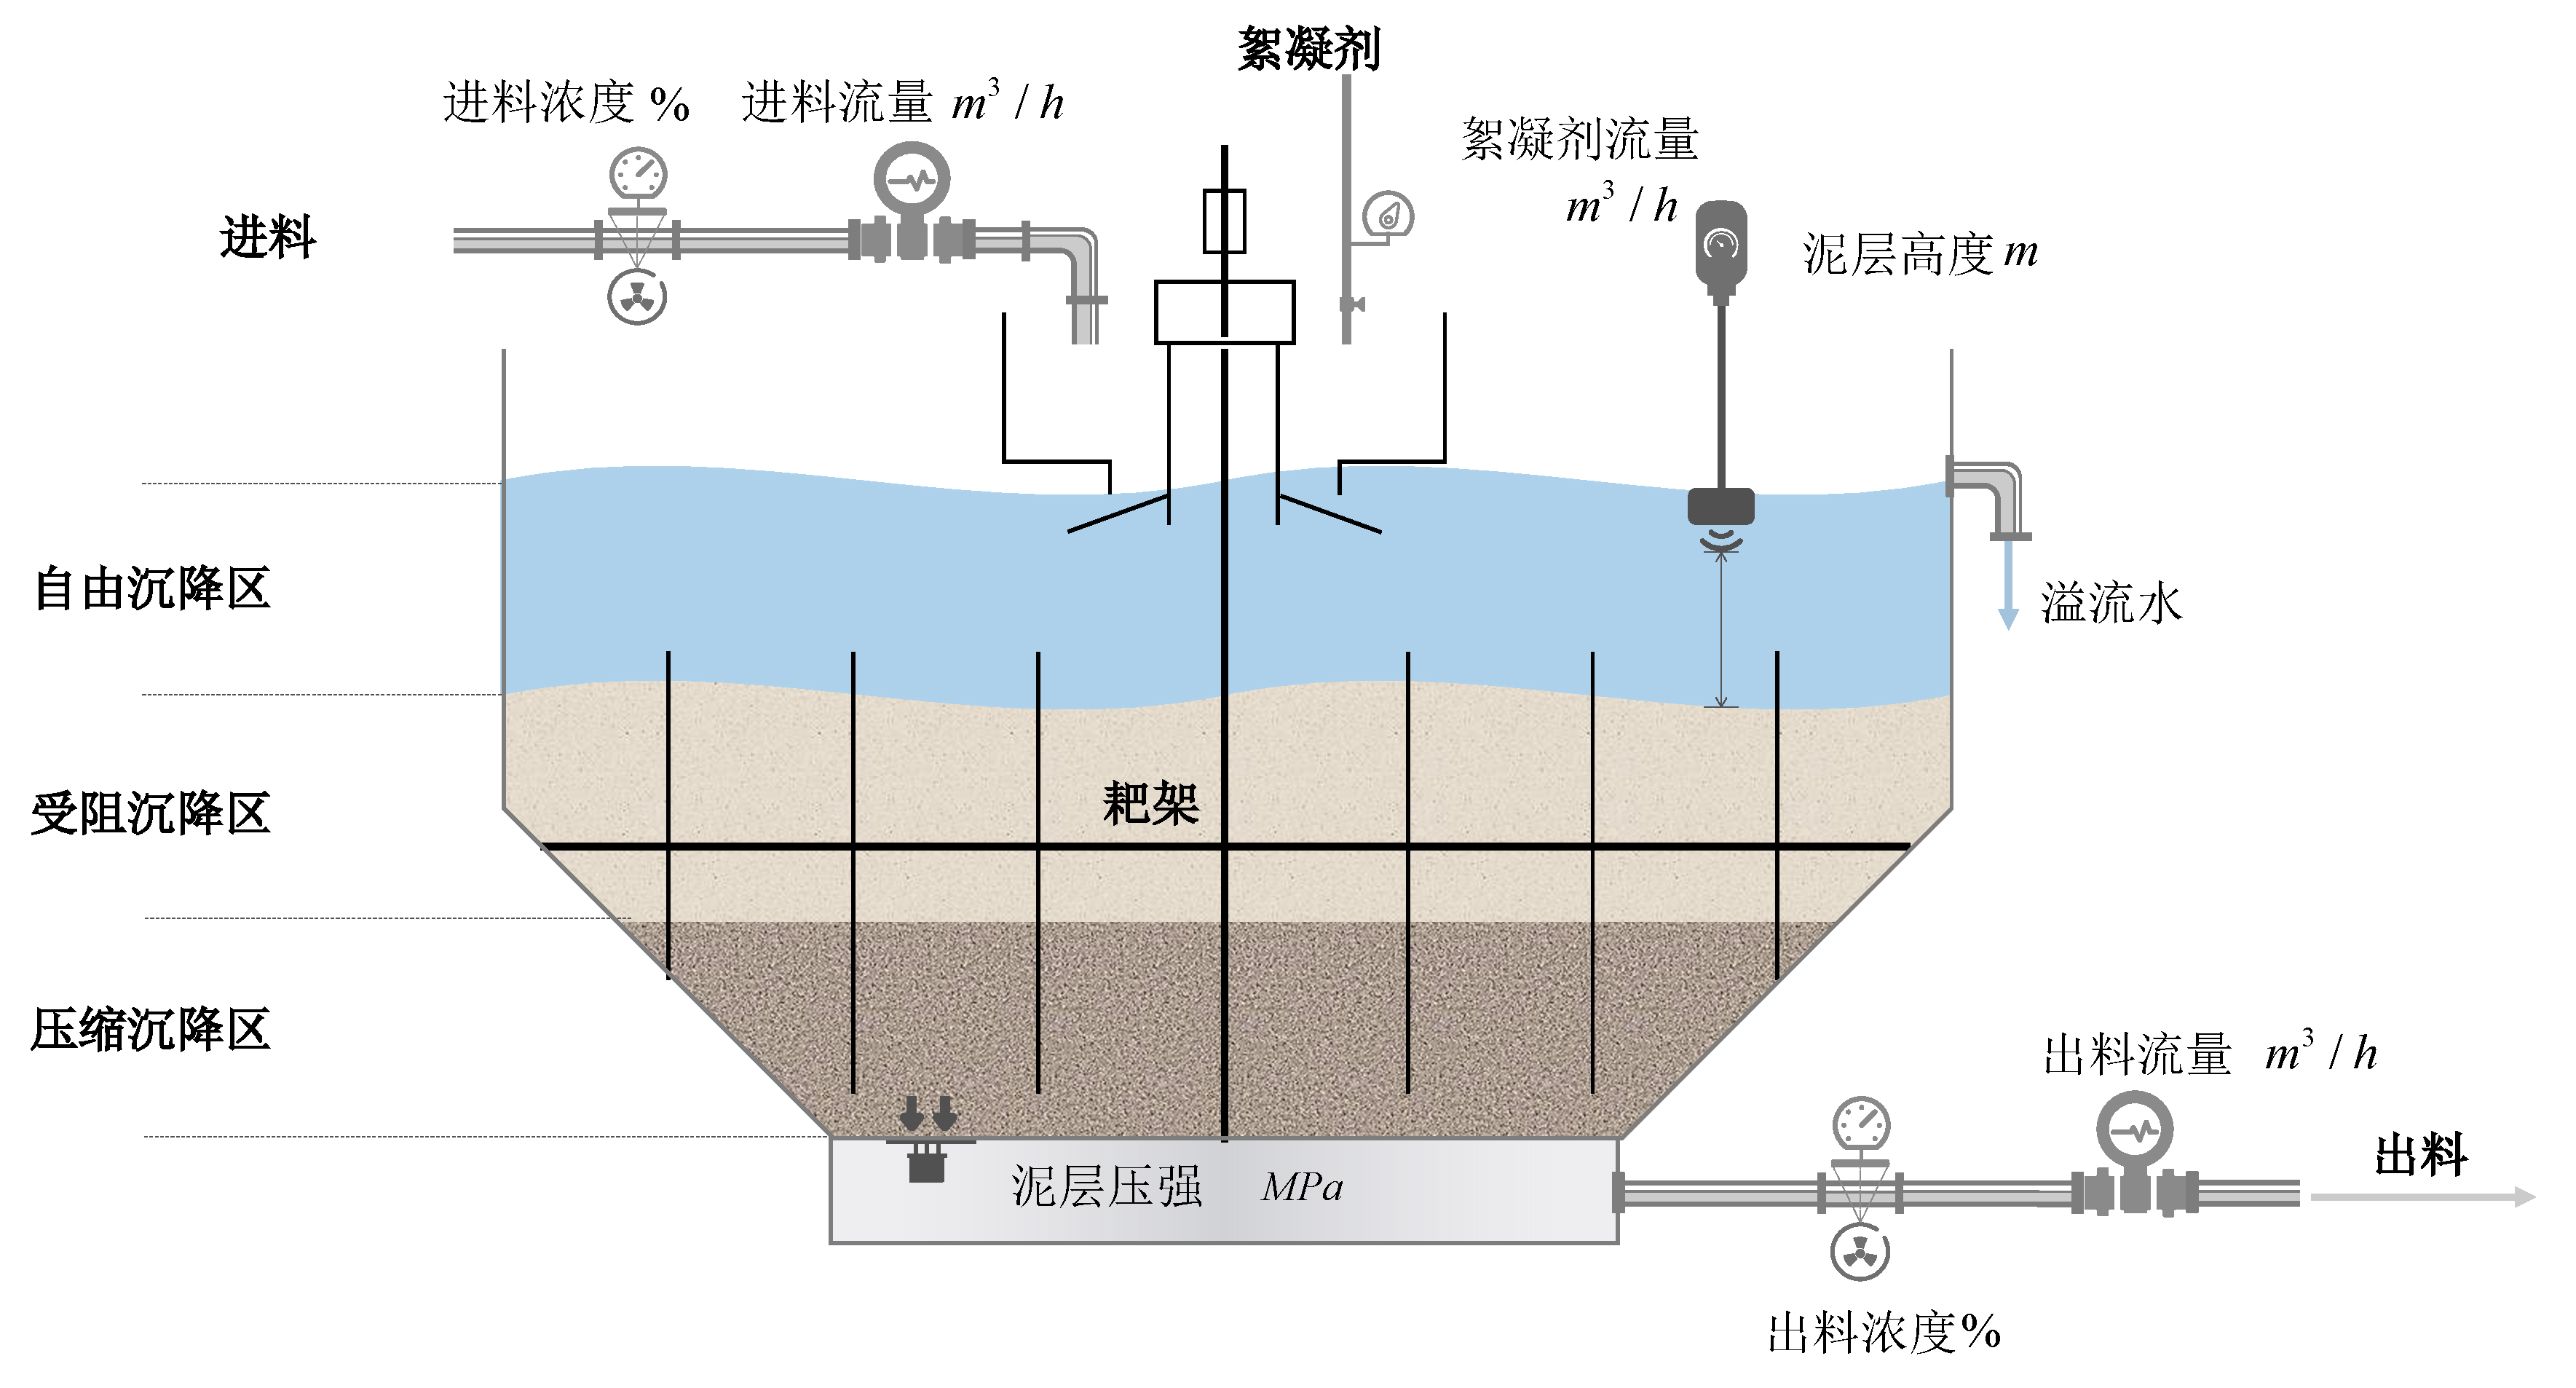
\includegraphics[width=\linewidth]{figures/chapter3/thickener.pdf}
\caption{
%%%%%%%%%%%%%%%%%%%%%%%%%%%
% seeking help: 如图所示,在实验的充填站,共有两台深锥浓密机,其中一主用,一备用,本文实验数据全部来源于第一台主用设备。
%As the figures illustrate above, there are two identical paste thickeners in the experimental backfilling station. One of them is primary device and the other is a spare. All of the original dataset in experiments are exported from the primary one.
膏体浓密机系统运行过程及监测变量图示
% The training data we use in this paper is collected from the primary device.
}
%%%%%%%%%%%%%%%%%%%%%%%%%%%
\label{fig:nfca_thickener}
%\vspace*{-0.3cm}
\end{figure}

% This section presents experimental results for the proposed method on the dataset of real thickening systems.
本节给出了所述方法在真实膏体浓密机系统数据集上的预测实验结果。
实验只要探究三个问题:

\textbf{问题1}:相比于直接采用离散时序预测模型,使用深度连续时间网络和高精度ODE求解器建模预测工业系统能否获得更优的效果?

\textbf{问题2}:在预测任务中使用平稳系统和非平稳系统的优缺点是什么?

\textbf{问题3}: 不同的插值方法和序列编码器的编码长度会如何影响所提出的CT模型的准确性?
本节中,我们将首先介绍数据集、模型超参数以及训练和测试参数的配置。然后给出详细的实验结果。

\subsection{膏体浓密机系统数据集}
\label{sec:paste_introduction}
在实验环节中,本章所用的工业系统数据来自于赞比亚铜带省,NFCA非洲矿业有限公司的膏体浓密机。
该设备由FLSmidth公司生产。
如图~\ref{fig:nfca_thickener}所示。该设备用于在膏体充填站将铜尾矿浓缩成高浓度料浆以用于充填膏体的制备。
两台设备都运行在闭环PID控制模式下。
% The dataset includes some key parameters in paste thickener which are listed in Table~\ref{tab:monitor_points}.
% \begin{table*}[htpb]
% \caption{Detailed monitoring point list in thickener system}
% \label{tab:monitor_points}
% \centering
% %% \tablesize{} %% You can specify the fontsize here, e.g., \tablesize{\footnotesize}. If commented out \small will be used.
% \begin{tabular}{cccc}
% \toprule
% \textbf{Name} & \textbf{Symbol} & \textbf{Unit}	& \textbf{Point description}\\
% \midrule
% 	Feed flow rate 	& $x^0$			& $m^3/h$ & Flow speed of the feed with low concentration \\
% 	Feed concentration 	& $x^1$			& $\%$ & Concentration of the Feed flow \\
% 	Mud Pressure	& $y^0$			& $MPa$ & Mud pressure at the bottom of the tank\\
% 	Rake speed & $x^2$ & rpm & Rotating speed of rake in thickener \\
% 	Flocculant flow rate	& $x^3$			& $m^3/h$ & Dosage of the flocculant\\
% 	Underflow rate	& $x^4$			& $m^3/h$ & Flow speed of the discharged underflow\\
% 	Underflow concentration	& $y^1$			& $\%$ & Concentration of the discharged underflow \\
% \bottomrule
% \end{tabular}
% \end{table*}
实验所用全部数据采集于2018年5月到2019年2月,采集间隔为两分钟。表~\ref{tab:dataset}展示了部分数据。
\begin{table*}[ht]
\small
\centering
\caption{膏体浓密机系统数据样例}
\label{tab:dataset}
\resizebox{0.9\linewidth}{!}{
\begin{tabular}{cccccccc}
\toprule
 采集时间      & \begin{tabular}[c]{@{}c@{}}进料 \\ 流量\end{tabular} & \begin{tabular}[c]{@{}c@{}}进料 \\ 浓度\end{tabular} & \begin{tabular}[c]{@{}c@{}}泥层 \\ 压力\end{tabular} & \begin{tabular}[c]{@{}c@{}}耙架 \\ 转速\end{tabular} & \begin{tabular}[c]{@{}c@{}}底流 \\ 流速\end{tabular} & \begin{tabular}[c]{@{}c@{}}底流 \\ 浓度\end{tabular} & \begin{tabular}[c]{@{}c@{}}絮凝剂\\ 流速\end{tabular} \\ \hline
2018/5/9 10:20  & 164.47                                                    & 16.47                                                         & 18.41                                                   & 500.58                                                                                                                                                  & 58.96                                                     & 59.72                                  &4.30                          \\
2018/5/9 10:22 &169.21                                                   & 15.51                                                         & 17.99                                                   & 500.16                                                                                                                                                  & 61.56                                                     & 58.88                                     &4.06                        \\ 
2018/5/9 10:24 & 141.78                                                    & 15.30                                                         & 16.41                                                   & 500.56                                                                                                                                                  & 59.97                                                     & 59.26                                   &4.06                          \\
2018/5/9 10:26 & 305.67                                                    & 25.31                                                         & 16.11                                                   & 500.99                                                                                                                                                  & 59.46                                                     & 58.77                                   &4.07                          \\
2018/5/9 10:28 & 328.70                                                    & 28.28                                                         & 16.43                                                   & 501.42                                                                                                                                                  & 59.68                                                     & 59.43                                   &4.43                          \\
2018/5/9 10:30 & 323.96                                                    & 25.90                                                         & 17.11                                                   & 501.56                                                                                                                                                  & 61.40                                                     & 60.09                                   &4.40                          \\
\bottomrule
\end{tabular}}
\end{table*}
收集的数据集来自于7个监测传感器,
系统输出变量$\b y(k) \in \mathbb{R}^2$中,包括底流浓度$y_1(k)$和泥层压力$y_2(k)$。
$y_1(k)$和$y_2(k)$均受到控制输入$\b x(k)\in \mathbb{R}^5$影响,包括进料流量$u_1(k)$、进料浓度$u_2(k)$、耙架转速$u_3(k)$、底流流量$u_4(k)$和絮凝剂流量$u_5(k)$。
删除系统停机时的异常监测数据,累计剩余24,673条数据。

本节采用滑动窗口法生成训练及测试样本对$(\b X _p^N, \b Y _p^N, \b X _f^M, \b Y _f^M)$,。
具体地,原始数据集依照浓密机系统的启停时间,分为多个文件。每个文件包含了连续生产过程中7个传感器的监测数据序列,且各序列中数据点的采样间隔均为2分钟。
对于每个文件中的多个序列,将大小为$N+M$的滑动窗口沿着序列的时间维度正向移动,移动步长为1。
% 为了从中的多个数据序列构建样本对$(\b X _p^N, \b Y _p^N, \b X _f^M, \b Y _f^M)$,
当窗口到达$i$位置时,四个序列$(\b X _p^N =\b X[i:i+N]$, $\b Y _p^N =\b Y[i:i+N]$, $\b X _f^M=\b X[i+N:i+N+M]$, $\b Y _f^M=\b Y[i+N:i+N+M])$被收集作为训练或测试样本。

%%%%%%%%%%%%%
% seeking help: 理想情况下,让滑动窗口的移动距离等于$N+M$ 是最佳的选择,这样可以保证任何两个训练数据对之间不存在交叉
%Ideally, it is the best choice that setting moving steps of sliding window equals to $N+M$ which keep no intersection of any two pieces.
% Ideally, it is the best choice to set the moving steps of the sliding window to $N+M$. This can guarantee that there is no intersection of any training data.
%%%%%%%%%%%%%
% However, when the total length of the original data from a thickening system is $|S|$, the remaining data groups count only $\frac{|S|}{N+M}$, which is not sufficient to train our complex model.
在验证集和测试集数据中,滑动窗口的大小设置为$N+L$,其中$L$表示待预测序列的长度(可能不等于训练集中待预测序列的长度$M$)。
模型仅通过训练集数据进行训练,然后使用不同的$L$在不同的验证集和测试集数据上进行验证和评估。
% The detailed parameters will be introduced in experimental paragraph.
% The detailed procedure for constructing datasets is illustrated in Fig.~\ref{fig:dataset}.
构造数据集的详细过程如图~\ref{fig:dataset}所示。
\begin{figure}[t]
    \centering
    %\vspace{-5pt}
    %\setlength{\abovecaptionskip}{-0.1cm} 
    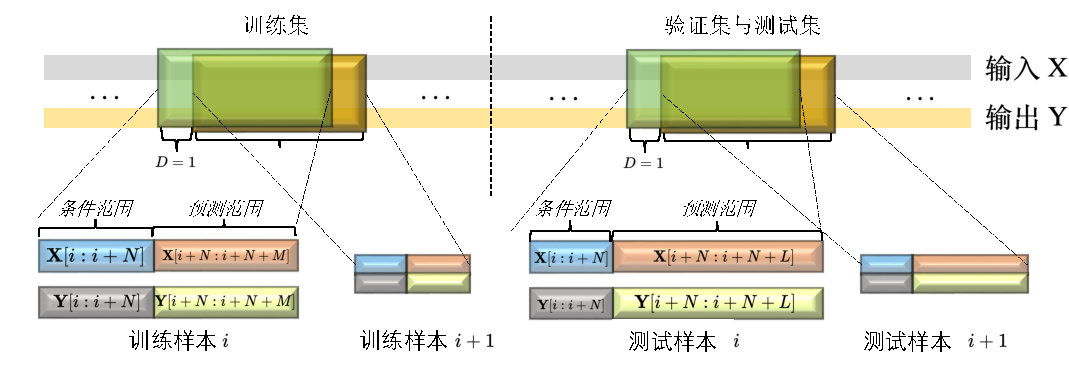
\includegraphics[width=\linewidth]{figures/chapter3/dataset.pdf}
    \caption{
    % Training set is built by moving a sliding window with speed $2$. Validation set and test set are built by moving a sliding window with speed $N+L$. $N$ is the length of encoded historical sequence. M is the length of predicted sequence in training phase. L is the length of predicted sequence in test or validation phase and it is a variable in different experiments.
    训练集、验证集、测试集的构建过程图示
    }
    \label{fig:dataset}
%\vspace*{-0.4cm}
\end{figure}

本节使用数据集的前$70\%$用于模型训练。在剩下的$30\%$中,前$15\%$作为验证集,帮助确定最佳训练轮次,剩下的$15\%$作为测试数据集用于评估模型准确性。
训练时,历史序列的长度为$N=80$,预测序列长度为$M=60$。
测试环节探究了$L=60, 200, 500$三种情况下,模型的预测性能。
根据图~\ref{fig:dataset}所示的构建输入-输出序列对的方法,共计17131个样本对用于训练。对于不同预测长度$L=60、200、500$,分别有3561、3421、3121个样本对用于测试和验证。
所有的数据在训练和测试之前均被归一化为标准正态分布。




\subsection{实验设定}

实验中,使用mini-batch随机梯度下降(SGD)和Adam优化器\cite{kingma2014adam}对模型进行训练。
batch size为$512$,学习速率为$0.001$,并且呈指数衰减。
衰减率为$0.95$,衰减周期为10个训练轮次。
ODE-net中隐藏状态$\b h(t)$的大小为$32$。
RNN序列编码器模块包含一个隐藏层,隐状态大小等于$32$,这隐状态$\boldsymbol h(t)$的大小一致。
状态解码器中隐藏层的大小为$64$。
在设定自适应微分方程求解器参数时,由于降低近似误差的容忍度,会导致求解常微分方程的时间剧烈增加。
在所有的实验中,为了平衡时间消耗和预测精度,我们将所有ODE求解器容忍的最大相对误差设置为$1\mathrm{e}-4$,容忍的最大绝对误差设置为$1\mathrm{e}-5$。
训练时,找到在验证集上预测精度最高的模型,将其用于测试数据集精度评估。
训练和测试均在单个Nvidia V100 GPU上进行。
代码基于PyTorch框架实现。
对于给定的离散整数下标序列$[0,1,\dots, M]$, 我们定义其连续时间区间为 $0\leq t\leq M\delta_t$.
相邻数据点的时间间隔$\delta _t$被设置为0.1。
因此,公式\eqref{equ:stationary}中的归一化因子$\mu _t$也被设置为0.1。
当使用欧拉数值求解器求解稳定系统的ODE方程时,模型将等价于使用GRU单元在离散时间系统下进行预测:
% \begin{equation}
\begin{align}
    \b h(t+\delta _t) &=\b h(t) + \delta _t \cdot \frac{\text{GRU}\big(\b h(t),x(t), \theta_d \big) - \b h(t)}{\mu _t}  \nonumber\\
                      &= \text{GRU}\big(\b h(t),x(t), \theta _d\big).
\end{align}
% \end{equation}

本节使用模型预测底流浓度的平均根相对平方误差(RRSE)和平均平方误差(MSE)评价不同模型的预测精度。
对于预测长度$L$,RRSE定义如下:
\begin{equation}
\begin{aligned}
    \text{RRSE}=\sqrt{\sum_{j=1}^{L} \frac{e_{j}^{2}}{\left(\hat{y}_{j}-\bar{y}\right)^{2}}}, \quad e_{j}=\hat{y}_{j}-y_{j}.
\end{aligned}
\label{equ:rrse}
\end{equation}
RRSE可以解释为被归一化的均方根(RMS)误差。

% \subsection{实验结果分析与讨论}

% To demonstrate the significance of proposed continuous-time system identification model.
% We construct two kinds of competitive baselines for substituting derivative module:
% \begin{equation}
%     \label{equ:nodiff_rnn}
%     \boldsymbol{h}(i+1)=R(\boldsymbol{h}(i), \boldsymbol{x}(i))
% \end{equation}
% \begin{equation}
%     \label{equ:diff_rnn}
%     \boldsymbol{h}(i+1)=R(\boldsymbol{h}(i), \boldsymbol{x}(i)) + \epsilon \boldsymbol{h}(i)
% \end{equation}
% Model with structure \eqref{equ:nodiff_rnn} is basic recurrent neural networks model which can be used to learn time series model and stationary system.

\subsection{不同模型预测结果对比}
首先,我们研究了不同ODE求解器和导数模块对预测精度的影响。
我们选择了四个ODE求解器:Euler, midpoint,四阶Runge—Kutta (RK4), Dormand—Prince (Dopri5)\cite{NIPS2018_7892},以及三阶Bogacki—Shampine(Bosh)\cite{bogacki19893}。我们研究了这些微分方程求解器结合非稳定和稳定系统时的性能。
此外,我们还对比了离散时间深度序列模型,包括状态空间(DT-State-Space)、基于注意力机制的Seq2Seq模型(Attention-Seq2Seq)\cite{Member2019}和Transformer模型\cite{Wu2020}。
DT-State-Space~\cite{Rangapuram2018}模型采用循环神经网络(RNN)建模线性状态空间模型的参数,并基于预测得到的状态空间模型预测时间序列。其状态空间和RNN隐藏层的大小分别设置为16和32。
Transformer和Attention-Seq2Seq的超参数设置与原文献保持一致。

我们进行了三组实验以探究不同预测长度$L=60$、$200$和$500$下,不同模型预测结果的RRSE、MSE和预测速度。
% Table~\ref{tab:exp_all} presents the results of the predicted underflow concentrations. 
\begin{table*}[htpb]
%\setlength{\abovecaptionskip}{-0.1cm} 
\caption{
%%%%%%%
% seeking help : 预测底流浓度的RRSE、MSE 误差 以及每次预测序列所需的时间
%RRSE and MSE error of predicted underflow concentration and time consumption for each prediction.
Root relative squared error (RRSE), mean squared error (MSE), and time consumption of predicted underflow concentration.
}
%%%%%%%
\label{tab:exp_all}
\centering
% \setlength{\tabcolsep}{3.0mm}{%7可随机设置,调整到适合自己的大小为止
\resizebox{\linewidth}{!}{
\footnotesize
\renewcommand{\arraystretch}{1.5}
\begin{tabular}{c|c|ccccccccc}
\toprule
\multicolumn{2}{c|}{\multirow{2}{*}{模型}}                                                                        & \multicolumn{3}{c|}{$L=60$}                                                           & \multicolumn{3}{c|}{$L=200$}                                                           & \multicolumn{3}{c}{$L=500$}                                         \\ \cline{3-11} 
\multicolumn{2}{c|}{}                                                                                              & RRSE                 & MSE                  & \multicolumn{1}{c|}{Time (s)}             & RRSE                 & MSE                  & \multicolumn{1}{c|}{Time (s)}              & RRSE                 & MSE                  & Time (s)                \\ \hline
\multirow{4}{*}{\begin{tabular}[c]{@{}c@{}}非稳定\\ 系统\end{tabular}} & \multicolumn{1}{c|}{Euler}     & 3.18                 & 9.07                 & \multicolumn{1}{c|}{1.71}             & 5.09                 & 80.25                & \multicolumn{1}{c|}{3.81}              & 3.95                 & 152.21               & 4.65                 \\
                                                                                 & \multicolumn{1}{c|}{Mid-Point} & 3.10                 & 8.95                 & \multicolumn{1}{c|}{3.23}             & 5.24                 & 80.29                & \multicolumn{1}{c|}{7.36}              & 4.16                 & 172.43               & 9.15                 \\
                                                                                 & \multicolumn{1}{c|}{RK4}       & 3.10                 & 8.97                 & \multicolumn{1}{c|}{6.95}             & 5.24                 & 83.90                & \multicolumn{1}{c|}{14.82}             & 4.16                 & 172.64               & 18.76                \\
                                                                                 & \multicolumn{1}{c|}{Bosh}    & 3.08  & 8.57  & \multicolumn{1}{c|}{12.8}             & 5.84                 & 84.60                & \multicolumn{1}{c|}{19.0}              & 4.61                 & 172.39               & 24.75                \\
                                                                                 & \multicolumn{1}{c|}{Dopri5}    &  \uline{\textbf{2.83}}  &  \uline{\textbf{6.40}}  & \multicolumn{1}{c|}{9.63}             & 5.31                 & 84.60                & \multicolumn{1}{c|}{13.8}              & 4.19                 & 175.39               & 25.75                \\ \hline
\multirow{4}{*}{\begin{tabular}[c]{@{}c@{}}稳定\\ 系统\end{tabular}}     & \multicolumn{1}{c|}{Euler}     & 3.18                 & 9.06                 & \multicolumn{1}{c|}{1.63}             & 3.75                 & 34.78                & \multicolumn{1}{c|}{3.58}              & 1.63                 & 37.77                & 4.66                 \\
                                                                                 & \multicolumn{1}{c|}{Mid-Point} & 3.18                 & 9.08                 & \multicolumn{1}{c|}{3.22}             & 3.73                 & 34.64                & \multicolumn{1}{c|}{7.17}              & 1.62                 & 38.36                & 9.3                  \\
                                                                                 & \multicolumn{1}{c|}{RK4}       & 3.18                 & 8.96                 & \multicolumn{1}{c|}{6.80}             &  \uline{\textbf{3.58}}  &  \uline{\textbf{32.90}} & \multicolumn{1}{c|}{15.17}             &  \uline{\textbf{1.61}}  &  \uline{\textbf{34.88}} & 18.66                \\
                                                                                 & \multicolumn{1}{c|}{Bosh}    & N/A                    & N/A                    & \multicolumn{1}{c|}{\textgreater{}50} & N/A                    & N/A                    & \multicolumn{1}{c|}{\textgreater{}200} & N/A                    & N/A                    & \textgreater{}3000   \\
                                                                                 & \multicolumn{1}{c|}{Dopri5}    & N/A                    & N/A                    & \multicolumn{1}{c|}{\textgreater{}50} & N/A                    & N/A                    & \multicolumn{1}{c|}{\textgreater{}200} & N/A                    & N/A                    & \textgreater{}3000   \\ \hline
\multicolumn{2}{c|}{Attention-Seq2Seq\cite{Member2019}}                                                                             & 3.13                 & 8.97                 & \multicolumn{1}{c|}{0.41}             & 4.02                 & 33.90                & \multicolumn{1}{c|}{0.41}              & 1.82                 & 40.53                & 0.42                 \\ \hline
\multicolumn{2}{c|}{DT-State-Space\cite{Rangapuram2018}}                                                                               & 3.22                 & 9.36                 & \multicolumn{1}{c|}{0.06}             & 4.69                 & 41.11                & \multicolumn{1}{c|}{0.07}              & 3.35                 & 45.64                & 0.08                 \\
\multicolumn{2}{c|}{Transformer\cite{Wu2020}}                                                                               & 3.16                 & 8.36                 & \multicolumn{1}{c|}{0.02}             & 3.99                 & 40.23                & \multicolumn{1}{c|}{0.02}              & 2.55                 & 44.23                & 0.03                 \\
\bottomrule
\end{tabular}}
\end{table*}

在表~\ref{tab:exp_all}中可以发现,离散时间域下的Attention-Seq2Seq模型、DT-State-Space模型和Transformer的性能稍优于使用Euler求解器的模型效果,但差于使用高阶ODE求解器获得的预测效果,特别是在长期预测$L=200, 500$时表现更为明显。
结果表明,采用连续时间模型可以更好地反映浓密机系统的连续时间演化特征,从而相比于纯离散时间模型,呈现更高的预测精度。

\subsection{不同ODE求解器对比}
进一步地,我们分别对采用了不同ODE求解器的稳定系统模型和非稳定系统模型进行分析比较。

当导数模块被定义为非稳定系统时,对于短期预测任务$L = 60$,
我们发现,虽然Euler求解器的时间消耗低于其他ODE求解器,但其预测结果的RRSE和MSE指标较高,预测精度差于使用其他四个ODE求解器。
原因在于欧拉方法作为求解ODE方程最简单的方法,它在两个相邻时间点之间仅仅调用导数模块计算隐状态的一阶导数一次,然后计算状态差分。其运行本质等同于离散时间序列模型,算得ODE方程的解的精度较差,并没有充分利用模型为连续时间系统的性质。
相应地,中值法和4阶Runge-Kutta法在两个相邻时间点之间,分别调用了导数模块计算隐状态导数2次和4次。因此,其对隐状态轨迹的求解精度高于欧拉法。
该结果也证实了,基于Euler方法的离散时间序列模型忽略了系统的连续时间特性,因此不能精确地学习系统的动态过程。
进一步地,作为隶属于龙格-库塔体系中的常微分方程自适应步长求解方法,Dopri5和Bosh方法能够确保数值近似解与真实解之间的误差限定在指定误差范围内。
随着给定误差限的缩小,求解ODE方程的时间消耗也随之增加。
虽然两种方法求解ODE耗时较长,但精度较高。Dopri5的预测性能稍好于Bosh。

%It is also equivalent to standard discrete-time deep sequential model which is the most common choice for formulating an evenly sampled dynamical system.

% 当导数模块分别被定义为非稳定系统与稳定系统时,ODE求解器在预测精度和时间消耗上表现也会收到
% 实验中,我们还发现,同一ODE求解器在预测精度和时间消耗上表现也会受到导数模块定义的影响。
当导数模块定义为平稳系统时。
两种自适应方法Bosh和Dopri5求解ODE方程的时间消耗将显著增加。
在表\ref{tab:exp_all}中,我们没有列出Dopri5和Bosh在稳定系统中的预测精度,因为其计算速度极慢,使得该方法不适用于实际工业应用。
对比其他ODE求解器,我们发现RK4等高阶ODE求解器的求解误差小于低阶ODE求解器,但在求解ODE方程时需要消耗更多的时间。


%are relatively higher order ODE solvers which have higher accuracy than Euler and evaluate the derivative network for 2 times and 4 times respectively between two adjacent time points. As an adaptive method in Runge–Kutta family, Dopri5 ensures that the output is within a given tolerance of true solution.
% while the decrease of tolerance is accompanied by the increases of times for evaluating the differential equation.
%%%%%%%%%%%%%%%%
% seeking help: 在Dopri5中,求解ODE的时间会伴随着减少误差容许度而增加,我们在实验中将相对容许度设置为1e-4, 绝对容许度设置为1e-5.
%In Dopri5, the time for evaluating the differential equation will increase if we reduce the tolerance of calculation error. 
%In all of experiments, we set the relative tolerance to $1e-4$ and absolute tolerance to $1e-5$.

% According to our industrial requirement from the system, we set the relative tolerance to $1e-4$ and absolute tolerance to $1e-5$.

%%%%%%%%%%%%%%%%
% The definition of $RNN$ in \eqref{equ:non_stationary} and \eqref{equ:stationary} varies from basic RNN to GRU, ASRNN and and simple (Multi-Layer Perceptron, MLP).


% The form \eqref{equ:diff_rnn} adds a skip connection based on original RNN which can be interpreted as Euler approximation of ODE-net model. 
% $epsilon$, an experimental parameter, is set to $0.1$ to restrain the fluctuation of hidden state.
% Under the assumption of continuous-time property in thickening system, form \eqref{equ:diff_rnn} is considered to perform better than \eqref{equ:nodiff_rnn} in theory.
% In our experiment, RNN, LSTM, GRU, ASRNN are original sequential models with structure \eqref{equ:nodiff_rnn}, 
% and the identifiers RNN-Diff, LSTM-Diff, GRU-Diff, ASRNN-Diff represent the networks with skip connection \eqref{equ:diff_rnn}. 
% These discrete-time models depends on the data are sampled evenly which is satisfied in our experiment, 

% A closer model with ODE-net is Runge-Kutta neural network~\cite{Wang1998} which is a approximation of continuous-time model.
% We set the order of Runge-Kutta network as 4 and the output is described by:
% A thorough experiment in Tab.\ref{tab:exp_all} is conducted to study the influence from ODE solver and system dynamic to prediction accuracy and time cost. 
% In Tab.\ref{tab:exp_all}, only the metrics on underflow concentration are listed in the table because underflow concentration is generally more noteworthy than mud pressure in thickening system.
%For the experiments with $L=60$ as shown in Table~\ref{tab:exp_all}, the length of predicted sequence is relatively shorter than other experimental groups.


% \paragraph{Comparison of stationary models and non-stationary models}
\subsection{稳定系统与非稳定系统对比}

为了更直观地比较使用稳定系统和非平稳系统定义导数模块的区别,我们进一步地可视化了不同ODE求解器对非稳定和稳定系统的预测效果。
图\ref{fig:predict_cmp_60}描述了对于$L=60$的短期预测任务,使用不同ODE求解器求解非平稳系统和平稳系统得到的预测序列:
\begin{figure}[h]
\centering
%\setlength{\abovecaptionskip}{-0.1cm} 
\subfigure[稳定系统+RK4求解器]{
\begin{minipage}[t]{0.33\linewidth}
\centering
% \hspace{-22pt}
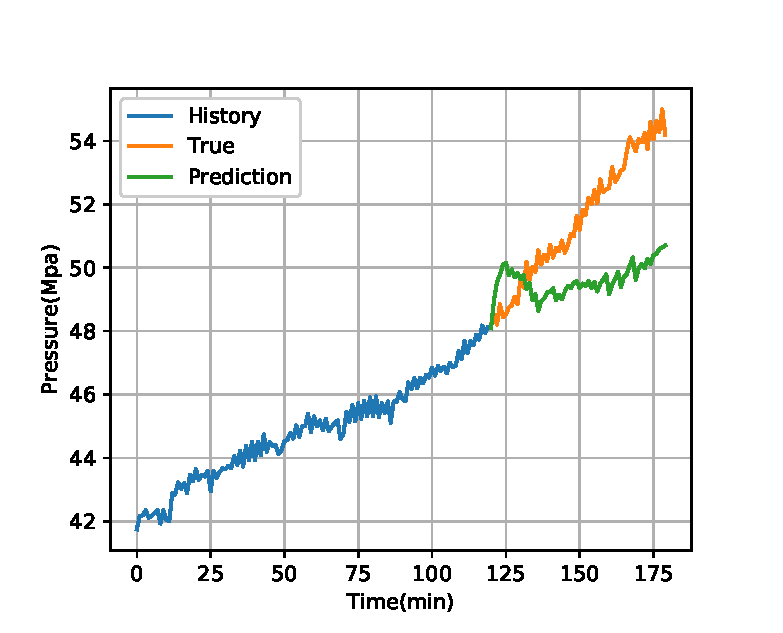
\includegraphics[width=\linewidth,trim=12 0 0 20,clip]{figures/chapter3/predict_cmp/Pressure_GRU_sta_rk4_60.eps}
% \hspace{-18pt}

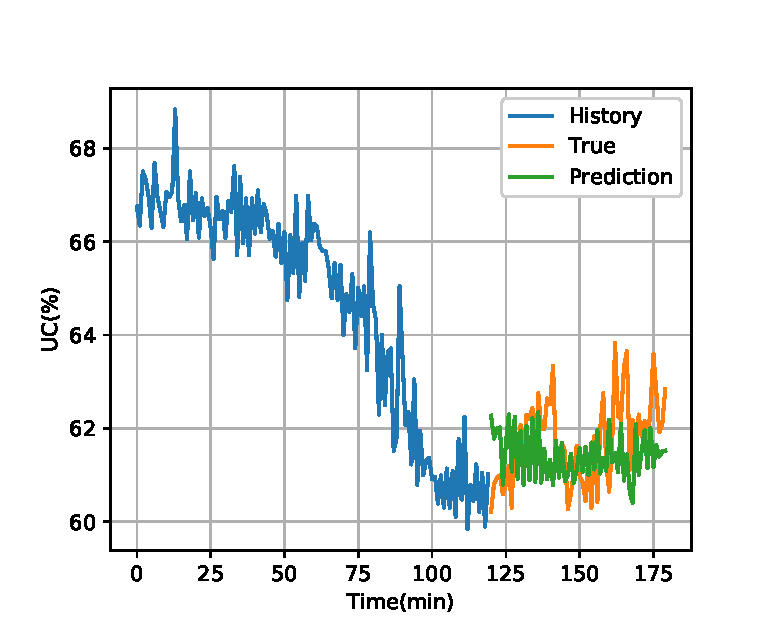
\includegraphics[width=\linewidth,trim=12 0 0 20,clip]{figures/chapter3/predict_cmp/UC_GRU_sta_rk4_60.eps}
%\caption{fig1}
\end{minipage}
}%
\hspace{-22pt}
\subfigure[非稳定系统+RK4求解器]{
\begin{minipage}[t]{0.33\linewidth}
\centering
% \hspace{-22pt}
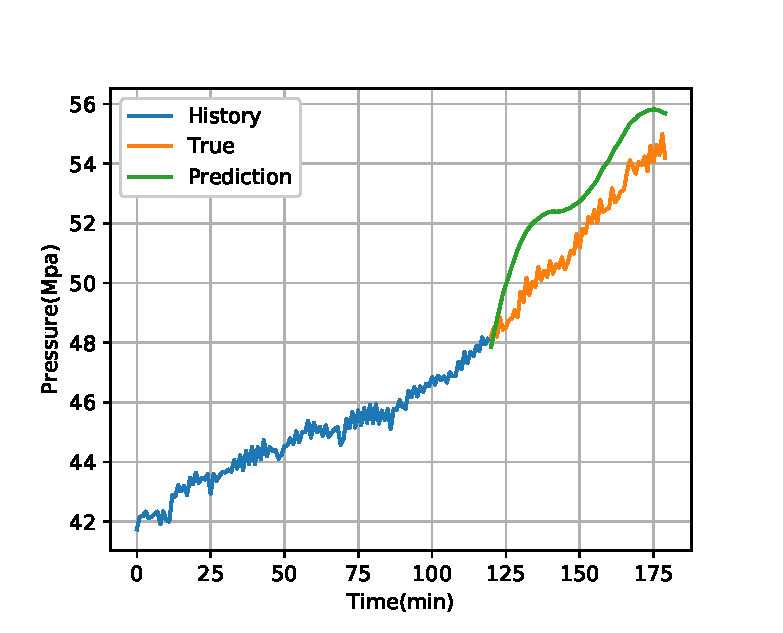
\includegraphics[width=\linewidth,trim=12 0 0 20,clip]{figures/chapter3/predict_cmp/Pressure_MLP_nonsta_rk4_60.eps}
% \hspace{-18pt}

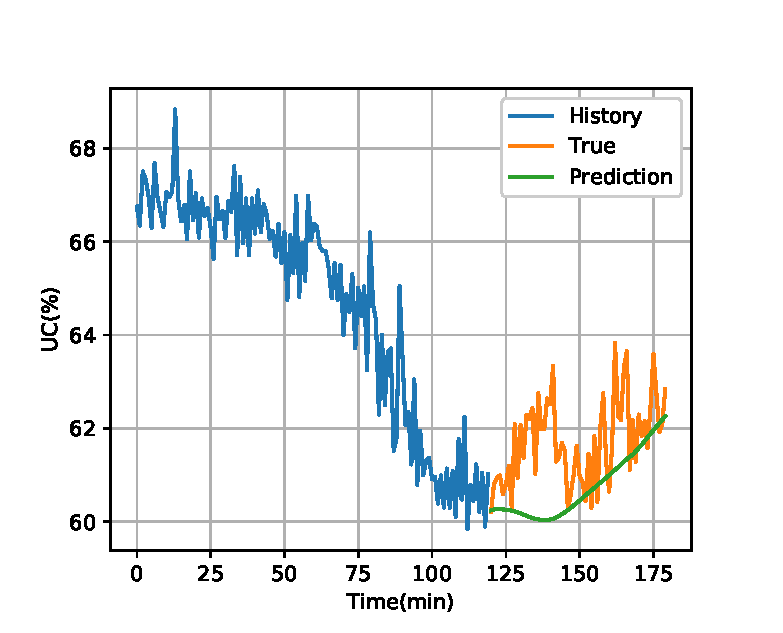
\includegraphics[width=\linewidth,trim=12 0 0 20,clip]{figures/chapter3/predict_cmp/UC_MLP_nonsta_rk4_60.eps}
%\caption{fig1}
\end{minipage}
}%
\hspace{-22pt}
\subfigure[非稳定系统+Dopri5求解器]{
\begin{minipage}[t]{0.33\linewidth}
\centering
% \hspace{-22pt}
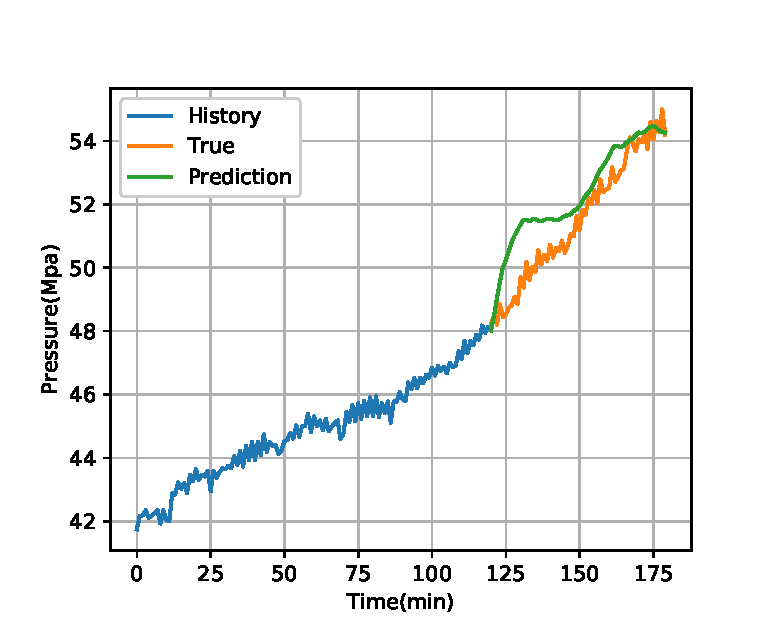
\includegraphics[width=\linewidth,trim=12 0 0 20,clip]{figures/chapter3/predict_cmp/Pressure_MLP_nonsta_dopri5_60.eps}
% \hspace{-18pt}

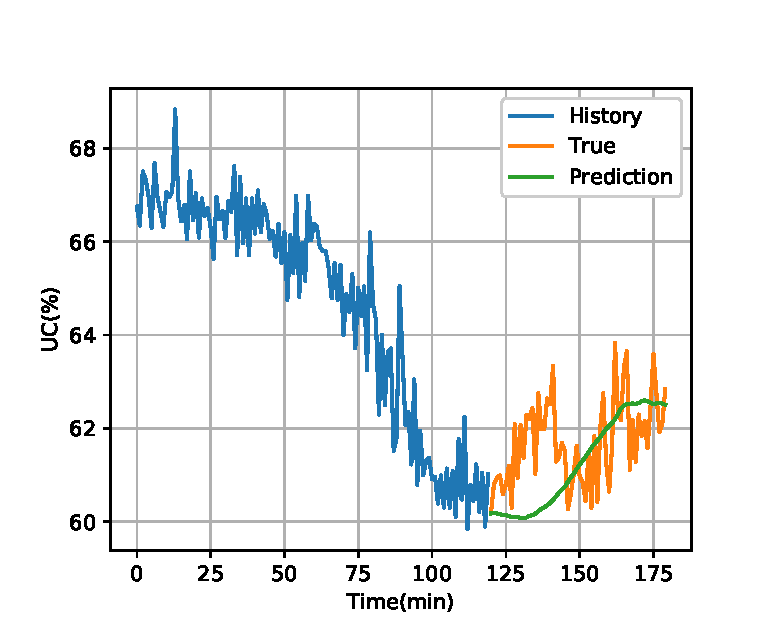
\includegraphics[width=\linewidth,trim=12 0 0 20,clip]{figures/chapter3/predict_cmp/UC_MLP_nonsta_dopri5_60.eps}
%\caption{fig1}
\end{minipage}
}%
\centering
\caption{不同系统及不同ODE求解器在$L=60$短期预测任务中的性能比较}
\label{fig:predict_cmp_60}
%\vspace*{-0.4cm}
\end{figure}

结果表明,非平稳模型在短期预测任务中的表现优于平稳模型。非平稳模型的估计序列比平稳模型的估计序列更接近实际系统输出。
非平稳系统的学习过程本质上相当于对隐状态进行差分,利用MLP网络学习平稳的系统一阶差分。
% The non-stationary system learns the evolution of internal hidden state which 
% The model with non-stationary system dynamic identifies the system smoothly because the structures constraint hidden state can only change in a continuous and slow form.
% TODO: 真的不想删,但是受篇幅限制暂时注释,以后有机会偷偷补上
此外,由于非稳定系统结构限制了隐状态只能以连续、缓慢的方式变化。因此模型可以平滑地预测系统的输出。该约束符合浓密机系统运行缓慢的特性,等价于缩小了模型参数的搜索空间,抑制了模型过拟合的情况。

图\ref{fig:predict_cmp_200}展示了长期预测任务($L=200$)中的模型预测结果。
% ($L=500$的类似结果可以在Table~\ref{tab:exp_all}中找到)。
\begin{figure}[t]
%\setlength{\abovecaptionskip}{-0.1cm} 
\centering
\subfigure[非稳定系统+RK4求解器]{
\begin{minipage}[t]{0.33\linewidth}
\centering
% \hspace{-22pt}
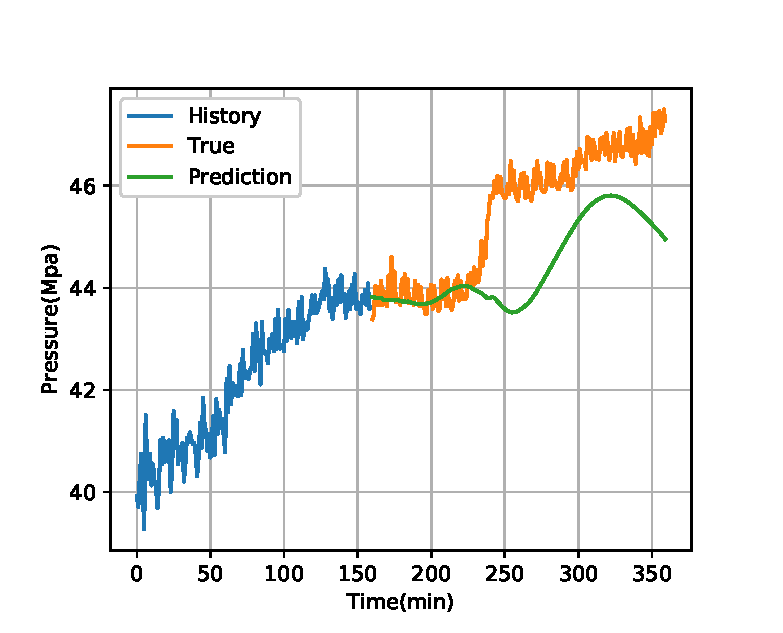
\includegraphics[width=\linewidth,trim=12 0 0 20,clip]{figures/chapter3/predict_cmp/Pressure_MLP_nonsta_rk4_200.eps}
% \hspace{-18pt}

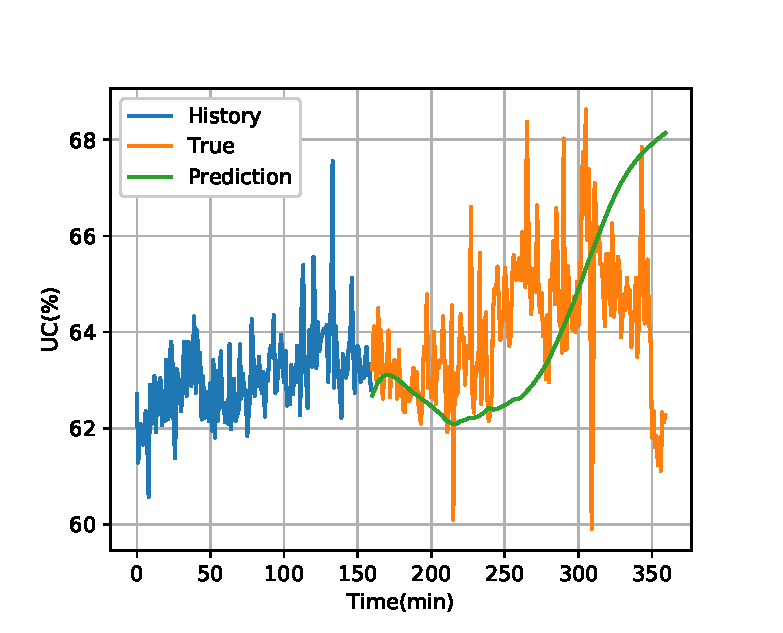
\includegraphics[width=\linewidth,trim=12 0 0 20,clip]{figures/chapter3/predict_cmp/UC_MLP_nonsta_rk4_200.eps}
%\caption{fig:subfig_200_nonsta_rk4}
\end{minipage}
\label{fig:subfig_200_nonsta_rk4}
}%
\hspace{-22pt}
\subfigure[稳定系统+Euler求解器]{
\begin{minipage}[t]{0.33\linewidth}
\centering
% \hspace{-22pt}
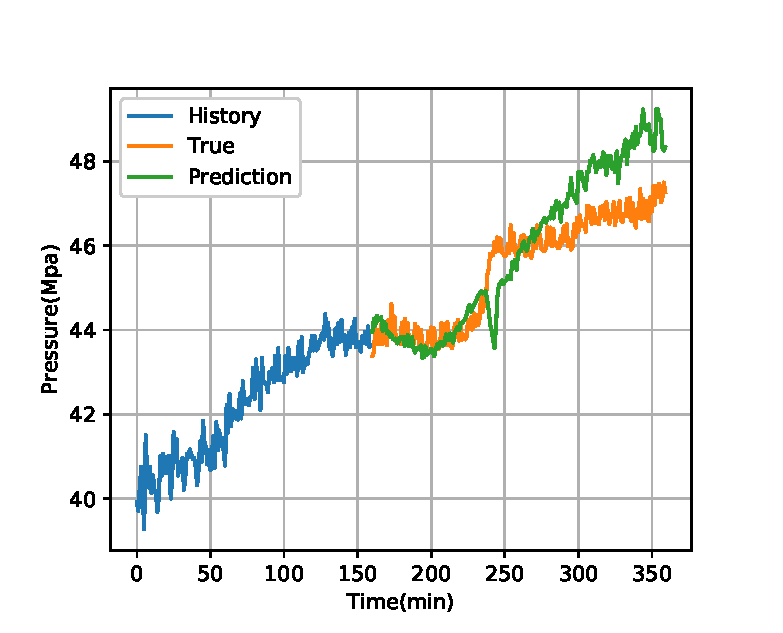
\includegraphics[width=\linewidth,trim=12 0 0 20,clip]{figures/chapter3/predict_cmp/Pressure_GRU_sta_euler_200.eps}
% \hspace{-18pt}

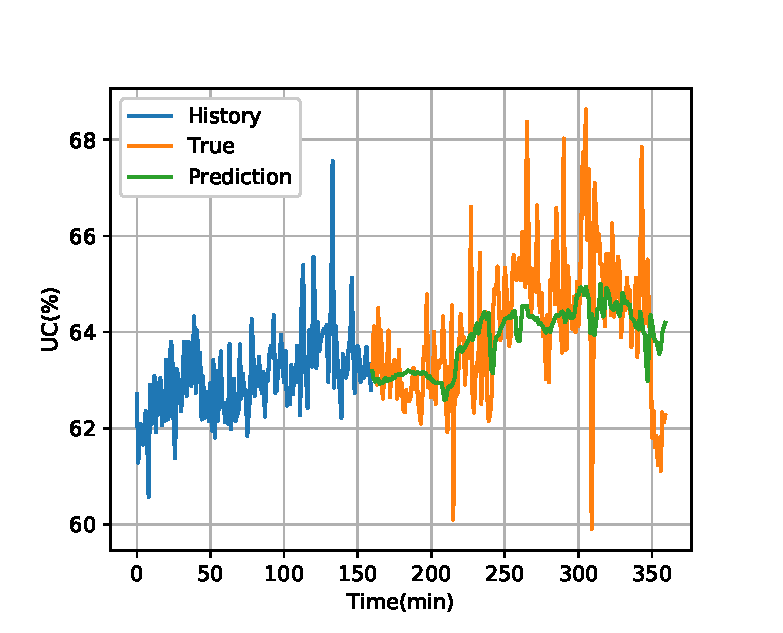
\includegraphics[width=\linewidth,trim=12 0 0 20,clip]{figures/chapter3/predict_cmp/UC_GRU_sta_euler_200.eps}
%\caption{fig:subfig_200_sta_euler}
\end{minipage}%
\label{fig:subfig_200_sta_euler}
}%
\hspace{-22pt}
\subfigure[稳定系统+RK4求解器]{
\begin{minipage}[t]{0.33\linewidth}
\centering
% \hspace{-22pt}
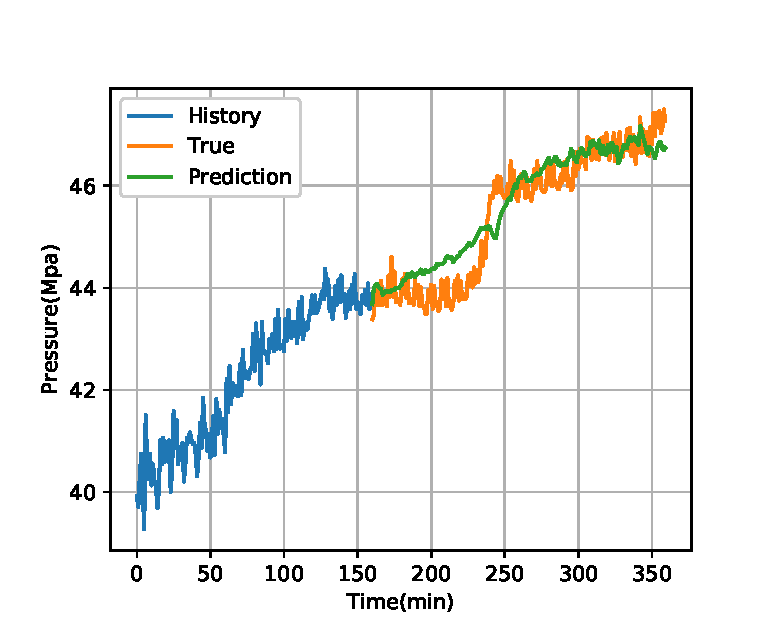
\includegraphics[width=\linewidth,trim=12 0 0 20,clip]{figures/chapter3/predict_cmp/Pressure_GRU_sta_rk4_200.eps}

% \hspace{-18pt}
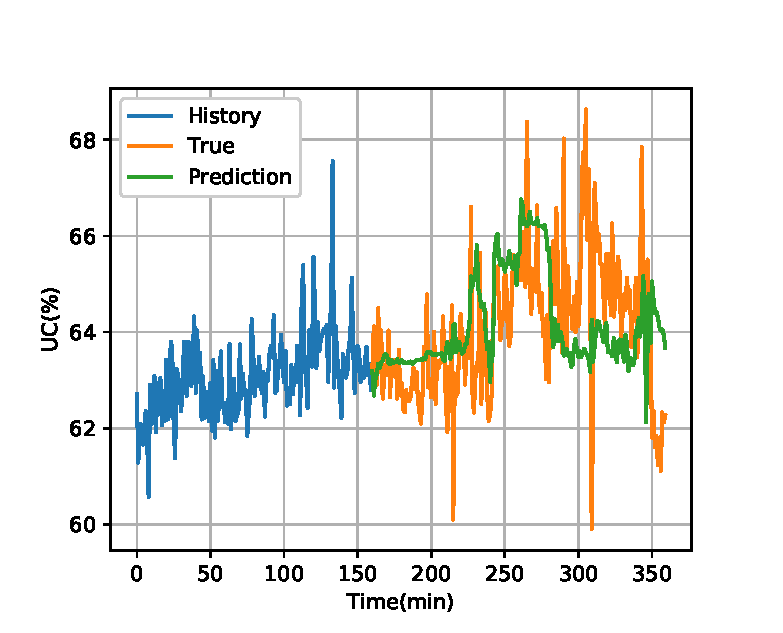
\includegraphics[width=\linewidth,trim=12 0 0 20,clip]{figures/chapter3/predict_cmp/UC_GRU_sta_rk4_200.eps}
%\caption{fig:subfig_200_sta_rk4}
\end{minipage}%
\label{fig:subfig_200_sta_rk4}
}%
% \subfigure[RNN-sta-Euler]{
% \begin{minipage}[t]{0.31\linewidth}
% \centering
% \includegraphics[width=1.1\linewidth]{figures/chapter3/predict_cmp/UC_RNN_sta_euler_200.eps}
% %\caption{fig2}
% \end{minipage}
% }%
\centering
\caption{$L=200$时,不同ODE求解器、系统动态的预测效果对比
} 
\label{fig:predict_cmp_200}
%\vspace*{-0.3cm}
\end{figure}
图中呈现的预测效果与表\ref{tab:exp_all}中的结果几乎一致。在长期预测任务中,非平稳模型的RRSE和MSE远远高于平稳模型,模型预测效果更差。
%It is meaningless to compare RRSE indices of results with different $L$, despite the RRSE in the experiments with $L=500$ is lower than $L=200$.
% When , we find that the model with stationary system performs lower prediction error than the non-stationary method.
% The illustrations of predicted results shown in Fig. \ref{fig:predict_cmp_200} and Fig. \ref{fig:predict_cmp_500} demonstrate that the non-stationary model only performs well in early period.
% The illustrations of predicted results shown in Fig. \ref{fig:predict_cmp_200} demonstrates that the non-stationary model only performs well in early period.
% We also illustrate the predicted results with $L=200$ in Fig. .
从图\ref{fig:predict_cmp_60}可以看出,非平稳模型在短期预测问题中获得较好的预测效果。
而在图\ref{fig:subfig_200_nonsta_rk4}中,非稳定系统在长期预测场景下的预测精度显著衰减,且预测偏离程度伴随着预测序列长度的增加而增加。
与之相对地,稳定系统的预测结果是稳定的,更接近于系统的真实输出,这证明了稳定系统模型在长期预测问题中具有更好的准确性。
% It is meaningless to compare RRSE indices of results with different $L$.
在由非稳定系统定义的导数模块中,其内部结构导致了隐状态在积分过程中是无约束的,状态的取值空间将逐渐扩张。
虽然模型在解码器网络中嵌入$\tanh$函数,能够将预测的系统输出限制在合理的范围内,但解码器模块无法学习有效的映射函数,实现从极大的隐状态空间到系统输出空间的准确映射。

同样地,图~\ref{Fig:predict_cmp_200}也证明了在长期预测问题中,高阶ODE求解器(如4阶Runge—Kutta)能够获得比低阶ODE求解器(如Euler)更好的预测效果。


% It notes that in the last part of simulation, the predicted system outputs deviate from the real sequences.
% The error is produced because thickening system is a partially observed system.
% Except for known external input or interference in $\b x(t)$, there exist plenty of invisible disturbances which affect the system extremely.
% The negative effects from unknown disturbances make the errors accumulated continuously over a long time period.
% In the long-term prediction task with $L=500$, the stationary model predicts the system outputs well in the former 300 minutes.




% TODO: 这部分也暂时注释,日后有机会再补上
%%%%%%%%%
% seek help: 自回归模型的缺点也是很明显的,每一轮循环的推理必须要在上一轮计算完成之后才能开始,ODE-net也不例外
% The disadvantage of autogressive model is also obvious that, each round of recurrent inference has to done after the last round finished, and ode-net is no exception.
% One disadvantage for autoregressive model is the recurrent inference must follow by rounds, so does ODE-net.
%%%%%%%%%

% 结果证实了基本rnn由于忽略了增稠系统的连续时间特性而不能很好地学习系统动力学方程的猜测。

从实验结果可以看出,采用自适应求解器的连续时间ODE-Net的预测表现优于其他欧拉近似法和龙格库塔近似法。
说明微分方程求解的精度会严重影响模型预测的精度。

虽然本文所提出的连续时间ODE-Net模型在预测精度上表现良好,但与其他模型相比,推理速度较慢。
表\ref{tab:exp_all}的最后一列表示预测序列长为$L$时,模型的平均消耗时间。
因为在ODE-net的训练和推理中,其前向传播和反向传播过程都需要大量地计算隐状态导数。
因此在预测系统动态变化时,其时间消耗远高于离散时间模型。
一些前沿研究\cite{J2020,poli2020,kelly2020}聚焦于优化ODE-net的训练或推理速度。
这些方法为提高本文模型的预测效率提供了有借鉴意义的指导。


本节额外进行了数组实验,以评估在不同预测长度$L$下,稳定系统和非稳定系统预测的底流浓度误差(MSE)变化。
图~\ref{fig:length_cmp}展示了五次重复实验中,底流浓度的预测误差波动情况($ log_{10}{\text{MSE}} \pm 2\sigma$)。虽然在长期预测任务中稳定系统优于非稳定系统,但非稳定系统在短期预测任务中的表现优于稳定系统(如$L<100$)。
大约当$L$超过$120$时,非稳定系统的误差随预测长度的增加而显著增加。
\begin{figure}[htpb]
%\setlength{\abovecaptionskip}{-0.1cm} 
    \centering
    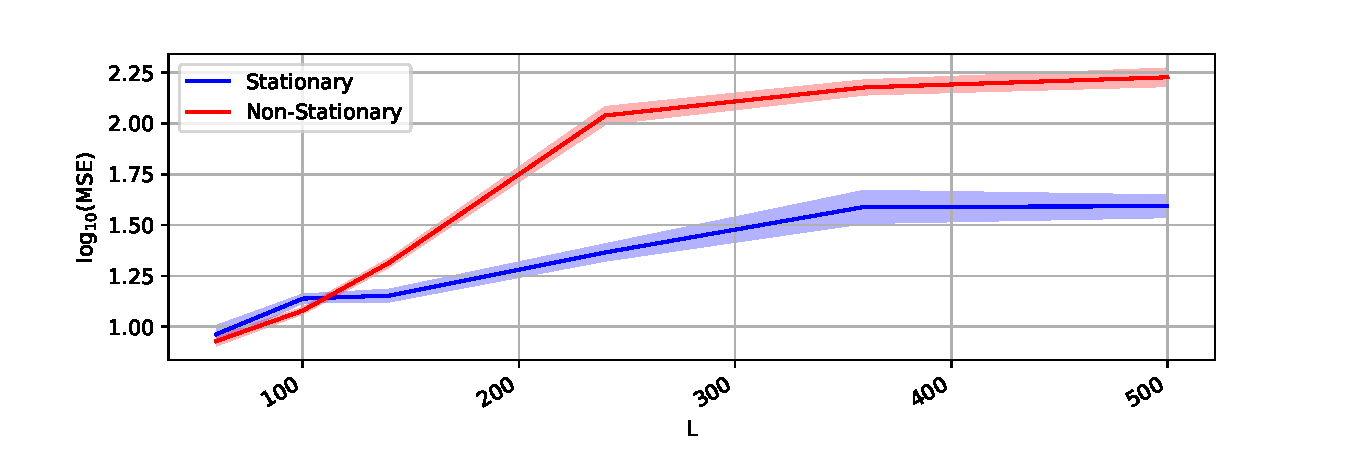
\includegraphics[width=\linewidth,trim=50 0 50 10, clip]{figures/chapter3/length_cmp.pdf}
    \caption{
    % The predicted length $L$ affects average $\log_{10}{MSE} \pm 2\sigma$ range of predicted underflow concentration for both stationary and non-stationary system.
    不同预测长度下稳定系统和非稳定系统的预测精度变化
    }
    \label{fig:length_cmp}
%\vspace*{-0.4cm}
\end{figure}

\subsection{探究序列插值阶数的对预测精度的影响}
本小节将进行消融实验,以探究对离散输入序列进行插值的方法是否对预测精度产生影响。
我们测试了四种不同阶数的样条插值方法,并比较了模型在测试集上的预测精度。
% The recurrent cell in experiment is RNN and the schema for solving ODE is RK4 uniformly.
表~\ref{tab:interolopation_cmp}的结果表明,模型中采用高阶插值的精度将稍优于低阶插值。
\begin{table}[h]
\centering
%\setlength{\abovecaptionskip}{-0.1cm} 
\caption{不同插值方法对预测精度的影响}
\renewcommand{\arraystretch}{1.5}
\label{tab:interolopation_cmp}
\begin{tabular}{c|cc|cc|cc}
\toprule
 \multirow{2}{*}{模型}         & \multicolumn{2}{c|}{\begin{tabular}[c]{@{}c@{}}$L=60$ \\ (120 minutes)\end{tabular}}                 & \multicolumn{2}{c|}{\begin{tabular}[c]{@{}c@{}}$L=200$ \\ (400 minutes)\end{tabular}}                  & \multicolumn{2}{c}{\begin{tabular}[c]{@{}c@{}}$L=500$ \\ (1000 minutes)\end{tabular}}                 \\
    & RRSE                 & MSE                  & RRSE                 & MSE                   & RRSE                 & MSE                   \\ \hline
三次样条插值     &  \uline{\textbf{3.083}} & \uline{ \textbf{8.565}} & \uline{ \textbf{3.581}} & 32.90                & 1.615                & \uline{\textbf{ 34.88}} \\
二次样条插值 & 3.097                & 8.993                & 3.593                &\uline{ \textbf{32.585}} &\uline{ \textbf{1.613}} & 36.741                \\
线性插值   & 3.098                & 8.999                & 3.763                & 33.530                & 1.627                & 37.778                \\
零阶样条插值      & 3.115                & 9.050                & 3.791                & 33.585                & 1.628                & 37.695                \\ \bottomrule
\end{tabular}
%\vspace*{-0.4cm}
\end{table}
这证明了本章所研究的膏体浓密机系统为复杂非线性受控系统,受控输入信息对于预测系统的输出是必不可少的。
高阶样条插值方法能够更充分地利用相邻位置离散输入信号的相关特征,相比于低阶插值方法,能够更精确地对空白区域进行插值填充。


\subsubsection{序列编码器的有效性验证及系统时延探究}
最后,本节探究了引入序列编码器对于解决含时延系统预测问题的有效性。
具体地,我们研究了序列编码器的有无以及不同的编码长度$N$对模型预测精度的影响。
特别地,当$N$设置为1时,将顺序编码器替换为具有单一隐藏层的神经网络,该神经网络将单步系统输出$\b y(k-1)$及输入$\b x(k-1)$编码为ODE系统的初始隐状态$\b h(t_0)$。
当$N$设置为0时,初始状态$\b h(t_0)$为可学习的初始隐状态\cite{Demeester2020SystemIW}或零向量,与历史系统轨迹不相关。

在不同的预测序列长度$L=60$、$200$和$500$的三个实验中,我们测试了不同的$N$对预测精度的影响。
在$L=60$的实验中,导数模块被设置为一个非平稳系统。
当$L=200$和$500$时,导数模块定义为带有GRU单元的稳定系统。
所有实验中,求解ODE方程采用四阶龙格-库塔求解器。

实验结果如表\ref{tab:seq2seq_cmp}所示,相比于令$N=0$,完全忽略系统历史输出,引入序列编码器并从历史运行轨迹中提取特征能够获得更好的预测精度。

\begin{table}[t]
\caption{不同初始隐状态 $\b h(t_0)$生成方法对于预测精度的影响}
\label{tab:seq2seq_cmp}
\centering
\renewcommand{\arraystretch}{1.5}
\begin{tabular}{|c|cc|cc|cc|}
\hline
\multirow{2}{*}{$N$}                                                & \multicolumn{2}{c|}{\begin{tabular}[c]{@{}c@{}}$L=60$ \\ (120 minutes)\end{tabular}}                 & \multicolumn{2}{c|}{\begin{tabular}[c]{@{}c@{}}$L=200$ \\ (400 minutes)\end{tabular}}                  & \multicolumn{2}{c|}{\begin{tabular}[c]{@{}c@{}}$L=500$ \\ (1000 minutes)\end{tabular}}                \\
\cline{2-7}
                                                                                     & RRSE                & MSE                 & RRSE                & MSE                  & RRSE                & MSE                  \\ \hline
160                                                                               & 3.11                & 9.08                &  \uline{\textbf{3.56}} & 34.13                & 1.61                & 35.88                \\
80                                                                                &  \uline{\textbf{3.10}} &  \uline{\textbf{8.97}} & 3.58                &  \uline{\textbf{32.92}} &  \uline{\textbf{1.61}} &  \uline{\textbf{34.88}} \\
40                                                                                & 3.19                & 8.99                & 3.65                & 36.07                & 1.71                & 41.26                \\ \hline
1                                                                                 & 4.06                & 10.71               & 4.97                & 51.09                & 1.77                & 63.56                \\ \hline
$N=0$,$\b h(t_0)$作为学习参数                  & 5.26                & 20.68               & 4.84                & 58.68                & 1.77                & 63.91                \\ \hline
$N=0$,令  $\b h(t_0)=\b 0$                                                                   & 5.26                & 23.11               & 5.84                & 64.49                & 1.77                & 63.53                \\ \hline
\end{tabular}
\end{table}
其直观解释为,待预测的系统输出序列与历史系统轨迹具有很强的统计相关性,从后者提取的特征对于序列预测有很重要的意义。
根据实验发现,被编码序列的最优长度约为$N=80$,这与浓密机系统存在2至 3小时时延的先验经验几乎一致。

直观上看,短期预测任务比长期预测任务更能从历史系统轨迹中获益。随着被预测序列长度的增加,引入序列编码器带来的优势也随之降低。在$L=500$的任务中,使用顺序编码器得到的预测精度约等于将$\b h(t_0)$作为学习参数的初始状态编码方案。
\section{本章小结}
\label{sec:conc}
本章针对高时延工业多输入输出系统预测问题,
提出了一种基于ODE-net的连续时间网络模型,该模型由顺序编码器、状态解码器和导数模块三部分组成,模型的内部计算过程包括历史序列编码、离散输入序列插值以及常微分方程求解三部分,模型能够从连续时间域角度拟合复杂系统的动态过程。
在膏体浓密机系统运行数据集上,我们进行了大量实验对所提出模型的各个部分进行研究,包括平稳系统和非平稳系统的选择以及不同ODE求解器的设定。
结果表明,非平稳系统在短期预测任务中的表现优于平稳系统。
但是,非平稳模型由于存在累加计算,会造成隐状态的波动范围过大,进而导致长期预测性能较差。
该结果表明非平稳系统模型更适用于短期预测场景,如基于模型的反馈控制器(如MPC控制器)中作为预测模型辅助控制器输出。
而平稳系统通过修改了导数模块结构,避免了隐状态漂移问题,因此在长期预测中表现较好。
因此,当需要具有较强稳定性、鲁棒性的系统识别模型进行系统长期预测时(如系统仿真或控制器测试),具有平稳系统的模型是更好的选择。
同时,通过消融实验表明模型中引入序列编码器和并行三次样条插值对于模型精度的提升起到了至关重要的作用。
在工业数据分析领域,面向不均匀采样数据的分析与预测是极其常见的。虽然本文所用数据集的采样间隔是均匀的,由于本文所述模型是基于ODE-net进行构建的,具有连续时间域的系统学习及表示能力,因此该方法可以很自然地处理不均匀数据。
该问题值得在今后的工作中被进一步的验证。
另外将本文方法扩展为概率模型和时变模型,以辅助确定复杂系统中的未知噪音和不确定性,也是未来极具价值的研究方向。


% %第四章


\chapter{基于自跳跃常微分方程网络的连续时间跳变系统建模}
周期性跳变系统在现实生活中随处可见,其运行过程具有周期循环性。每个周期内,各阶段之间按特定顺序进行切换。系统在不同阶段会呈现明显不同的动态特性。
例如,洗衣机启动后将按程序设定,周期性地在进水,洗涤,排水,甩干各个阶段之间循环运行,直至最后关机。
冰箱和空调在工作期间会在运行(压缩机开启)和待机(压缩机关闭)两种状态之间不断进行切换。
在一些自然界中其他的物理过程,也存在类似的系统,例如建筑物内的空调制冷系统、交通流量和季节变化等。
% 在使用自回归模型对具有周期多阶段特性的系统进行预测时,我们希望模型能够自动地在特定时刻进行状态转移。
例如,在对城市交通流量或某产品销量进行预测时,流量或销量通常伴随着特定的日期和季节变化而改变,并且其周期长度相对稳定,模型能够较容易地识别各预测时刻被预测对象所处的阶段。
相反,对于一些复杂工业系统,其周期长度可能受到系统内部和外部多个变量的影响。
例如系统的外部输入、当前内部状态、环境条件等。
利用历史运行数据识别以及建模此类跳变系统对于理解和优化系统运行过程是极其重要的。
% 对于此类带有多阶段特性的复杂工业系统,想要采用单一模型学习具有不同阶段特性的动态并且实现精确的系统预测与仿真是极其困难的。
然而,在面向跳变系统进行建模时面临两大技术难题。首先,
跳变系统通常有多个阶段,每个阶段呈现不同的非线性特性。各个阶段的持续时间可能同时受到内部因素和外部因素的影响\cite{WANG2022111790}。目前,面向跳变系统参数估计方法\cite{balenzuela2022parameter}通常依赖于对系统结构以及持续时间分布的先验认知,这需要大量的领域专家知识作为支撑。
另外,对于带有多输出项的工业系统,其输出过程可能由
多个不同的物理特性共同影响。这会导致多输出项中同时存在稳定和非稳定过程\cite{nason2006stationary}。
据我们所知,对于现有的未经过特定设计的现存模型,难以解决此类带有混合时序特性的系统学习任务。

为了实现上述目标,模型需要解决两个问题。
首先,模型需要根据系统的外部输入以及系统状态,识别在当前时刻系统所处的阶段。
另外,模型需要能够准确地识别系统在各阶段内的独立动态特性。
针对上述挑战和问题,本章提出了一种新颖的自跳跃常微分方程网络(Autonomous jump ordinary differential equation net, AJ-ODEnet)以学习连续时间周期跳变系统。
该模型是一种新颖的连续时间深度学习模型,能够从非均匀采样的系统历史轨迹进行学习。
% 该框架主要用于建模具有周期性多阶段转换的多输入输出系统,利用数据驱动的方式从系统输出序列中学习系统不同阶段的动态特性。
训练完成后,对于给定的系统外部输入模型能够实现实时在线预测。
为了学习系统在不同阶段的动态特性,模型包含多个层次常微分方程网络(Hierarchical ODENets ,H-ODENets)
层次常微分网络是一种双层扩展的常微分方程网络,能够同时学习系统的稳定过程和非稳定过程。
为了学习阶段转换,本章对原始训练数据进行了阶段类别标注,并在模型中引入阶段转换预测器学习每个阶段的持续时间。
阶段转换预测器由多个持续时间预测器构成,在开环预测和仿真中,阶段转换预测器能够作为H-ODENets的调节器,在每个时间点指派合适的H-ODENet进行系统输出的预测,并预估当前所处阶段的持续时间,进而实现自发的阶段转移。

% 为了使模型能够从数据中自动地学习各阶段内的系统动态特性,针对待预测系统输出同时存在非稳定过程和稳定过程的问题,引入分层常微分方程网络。
% (hierarchical ODEnets, H-ODEnets)实现对系统多维输出的混合学习。

% 因此,在本章提出的AJ-ODEnets模型中,参考了有限状态机的基本思想,构建了可学习的阶段转换模块。
同时为了给定求解AJ-ODEnet的状态初值,本章遵循编码器解码器(Encoder-Decoder)范式,构建了两个AJ-ODEnet分别用于历史数据的编码以及在给定的系统输入序列下以开环的方式预测系统的未来输出。
除此之外,本章引入样条插值算法,以连续化离散的输入序列并作为AJ-ODEnet模型的输入。
最后,本章将所属模型及框架应用于某一具有典型周期多阶段特性的工业制冷系统的预测与仿真问题中。
通过给定系统的多变量运行数据,包括热负载以及环境温度,模型能够仿真系统的运行过程并准确地预测系统能耗(能耗预测误差小于5\%)。
进一步地,通过模型的仿真功能能够优化系统的制冷温度设定参数,通过仿真实验表明利用优化之后的温度设定值能够显著改善能源利用效率并且节省超过25\%的制冷能耗。
% 本章所述模型能够有效地模拟制冷系统的运行,预测其功率消耗以及服务器进气口温度。

% Addressing the challenges and problems mentioned above, we propose AJ-ODEnets, a novel framework for modeling and identifying the non-linear dynamics at different stages in periodic operational systems. The framework is specifically capable of capturing physical dynamics thanks to the implementation of ODEnet, a neural network based on ODE. The framework is expected to learn the multivariate inputs-ouputs system in a data-driven way, by feeding several sequences of sensory data as training data. Once trained, the model is able to realize real time predictions according to the multivariate inputs. Modeling multi-stage periodic systems requires two principal realizations, one for the stages prediction, one for dynamical characteristics identifications of different stages. 





% With this purpose, in the design of AJ-ODEnets, a selective structure is considered.
% In terms of learning dynamical characteristics at different stages,
% the framework contains several hierarchical ODEnets (H-ODEnets), and the number depends on the observed system stages. H-ODEnets can be seen as an extension of ODEnet, which can deal with both stationary and non-stationary sequences. 
% In terms of learning the system transitions during operation, a stage transition predictor is included in the AJ-ODEnet module, which can infer the transfer actions from a sequence of observation data, specifically, when and how to change to other tendency during system operation. In order to train the stage transition predictor, the observation data has been labeled previously in a conditional data range, based on prior knowledge of the system operational specifications. During predictive range, the stage transition predictor serves as the governor to appoint to the suitable H-ODEnet, so as to let the system run across different working stages periodically. Adaptive smoothing algorithm is introduced to impute missing data as well, it can handle nonlinear and irregularly sampling data, which is practical in dealing with sensory data from IoT systems. The AJ-ODEnets framework has been further implemented in a running data center with contained structure, to simulate the cooling system operations. 

本章研究主要包含三方面贡献,概括如下:
\begin{itemize}
    % \item 首先,本章将原始的ODE-net模型扩展到H-ODEnet模型,能够学习同时带有稳定和非稳定时间序列输出的动态过程。
    \item 为了辨识连续时间跳变系统,本章提出了一种新颖的深度学习模型——自跳跃常微分方程网络模型。该模型能够实现
    (1)在一个集成化的网络中学习系统的多阶段动态,(2)在长序列开环预测中实现阶段自转移。
    % \item 其次,本章针对具有周期多阶段特性的动态系统,开创性地提出了AJ-ODEnets模型,该模型通过引入阶段转换预测器学习系统的周期性阶段转换以及采用多个H-ODEnets学习不同阶段内的系统动态特性。
    \item 为了学习同时包含稳定和非稳定项的多输出系统,本章结合每个输出项的统计特性,引入H-ODENet以改善两种输出项在长期预测中精度。
    \item 本章所述模型成功应用于某一工业制冷系统的预测与仿真问题中,该模型能够在给定热负载功率下,准确地预测制冷系统的功率消耗以及制冷气温度变化,依托于该仿真模型能够优化制冷系统的工作温度设定值,进而优化制冷系统的整体能耗约25\%。
    
\end{itemize}
% Two main contributions are devoted to this study, summarized as follows::
% \begin{itemize}
%     \item First, we extent the original vanilla ODE-net to the Hierarchical ODEnet (H-ODEnet), which is able to learn the stationary and non-stationary time series data simultaneously.
%     \item Second, we propose AJ-ODEnets framework, targeting at learning periodic multi-states systems in data-driven way. AJ-ODEnets disposes of several H-ODEnets to automatically learn dynamic characteristics at different states, along with a stage transition predictor to learn the transition actions during operation. 
% \end{itemize}

本章的结构组织如下:
本章\ref{sec:notations}节给出了变量符号定义以及描述了周期性多阶段系统预测问题的形式化描述。
本章\ref{sec:h-ode}节介绍了分层常微分方程网络的定义及结构,以及如何将其用于学习同时带有稳定和非稳定时间序列输出的动态过程。
本章\ref{sec:dfa-odenet}介绍了AJ-ODEnet框架,并详细阐述了连续时间域下的状态转移方程、关键模块结构和持续时间预测器的损失函数定义等内容。
本章\ref{sec:encoder_decoder}给出了基于AJ-ODEnet模型的编码器解码器框架及其训练方法。
本章\ref{sec:evalutaion}节介绍了将所述框架应用于模拟某实际工业制冷系统。模型能够根据制冷系统的热负载输入对其功耗以及出气口气体温度变化进行模拟预测,同时能够实现不同制冷启动温度配置下的功耗仿真与优化。
最后,\ref{sec:conclusion}节对本章工作做出了总结,并对AJ-ODENet模型的潜在应用以及未来的研究方向做出了讨论。


% The paper is organized as follows: related work on time series prediction for industrial systems, and for multi-state systems are summarized in Sec.~\ref{sec:review}. Then, preliminary in Sec.~\ref{sec:preliminary} describes the basic theory used in this study. After that, in Sec.~\ref{sec:methodology_dfaode}, the proposed framework AJ-ODEnet is detailed in terms of data processing, structure of key modules and training for loss functions. In practice, the proposed framework is applied to simulate several working variables of a cooling system in real data centers. Two use cases are included, one for real time estimation of the energy consumption based on system inputs and environmental condition, and the other takes advantage of the integrated prior knowledge, simulations are conducted to optimize the consumption by varying configurations. In the end, Sec.~\ref{sec:conclusion} concludes the entire work and discuss the potential future work.
\section{前置工作及问题形式化描述}
\label{sec:notations}
连续时间跳变系统(Continuous-time Jump System,CTJS)由多个连续时间子系统组成,其内部阶段转换由一个有限状态过程支配\cite{8709809}。
% As an important class of dynamical systems, CTJS arises in many applications, such as failure prediction\cite{9165930}, control applications\cite{pmlr-v120-jansch-porto20a}, and state estimation\cite{8709809}.
作为一种特殊的动态系统,CTJS系统广泛应用于各类应用中,如故障预测\cite{9165930}、系统控制\cite{pmlr-v120-jansch-porto20a},以及状态估计\cite{8709809}。
典型的连续时间跳变系统定义形式如下:
\begin{equation}
    \dot{\boldsymbol h}(t)=\mathcal{F}_\sigma(t)(\boldsymbol h(t), \boldsymbol x(t),
    \label{equ:ctjls}
\end{equation}
% where $\sigma(t)\in\{0,1\cdots N-1\}$ is a finite-state step process and $\boldsymbol{x}(t)$ is system inputs with the Lipschitz continuity.
% With different $\sigma(t)$, the non-linear system dynamics $\mathcal{F}_{\sigma(t)}$ are distinct.
% Compared to a general continuous-time markov jump system whose state $\sigma(t)$ is a markov process, this study assumes that the transition of $\sigma(t)$ is deterministic and circular.
% Specifically, in a continuous-time periodic jump non-linear system, the piece wise constant state $\sigma(t)$ jumps in a cycle order $\{0,1,\cdots,N-1,0 \cdots\}$.
% The sojourn time between jumps depends on the trigger thresholds according to prior knowledge about the system.
% To distinguish between the state in a system and the hidden state in a recurrent neural network, we name the system state $\sigma(t)$ as the \textbf{\textit{stage}} in this paper.
其中$\sigma(t)\in\{0,1\cdots N-1\}$为一有限状态集下的跳变状态,$\boldsymbol{x}(t)$为满足利普希茨连续的系统输入。
在一般的连续时间马尔科夫跳变系统中,系统状态$\sigma(t)$的变化遵循马尔科夫过程。相比之下,本章假设阶段变量$\sigma(t)$的转移是确定性地且循环的,并将此系统定义为连续时间周期跳变非线性系统中(Continuous-time periodic jump non-linear system),分段恒定的状态$\sigma(t)$在循环$\{0,1,\cdots,N-1,0 \cdots\}$中不断变化。
状态跳跃之间的停留时间取决于由系统先验属性决定的触发条件。
为了明确区分跳变系统中的状态变量$\sigma(t)$以及以及循环神经网络中的隐状态,本章将跳变系统状态$\sigma(t)$命名为阶段。
% 基于模型驱动的参数估计或系统辨识方法有时很难被应用于复杂的跳跃系统中,因为实际的动态行为很难被识别。为了从现有的输入输出数据中学习CTJS,以前的研究假设了系统的先验结构,并采用了EM算法(balenzuela2022parameter}、顺序蒙特卡洛(SMC)(6859280)和变异推理(opper2007variational)等方法来估计模型参数。

在本文中,标量和向量在形式上分别用小写字母和粗体小写字母表示,例如$y, \boldsymbol y$。假设输入输出数据由传感器观测得到,并带有时间戳$t_i\in \mathbb{R}$。
因此,从系统中采集的带有非均匀采样间隔的离散输入序列和输出序列可表示为:
$\boldsymbol X_{1:I},\boldsymbol Y_{1:I}= ((t_1,\boldsymbol x_1,\boldsymbol y_1),(t_2,\boldsymbol x_2, \boldsymbol y_2),\cdots,(t_I,\boldsymbol x_I,\boldsymbol y_I))$. 
%with each $t_i\in \mathbb{R}$ the timestamp of the system input and output, and $t_{0}<\cdots<t_{n}$.
% we define $\boldsymbol y_i$ as the $i$-th vectorial variable in a discrete sequence. 
相应的,定义$\boldsymbol x(t_i)=\boldsymbol x_i$ 以及 $\boldsymbol y(t_i)=\boldsymbol y_i$。
其连续时间过程可表示为$\boldsymbol x:\left[t_{1}, t_{I}\right] \rightarrow \mathbb{R}^{M}$ and $\boldsymbol y:\left[t_{1}, t_{I}\right] \rightarrow \mathbb{R}^{N}$.
为了便于后文描述,本章将$\boldsymbol y:\left[t_{1}, t_{I}\right]$简化为$\boldsymbol Y_{t_1:t_I}$

本章所关注的问题为根据系统的历史数据信息和以及系统的未来序列输入,预测系统的未来输出。具体地本章对于给定数据的时间范围$[t_1:t_{I+L}]$分为两部分,分别作为条件范围$[t_1:t_{I}]$ 和预测范围$[t_{I}:t_{I+L}]$。
%Given $\{{\boldsymbol{X}}_{t_{1}:t_{I+L}}, {\boldsymbol {Y}}_{t_{1}:t_{I+O}}\}$, the system inputs and system outputs in time range $[t_1:t_{I+O}]$,
% , where ${\boldsymbol y}^i_{1:I+O}=[{\boldsymbol y}^i(t_1),\boldsymbol y^i(t_2),\dots,{\boldsymbol y}^i(t_{I+O})]$ and ${\boldsymbol y}^i(t_j)$ is the $j-th$ value in $i-th$ system outputs series collected at time $t_j$ . 
模型通过给定条件范围$[t_1, t_I]$下的系统输入和系统输出生成初始状态,然后对预测范围$[t_{I}, t_{I+L}]$下的系统输出进行预测,如式~\ref{equa:problematique}所示:

\begin{equation}
\label{equa:problematique}
    \hat{\boldsymbol Y}_{t_{I}:t_{I+L}} = f(\boldsymbol Y_{t_{1}:t_{I}}, \boldsymbol X_{t_{1}:t_{I+L}};\boldsymbol \zeta) 
\end{equation}
公式中$\hat{\boldsymbol Y}_{t_{I}:t_{I+L}}$表示在预测范围内估计的输出。 
$\boldsymbol Y_{t_{1}:t_{I}}$表示在条件范围内系统的历史输出。
$\boldsymbol X_{t_{1}:t_{I+L}}$表示完整时间范围内的系统输入,包括历史部分和预测序列部分。该系统输入在时间序列预测领域经常被称为协变量\cite{Wu2020}。
$\boldsymbol \zeta$表示利用数据集训练的模型可学习参数。
本章的目标为通过优化$\boldsymbol \zeta$以最小化$||\hat{\boldsymbol Y}_{t_{I}:t_{I+L}}-\boldsymbol {Y}_{t_{I}:t_{I+L}}||^2$
% Where $\hat{\boldsymbol Y}_{t_{I}:t_{I+L}}$ is the estimated outputs in predictive range. $\boldsymbol Y_{t_{1}:t_{I}}$ represents the historical system outputs in conditional range.
% $\boldsymbol X_{t_{1}:t_{I+L}}$ is the system inputs of whole range that involve both historical and predictive parts.
% $\boldsymbol \zeta$ is the learnable parameters of model trained jointly from all available datasets. \\

% The formulation in Eq.~\eqref{equa:problematique} is similar to the time-series forecasting problem, which focuses on extracting temporal information and predicting the future outputs given historical observed targets and covariates \cite{Lim2021}.
% \eqref{equa:problematique}所示的形式化描述类似于时间序列预测问题。
% Time series forecasting methods are employed for extracting temporal information and predicting the future outputs given historical observed targets and covariates \cite{Lim2021}.
% However, the research scope of this paper is more related to the field of system modeling/identification , which focuses on modeling the dynamics of the system.
% The historical system observations herein are mainly utilized to provide an accurate initial state.
% With an inferred initial state, the model can predict the system outputs in open loop, based on the given system inputs in a predictive range. 
% The length of the predictive range is determined according to the length of the simulation we want to make.
% Taking the studied cooling system simulation as an example, we can theoretically feed arbitrary long heat loads as inputs and the model will simulate the corresponding temperature variation in that predictive range.
以制冷系统为例,可以将任意长度的热负载序列数据作为模型输入,模型能够仿真预测区间下的温度变化。
值得注意的是,本章仍关注开环预测问题,模型预测过程中无法收到来自系统输出的反馈。对于存在随机性及非确定性的系统,长期开环仿真是难以实现精准预测的。
因此,在训练阶段,预测范围长度与条件范围长度是一致的,为800s。
在实验一中,预测范围的长度为30分钟,本章考虑到由于误差累积导致的相位偏差,因此没有采用点对点式的评估指标,而是采用预测累积能耗的估计误差对模型可靠性进行评估。

% However, when there is no feedback from system outputs, the long-term open-loop simulations are unreliable for a stochastic or uncertain system.
% In Section \ref{sec:case-study1}, although the length of the predictive range is altered to 30 minutes, 
% we considered the accumulated estimated error of phases positions and give up the point-to-point evaluation and seek other evaluation indicators


\section{基于层次ODE-Net模型的复杂系统稳定及非稳定输出混合预测}
\label{sec:h-ode}
大部分工业系统的输出是多维度的,不同维度输出的时序统计特性存在一定差异,某些输出量为均值方差恒定的稳定过程,某些输出为均值方差不断变化的非稳定过程。
对于同时含有稳定和非稳定输出的混合过程进行建模学习具有一定难度,当前主流的基于深度学习的序列预测领域并未针对该类系统开展研究。
针对该问题,本章提出了分层常微分方程网络(Hierarchical ODENet, H-ODEnet),用于建模同时包含稳定过程和非稳定过程的系统。

具体地,H-ODEnet将三个ODEnet集成为双层结构(L-1和L-2)。
% Modeling hybrid processes with both stationarity and non-stationarity properties is another challenge for industrial systems, as existing methods normally target one situation. With this in mind, Hierarchical ODE-net (H-ODE) is proposed to model a system containing non-stationary and stationary processes simultaneously. In 图.~\ref{fig:AJ_ODEs}, there are $N$ number of H-ODEnet embedded in the AJ-ODEnet module, and only one will active at specific time point $t$, based on state variable $\sigma(t)$. In detail, H-ODE hierarchically integrates a two-level structure (L-1 and L-2) with three ODEnets.
% to deal with the mixed situations mentioned above.
%The learned continuous-time predictive model is named Hierarchical ODE-net which hierarchically integrates a two-level ODE-net.
图~\ref{fig:H_ode}展示了H-ODE中三个ODE-net之间的连接方式。
\begin{figure}
    \centering
    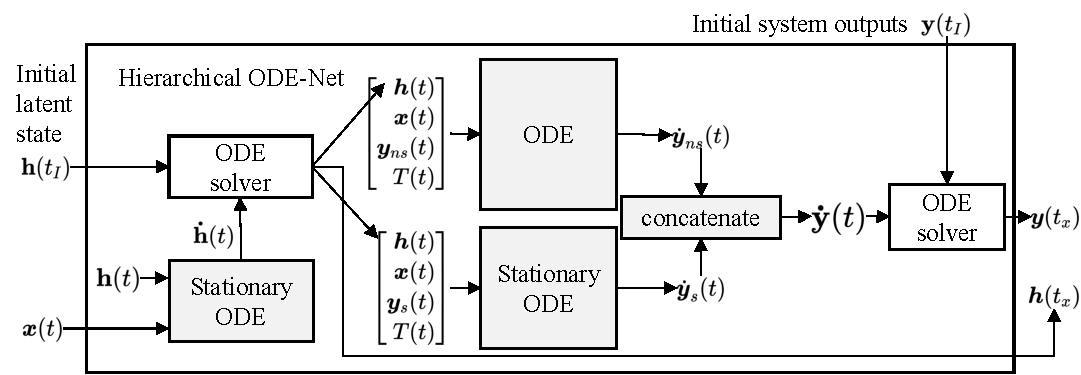
\includegraphics[width=\linewidth]{figures/chapter4/Hode.pdf}
    \caption{H-ODEnet结构图示}
    %\caption{An H-ODEnets consists of three ODE-net. The high-level ODE-net estimates the derivative of latent state according to external inputs. By integrating the ODE equation with high-level ODE-net, the solved $\boldsymbol h(t)$, accompanied with external inputs $\boldsymbol x(t)$ and duration time of current stage $T(t)$, is fed into two low-level ODE-nets to estimate the derivatives of system outputs. The predictions of system outputs at arbitrary time points $t_x$ can be solved by integrating the low-level ODE-nets.}
    \label{fig:H_ode}
\end{figure}
在L-1层中,包含一个ODEnet,用于根据外部输入对隐状态的导数进行建模。利用实时求解出的$\boldsymbol h(t)$、外部输入$\boldsymbol x(t)$和当前阶段持续时间$T(t)$,对由L-1中的ODE-net定义的常微分方程进行积分。解出的$\boldsymbol h(t)$作为L-2中两个ODE-net的输入,并分别用于求解稳定系统输出项和非稳定系统输出项的导数,表示为$\boldsymbol y(t)=[\boldsymbol y_s(t), \boldsymbol y_{ns}(t)]$。
最终,可以解出任一时间点$t_x$下的预测结果。

% 图.~\ref{fig:H_ode} illustrates the connections between three ODE-nets within H-ODE. The L-1 contains one ODEnet to model the derivative of
% %The high level part of H-ODEnet is an ODE-net that 
% latent state according to external inputs. By integrating the ODE equation with ODE-net of L-1, the solved $\boldsymbol h(t)$, combined with external inputs $\boldsymbol x(t)$ and duration of current stage $T(t)$, are fed into L-2 ODE-nets to model the derivatives of stationary and
% %the stationary system outputs and 
% non-stationary system outputs, denoted as $\boldsymbol y(t)=[\boldsymbol y_s(t), \boldsymbol y_{ns}(t)]$ respectively. The predictions at arbitrary time points $t_x$ are solved in the end. 
%and the low-level part consists of 
%and only one particular H-ODEnet corresponding to $s(t)$ may be utilized to make prediction at time point $t$.
%To utilize one model to predict a system involving the non-stationary and stationary process simultaneously, we propose a hierarchical ODE-net whose three ODE-nets predict the derivative of latent state, the derivative of stationary system outputs and the derivative of non-stationary system outputs respectively.

其中,L-1中的ODEnet为稳定结构,由门控循环单元(GRU)网络实现\cite{Demeester2019}:

% The ODEnet in L-1
% %for modeling latent state 
% is stationary and implemented by stationary Gate Recurrent Unit (GRU) network\cite{Demeester2019}:
\begin{equation}
    \label{equ:dh}
    \frac{d \boldsymbol{h}(t)}{\tau} = \frac{1}{\mu(t)}*\left[\text{GRU}(\boldsymbol{x}(t), \boldsymbol{h}(t),\text{sigmoid}(T(t)), \theta^\mathcal{H}_{\sigma(t)}) - \boldsymbol{h}(t)\right]
\end{equation}
其中$\mu(t)$表示原始数据集的平均采样间隔均值。
稳定的GRU网络将预测的隐状态变量$\boldsymbol{h}(t)$的变化表示为稳定过程,并将其上下界限制在$(-1,1)$范围内。


% where $\mu(t)$ denotes the mean of sampling intervals in entire dataset.
% Stationary GRU network treats the predicted latent state $\boldsymbol{h}(t)$ as a stationary process and constrains the outputs within range $(-1,1)$. 
% In comparison to stationary model which produces stabilized latent state, incremental models(non-stationary model) suffers from potentially linearly growing state, which is ill-suited for modeling long-term stationary time series~\cite{Demeester2019}.

% unit root problem and bring in long-term prediction.
% potentially linearly growing state is ill-suited for modeling stationary time series
%The low-level ODE-nets

L-2中的两个ODEnet被分别设计用于建模稳定和非稳定的系统输出。
其中用于建模非稳定输出的网络采用非稳定增量形式预测输出$y_{ns}(t)$ :

% The two ODEnets in L-2 are designed to %is utilized to model the instant derivatives for system outputs in using two ODEnets 
% cover both stationary and non-stationary cases.
% % In this study, consumed power of cooling system $y_1(t)$ and cooling capacity $y_2(t)$ are categorized as stationary outputs, $\boldsymbol{y}_{s}(t)=[y_1(t), y_2(t)]^T$.
% % The inlet temperature of cooling system $y_3(t)$ is categorized as non-stationary outputs, $\boldsymbol{y}_{ns}(t)=[y_3(t)]^T$. 
% The one for $y_{ns}(t)$ is employed by implementing non-stationary incremental neural network:
% %One of low-level ODE-nets, implemented by an non-stationary incremental neural network, is employed to model non-stationary outputs:
\begin{equation}
    \label{equ:dyns}
    \frac{d \boldsymbol{y}_{ns}(t)}{\tau} = \text{NN}(\boldsymbol{x}(t), \boldsymbol{h}(t), \text{sigmoid}(T(t)), \theta^{\mathcal{Y}^{ns}}_{\sigma(t)})
\end{equation}

另一个ODEnet类似于L-1中的ODEnet,由一个稳定的GRU模型构建,用于预测系统的稳定输出$y_s$:
% Another ODEnet for $y_s$ is similar with the one in L-1, which is implemented by a stationary GRU module
% to model stationary outputs:
\begin{equation}
    \label{equ:dys}
    \frac{d \boldsymbol{y}_{s}(t)}{\tau} = \frac{1}{\mu(t)}*\left[\text{GRU}(\boldsymbol{x}(t), \boldsymbol{h}(t), \text{sigmoid}(T(t)), \theta^{\mathcal{Y}^{s}}_{\sigma(t)}) - \boldsymbol{y}_\sigma(t)\right]
\end{equation}

对于L-1和L-2中的ODE-net,均利用系统处于当前阶段的持续时间$T(t)$作为特征输入,辅助估计 $\boldsymbol{y}(t)$的导数。
$\{\theta_i^{\mathcal{Y}^{ns}},\theta_i^{\mathcal{Y}^{ns}},\theta_i^{\mathcal{H}}\}_{i=1}^N$是模型中的可学习参数。
% In both L-1 and L-2, duration of current stage $T(t)$, accumulated since the start of each stage, is chosen as a feature to estimate the derivatives of $\boldsymbol{y}(t)$. 
% $\{\theta_i^{\mathcal{Y}^{ns}},\theta_i^{\mathcal{Y}^{ns}},\theta_i^{\mathcal{H}}\}_{i=1}^N$ are learnable parameters.
%because the periodic system has similar behaviors in the same stages and similar time points.
% employed to model stationary outputs and non-stationary outputs separately:
% hypothesize that it is there- fore more naturally suited to deal with stationary data.
% Two low-level ODE-nets are 

一般情况下,从传感器测量得到的数据通常是离散的、带有一定比例的不规则分布的缺失值。例如可能存在一个时刻$i$,两区间$t_i-t_{i-1} \neq t_{i+1}-t_{i}$, or $\boldsymbol x(t_i)$i, 或者存在$\boldsymbol x(t_i)$存在,而$\boldsymbol y(t_i)$缺失,并在数据集中表示为\textit{Null}。
本章遵循\cite{zhong2019symplectic,kidger2020neural}中的形式,将离散的控制输入序列连续化并作为ODEnet的输入。
因此需要实现面向离散序列输入的连续化插值方法,将离散和采样不规则的数据格式转换为连续时间格式。
为了实现该目标,有多种方法可以实现,如高斯过程\cite{li2016scalable},核方法\cite{shukla2018interpolation}或样条插值\cite{kidger2020neural}。本章参考\cite{kidger2020neural}采用三次样条插值方法。
% Generally speaking, data samples got from sensory measure system are commonly discrete and irregularly distributed with proportional missing values. 
% It may exist one timestamp $i$, the interval $t_i-t_{i-1} \neq t_{i+1}-t_{i}$, or $\boldsymbol x(t_i)$ exists while $\boldsymbol y(t_i)$ is missing and be represented as \textit{Null} in dataset.
% % As an instance, some
% ODEnet takes only continuous data as input, therefore, the processing module is in charge of implementing interpolation methods to transfer discrete and irregular data samples to continuous format. There are many options, such as Gaussian processes\cite{li2016scalable}, kernel methods\cite{shukla2018interpolation} or natural cubic spline \cite{kidger2020neural}, appropriate interpolation method is free to apply in consideration of concrete situations.



% \subsection{基于循环神经网络的初始状态编码}
\section{自跳跃常微分方程网络}
\label{sec:dfa-odenet}
\subsection{状态定义}
部分工业系统存在多阶段、非确定和多物理过程混合等复杂特性。对这类系统进行高精度、高鲁棒的建模是一项具有挑战性的任务。
在本章研究中,为了能够使模型准确地预测多阶段系统的阶段转换时刻以及预测系统输出,本章提出了AJ-ODEnet模型。
具体地,我们首先根据系统先验知识构建系统的多阶段转换过程,对于每个阶段引入一个H-ODEnet以学习系统在该阶段内的动态特性,并对训练集中的序列数据进行阶段变量标注,引入阶段转换预测器学习每个阶段的持续时间。
在测试阶段,阶段预测器可以作为不同H-ODENet的的调节器,实现不同阶段之间的自动转移。

图~\ref{fig:AJ_ODEs}简要介绍了AJ-ODEnet的主要组件及其结构。
\begin{figure}
    \centering
    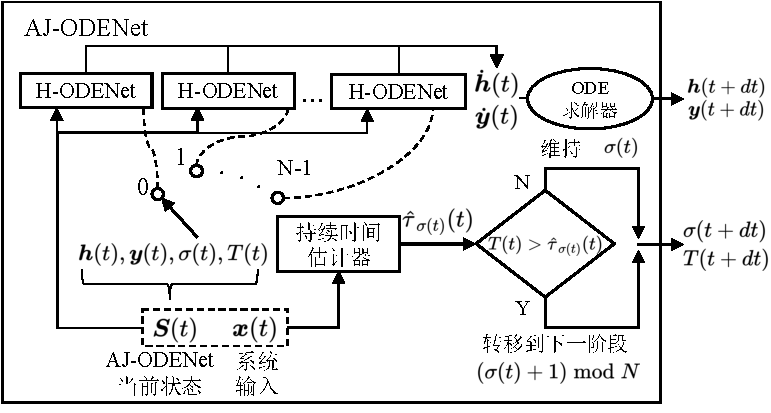
\includegraphics[width=0.8\textwidth]{figures/chapter4/Jump-ODEnet.pdf}
    \caption{AJ-ODEnet 模型结构}
    \label{fig:AJ_ODEs}
\end{figure}
在图\ref{fig:AJ_ODEs}中,AJ-ODEnet模型嵌入了$N$个H-ODEnet模块,根据状态变量$\sigma(t)$,在同一时刻只采用其中一个H-ODEnet模块用于系统预测。
。相比于普通的ODEnet仅建模隐状态的导数。
AJ-ODEnet将隐状态扩展为四个参数,从而覆盖连续时间跳变系统中输出变量变化以及阶段变量的变化。
其中,隐状态的计算和更新是连续时间域下的,表示为$\boldsymbol{S}(t) = [\boldsymbol h(t), \boldsymbol y(t), \sigma(t), T(t)]$,
其中四项分别为\textbf{系统隐状态}、\textbf{预测的系统输出}、\textbf{系统所处的当前阶段}和\textbf{处于当前阶段已经持续的时间}。
AJ-ODEnet可以看作是ODEnet的扩展形式,
计算更新过程可以视为给定时间点$t$ 和无穷小时间步长$\tau$计算微分方程的解,
如\equref{equa:states_updates}所示:

% For attention, even though there are several ODEnets as dynamical representations for available stages, only one ODEnet is active during processing, appointed by stage predictor. Therefore, AJ-ODEnet can still be seen as an extended version of ODEnet. Different to ODEnet shown in 式 \eqref{equ:ode_net} , which contains only self-governed hidden state predicted from input, AJ-ODEnet extend the hidden state to four arguments to cover enough dynamical variations in the system. Specifically, the calculation and update of hidden states are continuous-time processes, denoted by $\boldsymbol{S}(t) = [\boldsymbol h(t), \boldsymbol y(t), \sigma(t), T(t)]$, represent the \textbf{predicted hidden states}, \textbf{predicted system outputs}, \textbf{current stage} and \textbf{duration of current stage} respectively. %given current timestamp. 

% The updating can be seen as a differential process given time point $t$ and infinitesimal time step $\tau$, as illustrated by 式~(\ref{equa:states_updates}):

\begin{align}
\label{equa:states_updates}
\boldsymbol S(t+dt)=\left[
\begin{aligned}
&\left .\begin{aligned}
&\boldsymbol{h}(t) + \frac{d \boldsymbol{h}(t)}{\tau} *dt  \\
&\boldsymbol{y}(t) + \frac{d \boldsymbol{y}(t)}{\tau} *dt  \\
\end{aligned}
\right \}\quad \text{见公式} \eqref{equ:dh}\text{, }\eqref{equ:dyns}\text{, 和 }\eqref{equ:dys}
\\
&s(t+dt) =
\left\{
\begin{aligned}
\sigma(t) + 1 \text{ mod } N,\quad &T(t)>=\hat {\tau}_{\sigma(t)}(t) \\
\sigma(t), \quad &\text{else}
\end{aligned}
\right.\\
&T(t+dt) = 
\left\{
\begin{aligned}
0,\quad &T(t)>=\hat {\tau}_{\sigma(t)}(t) \\
T(t)+dt, \quad &\text{else}
\end{aligned}
\right.\\
\end{aligned}
\right]
\end{align}
\subsection{基于时间预测器的阶段自转移}
\label{sec:stage_trans_predic}

对于复杂的周期性多阶段系统而言,很难用统一的模型拟合系统的所有阶段,在长期预测问题中该问题更加明显。
对于周期稳定、各个阶段持续时间不变的系统,可以将系统的运行轨迹平均分解为若干区间,分别学习各阶段内的系统动态特性。
但是,更普遍的情况是,系统中各阶段的持续时间长度会受到系统内部和外部多个变量的影响。为了使模型适用于系统中各阶段持续时间不稳定的情况, 本章引入了“持续时间估计器”,通过学习的方式,在预测时预估每个阶段的持续时间,并辅助模型判断是否应切换到下一阶段。

具体地,我们结合周期性多阶段系统中的先验知识,可以很容易地设计一个状态转换过程描述系统在各个阶段之间的转换。
% 基于该AJ模型,可以建立一个基于持续时间估计器的阶段转换预测器。
从给定的数据集中学习相邻阶段之间的转换规则,使系统在运行时切换到不同的H-ODEnet进行预测,将系统输出预测和阶段识别进行解耦。

对于在$t$时刻的连续时间状态$\boldsymbol{S}(t) = [\boldsymbol{h}^T(t), \boldsymbol{y}^T(t), T(t), \sigma(t)]^T$ , 
$\sigma(t)\in\{0,\dots,N-1\}$表示系统当前所处阶段,$T(t)$表示系统处于阶段$\sigma(t)$的持续时间。

对于\equref{sec:stage_trans_predic}所述的状态演化过程,本章基于多层感知器实现了与当前阶段变量${\sigma(t)}$绑定的持续时间估计器$\hat{\tau}_{{\sigma(t)}}$来预测当前阶段的持续时间。预测器的输入为当前隐状态$\boldsymbol{h}(t)$和外部输入$\boldsymbol{x}(t)$:
% 对于系统运行过程中可能出现的每个阶段$\sigma(t)$,基于多层感知器分别构建持续时间预测器,预测器的输入为当前隐状态$\boldsymbol{h}(t)$和外部输入$\boldsymbol{x}(t)$。
% $\hat{\tau}_{\sigma(t)}$为持续时间估计器预估的$\sigma(t)$阶段将会持续的时间。
\begin{equation}
\hat{\tau}_{\sigma(t)}(t)=\text{NN}\left([\boldsymbol{h}(t), \boldsymbol{x}(t)], \phi_{\sigma(t)}\right)
\end{equation}
其中$\phi_{\sigma(t)}$为可学习参数,当满足$T(t)\geq\hat{\tau}_{\sigma(t)}(\boldsymbol{h}(t),\boldsymbol{x}(t))$时,模型将切换到下一阶段$(\sigma(t)+1)\text{ mod } N$并将$T(t)$复位为0。
% where $\phi_{\sigma(t)}$ is learnable parameters.
% % 图.re.~\ref{fig:dt_label} illustrates the predicting and supervised signals of duration time predictors.
% %the accumulative duration of current stage satisfies 
% $T(t)\geq\hat{\tau}_{\sigma(t)}(\boldsymbol{h}(t),\boldsymbol{x}(t))$, the model will switch to the next stage $(\sigma(t)+1)\text{ mod } N$ and reset $T(t)$ to zero.
\section{基于编码器解码器结构的微分方程网络初值估计与序列预测}
\label{sec:encoder_decoder}
% 求解ODE方程前,需要确定初值。
在周期跳变系统的开环预测问题中,确定系统当前所处的相位,即识别当前所处阶段以及当前阶段已经持续的时间,是极其重要的。
% Meanwhile, the observation space of complicated system is always incomplete, subject to the limitation of monitoring techniques. Thus, to make accurate prediction, the model needs to 
% infer the uncertain information by embedding the historical trajectories in the initial state.
与此同时,受限于测量技术及成本的限制,复杂工业系统的观测空间往往是不完备的。因此,为了实现精确的预测,模型需要对系统的非确定性进行推理。
本节将介绍如何根据给定条件范围下的序列数据推断系统的非确定性信息,并作为求解AJ-ODEnet所需的初始状态。

% 在对周期性多阶段系统进行长期预测时,确定系统当前的相位是至关重要的,包括确定系统当前处于哪个阶段以及当前阶段的持续时间。
% 同时,受系统观测空间的限制,建模预测复杂系统的可用数据大多是局部观测数据,系统的部分指标量是不可知的。
% 为了使预测结果更准确,模型需要从历史序列推断系统的不确定信息并将其嵌入在求解ODE方程的初始状态中。

% In long-term prediction for periodic system, it is critical to determine the current phase position, including identifying current stage and the lasting time of current stage.
% % This paper incorporates the historical trajectories to estimate the initial , the phase position and 
% In the meanwhile, the available data for modeling industrial system are mostly partial observations, subject to the limitation of observation space.
% To make accurate prediction, the model need to 
% %access historical system trajectories and 
% infer the uncertain information by embedding the historical trajectories in the initial state.
% % In the meanwhile, to make accurate prediction for high-order partially observed system with long time delay, AJ-ODEnet need to access historical information, which can be achieved by embedding the historical system trajectories in the initial state.
% Furthermore, the proposed H-ODEnet only models the derivatives of system outputs, $\dot{\boldsymbol{y}}(t)$,
% % It requires the initial system outputs when H-ODEnet is solved.
% the initial system outputs are required to be embedded in the initial state when solving H-ODEnet.
% % The initial system outputs should also be embedded in the initial state.

本章遵循~\cite{du2020multivariate,yuan2020dual}中引入的编码器-解码器框架,使用两个AJ-ODEnets
分别构建用于编码历史系统轨迹的编码器和预测系统输出的解码器,如图\ref{fig:AJ-ODEnet_framework}。
模型输入的时间序列数据包括条件范围$\{{\boldsymbol{Y}}_{t_{1}:t_{I}}, {\boldsymbol {X}}_{t_{1}:t_{I}}\}$和预测范围$\{{\boldsymbol {X}}_{t_{I+1}:t_{L}}\}$。
% The whole AJ-ODEnet framework is shown in 图.~\ref{fig:AJ-ODEnet_framework}, illustrates how data flows through the modules. 
\begin{figure*}[htb]
    \centering
    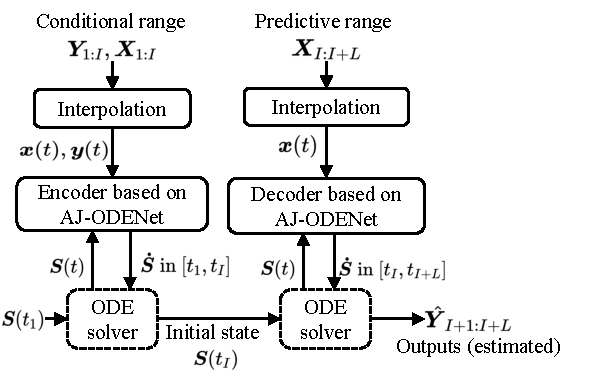
\includegraphics[width=\linewidth]{figures/chapter4/Jump-ODEnet_flow.pdf}
     \caption{基于AJ-ODEnet的编码器-解码器预测框架}
    % \caption{The data flow in AJ-ODEnet framework}
    \label{fig:AJ-ODEnet_framework}
\end{figure*}

由于ODEnet中求解微分方程需要连续的数据,所有范围的数据都需要先经过数据预处理转换为连续时间序列,利用编码器对条件范围内的数据进行编码,构建求解AJ-ODEnet解码器所需的初始状态$\boldsymbol S(t_I)$。
% be calculated in the end by solving 
% AJ-ODEnet encoder for the decoding phase. 
%conditional data range in $[t_1,t_I]$ contains the operational information of system and the initial state $\boldsymbol S(t_I)$ for decoding phase will be calculated at the end of conditional range by solving AJ-ODEnet encoder. 

在条件范围内,根据初始状态$\boldsymbol S(t_1)$,求解AJ-ODEnet编码器对应的常微分方程,可以得到$t_I$时刻的状态$\boldsymbol S(t_I)=[\boldsymbol h(t_I), \boldsymbol y(t_I), s(t_I), T(t_I)]^T$。
然后在预测阶段,基于AJ-ODEnet的解码器将会根据初始状态${\boldsymbol{S}}_I$和系统外部输入$\{{\boldsymbol {X}}_{t_{I}:t_{I+L}}\}$估计预测范围下隐状态的导数,进而预测系统输出。

具体来说,在条件范围$[t_1, t_I]$的编码阶段,我们将连续时间信号$\boldsymbol y(t)$和$\boldsymbol x(t)$合并起来作为AJ-ODEnets编码器的输入,生解码器所需的初始状态,如式~\eqref{equa:initial_state}所示。
% % Expect for $\boldsymbol h(t)$, the rest three parts are unrelated to the encoder AJ-ODE-nets because they can be estimated from data in conditioning range directly.
% Specifically, in encoding phase for conditional range $[t_1, t_I]$, we concatenate the continuous time signal $\boldsymbol y(t)$ and $\boldsymbol x(t)$ as the inputs of AJ-ODE-nets encoder to generate initial state of predictive decoder ODE-nets, as shown in 式~\eqref{equa:initial_state}.

\begin{equation}
\boldsymbol{\tilde S}(t_I)=\text{ODESolve}(\text{Encoder AJ-ODE-nets},\boldsymbol S(t_1)
, 
\left [
\begin{aligned} 
&\boldsymbol {x}(t) \\
&\boldsymbol {y}(t)
\end{aligned}
\right ]
, t_1, t_I)
\label{equa:initial_state}
\end{equation}

其中$t_1$时刻的初始状态定义为:
$
\boldsymbol S(t_1)=\left[\boldsymbol h(t_1) = \boldsymbol 0,\boldsymbol y(t_1),T(t_1)=0,s(t_1)\right ]^T
$。 
根据求解得到的
$\boldsymbol{\tilde{S}}(t_I)=[\boldsymbol{\tilde h}(t_I), \boldsymbol{\tilde y}(t_I), \tilde s(t_I), \tilde T(t_I)]^T$。
可以获得状态$\boldsymbol{S}(t_I)=[\boldsymbol{h}(t_I), \boldsymbol{y}(t_I), \tilde s(t_I), \tilde T(t_I)]^T$
$\boldsymbol{h}(t_I)$ 是从均值为$\boldsymbol{\tilde h}(t_I)$,协方差矩阵为单位矩阵$\boldsymbol I$的对角多元高斯分布中采样得到的。
% where the initial state is defined as:
% $
% \boldsymbol S(t_1)=\left[\boldsymbol h(t_1) = \boldsymbol 0,\boldsymbol y(t_1),T(t_1)=0,s(t_1)\right ]^T
% $. 
% % The initial system outputs, $\boldsymbol y(t_0)$ are estimated from nature spline interpolation.
% According to the solved $\boldsymbol{\tilde{S}}(t_I)=[\boldsymbol{\tilde h}(t_I), \boldsymbol{\tilde y}(t_I), \tilde s(t_I), \tilde T(t_I)]^T$, the state $\boldsymbol{S}(t_I)$ is obtained by sampling $\boldsymbol{h}(t_I)$ from a diagonal multivariate normal distribution whose mean and covariance matrix are $\boldsymbol{\tilde h}(t_I)$ and identity matrix $\boldsymbol I$.
%and copying $\boldsymbol{\tilde y}(t_I), {\tilde s}(t_I), {\tilde T}(t_I)$.
由于在网络传播过程中存在采样操作。为了构建用于梯度传导的计算图以及减小训练时梯度估计的方差,上述采样过程使用了重参数化法\cite{kingma2013auto}。

本节设计AJ-ODEnets编码器的最重要的目的是估计隐变量$\boldsymbol h(t_I)$。上述从概率分布中采样的方式相当于将$\boldsymbol h(t)$视为条件序列生成模型中的隐变量,从过去的系统输出和输入中推测隐变量的近似状态后验\cite{10.5555/3454287.3454765,Hafner2019}。

接下来,通过给定解码阶段的初始状态$\boldsymbol S(t_I)$ 和连续时间系统输入$\boldsymbol x(t)$,在$[t_I, t_{I+L}]$范围内求解AJ-ODEnet解码器对应的常微分方程,可以得到预测范围内的隐变量状态$\boldsymbol S(t)$,其中包括系统在任意时刻$t_i$的系统输出$\boldsymbol{\hat{y}}(t_i)$:
\begin{equation}
\boldsymbol {\hat S}(t_{I+L})=\text{ODESolve}(\text{AJ-ODEnet Decoder},\boldsymbol S(t_I)
, \boldsymbol {x}(t), t_I, t_{I+L})
\label{equ:decoding}
\end{equation}
% With solving the , the predicted system outputs $\boldsymbol \hat{y}(t_i)$ at arbitrary time points $t_i$, where $i\in \{I, I+1, \cdots, I+L\}$
% When the AJ-ODEnet decoder is being solved 

%where $i\in \{I, I+1, \cdots, I+L\}$ corresponds to the predicted indices, 
%At an arbitrary time point $t_i$, the predicted system outputs $\boldsymbol{\hat{y}}(t_i)$ are also obtained accompanied with solving the AJ-ODEnet decoder.

% In addition to embedding the system outputs $\boldsymbol y(t)$ in ODE inputs, a slight difference between AJ-ODE-nets encoder and AJ-ODE-nets decoder is that 

AJ-ODEnets编码器和AJ-ODEnets解码器之间有两个区别。首先,系统输入$\boldsymbol x(t)$和输出$\boldsymbol y(t)$都均是编码阶段的输入,而解码器的输入仅包含系统输入$\boldsymbol x(t)$。因此解码器和编码器中H-ODENet的输入层的大小是不一致的。
其次,对于条件范围下的编码过程来说,由于系统的输入输出数据已知,模型进行阶段转移时,可直接根据系统先验属性得到阶段之间的转换规则,不需要阶段转换预测器进行阶段的自转移。
对于解码器,由于系统输出$\boldsymbol y(t)$未知,因此需要利用阶段转换预测器进行状态自切换。
这两个区别表明,在求解初始状态的过程中,编码器不引入阶段转换预测器,而是根据实际的系统输出准确地识别系统当前所处的阶段,并推导出$S(t_I)$,$T(t_I)$ 和$y(t_I)$。因此,初始状态$S(t)$中的$\sigma(t)$和$T(t)$是准确可靠的。
对于解码器来说,相邻阶段之间的转移是依靠持续时间预测器进行判断,无法保证绝对准确的。在长范围开环预测时会带来较大的累积相位误差。
\section{模型训练}
\label{sec:loss_function}
% AJ-ODEnet describes an ODE equation defined on an increasing continuous-time state $\boldsymbol{S}(t) = [\boldsymbol{h}^T(t), \boldsymbol{y}^T(t), T(t), s(t)]^T$.
% In prediction range, system outputs is predicted by solving the ODE equation and extracting the second part of system state, $\boldsymbol{y}^T(t_x)$ at any time $t_x$.
% The following paragraphs will present detailed definition of continuous-time state and their derivative of time $\hat{\boldsymbol{S}}(t)$.
利用AJ-ODENet编码器根据条件范围下的序列输入数据获得初始状态后,在预测范围下求解AJ-ODEnet解码器即可得到预测结果$\hat{\boldsymbol{Y}}_{t_{I+1}: t_{I+O}}$。利用数据集中真实的系统输出序列即可通过有监督学习的方式对网络进行端到端的训练。接下来本小节将对损失函数的定义进行介绍。

在所述的编码器解码器框架中,待训练的参数包括三部分:$\boldsymbol \zeta=\{\boldsymbol{\Theta}_d, \boldsymbol{\Theta}_e,\boldsymbol{\Phi}\}$
% After obtaining initial states through the conditional data range,
% %By solving AJ-ODEnet encoder, the sequential inputs $\boldsymbol{Y}_{t_{1}: t_{I}}, \boldsymbol{X}_{t_{1}: t_{I}}$ is encoded to the initial state, $\boldsymbol{S}\left(t_{I}\right)$, for Prediction-AJ-ODEnet.
% next, the predicted results of range $ \hat{\boldsymbol{Y}}_{t_{I+1}: t_{I+O}}$ are obtained by solving AJ-ODEnet decoder based on the inputs of the same range: $\boldsymbol{X}_{t_{I}: t_{I+O}}$.
% % Two phases construct the computational graphs based on parameterized neural networks, which will be backpropagated for training.
% % The complete parameters, $\boldsymbol \zeta=\{\boldsymbol{\Theta}_d, \boldsymbol{\Theta}_e,\boldsymbol{\Phi}\}$, will be trained in end to end manner, including three parts:
% The complete parameters, $\boldsymbol \zeta=\{\boldsymbol{\Theta}_d, \boldsymbol{\Theta}_e,\boldsymbol{\Phi}\}$, include three parts:
\begin{itemize}
    \item $\boldsymbol{\Theta}_e=\{\theta_i^{\mathcal{Y}^{ns}},\theta_i^{\mathcal{Y}^{ns}},\theta_i^{\mathcal{H}}\}_{i=0}^{N-1}$: 在AJ-ODEnet编码器中的$N$个H-ODEnet 
    \item $\boldsymbol{\Theta}_d=\{\theta_i^{\mathcal{Y}^{ns}},\theta_i^{\mathcal{Y}^{ns}},\theta_i^{\mathcal{H}}\}_{i=0}^{N-1}$: 在AJ-ODEnet解码器中的$N$个H-ODEnet 
    \item $\boldsymbol{\Phi}=\{\phi_i\}_{i=0}^{N-1}$:  AJ-ODEnet解码器中的$N$个持续时间预测器。
\end{itemize}
为了能够以端到端的方式对上述参数进行训练。需要优化的模型损失函数包括两部分,分别为模型预测系统输出的误差损失$\mathcal{L_P}$和持续时间预测器预测的各阶段持续时间的误差损失$\mathcal{L_{\tau}}$:
\begin{equation}
\mathcal{L}(\boldsymbol{\Theta}_e, \boldsymbol{\Theta}_d, \boldsymbol \Phi) = \mathcal{L_P}(\boldsymbol{\Theta}_e, \boldsymbol{\Theta}_d) + \lambda\mathcal{L_{\tau}}(\boldsymbol \Phi)
\end{equation}
其中$\lambda$是平衡$\mathcal{L_P}$和$\mathcal{L_{\tau}}$的权重参数。

对于$\mathcal{L_P}$,由于模型将$\boldsymbol h(t_I)$作为隐变量进行后验推断,因此可以采用变分贝叶斯优化的方法,将最大化系统观测输出的证据下界\textit{Evidence lower bound} (ELBO) (ELBO)作为模型训练的目标,以近似地最大化系统输出的边际似然\cite{10.5555/3454287.3454765}:
% For the part of $\mathcal{L_P}$, by considering $\boldsymbol h(t_I)$ as a latent variables, 
% %$\mathcal{L_P}$ is the defined as the \textit{Evidence lower bound} on the marginal likelihood of system outputs:
% we hope to maximize the \textit{Evidence lower bound} (ELBO) on the marginal likelihood of system outputs\cite{10.5555/3454287.3454765}:
\begin{equation}
\begin{aligned}
&\operatorname{ELBO}(\boldsymbol{\Theta}_e,\boldsymbol{\Theta}_d)=-\operatorname{KL}\left[q_{\boldsymbol \Theta_e}(\boldsymbol h({t_I}) \mid\boldsymbol{Y}_{t_{1}: t_{I}}, \boldsymbol{X}_{t_{1}: t_{I}}) \| p\left(\boldsymbol h({t_I})\right)\right]+\\&\mathbb{E}_{\boldsymbol h({t_I}) \sim q_{\boldsymbol \Theta_e}(\boldsymbol h({t_I}) \mid\boldsymbol{Y}_{t_{1}: t_{I}}, \boldsymbol{X}_{t_{1}: t_{I}})}\log p_{\boldsymbol \Theta_d}(\{\boldsymbol y_{t_i}\}_{i=I+1}^{I+L}\mid \boldsymbol h_{t_I},\boldsymbol X_{t_I:t_{I+L}})
\end{aligned}
\end{equation}
在本研究中,我们参考前人的工作~\cite{chen2018neural, 10.5555/3454287.3454765, Yildiz2019},对隐变量的先验分布和后验分布做出了如下假设。
我们假设隐变量$p(\boldsymbol{h}(t_I))$的先验分布服从正态分布$\text{Normal}(\boldsymbol{h}(t_I);\boldsymbol 0, \boldsymbol I)$。模型估计的后验分布$q_{\boldsymbol \Theta_e}(\boldsymbol h({t_I}) \mid\boldsymbol{Y}_{t_{1}: t_{I}}, \boldsymbol{X}_{t_{1}: t_{I}})$为对角多元高斯分布。
由此,KL散度项可以简化为对于$\boldsymbol h(t_I)$的正则项。
对于解码器部分,我们定义生成模型$p_{\boldsymbol \Theta_d}({\boldsymbol Y}_{I+1: I+L}\mid \boldsymbol h_{t_I},\boldsymbol X_{t_I:t_{I+L}})$为具有固定协方差矩阵的正态分布。
分布的均值定义为AJ-ODEnet解码器预测出的系统输出。最大化重构似然的期望$\mathbb{E}_{q_{\boldsymbol \Theta_e}(\boldsymbol h_{t_I} \mid\cdots)}\left[\log p_{\boldsymbol \Theta_d}({\boldsymbol Y}_{I+1: I+L}\mid \boldsymbol h_{t_I},\boldsymbol X_{t_I:t_{I+L}})\right]$可以简化为最小化系统输出预测值$\hat{\boldsymbol Y}_{I+1: I+L}$与实际系统输出${\boldsymbol Y}_{I+1: I+L}$之间的$L^2$距离。综上所述,预测系统输出的损失和编码获得隐变量的损失可表示为:

% In this study, we refer to the previous works~\cite{chen2018neural, 10.5555/3454287.3454765, Yildiz2019} and make the following assumptions to regulate the training of loss functions.
% We assume that the prior distribution of latent state $p(\boldsymbol{h}(t_I))$ obeys $\text{Normal}(\boldsymbol{h}(t_I);\boldsymbol 0, \boldsymbol I)$. 
% The posterior distribution $q_{\boldsymbol \Theta_e}(\boldsymbol h({t_I}) \mid\boldsymbol{Y}_{t_{1}: t_{I}}, \boldsymbol{X}_{t_{1}: t_{I}})$ is considered as a diagonal multivariate normal distribution whose covariance matrix is an identity matrix. 
% The KL divergence term could be simplified as a regularization item of $\boldsymbol h(t_I)$.
% For the decoder part, we define the generative model $p_{\boldsymbol \Theta_d}({\boldsymbol Y}_{I+1: I+L}\mid \boldsymbol h_{t_I},\boldsymbol X_{t_I:t_{I+L}})$ as a normal distribution with a fixed covariance matrix.
% And the mean of the distribution is defined as the predicted system outputs of AJ-ODEnet decoder.
% maximizing the expected reconstruction likelihood $\mathbb{E}_{q_{\boldsymbol \Theta_e}(\boldsymbol h_{t_I} \mid\cdots)}\left[\log p_{\boldsymbol \Theta_d}({\boldsymbol Y}_{I+1: I+L}\mid \boldsymbol h_{t_I},\boldsymbol X_{t_I:t_{I+L}})\right]$ could be simplified as minimizing $L^2$ distance between predicted system outputs $\hat{\boldsymbol Y}_{I+1: I+L}$ and real system outputs ${\boldsymbol Y}_{I+1: I+L}$.
% To sum up, the loss on predicting system outputs and loss on encoding are expressed as:
% \begin{equation}
% \begin{aligned}
% \mathcal{L_P}(\boldsymbol{\Theta}_e,\boldsymbol{\boldsymbol \Theta}_d)&=-\operatorname{ELBO}(\boldsymbol{\Theta}_e,\boldsymbol{\Theta}_d)\\
% &=||\boldsymbol h(t_I)||^2 + \sum_{i=I+1}^{I+L}\mid\mid\hat{\boldsymbol y}(t_i)-{\boldsymbol y}(t_i)\mid\mid^2
% \end{aligned}
% \end{equation}
\begin{equation}
\mathcal{L}_{\mathcal{P}}\left(\boldsymbol{\Theta}_{e}, \boldsymbol{\Theta}_{d}\right) =-\operatorname{ELBO}\left(\boldsymbol{\Theta}_{e}, \boldsymbol{\Theta}_{d}\right)
=\left\|\boldsymbol{h}\left(t_{I}\right)\right\|^{2}+\sum_{i=I+1}^{I+L}\left\|\hat{\boldsymbol{y}}\left(t_{i}\right)-\boldsymbol{y}\left(t_{i}\right)\right\|^{2}
\end{equation}

阶段持续时间预测器的误差损失$\mathcal{L}_{\tau}$定义为训练时每个阶段下,预测器估计的持续时间与该阶段实际持续时间之间的平均平方误差。
构建过程如图\ref{fig:dt_label}所示:
\begin{figure}
    \centering
    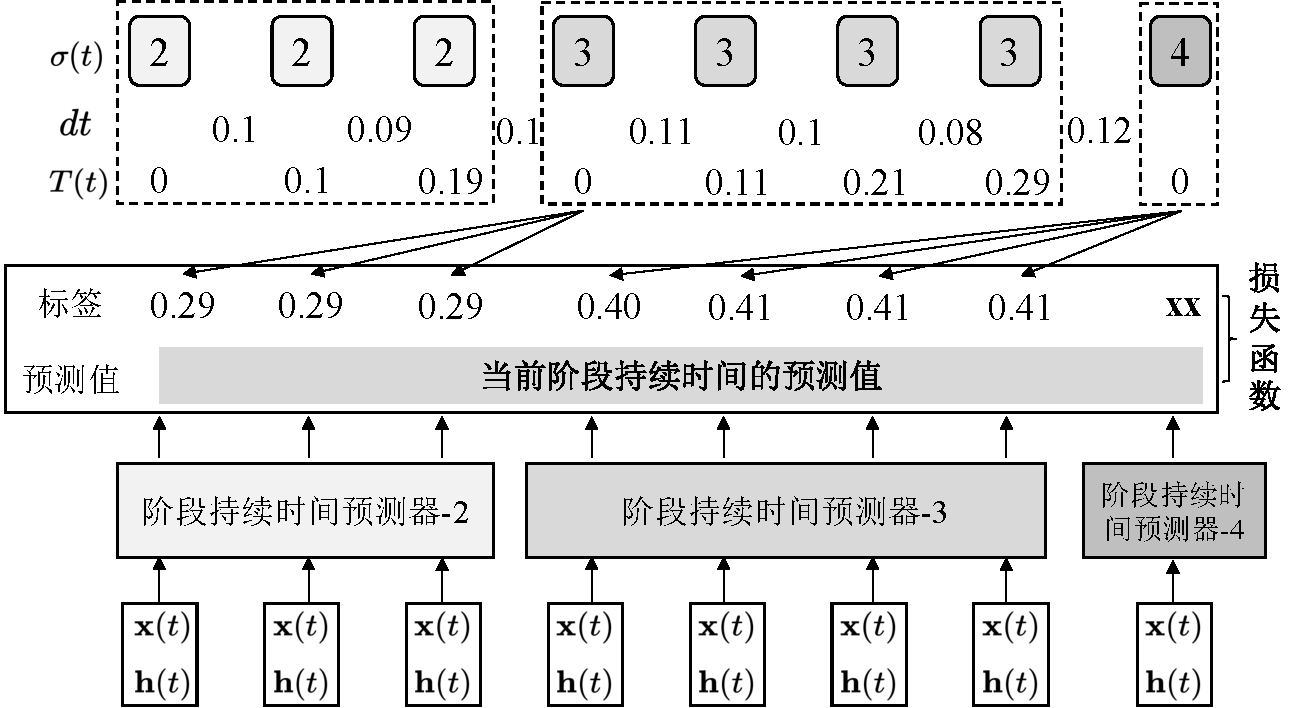
\includegraphics[width=0.8\linewidth]{figures/chapter4/dt_label.pdf}
    \caption{时间预测器的损失函数定义}
    \label{fig:dt_label}
\end{figure}
% \begin{equation}
%     \mathcal{L_P}(\boldsymbol \Theta) = ||\boldsymbol h(t_I)||^2 + \sum_{x=I+1}^{O}\mid\mid\hat{\boldsymbol y}(t_x)-{\boldsymbol y}(t_x)\mid\mid^2
% \end{equation}
\begin{equation}
    \mathcal{L_{\tau}}(\boldsymbol \Phi) =\sum_{i=I+1}^{I+L} \mid\mid\hat{\tau}_{s(t_i) }(t_i)-\tilde {\tau}(t_i))\mid\mid^2
\end{equation}
其中$\tilde {\tau}(t_i)$代表阶段$\sigma(t_i)$的持续时间,
为了计算$\tilde {\tau}(t_i)$,需要找到$t_i$所处阶段的区间边界$t_l$和$t_r$。
$t_r$为$[t_i, \infty)$]范围下,满足条件$\sigma(t_r)=\sigma(t_i)$且$\sigma(t_r+dt)\neq \sigma(t_i)$的最小值。
$t_l$为$(-\infty, t_i]$范围下,满足条件$\sigma(t_l)=\sigma(t_i)$且$\sigma(t_l-dt)\neq \sigma(t_i)$的最大值。
实际的阶段持续时间即为$\tilde {\tau}(t_i)=t_r-t_l$.


完整的网络模型通过Adam优化器进行训练。
完整的训练算法如算法\ref{alg:training}所示。
% where $\tilde {\tau}(t_i)$ represents the duration time of stage $s(t_i)$. 
% It is determined by finding the minimal $t_r$ in range$[t_i, \infty)$, 
% which satisfies $s(t_r)=s(t_i)$ and $s(t_r+dt)\neq s(t_i)$, and the maximum $t_l$ in range $(-\infty, t_i]$, which satisfies $s(t_l)=s(t_i)$ and $s(t_l-dt)\neq s(t_i)$.
% The real duration is obtained as $\tilde {\tau}(t_i)=t_r-t_l$.

% The entire network is trained with Adam optimizer. 
% The overall training algorithm is illustrated in Algorithm \ref{alg:training}.
\floatname{algorithm}{算法}  
\begin{algorithm*}[]
\caption{ 基于AJ-ODEnets的编码器-解码器训练过程 }
\label{alg:training}
\begin{algorithmic}[1]
\For{每一个训练轮次}
\For{$k$ steps}
\State  在训练集$S$中随机抽样一批序列 $\{\boldsymbol{Y}_{1:I+L}, {\boldsymbol {X}}_{1:I+L}\}$.
\State \text{//}\textit{为了加快训练速度,下面的步骤是并行执行的.}
\State 给训练数据的各阶段打标签: $s_{t_1:t_{I+L}}$
\State 使用样条插值来处理离散序列${\boldsymbol {X}}_{1:I+L}$, $\boldsymbol{Y}_{1:I+L}$,生成$[t_1, t_{I+L}]$的连续序列 $\boldsymbol X(t)$ 和$[t_1, t_{I}]$的连续序列 $\boldsymbol Y(t)$。
\State 编码阶段: AJ-ODEnet编码器根据条件范围下的系统输入和输出序列估计初始状态 $\boldsymbol{S}\left(t_{I}\right)$,\eqref{equa:initial_state}。
\State 预测阶段: AJ-ODEnet解码器根据预测范围下的系统输入 $[t_I, t_{I+L}]$预测离散时间点$\{t_{I+1}, \dots, t_{I+L}\}$下的系统输出,\eqref{equ:decoding}。
\State 利用随机梯度 $\nabla_{\boldsymbol{\Theta_{e}}, \boldsymbol{\Theta_{d}}, \boldsymbol \Phi}\mathcal{L}\left(\boldsymbol{\Theta}_{e}, \boldsymbol{\Theta}_{d}, \boldsymbol{\Phi}\right)$更新两个AJ-ODEnet中的参数 $\boldsymbol{\Theta_{e}}, \boldsymbol{\Theta_{d}}, \boldsymbol \Phi$:
\EndFor
\EndFor
\end{algorithmic}
\end{algorithm*}


\section{周期性制冷系统预测仿真及系统优化}
\label{sec:evalutaion}
接下来本章将使用AJ-ODENet模型及衍生出的编码器解码器预测框架解决某工业制冷系统的建模及预测问题,并采用两个实验探究模型的预测效果并基于仿真模型给出制冷系统的运行优化策略。
具体地,在第一个实验中,我们使用AJ-ODENet模型根据当前的负载功率和环境温度,在线预测制冷系统的输出量。
在第二个实验中,依托于实验一中训练得到的预测仿真模型,实现对不同制冷启动温度配置下的制冷功耗进行仿真,并结合仿真结果给出制冷策略优化。
接下来本章将首先介绍作为实验对象的制冷系统,然后介绍模型的训练参数、评估结果和预测仿真结果。

% In this section, we show the framework construction in an use case, by applying it to a real cooling system of a data center, with two case studies. Prior knowledge in this case refers to the cooling configuration, output constraints to guide the design and improve the prediction accuracy. The objective of the first implementation is to predict in real time the energy consumption of cooling, based on current IT activities and environmental conditions. Based on the first model, the second case study optimizes the energy consumption by adjusting the temperature set point according to simulations. This realization makes use of the mechanism that prior knowledge is written into the AJ transformation rules. The following subsections details the model design, evaluation results and simulation results, starts by a background introduction about the cooling system.

\subsection{制冷系统简介}
% \subsection{Backgrounds about the studied cooling system}
\label{sec:ecotype_description}

实验中探究的制冷系统为施耐德电气公司~\cite{InrowACRD602}设计。
制冷系统为某一大型熔炼设备提供压缩制冷。
% 计算中心的集群为Grid5000大规模分布式集群,为在校科研人员提供CPU计算资源。
制冷系统的运行数据可通过调用Seduce平台~\cite{SeducePastor2018}的API获取数据。
Seduce平台是用于电源和温度管理的物联网平台,该系统以1hz的频率采集传感器监测数据,包括能耗和温度数据。
图~\ref{fig:inrow_3dArchitecture}展示了制冷系统提供热交换制冷的过程示意图。
该制冷系统包括室内和室外两部分。室内部分的主要模块为液体-空气热交换器,该模块吸收生产设备产生的热空气,然后通过管道、冷凝器和风机将热量转移和疏散到室外,通过压缩生成的冷空气输送至室内。

\begin{figure*}[!htbp]
  \centering
  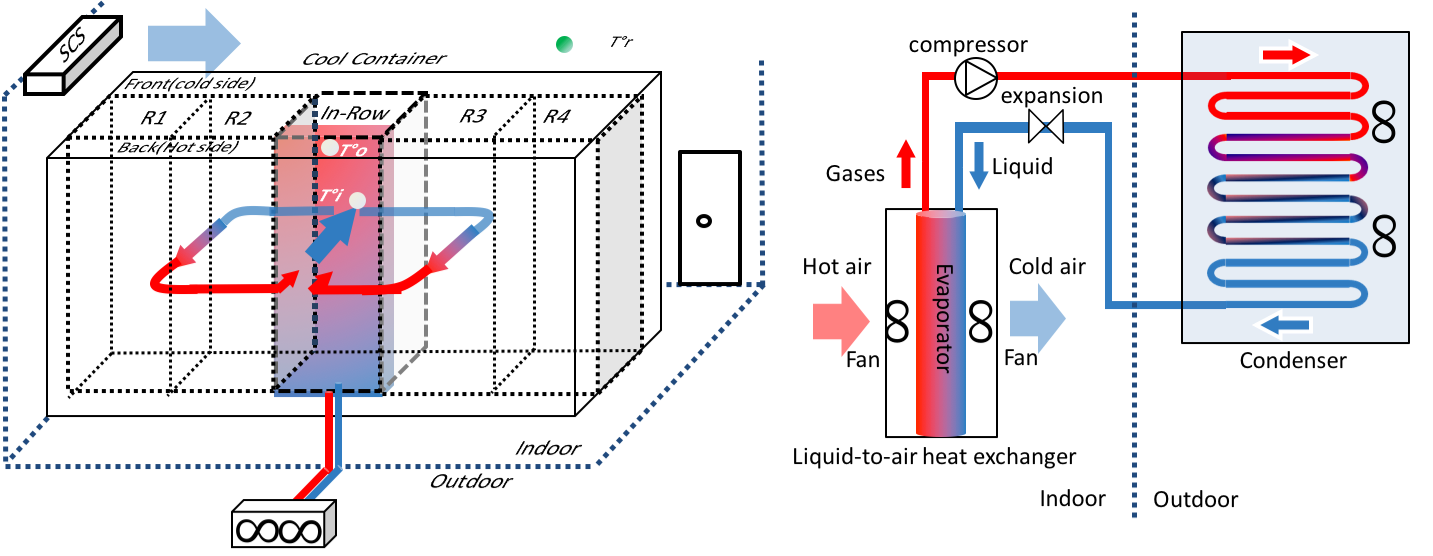
\includegraphics[width=0.8\textwidth]{figures/chapter4/inrow_architecture.png}
  \caption{工业制冷系统整体结构及热交换过程}
% \caption{Architecture of In-Row cooling module, position of heat eschanger, indoor and outdoor parts}
\label{fig:inrow_3dArchitecture} 
\end{figure*}

制冷系统作为常见的工业设施,是一种典型的周期性多阶段系统,其运行过程为部分可观测的2输入3输出(Multi-Input Multi-Output, MIMO)系统。
% In this modeling case study, cooling system is a typical periodic multi-stage system of an industrial infrastructure, it can be regarded as a partially observed MIMO (Multiple-Input Multiple-Output) system. 
直观地,热负载(熔炼设备的运行总功率($x_1(t)$))的升高会导致制冷系统进气口温度($y_3(t)$)升高。
另外,由于制冷系统和室外环境之间存在热交换,系统所处环境的温度($x_2(t)$)也会影响制冷系统的工作情况。
为了保持生产过程安全稳定运行,制冷系统需要维持室内的进气空气温度限定某预先设定的区间上下限内。
当进气口空气温度达到上限时,制冷系统会开启压缩机,制冷系统产生的制冷量($y_2(t)$)增加。当进气口温度温度低于设定值时,压缩机关闭,制冷系统变为待机状态。系统在压缩制冷时的运行功率($y_1(t)$)远大于关闭压缩机时的功耗。
伴随着制冷与待机,制冷系统的运行过程具有典型的周期多阶段特性,其阶段转换如图~\ref{fig:cooling_workloop}所示。 
% Intuitively, heat load of the date center, represented by total server power ($x_1(t)$), leads to the increase of inlet temperature ($y_3(t)$). The room temperature ($x_2(t)$) also affects the thermal system due to heat exchange between cooling enclosure and the room. The configurations of cooling system determine the upper and lower bounds of inlet temperature to keep appropriate operational temperatures for servers. 
%Once the compressor is on, cooling ability of heat exchanger will be enhanced and has more cooling production ($y_2(t)$) until inlet temperature decreases to the setting value, and accordingly, the system consumes more power ($y_1(t)$) than the compressor is off. Vice versa, the cooling system works based on the configurations in a infinite loop, as shown in 图.~\ref{fig:cooling_workloop}. 

当制冷系统待机时,进气口温度不断上升,其制冷量和制冷功率接近于0。
当制冷系统工作时,进气口温度不断下降,制冷量和制冷功率经过两个阶段的快速震荡后会趋近于某固定值。
因此,对于该制冷系统,实时功率消耗$y_1(t)$和实时制冷量$y_2(t)$为系统的稳定输出$\boldsymbol y_s(t)=[y_1(t), y_2(t)]$。
进气口温度$y_3(t)$为系统的非稳定输出:$\boldsymbol y_{ns}(t)=[y_3(t)]$。
将进气口温度定义为非稳定过程,这一性质与系统的先验特性是保持一致的。在第二个实验中,我们通过改变温度阈值而优化制冷系统能耗,需要模型对于进气口温度实现外推预测,在H-ODENet模型中将进气口温度定义为非稳定过程,对于实现可靠、合理的外推预测具有重要意义。

% In the H-ODEnet, $y_1(t)$ and $y_2(t)$ are defined as stationary outputs $\boldsymbol y_s(t)=[y_1(t), y_2(t)]$. The inlet temperature $y_3(t)$ is defined as non-stationary outputs $\boldsymbol y_{ns}(t)=[y_3(t)]$.
% By modeling the inlet temperature change as a non-stationary process, the temperature will climb steadily when cooling system is off and vice versa when cooling system is on.
% This property is consistent with the prior knowledge of system and important for subsequent experiments about the optimizations of temperature thresholds.


\subsection{数据预处理:离散序列插及阶段标注}

为了使用微分方程网络对序列数据进行处理,需要使用插值方法将带有缺失值的不规则采样数据集转换为连续信号。
在本章实验环节中,制冷系统数据集存在采样间隔不均匀、部分数据缺失的问题。本章参照前人工作\cite{kidger2020neural},使用三次样条插值方法对离散时间序列$\boldsymbol X_{[1:I+L]}$和$\boldsymbol Y_{[1:I]}$进行插值,构成连续时间信号$\boldsymbol Y:[t_1,t_{I}]$和$\boldsymbol X:[t_1,t_{I+L}]$。在任意时刻$t$,  $\boldsymbol X(t)$和$\boldsymbol Y(t)$二阶可微,满足自适应步长求解器求解神经ODE系统时所需的必要条件\cite{kidger2020neural}。
当待处理的数据集包含的噪声比较少时,相比于其他插值算法,三次样条插值实现简单,且对原始
序列数据的破坏较小,插值生成的连续信号中的噪音较小。
% First part in preprocessing module mentioned in~\ref{sec:data_prepocessing_module} concerns the choice of interpolation method to transfer the input data sets with irregular missing values to continuous ones. In this concrete case, the data sets of cooling system come from highly reliable and well calibrated sensory measurement system, which works in relatively stable environment. Following the previous study in \cite{kidger2020neural}, natural cubic spline is usually employed to generate continuous-time processes  $\boldsymbol Y:[t_1,t_{I}]$ and $\boldsymbol X:[t_1,t_{I+L}]$ from discrete-time sequences $\boldsymbol X_{[1:I+L]}$ and $\boldsymbol Y_{[1:I]}$.
% For an arbitrary time point $t$, the path $\boldsymbol X(t)$ and $\boldsymbol Y(t)$ are second order differentiable functions, which is a necessary condition of employing adaptive step size solvers to solve the neural ODE system.
% When dealing with dataset containing not much noisy data, compared with other options for interpolation, natural cubic splines give essentially the minimum regularity. In this case, the data suffers little noise disturbance, spline interpolation is the appropriate choice in dealing with these cooling system operational data sets. 
% The second part is sliding, 
%It is a fortunate fact that our cooling system works in a closed space and suffers very little noise disturbance from environment.

接下来,为了训练AJ-ODEnet模块中的阶段转换预测器,需要为序列数据标注各时间点所属的阶段。我们基于系统的先验知识构建了用于描述系统阶段转换的状态转换过程,并基于此自动地为序列数据标记所属阶段。

根据现场观察和对于制冷系统的了解,可知的系统先验知识如下:
\begin{itemize}
    \item 根据当前进气口温度以及启停设定值,制冷系统的工作模式在压缩机启动和压缩机关闭两种状态之间来回切换。
    \item 系统包含有四个可观测的工作阶段,每个阶段下,系统输出呈现不同的动态特性。
    % \item 系统周期性循环运行,一个周期包含四个操作阶段。
    % \item 监测的系统输出值:进气口温度、制冷量和系统功率受到设置的进气口温度上下限的限制。
\end{itemize}

% According to the observations in site and the pre-defined configurations, some knowledge are known in prior: 
% \begin{itemize}
%     \item Cooling system is running with respect to natural laws and energy balance.
%     \item These physical processes are mixed with stationary and non-stationary properties.
%     \item The system runs in periodic loops, one loop contains four operational stages.
%     \item The outputs of the system monitored here: inlet temperature, cooling production and power are constrained between upper and lower bounds based on the configurations.
% \end{itemize}
% The descriptions of each stage along with the transformation rules are detailed in Tab.~\ref{tab:cooling_dfa}.
% 图.~\ref{fig:stages_mark} demonstrates the auto labeling results with an example: 
根据上述先验知识,我们精确地定义了系统的各个阶段并给出了阶段之间的转换规则,如表~\ref{tab:cooling_dfa}所示。
% 每个时刻 $t_i$的阶段变量 $s(t_i)\in\{0,\dots,N-1\}$。
制冷系统的运行阶段在$N=4$个阶段之间依周期地循环切换。
% 在下面的图中,为了更好地区分各个阶段,四个阶段内的原始数据或预测数据将被标记为不同的颜色。
%Two stages \textit{On} and \textit{Off} are relatively longer and the other stages are short-lived.
% The AJ transformation rules are designed as well according to prior knowledge mentioned above.
% % 图.~\ref{fig:dt_label} illustrates three duration estimators estimating the duration individually in corresponding stage. In the figure, $dt$ represents the sampling interval and $T(t)$ denotes the duration. The learning of duration estimator is supervised by \textit{Label} which is inferred from time points when stages transform. 
% Formally, the stage variable of each sample $t_i$ are written as $s(t_i)\in\{0,\dots,N-1\}$. 
% The cooling system runs periodically, the stage variable $s(t)$ moves around in a loop of size $N=4$.
% In the following graphs, the four stages are marked with different colors for better illustration.
% %In the following graphical illustrations, the four stages are marked with different colors for visualizing the stage belongs to at current timestamp.
% %The transform rules in Table.~\ref{tab:cooling_dfa} are deterministic and can be easily implemented by programming, so there is no need for manual marking in the phase of generating stage labels.
在图\ref{fig:state}中,我们统计了在不同的热负载下,每次\textit{On}阶段和\textit{Off}阶段的持续时间的分布情况。
结果表明,阶段持续时间与服务器负载功率值有较强相关性。在特定的热负载下,阶段持续时间${\tau}_{i}$的分布趋于稳定。
这一结果说明利用系统的热负载输入以及环境温度预测各个阶段的持续时间是具有可行性的。
% 与服务器负载功率值有较强相关性,特定数据集下的阶段持续时间分布相对稳定。
% In 图.~\ref{fig:state}, we analyse the statistical properties of duration in each stage. 
% It demonstrates that the distribution of duration ${\tau}_{i}$ is stationary and highly depends on the nearby external inputs.
\begin{figure}
\centering
\hspace{-0.1in}
\subfigure[阶段-\textit{关闭}]{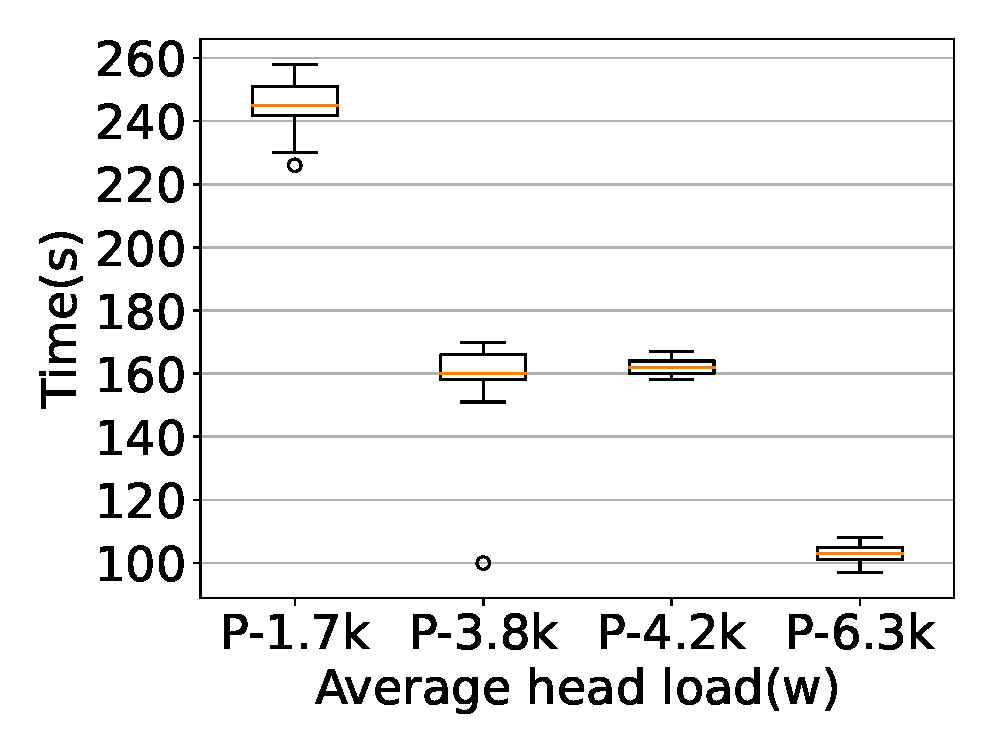
\includegraphics[width=0.45\linewidth]{figures/chapter4/state1.eps}}\hspace{-0.05in}
\subfigure[阶段-\textit{开机}]{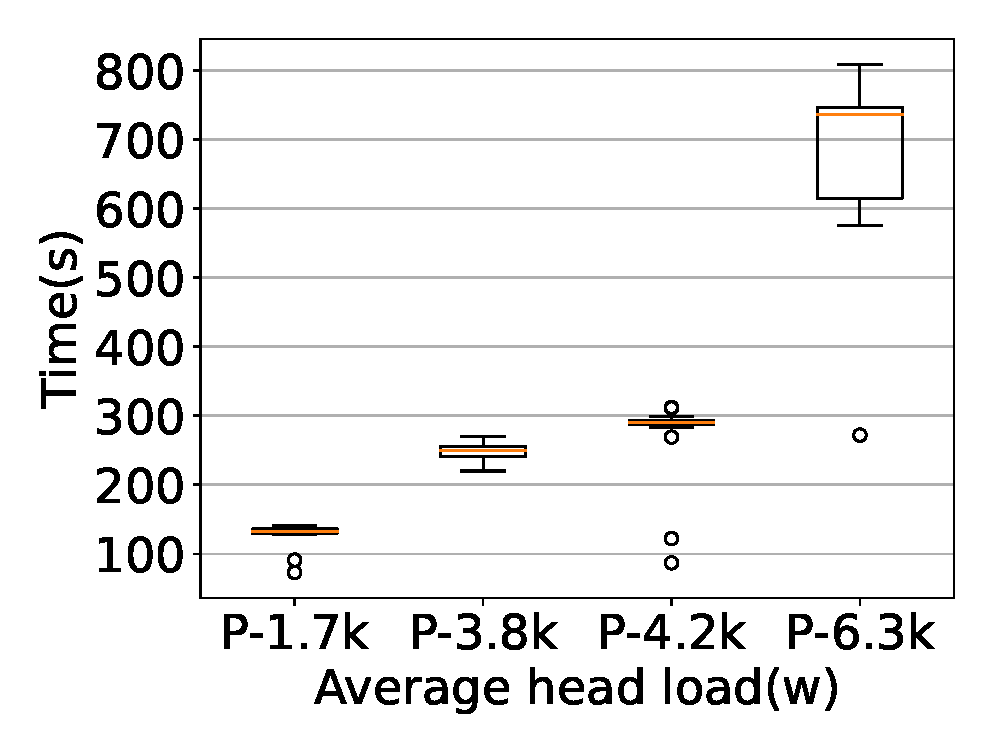
\includegraphics[width=0.45\linewidth]{figures/chapter4/state4.eps}}
\caption{
% The data of the four data sets are generated at different power of the server, which are 1.7kw, 3.8kw, 4.2kw and 6.3kw respectively. Compare the duration time of system on and off   under different power.
在平均负载不同的四个数据集中,阶段\textit{启动}和\textit{关闭}阶段的持续时间分布箱线图
} %图片标题
\label{fig:state}  %图片交叉引用时的标签
\end{figure}
% 与预测某时刻是否要切换到下一阶段这种做法相比,直接预测阶段的持续时间${\tau}_{i}$从而再决定是否切换到下一阶段这种方式更加具有鲁棒性,前者的直接进行阶段切换点预测更容易出现差错,可能会导致过早或过迟地切换到新阶段。
% In comparison to predicting the final time point or classifying whether it is a proper time to switch to next stage, predicting duration time ${\tau}_{i}$ is more robust to give an appropriate stage transformation rather than make accidental faulty predictions or classifications than make accidental faulty predictions or classifications leading to switch to new stage too early or too late.
%The transform rules in Table.~\ref{tab:cooling_dfa} are deterministic and can be easily implemented by programming, so there is no need for manual marking in the phase of generating stage labels.

\begin{table*}[]
\centering
\caption{跳变系统在四种状态下循环,每种状态对应制冷系统的一个阶段}
% \caption{The designed AJ has four circular states and each state is corresponding to one stage in the cooling system.}
\label{tab:cooling_dfa}
\begin{tabular}{llcl}
\toprule
% \multirow{2}{*}{状态} & \multirow{2}{*}{描述}         & \multicolumn{2}{c}{转换规则}                                \\
   状态                  &    描述             & 下一阶段 & 转换触发条件                                   \\ 
   \hline
0-关闭                       & 系统待机                             & 1          & $y_3(t)\geq Ti_{max}$                                \\
1-启动第一阶段                      & 制冷系统启动的第一阶段                     & 2          & $y_1(t)$ 到达某一峰值                            \\
2-启动第二阶段                       & 制冷系统启动的第二阶段 & 3          & \multicolumn{1}{l}{$y_2(t)$ 稳定} \\
3-开机                       & 系统运行                                   & 0          & $y_3(t)\leq Ti_{min}$                                \\
% 4-Shut down                       & system is shutting down                            & 0          & $y_2(t)=0$                                           \\ 
\bottomrule
\end{tabular}
\end{table*}
% \begin{figure}
%     \centering
%     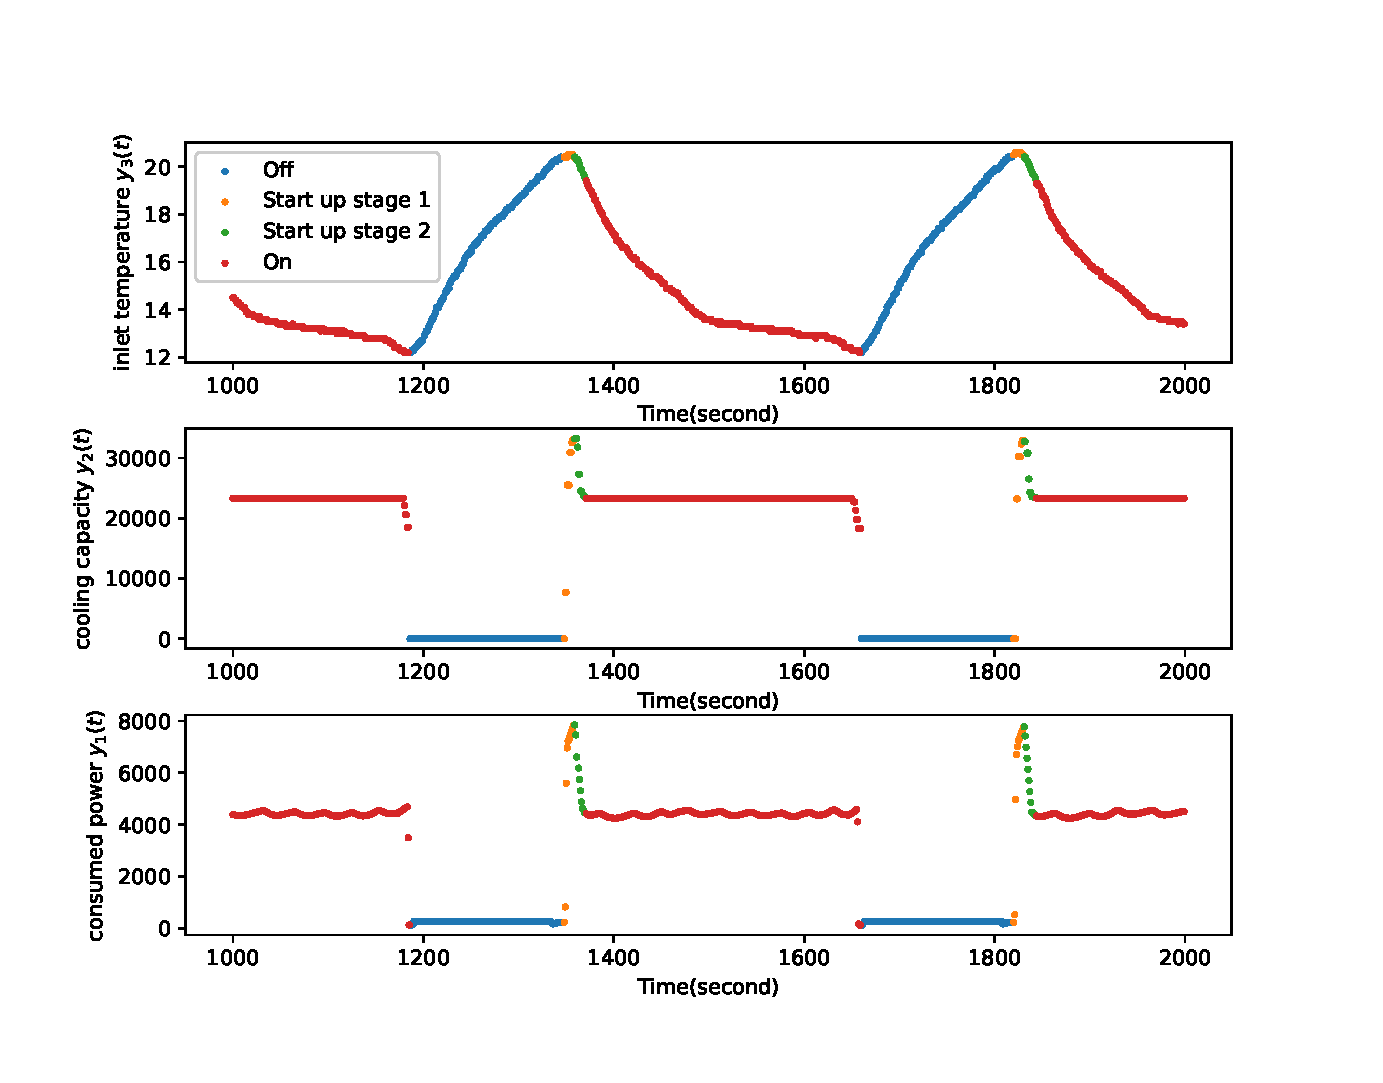
\includegraphics[width=10cm]{figures/chapter4/mark.eps}
%     \caption{Auto Stage labeling result demonstration
%     }
%     \label{fig:stages_mark}
% \end{figure}

% \subsubsection{Multi-stage transformation and duration time prediction}
% According to the prior knowledge, the property of periodic multiple-stage in the system is apparent and we can identify the transform boundaries between adjacent stages from dataset readily.

% The inputs indices include consumed power of the date center $x_1(t)$, room temperature $x_2(t)$. Two inputs variables affect the behaviors of the cooling system and determine three system outputs variables including: instant cooling power $y_1(t)$, cooling production $y_2(t)$, and inlet temperature of cooling system $y_3(t)$.
% Generally, inlet temperature $y_3(t)$ is oscillated periodically in a deterministic range defined by max setpoint $Ti_{max}$ and min setpoint $Ti_{min}$.


% \subsection{Case study 1: Operating Variables Simulation}

\subsection{模型训练}
% \subsection{Model training}
\label{sec:model_training}

我们从Seduce平台采集了四组数据集用于模型的训练与评价,四组数据集均采集于生产运行稳定时段,且运行功率有较大差异,分别为1.7kw,3.8kw,4.2kw,6.3kw。运行功率$x_1(t)$越大,说明当前产热越多。表\ref{tab:sys_in_out_prior}中汇总了各个数据集描述和输入、输出介绍以及序列长度。对于四个数据集,每个数据集中的完整序列长度约为8000-10000,采样时间点为连续非均匀的,平均采样频率约为1条/秒,序列对应的时间长度约为8000s-10000s。
每个数据集的前50\%数据用于模型训练,剩下的数据中,25\%数据用于构建验证集,25\%数据用于模型测试。

对于训练集和验证集,本节使用大小为1600s的滑动窗口对原始序列进行遍历并生成训练样本。
对于每一个训练样本,根据~\ref{sec:notations}定义,前800s为条件范围,用于模型求解预测阶段所需的初始状态,后800s为预测范围,模型预测该范围内的系统输出。
在训练过程中,我们选择在验证集中表现最好的模型用于模型评估。
由于输入的维数较低,且得益于伴随状态法(Adjoint state),训练ODE-net网络对于显存的消耗是极低的。我们选择了较大批大小(batch size=4096)以加速训练。
所有数据集的训练样本被随机排序并分批输入到模型训练。训练过程使用了单块型号为NVIDIA TITAN RTX的并行计算设备(GPU),其显存为24G。
隐状态变量$\boldsymbol h(t)$的大小是20,学习率设置为0.005。

在测试阶段,没有像构造训练集一样对测试集中的完整序列进行分割。序列的前800s被送入编码器模型以生成初始状态,解码器模块在给定序列输入下,以开环的方式预测余下部分的系统输出。预测结果与测试集中的真实输出作对比以评估模型精度。
% During training, the model which performs best in validation dataset will be chosen 
% Owing to low dimensional inputs, we choose a large batch size as 4096 to accelerate training.
% In order to improve the robustness, the training samples of all data sets are randomly ordered and concatenated together before feeding into the model.
% The training phase is executed on a single NVIDIA TITAN RTX with 24G memory.

\begin{figure}[!htbp]
  \centering
  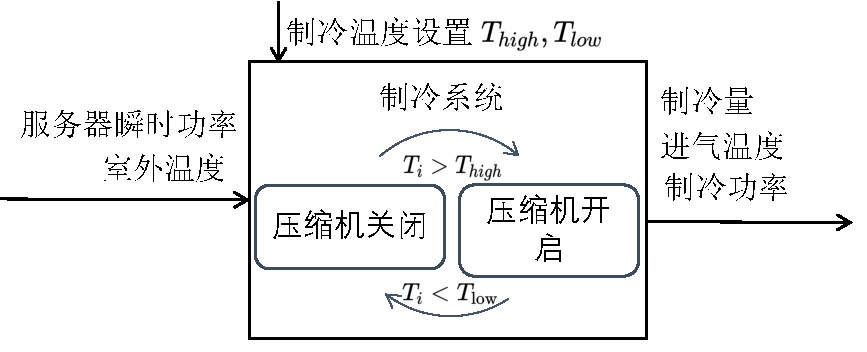
\includegraphics[width=0.8\textwidth]{figures/chapter4/cooling_workloop.pdf}
\caption{制冷系统运行原理概述}
\label{fig:cooling_workloop} 
\end{figure}
%when cooling system is off and slower decrease of inlet temperature when cooling system is working.Together with the stages of cooling system, the consumed power of cooling system $y_1(t)$ and cooling capacity $y_2(t)$ also change periodically with the frequencies and phase positions determined by inputs $x_1(t)$ and $x_2(t)$.  


\begin{table}[ht]
    \centering
\caption{系统输入输出, 不同负载下的数据集和模型的操作}
% \caption{System Inputs-Outputs, data sets based on heat load and model options}
\label{tab:sys_in_out_prior}
\begin{tabular}{cll}
\toprule
\multicolumn{1}{c}{}                                  & 变量定义                      & 描述                                    \\ \hline
\multicolumn{1}{c|}{\multirow{2}{*}{输入}}          & \multicolumn{1}{c|}{$x_1(t)$}& 服务器的瞬时功率,  $W$            \\ \cline{2-3} 
\multicolumn{1}{c|}{}                                 & \multicolumn{1}{c|}{$x_2(t)$}& 环境温度, $^{\circ}C$          \\ \hline
\multicolumn{1}{c|}{\multirow{3}{*}{输出}}         & \multicolumn{1}{c|}{$y_1(t)$}& 制冷系统功率,  $W$                  \\ \cline{2-3} 
\multicolumn{1}{c|}{}                                 & \multicolumn{1}{c|}{$y_2(t)$} & 制冷量,  $W$                     \\ \cline{2-3} 
\multicolumn{1}{c|}{}                                 & \multicolumn{1}{c|}{$y_3(t)$}& 入气口温度,  $^{\circ}C$  \\ \hline
\multicolumn{1}{c|}{\multirow{4}{*}{数据集}} & \multicolumn{2}{l}{"1.7k":服务器稳定运行在1.7kw左右, 长度: 8853s}  \\ \cline{2-3} 
\multicolumn{1}{c|}{}                                 & \multicolumn{2}{l}{"3.8k": 服务器稳定运行在3.8kw左右, 长度: 9771s}  \\ \cline{2-3} 
\multicolumn{1}{c|}{}                                 &
\multicolumn{2}{l}{"4.2k": 服务器稳定运行在4.2kw左右, 长度: 8472s}  \\ \cline{2-3} 
\multicolumn{1}{c|}{}                                 &
\multicolumn{2}{l}{"6.3k": 服务器稳定运行在6.3kw左右, 长度: 8418s} \\ \hline
% \multicolumn{1}{c|}{}                                 &
% \multicolumn{2}{l}{Proportion of dataset for training, validation, and test 5:2:5}  \\ \hline
% Dataset split & training: validation:test = 5:2:5 \\ \hline
\end{tabular}
\end{table}

\subsection{应用研究1: 运行变量仿真}
\label{sec:case-study1}
本节使用基于AJ-ODENet结构的编码器-解码器框架仿真制冷系统的输出。
模型的预测变量为三个:进气口温度,制冷量和制冷机功率。
其中,进气口温度是受制冷系统影响的控制目标变量,表示制冷系统排出的空气温度。制冷量代表制冷系统单位时间产生的制冷量,其直接影响制冷系统中进气口温度的变化~\cite{alonso2020estimating},在压缩机不工作时,制冷量为0。制冷系统开始工作后,制冷量会突然飙升至较高水平。
制冷机功率,表示整个制冷系统瞬时功耗。在制冷系统工作期间功耗较高,待机期间功耗较低。
% In the first place, the framework is used to simulate the operating variables of the concerned cooling system in real time, three typical variables are selected: inlet temperature, cooling production and cooling power. Where, the first variable inlet temperature is an important thermal target of data center affected by cooling production, indicating the air temperature taken by servers. The second one is cooling production generated by compressor, which acts directly on removing heat during the cooling process~\cite{alonso2020estimating},  compressor consumes most of the electricity in the cooling system. And the third estimated variable is cooling power, indicates the instant power consumed by entire cooling system. 
% 另外,系统运行过程中混合稳定和非稳定的两种过程:当系统产生冷空气时,制冷量和系统功耗可以看作是典型的稳定过程(均值和方差相对稳定)。
% 而在此过程中,进气口温度呈指数型下降,则应视为非稳定过程(均值不断下降)。这种稳定性和非稳定性过程混合的系统在工业系统中很常见,
% 所以有必要将多个H-ODE嵌入到AJ-ODEnets模型中。
本节同时引入普通的ODE-Net、ODE-RNN\cite{10.5555/3454287.3454765}、CDE-Net\cite{kidger2020neural}作为本章H-ODENet的对比模型。对比结果如图\ref{fig:models}所示。
% 为了展示H-ODE在多阶段AJ框架中应用的优势,我们对其他可以用来替代H-ODE的模块进行了评估,如嵌入单个ODE模块的结构和嵌入ODE- rnn模块的结构~,并与H-ODE进行了比较,结果如图.~\ref{fig:models}所示。
% In addition, the system operating has a mixture of stationary and non-stationary processes: when the system is producing cold air, energy is consumed stably by compressor, which can be seen as a typical stationary process (with relatively fixed mean and variance). While during this process, the inlet temperature decreases in exponential way, which should be otherwise treated as non-stationary process (the mean keeps dropping). This mixture is commonly seen in industrial systems, and worth the efforts in developing H-ODE network within AJ-ODEnet module (refer to~\ref{sec:dfa-ode-module}).
% In order to demonstrate the advantages of applying H-ODE in multi-stage AJ framework, other options like one Neural ODE structure and ODE-RNN~\cite{10.5555/3454287.3454765} structure as substitutions for H-ODE are evaluated as well to have a comparison, the results are shown in 图.~\ref{fig:models}.
其中图~\ref{fig:models}(a)为真实的系统输出,图~\ref{fig:models}(d)为采用带有H-ODENet的AJ-ODENet模型的预测结果。
在图~\ref{fig:models}(b)中,将AJ-ODEs模块替换为一个单一的稳定型ODENet,此时各阶段的转换不受持续时间预测器控制。此时模型难以对各个阶段间的系统切换边界处给出准确的拟合,尤其是对于持续时间较短的阶段转换位置,如阶段1以及阶段2。在图~\ref{fig:models}(c)中,采用ODE-RNN~\cite{10.5555/3454287.3454765}替换AJ-ODEnets中的混合了稳定性和非稳定性输出的H-ODENet模块。可以发现该结构形成的预测结果难以拟合平滑的输出过程。
相比于其他模型,图~\ref{fig:models}(d)中AJ-ODENet预测的系统输出十分精确,且在阶段转换的边界处能够极好地识别系统输出的剧烈变化。
% Where 图.~\ref{fig:models}(a) is the pattern of original data sets and 图.~\ref{fig:models}(d) is the estimation results by adopting AJ-ODE module with H-ODEnet cells. 
% In 图.~\ref{fig:models}(b), the AJ-ODEs module is replaced by one stationary neural-ODE, in this case, transition of stage is not governed by duration predictor, which could have troubles in precisely fitting dynamics of each stage, especially for the short stage transitions. In 图.~\ref{fig:models}(c) the hybrid stationary and non-stationary 
% H-ODE cells in AJ-ODEnets are replaced by another widely used structure ODE-RNN~\cite{10.5555/3454287.3454765}, which can hardly simulate smooth physical process. 
\begin{figure*}
\centering
\hspace{-0.2in}
\subfigure[Original data]{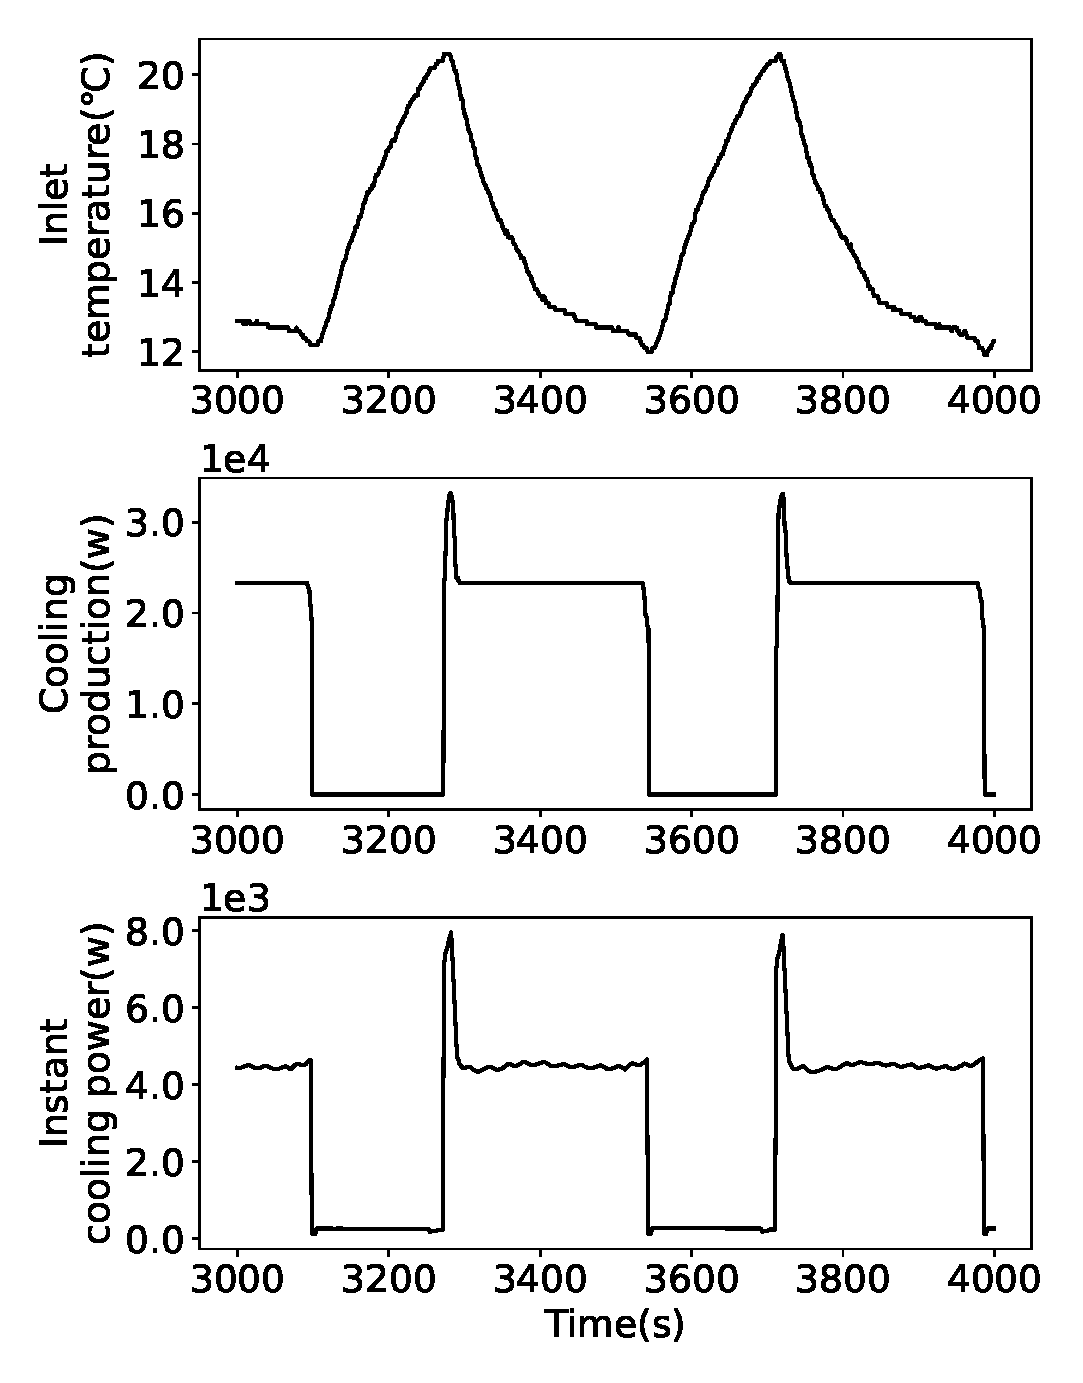
\includegraphics[width=0.45\linewidth]{figures/chapter4/truth.eps}}\hspace{-0.08in}
\subfigure[One Neural ODE]{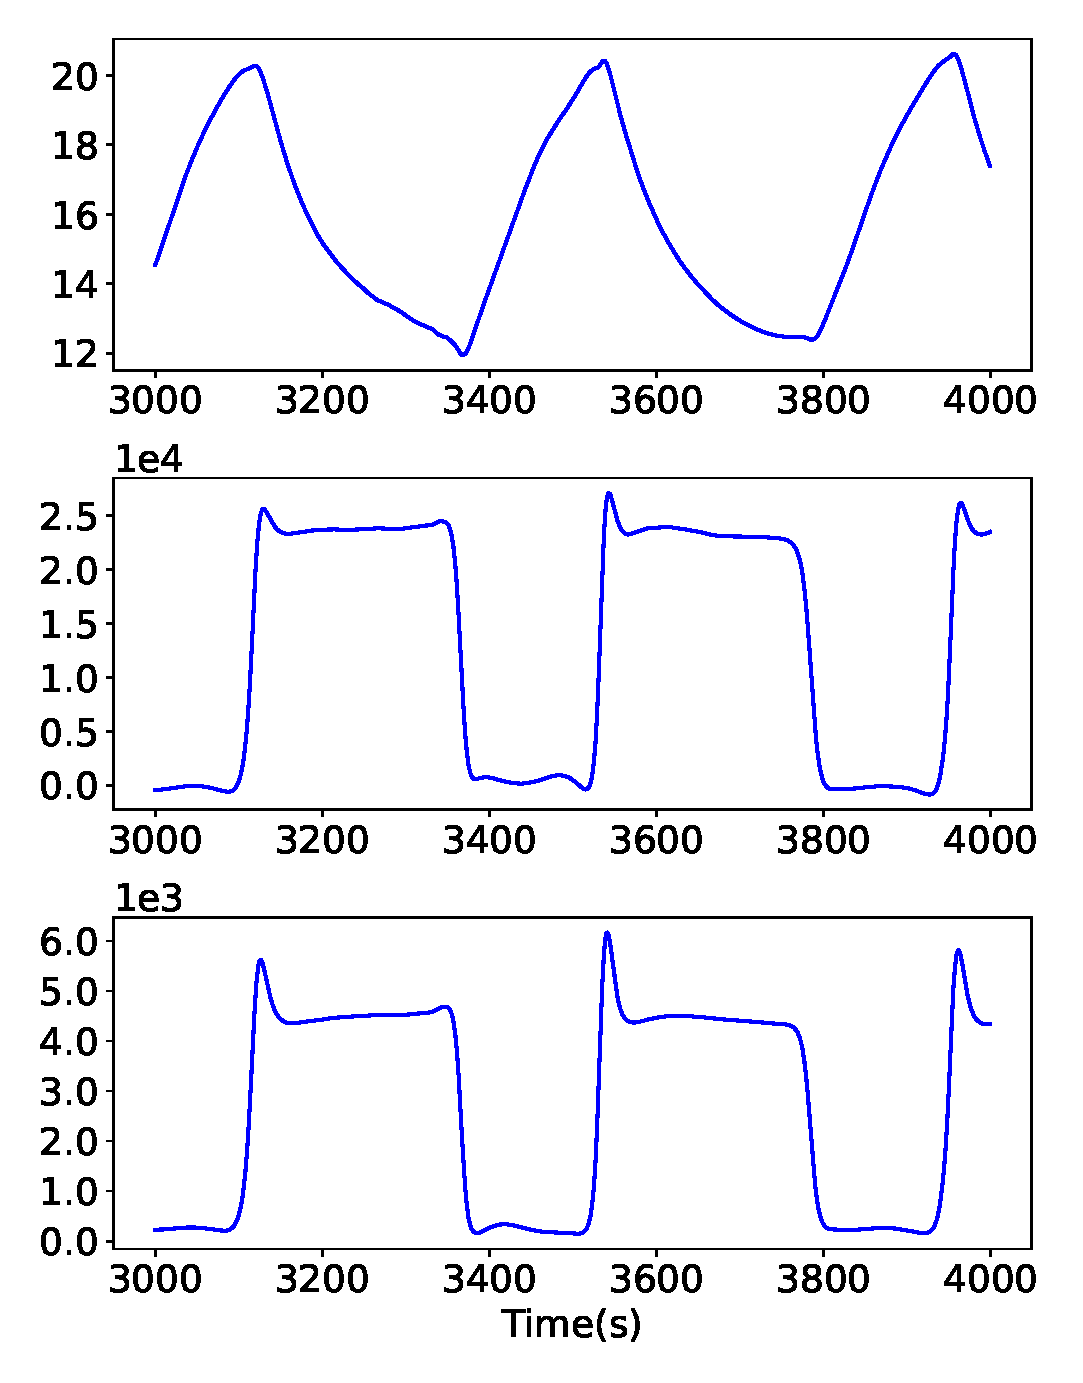
\includegraphics[width=0.45\linewidth]{figures/chapter4/one.eps}}\hspace{-0.08in}
\subfigure[AJ with ODE-RNN cells]{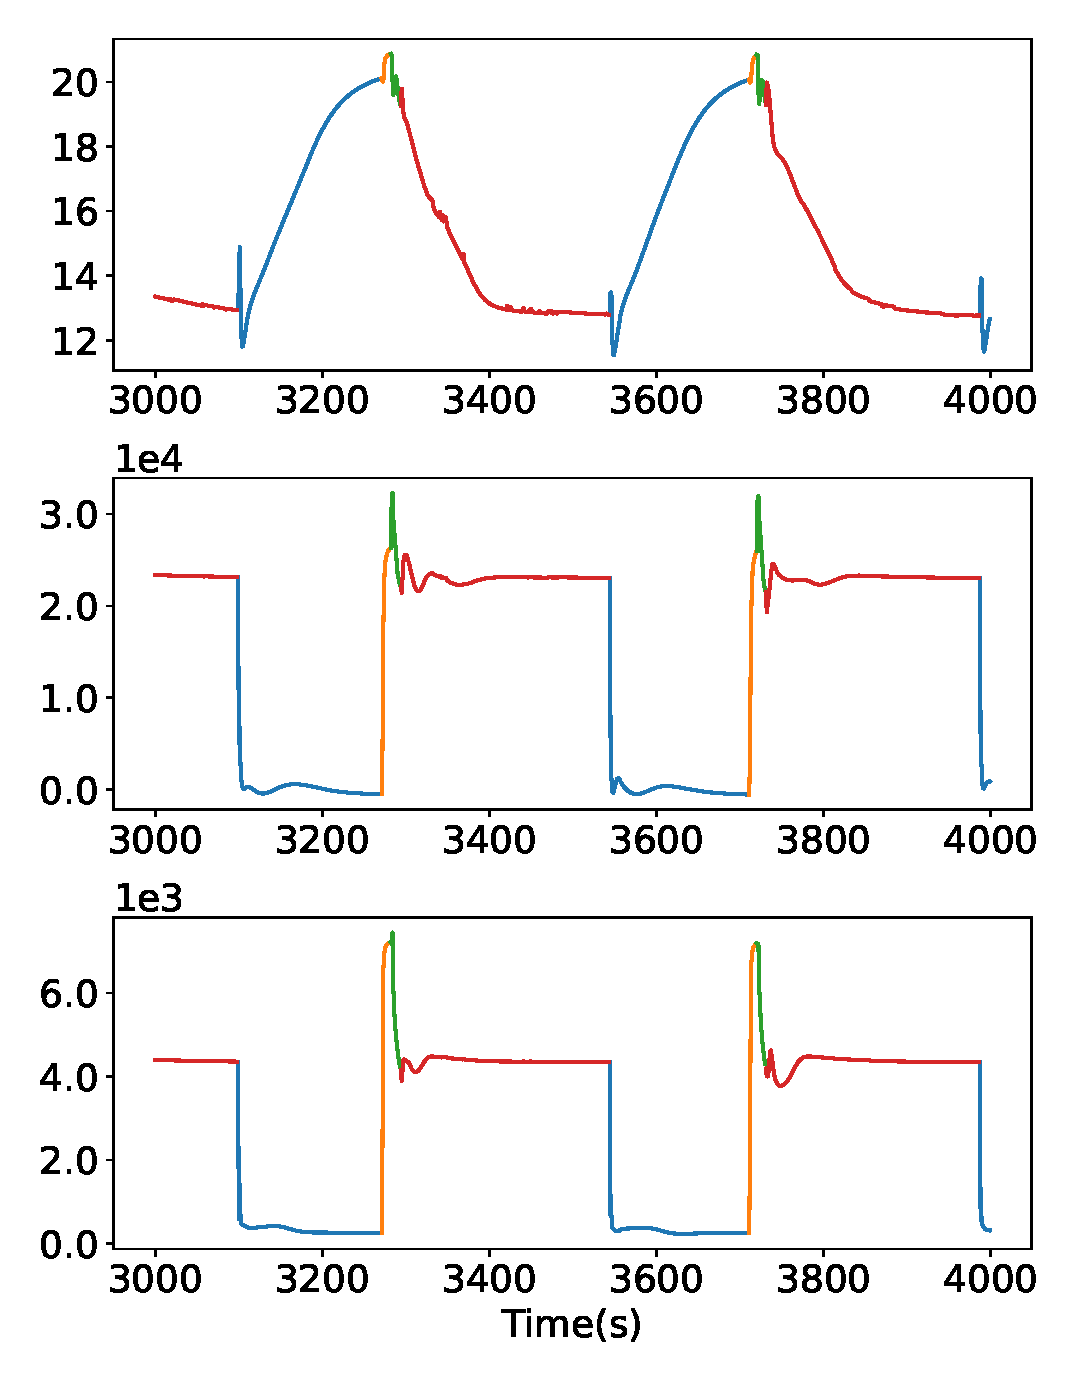
\includegraphics[width=0.45\linewidth]{figures/chapter4/rnn.eps}}\hspace{-0.08in}
\subfigure[AJ with H-ODE cells]{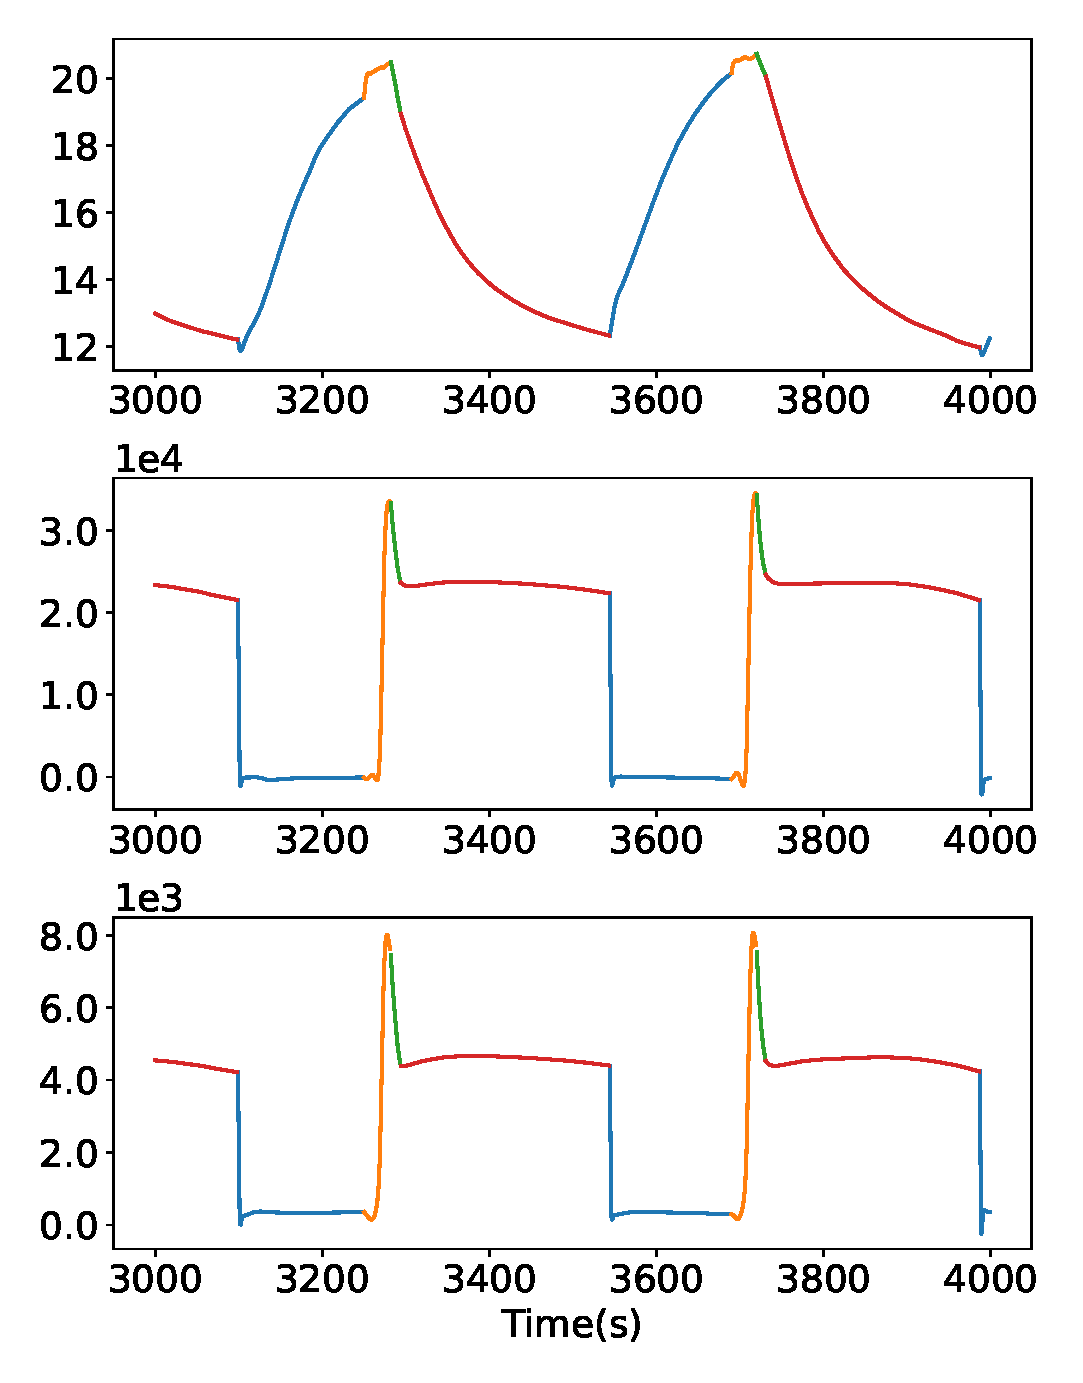
\includegraphics[width=0.45\linewidth]{figures/chapter4/ours.eps}}
\caption{不同模型预测进气口温度,制冷量,制冷机功率的效果对比} %图片标题
\label{fig:models}  %图片交叉引用时的标签
\end{figure*}
% 图.~\ref{fig:}
% \centering
% \hspace{-0.1in}
% \begin{figure}
%     \centering
%     \hspace{-0.1in}
%     \subfigure[The time of state-off]{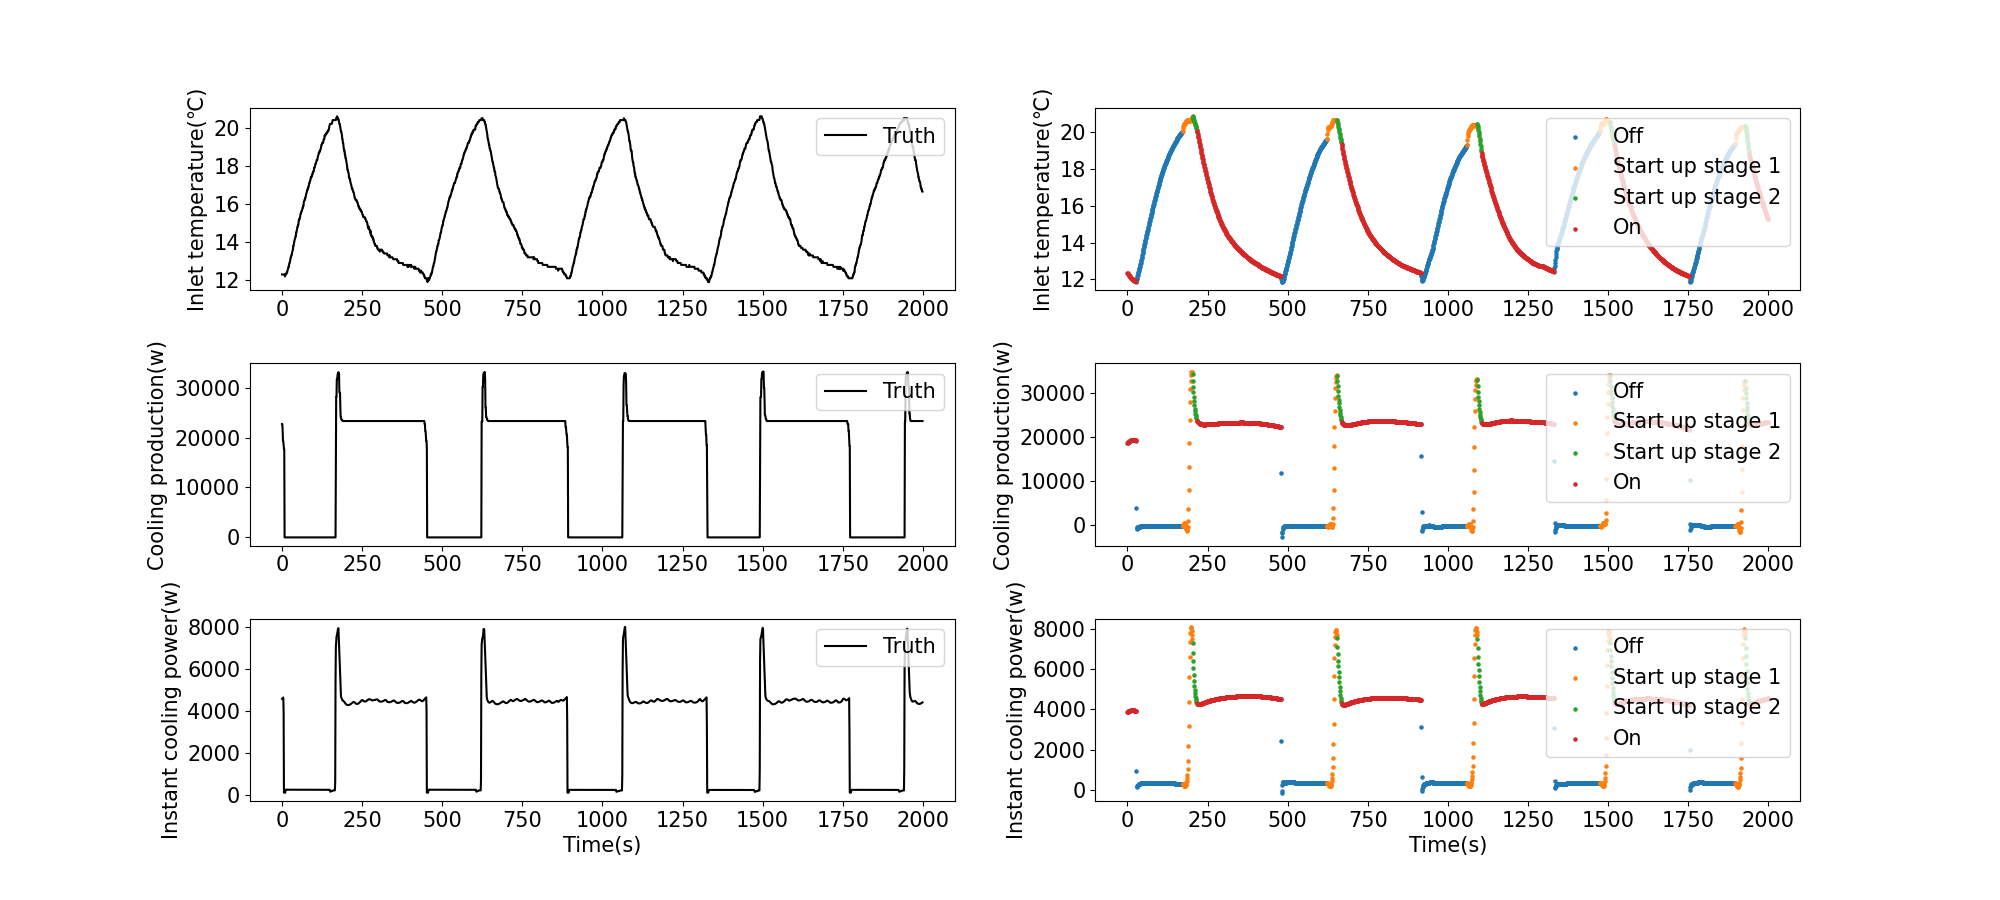
\includegraphics[width=4.7cm]{figures/chapter4/3.8k.png}}\hspace{-0.2in}
%     \subfigure[6.3k]{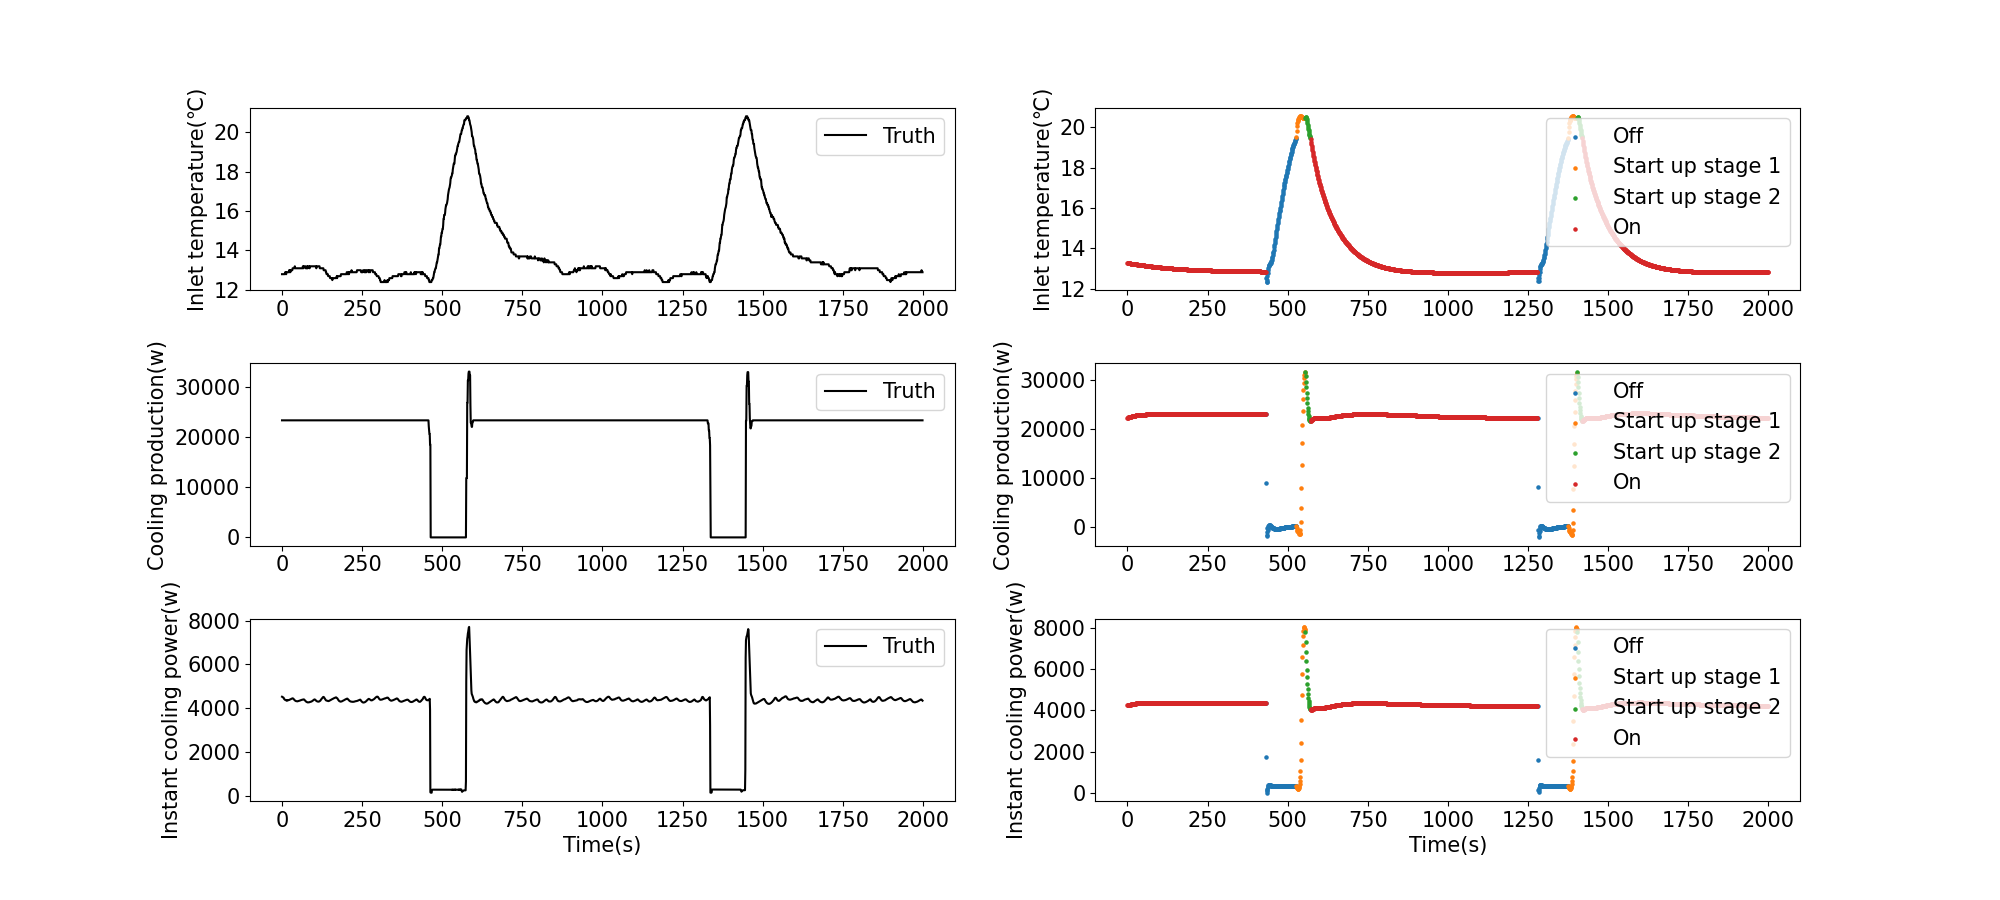
\includegraphics[width=4.7cm]{figures/chapter4/6.3k.png}}
%     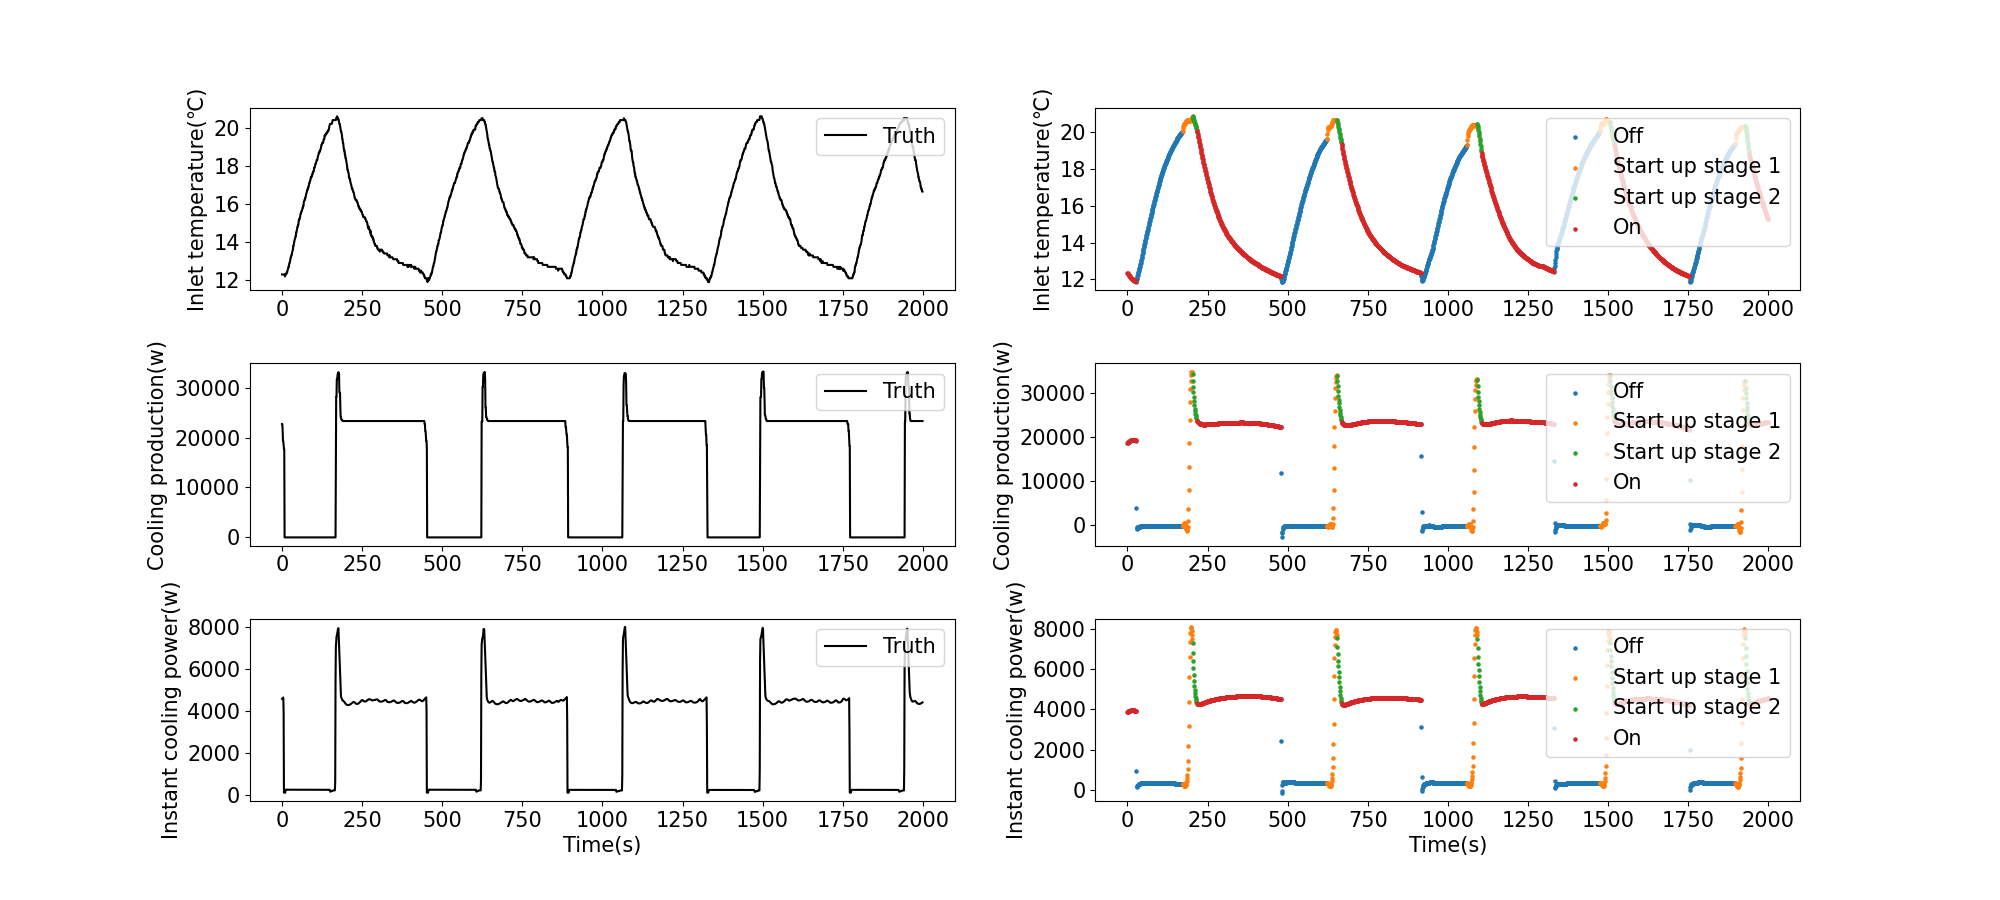
\includegraphics[width=10cm]{figures/chapter4/3.8k.png}
%     \caption{Prediction results of 3.8k-power}
%     \label{fig:3.8k-power}
% \end{figure}
% \begin{figure}
%     \centering
%     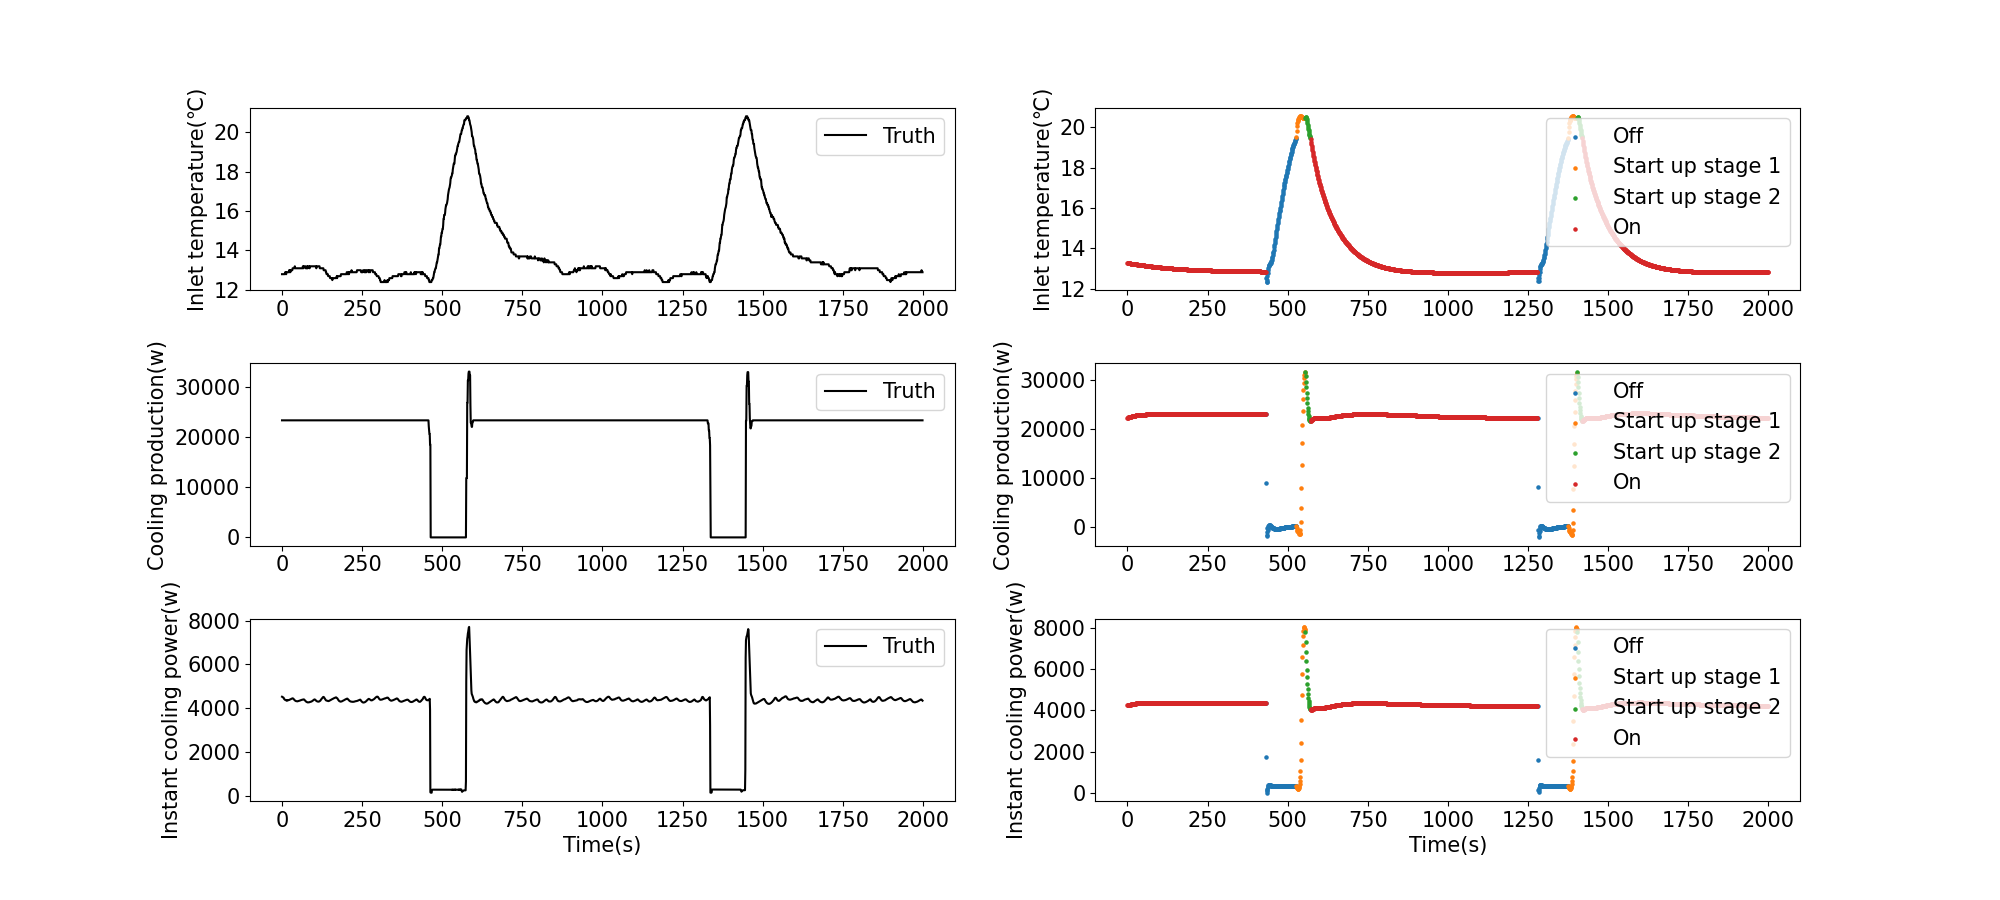
\includegraphics[width=10cm]{figures/chapter4/6.3k.png}
%     \caption{Prediction results of 6.3k-power}
%     \label{fig:6.3k-power}
% \end{figure}
上述实验表明,使用多阶段模型能够将先验知识集成到模型中,相比于单模型结构,能够更好地处理多阶段系统的阶段转换边界预测。
同时结合了非稳定输出和稳定输出的H-ODENet模型能够有效地对系统的多个输出项进行学习,相比于忽视了系统输出时序特性的ODE-RNN模型,能够更准确地预测系统的输出。

% In addition to the predicted accuracy, in using AJ method, the prior knowledge can be integrated into models, to enable advanced studies like the simulation of configuration adjustments, dynamical control and energy consumption optimization. Conversely, for one Neural-ODE or AJ-ODE-RNN structures, it is not applicable.
在预测精度量化方面,由于本文关注于开环预测问题并且需要模型自发地进行阶段切换,伴随着预测范围长度的增加,对于相位的估计误差也将不断累积。
当预测结果中各阶段开始、结束的位置与系统真实输出中阶段的起止位置无法对齐时,此时点对点的误差计算并不适用于量化评估模型的预测误差。
因此,本节对模型预测功耗的长期累积结果进行评估。
对于不同功率的数据集,我们采用训练过的模型预测制冷系统未来在预测范围为$[{t_I:t_{I+L}}]$(共120分钟)下的功耗。
% In terms of the estimation accuracy, given that AJ-ODEnets is applied for open loop estimation and govern the stage transition automatically, the running phases could be affected significantly by the initial point and accumulative error, therefore the point to point accuracy is less meaningful. 
% Accordingly, in order to evaluate the long term simulation capability of the framework, the accumulative energy consumption is estimated over different predictive length, from five minutes to two hours. 
% For the datasets with different power, we employ the trained model to predict the future energy consumption with the predictive range $[{t_I:t_{I+L}}]$ equaling 120 minutes.
% The length of the predicted range ${t_I:t_{I+L}}$ is 120 minutes.
% The predictive error of the accumulative power consumption is evaluated sectionally and measured as Mean Absolute Percentage Error (MAPE).
% By defining the size of the evaluation window as $T$, the prediction error of consumed power, $E(T)$, is measured as:
接下来,依时间尺度对瞬时功耗进行积分可以得到某一时间长度(T)下的累积功耗。
进一步地,可以定义预测功耗的平均绝对百分比误差,$\text{MAPE}(T)$:
% The Mean Absolute Percentage Error (MAPE) of the predicted energy consumption, $\text{MAPE}(T)$, is defined based on the size of the evaluation window $T$:
\vspace{-5pt}
\begin{equation}
\text{MAPE}(T) = \frac{100\%}{n}\sum\limits_{i=1}^{\lfloor\frac{t_{I+L}-t_I}{T}\rfloor}\text{APE}(t_I+T*(i-1),t_I+T*i)
\label{equ:energy_mape}
\end{equation}
其中,其中绝对百分比误差(APE)定义如下:
\begin{equation}
\text{APE}(t_1,t_2) = \left|\frac{\int_{t_1}^{t_2}\hat{y}_1(t)dt-\int_{t_1}^{t_2}y_1(t)dt}{\int_{t_1}^{t_2}y_1(t)dt}\right|
\end{equation}
其中,绝对百分比误差$\text{APE}(t_1,t_2)$衡量了时间范围$[t_1, t_2]$内估计功耗和真实功耗之间的相对误差。图~\ref{fig:mape_evolution}描述了评估窗口的大小T的选取如何影响评估结果 $MAPE(T)$。
可以看出,随着$T$的增加,$\text{MAPE}(T)$ 在开始时剧烈下降,然后缓慢下降。
当评价窗口大小超过35分钟时,所有数据集的MAPE都趋于稳定,说明此时真实系统输出序列与预测序列之间的阶段起止位置相位差对于评估长期功耗的预测精度不再产生影响。
因为本节对比了$T=30$分钟下,不同模型对于累积功耗预测结果的MAPE,结果如表~\ref{tab:Compare power}所示。
结果表明对于所有数据集,AJ-ODENet预测结果的MAPE稳定低于5\%,优于其他三个对比模型。
充分证明了本文提出的AJ-ODENet框架能够以开环预测的方式在长时间尺度下精确地仿真制冷系统的累积功耗。

从计算复杂性的角度,本节对四个模型在测试集单批数据上执行\eqref{equa:initial_state}以及\eqref{equ:decoding}两个过程的时间消耗进行了对比。
Neural ODE作为耗时最短的模型,将其时间消耗作为基准。其他模型的推理时间均处以该基准以得到相对尺度下的时间对比结果。
Neural ODE的相对时间消耗为1.0。对比结果如表\ref{tab:Compare power}的最后一列所示。
相对时间尺度下的对比结果表明引入阶段转换预测器会增加计算的开销,该时间消耗主要用于更新阶段变量及阶段持续时间。

% % The Mean Absolute Percentage Error (MAPE, see 式~\ref{equa:mape}) has been calculated between real and estimated energy consumption in the test datasets. We select a series with a time duration of 120min, In order to calculate the power consumption of different duration $t_r$, from 5 minututes to 120 minututes.According to the formula $ n=120/tr$, get n sample points. 
% % Where, $n$ is the number of sample points, $\hat{e}_i$ is the estimated value and $e_i$ is the real value.  
% % As illustrated by 式~\ref{equa:energy},  where the value $a$ is the beginning of this sequence time, the value $b$ is the ending, and $y_1(t)$ is the instantaneous consumed power of the cooling  system. 
% % The energy consumption is calculated through the integral of power over a period of time. 
% where absolute percentage error(APE) measures the relative error of the estimated energy consumption, which is calculated through the integral of power over a period of time $[t_1, t_2]$. 
% 图.~\ref{fig:mape_evolution} describes how does the size of evaluation window affect the evaluated results $E(T)$.
% % The 图.~\ref{fig:mape_evolution} shows the MAPE of the energy consumption estimation results over prediction duration. 
% It can be seen that, with the increase of $T$, $\text{MAPE}(T)$ declines dramatically at the beginning then becomes smaller and smaller. 
% When the size of evaluation window exceeds 35 minutes, the MAPE of all datasets are stably below 5\%, the phase difference will have little impact on estimating long-term energy consumption. 
% Tab.~\ref{tab:Compare power} also compares the MAPE of predicted energy consumption from proposed AJ-ODEnet with the results from the other competitors.
% The results indicate that, in terms of the open loop estimation, the proposed framework can eliminate the impact of initial point and obtain satisfying accuracy for energy consumption simulation with a predictive range longer than half an hour. 
\begin{table}[t]
    \centering
    \caption{
    % of H-ODEnet and 
    % Power estimation error comparison between One-ODE and H-ODE ,The total length of each test set is 120 minutes. Select the sequence every 30 minutes, calculate the power consumption of the truth value and the predicted value, and then calculate the MAPE. Truth power consumption$P_{truth}=(p_1,p_2,p_3,p_4)$,Predicted power consumption$P_{pred}=(\hat{p_1},\hat{p_2},\hat{p_3},\hat{p_4})$
    The comparison of energy consumption prediction and the relative computational efficiency}
    \resizebox{\linewidth}{!}{
    \begin{tabular}{lccccc} 
    \toprule
                                & \multicolumn{4}{l}{\textbf{\textbf{Average heat load of dataset}}} & \multirow{2}{*}{\begin{tabular}[c]{@{}c@{}}Relative \\Time\end{tabular}}  \\
    \multicolumn{1}{c}{}        & 1.7k          & 3.8k          & 4.2k          & 6.3k               &                                                                           \\ 
    \hline
    AJ-ODENet(ours) & \textbf{4.20} & \textbf{1.51} & \textbf{3.46} & \textbf{2.53}      & 3.2                                                                        \\
    One Neural ODE              & 6.18          & 19.99         & 6.24          & 3.39               & 1.0                                                                         \\
    Jump with CDE\cite{kidger2020neural} cells         & 8.25         & 2.73          & 6.62         & 3.87              & 3.8                                                                        \\
    Jump with ODE-RNN cells     & 38.26         & 9.94          & 10.58         & 31.90              & 3.4                                                                        \\
    \bottomrule
    \end{tabular}}
    \label{tab:Compare power}
    \vspace{-15pt}
    \end{table}

% \begin{equation}
% \label{equa:mape}
%     MAPE=\frac{100\%}{n}\sum\limits_{i=1}^{n}|\frac{\hat{e_i}-{e_i}}{e_i}|
% \end{equation}


% \begin{equation}
% \label{equa:energy}
%     Energy = \int_{a}^{b}y_1(t)dt
% \end{equation}

% \begin{equation}
% \label{equa:energy}
%     n = 2/x
% \end{equation}

\begin{figure}
    \centering
    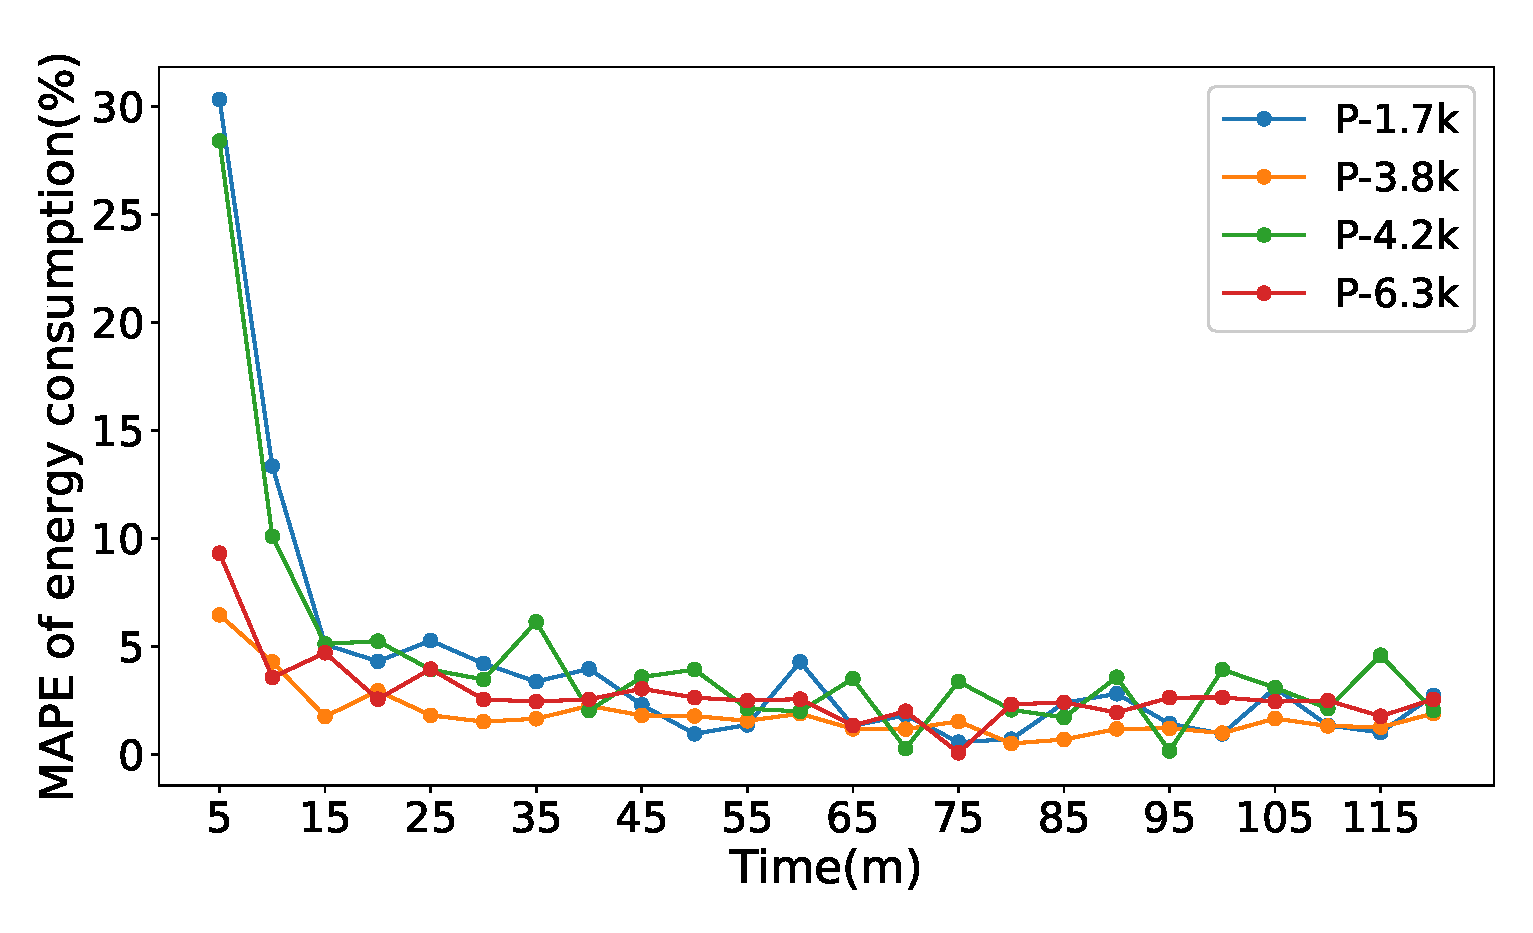
\includegraphics[width=0.8\linewidth]{figures/chapter4/power_error.eps}
    \caption{预测不同时间长度的功耗的MAPE的变化}
    \label{fig:mape_evolution}
\end{figure}

%Relative error of predicted power consumption at different intervals,According to the instant cooling power sequence value predicted by AJ-ODEnets, calculate the power consumption of the system over a period of time, compare it with the real power consumption value, and calculate the error.  Compare the power consumption error between the real value and the predicted value for different duration time (5min, 10min... 120min)


%Compare the prediction effects of different models. 图.re a is the truth sequential data, figure B is the prediction result of one stable ODE model, figure C is the experimental effect of Ode RNN, and figure D is the result of our model

\subsection{应用研究2: 制冷系统进气口温度设定点优化}
\label{sub:case-study2}
进气口温度设定点是影响制冷系统运行的关键设置参数之一。
通常,系统要设定通入进气口的空气温度阈值(上限$Ti_{max}$和下限$Ti_{min}$),以保证运行环境的安全。
通常,对于大部分的制冷系统,初始的进气口温度设定点是固定的,配置值低于ASHRAE TC9.9~\cite{ashraeTC992011}(数据中心电源设备热指南和最佳实践)中定义的标准,没有充分考虑实际的制冷需求。
以本章研究的制冷系统为例,其温度阈值为$12^\circ C$,$20\circ C$。
数据集中进气温度在两个阈值之间周期性变化。

出于提高能源效率和确保生产过程安全的目的,本节保持温度上限值不变,只调整下限值以减少能源消耗。
然而,要确定最佳温度阈值是很棘手的。
如果阈值设置得太低,由于过度冷却会浪费大量电能。
如果阈值设置得太高,压缩机的制冷重启过程将更加频繁,这将在单位时间内形成更多的峰值功率。从图~\ref{fig:orginal}中可以看出,制冷系统重新启动时的功耗显著高于提供稳定冷却时的功耗。
因此,盲目地增加温度下阈值反而可能会导致的整体的能耗增加。
% 实际上,最佳温度设定点随热负载的不同而变化,尤其是温度下限。如果下限设置过低,会因过度制冷过多而浪费电能;过高会导致压缩机频繁停机和启动,如图1所示(见表~\ref{tab:cooling_dfa}),在阶段一启动时功率峰值会很高,这些峰值过多会浪费额外的电能,。

在本节实验中,我们试图寻找最佳的温度下限以达到更好的能源效率。形式化地,寻找最佳温度下限$Ti_{min}^{*}$可以表示为一个单目标优化问题,考虑到以下因素:热负载、环境温度、进气口温度的上下限:
\begin{equation}
    \begin{aligned}
       Ti^*_{\min}&=\mathop{\arg\min}\limits_{Ti_{\min}} \int_{0}^{T} \hat{y}_{1}(t) dt \\
       &\text{ Where } \hat{\boldsymbol{Y}}_{0: T}=F\left(\boldsymbol{X}_{0: T},Ti_{\min}, Ti_{\max},\boldsymbol{\zeta}\right)
    \end{aligned}
    \label{equ:optimazition}
    \end{equation}
其中$\hat{\boldsymbol{Y}}_{0: T}$和$\hat{y}_{1}(t)$分别表示模型预测的系统输出和模拟的瞬时功耗。
在给定系统输入和恒定的上限值的条件下,其优化变量是温度下限的设定点,优化目标是最小化累计能耗。
式\eqref{equ:optimazition}中的$\boldsymbol{X}_{0: T}$为测试数据集中的系统输入,其中包括所有时刻的热负载以及环境温度。
式\eqref{equ:optimazition}中的$F(\cdot)$表示在给定输入和温度阈值$Ti_{max}$和$Ti_{min}$下,预测制冷系统的输出。
% The inlet temperature set points are one of the key configurations of cooling systems. Generally, they put the temperature variation thresholds (upper and lower boundaries) for the air temperature to the front of the servers, to guarantee the ambient and secure operating environment. 
% Normally, for the workplace like Data Centers, the initial set points are fixed and configured far below the standards defined by ASHRAE TC9.9~\cite{ashraeTC992011} (Data Center Power Equipment Thermal Guidelines and Best Practices), without considering the actual cooling requirement. 
% Actually, optimal temperature set points vary with the heat load, especially for the lower boundary: if it is set too low, energy will be wasted due to over cooling; if too high, compressor may suffer from frequent stop and restart, additional energy can be wasted due to too many power peak as seen in stage 1 (refers to Tab.~\ref{tab:cooling_dfa}). 

本节中,我们利用上一节~\ref{sec:case-study1}中训练的编码器-解码器AJ-ODEnets模型,
在给定不同下边界温度设定点的情况下,仿真系统能耗以及温度变化,同时评估特定时间区间内的累积制冷功耗。
实验采用\secref{sec:case-study1}中所述的三个数据集,其的平均负载分别为1.7k、3.8k和6.3k。
温度下阈值设置点从$12^{\circ}C$逐渐增加到$18^{\circ}C$,调整间隔为$0.5^{\circ}C$ 。
% In order to simulate the cooling system with different $Ti_{\min}$, the prediction in $F(\cdot)$ is slightly different from the trained model $f(\cdot)$.
为了模拟不同$Ti_{min}$下的冷却系统运行过程,$F(\cdot)$中的预测过程与原始训练模型$f(\cdot)$略有不同。
% In particular, the sojourn time predictor in stage \textit{On} is replaced by a specific transformation rule.
特别地,在阶段\textit{On}下的持续时间预测器被特定的转换规则所替代。
% Just as the rule in Table~\ref{tab:cooling_dfa}), the stage immediately transitions from 3 (\textit{On}) to 0 (\textit{Off}) if the inlet temperature is cooled down to $Ti_{\min}$. 
如表~\ref{tab:cooling_dfa}中的规则,如果进气口温度经过冷却下降到$Ti_{min}$,预测模型立即将阶段变量从3(\textit{On})过渡到0(\textit{Off})。

    % The stage transition predictor in the proposed model is designed based on sojourn time prediction,  nevertheless, the rules could also be set manually in order to meet simulation requests.
    尽管本章所提出模型中的阶段转换预测器是基于持续时间预测器设计的,为了满足不同制冷系统运行参数的仿真需要,也可以手动设置状态转换规则。
    虽然在上述模拟过程中的温度下限与训练数据集对应的阈值参数是不同的,但AJ-ODENet仍然支持手动调整阶段过渡阈值以支持此类外推预测。
    % Although the lower temperature threshold in simulations is out of the range of the training dataset, AJ-ODENet can still support extrapolation by adjusting manually stage transition thresholds.
    相比于没有引入系统先验的稳态模型~\cite{Yilmaz2007},基于先验知识的模型更具可解释性和可扩展性。
    % Compared with the steady state model~\cite{Yilmaz2007}, the prior knowledge-informed model is more interpretable and extensible.
    % Meanwhile, in order to model the variation of inlet temperature as a non-stationary process, the temperature is made to climb steadily during stage \textit{Off} and decreased steadily during stage \textit{On}.
    同时,本章将进气口温度的变化建模成非平稳过程,使得在阶段\textit{Off}期间,进气温度会稳定地上升,在阶段\textit{On}期间,温度会稳定地下降,进而确保温度必然能够触达给定的阈值,
    % This property is consistent with the prior knowledge of the system and is necessary to guarantee that the inlet temperature will continue to vary until reach the wanted thresholds.
    这一模型特性与系统的先验知识一致,是保证进气口温度能够持续变化直至达到阈值的必要条件,有效避免了模型无限期停留某一阶段内难以跳出的情况。

% 在下边界温度设定点不同的情况进行系统仿真实验中,我们对于从\textit{On}阶段到\textit{Off}阶段的转换过程,用了一个转换规则替换了持续时间预测器。
% 如表~\ref{tab:cooling_dfa}所示的系统先验知识,随着制冷系统温度降低,当前进气口温度小于$Ti_{min}$时,系统将切换到阶段 \textit{Off},
图~\ref{fig:lowerbound_simulation}显示了对于热负载约为3.8k的数据集, 不同的进气口温度下限对制冷系统的影响。
仿真时间为1000秒。随着温度下限设置点从$12^{\circ}C$增加到$18^{\circ}C$,在相同的持续时间内,稳定制冷阶段的时间不断缩减。与此同时,1000秒内包含了更多的制冷系统启停周期。这导致系统的主要功耗来自于由\textit{Off}阶段转变为\textit{on}阶段的系统启动功耗,而非制冷功耗。

% In order to find the optimal lower boundary temperature set points under different heat loads. 
% we make use of the Encoder-Decoder AJ-ODEnet model built in the first case study~\ref{sec:case-study1}, and run simulations by calculating the energy consumption within same duration under different lower temperature set point for three datasets.
% % as they represent for different heat loads (higher IT loads will generate more heat). 
% The three datasets represent for different average heat loads (higher IT loads will generate more heat) including 1.7k, 3.8k, and 6.3k.
% In each simulation with specific lower boundary temperature $Ti_{min}$, we substituted the duration predictor with a rule in the transformation from \textit{On} stage to \textit{Off} stage.
% With the cooling system brings the temperature down, the system will switch to the stage \textit{Off} when the current inlet temperature is smaller than $Ti_{min}$, as like the system prior knowledge shown in Tab.~\ref{tab:cooling_dfa}.
% % The set points can be modified in Stage Transition Predictor (refers to Sec.~\ref{sec:stage_trans_predic}), where the configurations are integrated as system prior knowledge. 
% 图.~\ref{fig:lowerbound_simulation} illustrates the impact of different lower boundaries on the behaviors of cooling system (dataset 3.8k), with the set point increasing from $12^{\circ}C$ to $18^{\circ}C$, more loops are included within same duration.
% The main stages which consume the energy most change from \textit{On} stage to \textit{start up 1} and \textit{start up 2} stage.
\begin{figure*}[h]
\centering
\subfigure[$12^{\circ}C$]{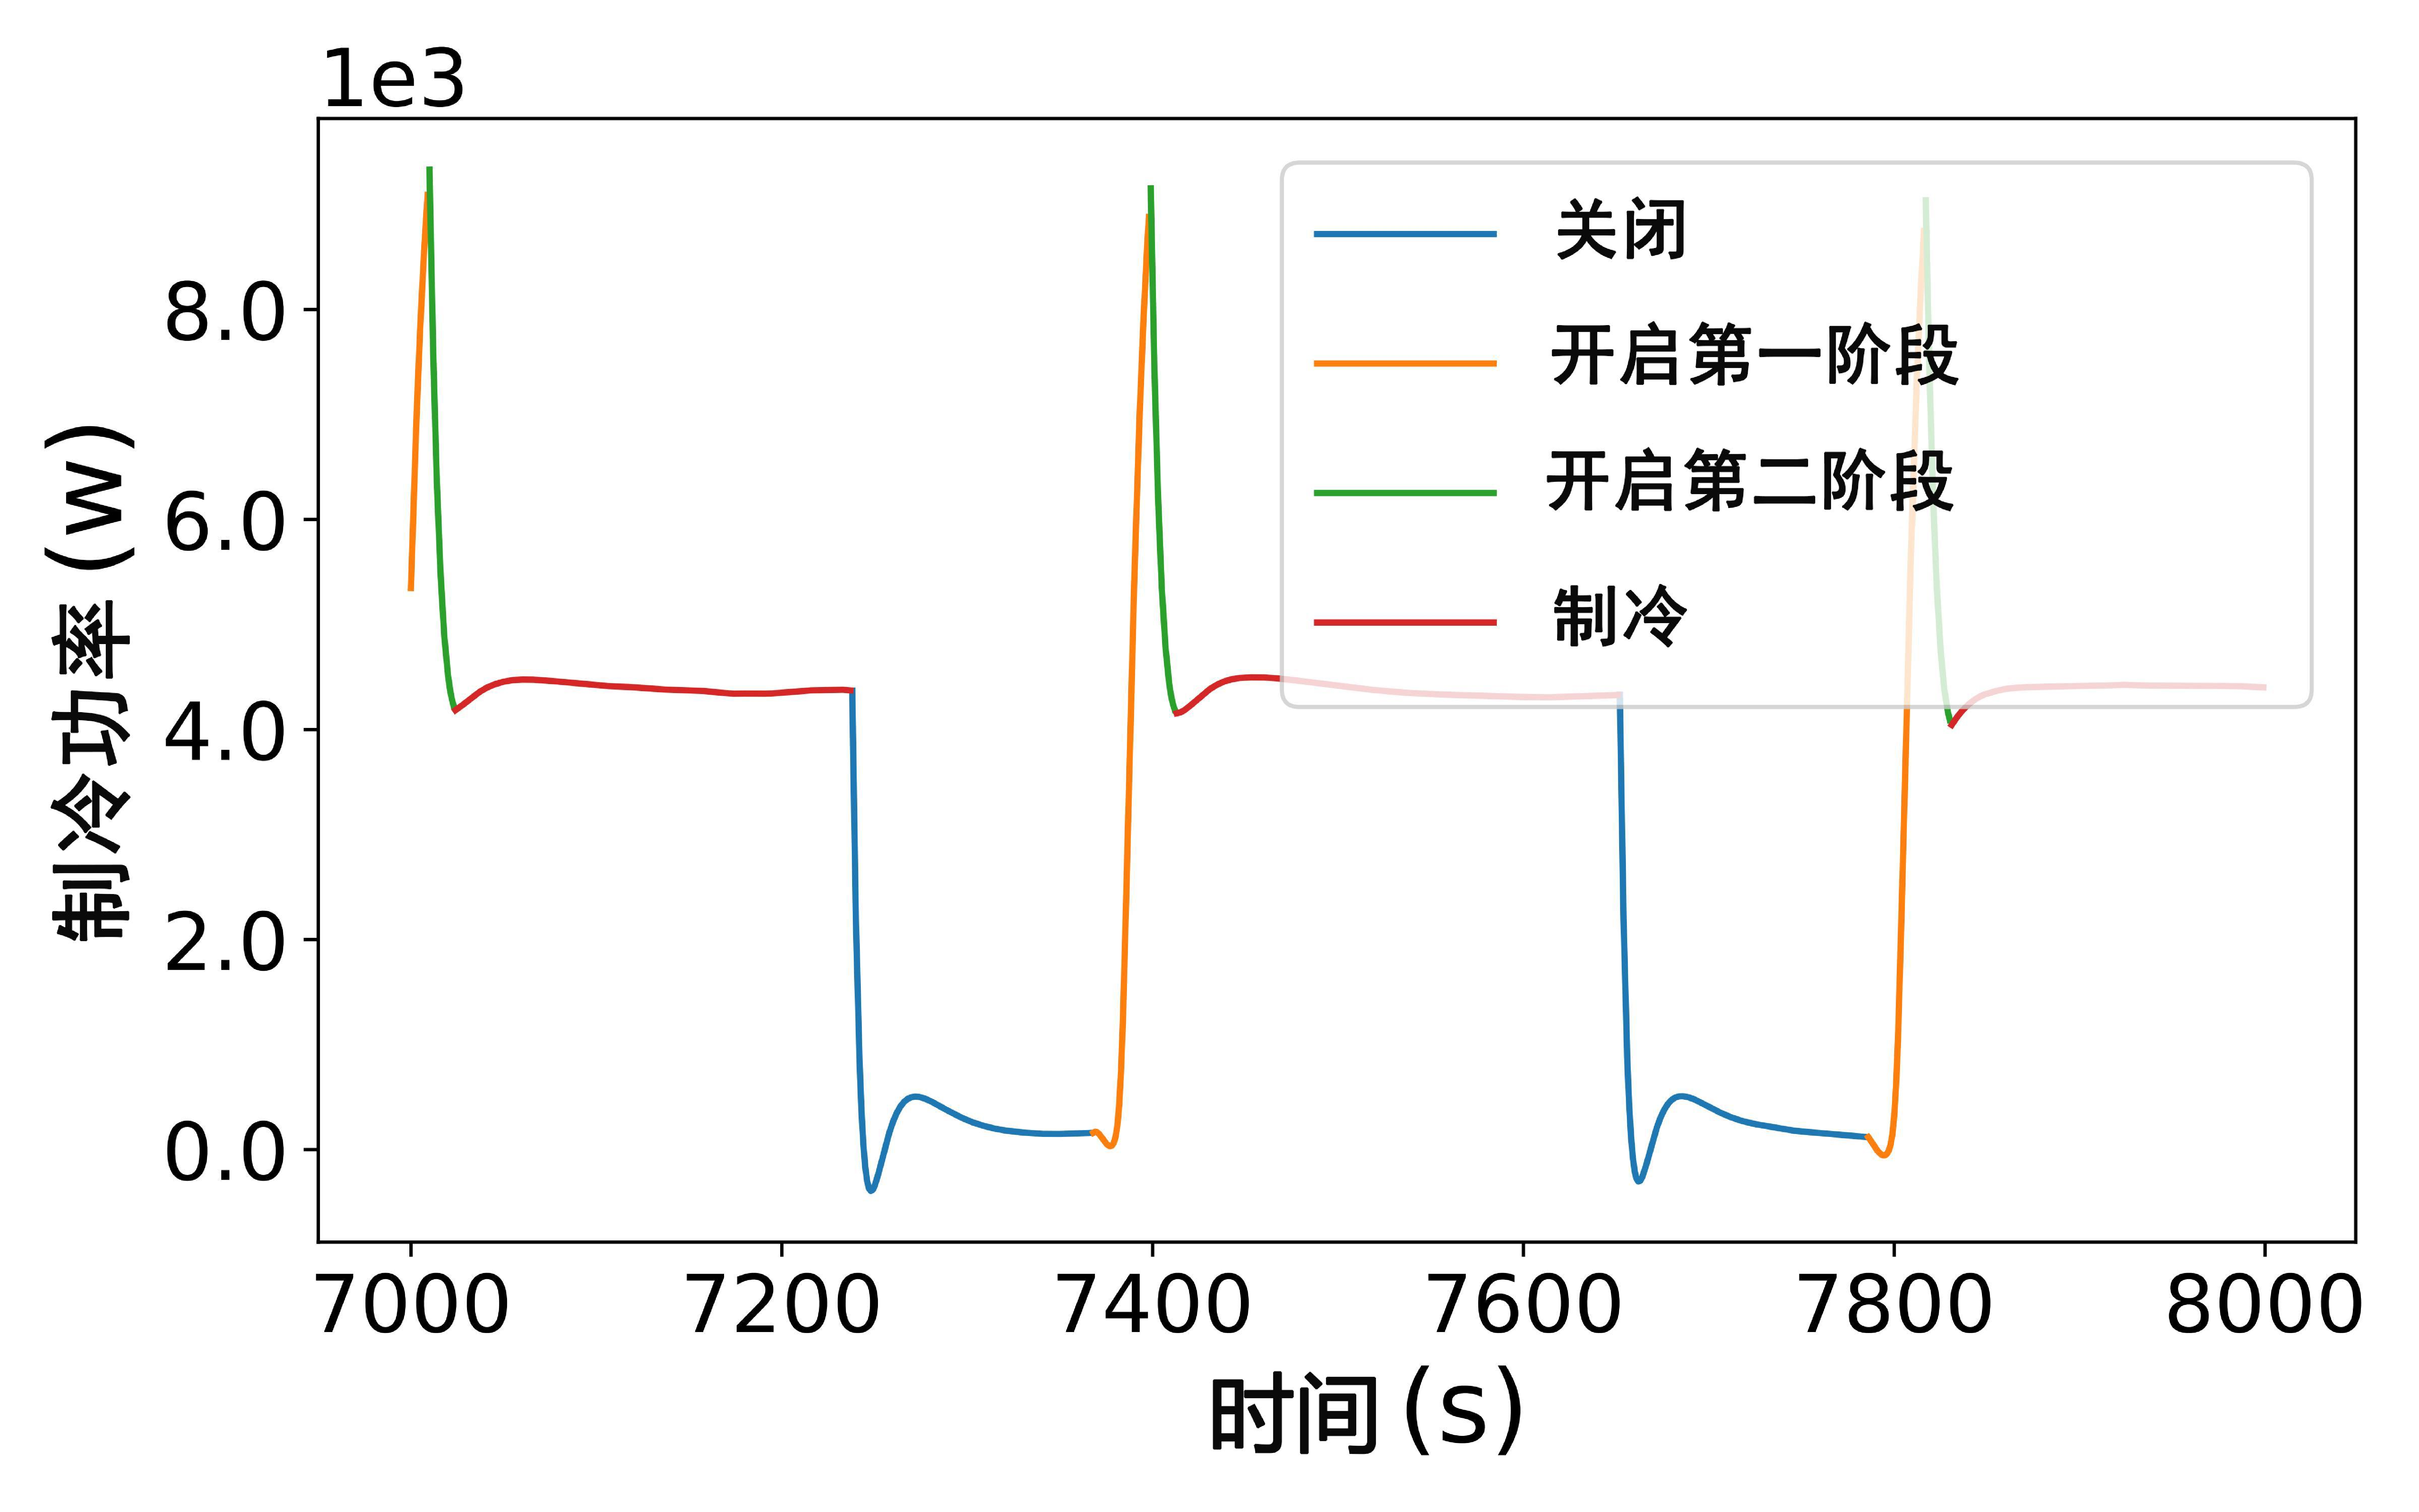
\includegraphics[width=0.45\linewidth]{figures/chapter4/12.pdf}} \hspace{-0.1in}
\subfigure[$14^{\circ}C$]{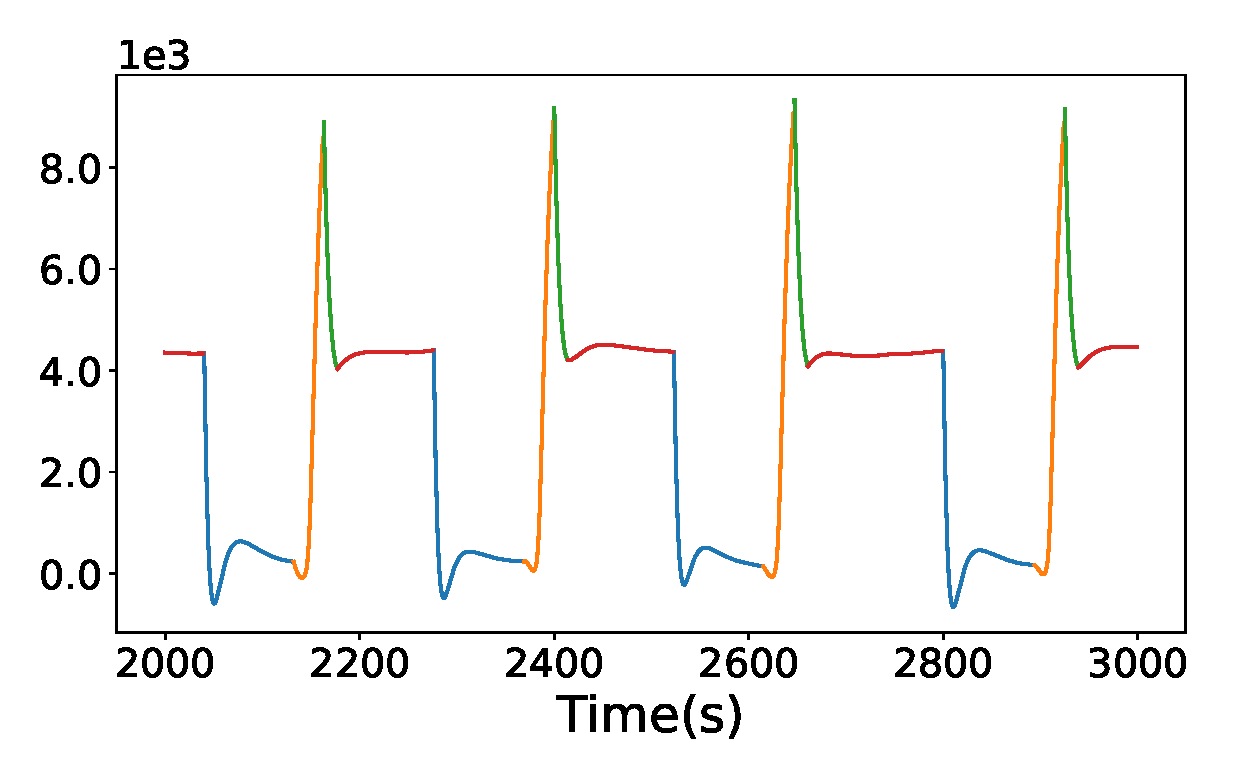
\includegraphics[width=0.45\linewidth]{figures/chapter4/14.eps}} \hspace{-0.1in}\\
\subfigure[$16^{\circ}C$]{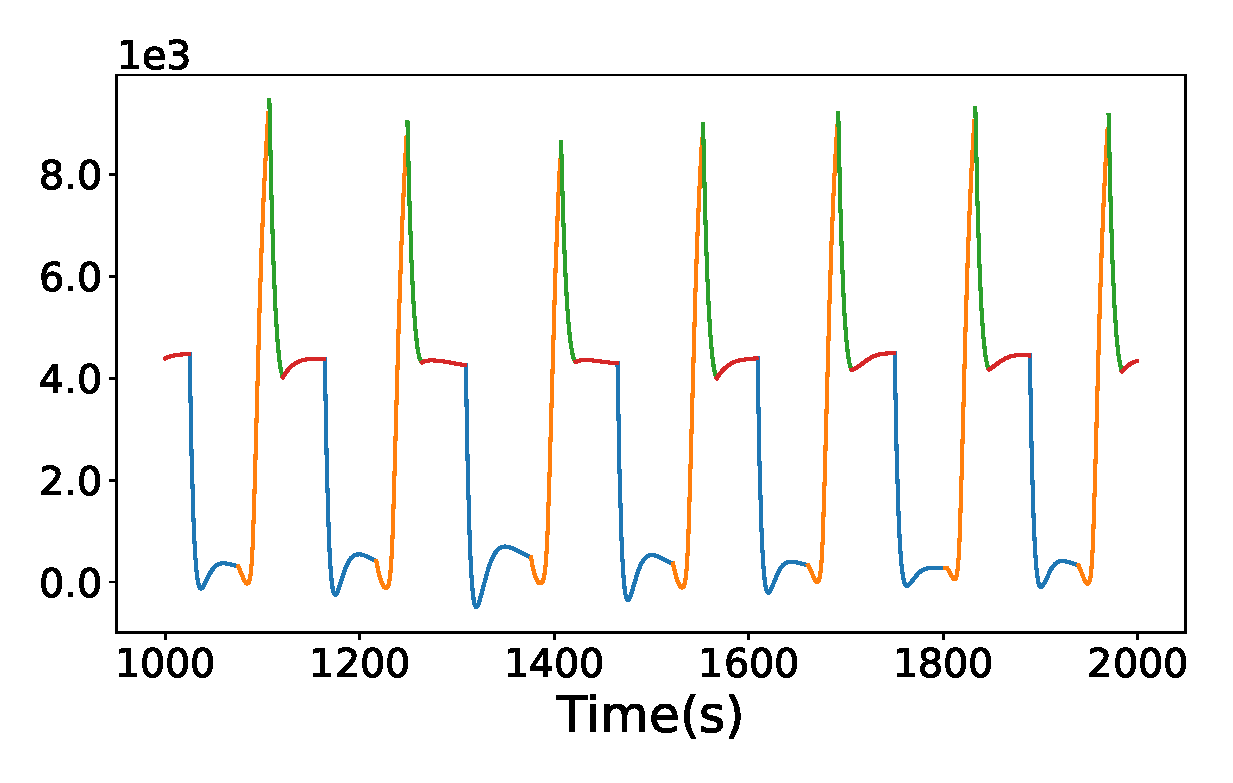
\includegraphics[width=0.45\linewidth]{figures/chapter4/16.eps}} \hspace{-0.1in}
\subfigure[$18^{\circ}C$]{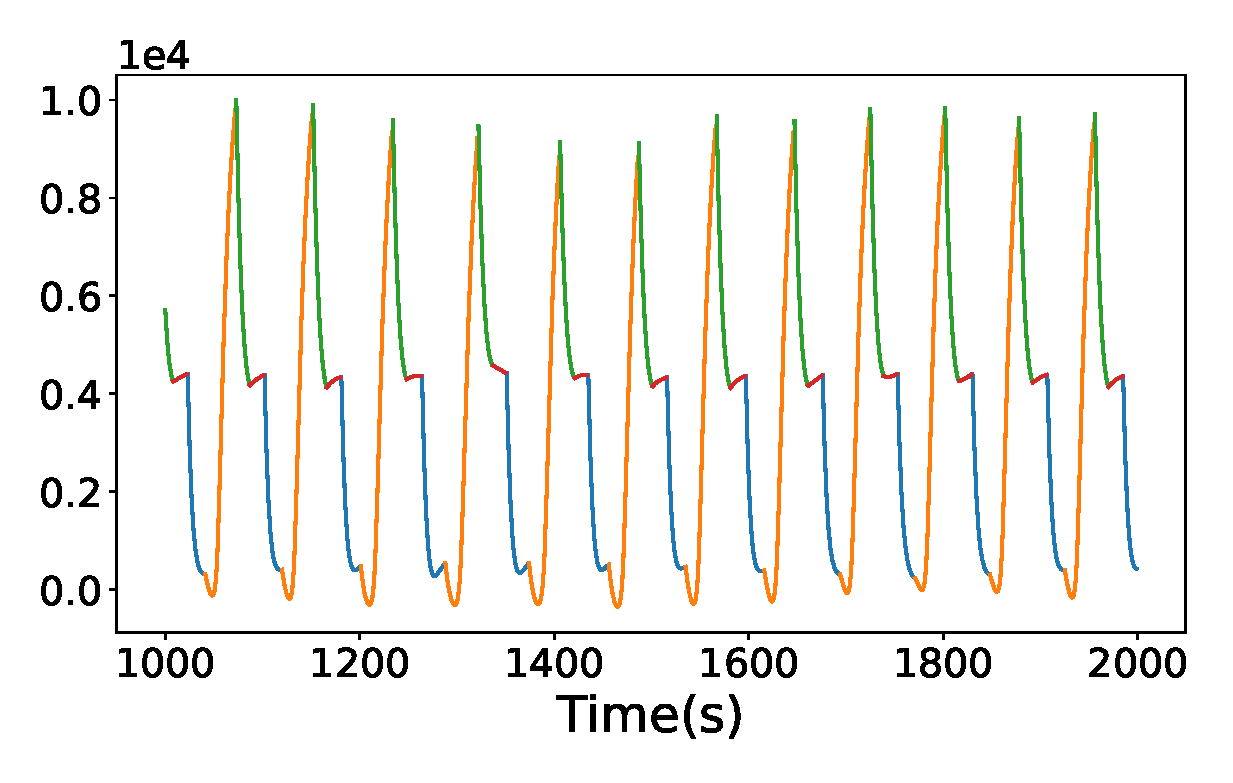
\includegraphics[width=0.45\linewidth]{figures/chapter4/18.eps}} 
\caption{在不同温度下限设定值下的进气口温度的仿真值}
% \caption{The simulations of instant cooling power under different lower boundary of temperature set points}
%\caption{The simulated instant consumed power with different temperature lower boundaries} %图片标题
\label{fig:lowerbound_simulation}
\end{figure*}

% In Fig.~\ref{fig:temperature}, we evaluate the predicted accumulated power consumption, PUE\footnote{PUE\text{ }=${\text { Total Facility Energy }}/{\text { IT Equipment Energy }}$\cite{song2015data}}, and Coefficient Of Performance (COP)\footnote{COP\text{ }=${\text { Cooling Production }}/{\text { Power consumption }}$\cite{song2015data}} within an hour for different $Ti_{\min}$.
在图~\ref{fig:temperature}中, 我们评估了一个小时内,不同$Ti_{\min}$下的预测累积能耗, PUE\footnote{PUE\text{ }=${\text {  总能耗 }}/{\text { 设备工作能耗 }}$\cite{song2015data}}, 以及性能系数(COP)\footnote{COP\text{ }=${\text {制冷量}}/{\text { 制冷能耗}}$\cite{song2015data}}。
PUE代表整个总能耗(制冷能耗与设备能耗的和)与设备能耗的比。
% PUE is the ratio of the total amount of energy used by a data center facility to the energy delivered to computing equipment.
% The more close PUE is to 1, the more energy-efficient the data center is.
% COP is a ratio of the actual produced cooling to required energy consumption.
PUE越接近1,说明整套系统越节能。
COP是实际产生的制冷量与所需能耗的比值。

% When the lower threshold is increased from ${12}^{\circ} \mathrm{C}$ to ${18}^{\circ} \mathrm{C}$, the total energy consumption declines at first and then gradually goes up after certain points.
当温度下阈值从${12}^{\circ} \mathrm{C}$增加到${18}^{\circ} \mathrm{C}$时,制冷系统总能耗先下降然后逐渐上升。
% Since the higher $Ti_{\min}$ setting narrows the gap between the upper and the lower thresholds, which makes the compressor restart more frequently. Even though the restarting process has short duration, compressor has extremely high power. 
由于设置较高的$Ti_{\min}$会缩小上下限之间的差距,使得压缩机更频繁地重启。虽然重启时间较短,但此时压缩机功耗是极高的。
% As a result, from certain point on, the energy consumption accumulated during compressor restarting process accounts for an important portion, and total energy consumption goes up after that. This certain point is actually the optimal $Ti_{\min}$ that we are searching for.
因此,从某一温度开始,由于压缩机重新启动导致的能量消耗占据了制冷总能耗的主要部分,在此之后总能量消耗就会上升。而这一拐点就是寻找的最佳$Ti_{\min}$。
% For the three experiments with different heat loads, the optimal $Ti_{\min}$, where the total energy consumption is minimized are marked in Fig.~\ref{fig:energy}. 
对于三个不同热负荷的数据集,图~\ref{fig:energy}中标出了使总能耗最小的最佳的$Ti_{\min}$。
% In Fig.~\ref{fig:pue}, the optimal temperature thresholds are consistent with the ones in Fig.~\ref{fig:energy}.
% In Fig.~\ref{fig:cop}, COP decreases with the increase of $Ti_{\min}$. 
% The reason is that frequent on-off operations reduce the time for stable cooling. 
在图~\ref{fig:pue}中,最佳温度阈值与图~\ref{fig:energy}中的阈值一致。
在图~\ref{fig:cop}中,COP随着$Ti_{\min}$的增加不断降低。其原因为频繁的压缩机开闭过程会减少了稳定制冷的时间,进而导致单位功耗下产生的制冷量下降。
% We take it for granted that the COP is lower when system is unstable.
% When the cooling system runs unstably for a long time, the COP decreases naturally.
% The decline tendency in COP also explains why the required cooling decreases while the energy consumption increases.
COP的下降趋势也解释了为什么提高温度下限值,所需的冷却量减少而制冷能耗却增加。

% 仿真结果如图.~\ref{fig:temperature}所示,曲线中标出了系统达到最小功耗时的温度下限设定值。
与此同时我们发现,最优温度设定点随负载的变化而变化。热负载越大,最优温度设定值越大。
基于仿真实验推导出的最优温度设置点$Ti^*_{\min}$,表~\ref{tab:power_save_percent}展示了优化温度设定点可以节省的功耗百分比。
根据仿真结果,采用新的温度下限设定值可以节省约6-25\%的能耗,特别对于高热负载情况下的能耗优化是极其显著的。
因为实验\ref{sec:case-study1}中评估了模型预测累积能耗的相对百分比误差小于5\%,可以认为本节对于不同温度下限设定值的仿真结果是有足够可信度。
在未来的工作中,将进一步验证该温度设定策略在实际工业制冷系统中的能耗优化表现。

% The simulations are shown in 图.~\ref{fig:temperature}, and the optimal lower temperature set point, which can achieve the least energy consumption are marked in the curves. 
% It can be found that, optimal temperature set points are varied with the heat load, higher heat load corresponding to higher optimal temperature set points. 
% Based on the inferred optimal set points, the percentage of the saved energy is simulated and shown in \ref{tab:power_save_percent}.
% From results, we find that optimizing the lower boundary set point will produce great energy saving. 
% It is an extremely economical and green improvement of the studied data center, which is supposed to be verified in the future work.

\begin{table}[]
\centering
\caption{optimized power}
\label{tab:power_save_percent}
\begin{tabular}{lcccc}
\hline
\multicolumn{1}{c}{\textbf{不同负载的数据集}} & 1.7k  & 3.8k    & 6.3k  \\ \hline
最优温度设定值(${ }^{\circ} \mathrm{C}$)               & 14   & 15     & 15.5    \\
最大功耗优化比例(\%)              & 6.49 & 10.93  & 25.71\\ \hline
\end{tabular}
\end{table}


% optimized power,best temp set point is the temperature point when the power consumption is the lowest ,max optimized power is compare the lowest power consumption with the truth power consumption



% \begin{table*}[]
% \centering
% \caption{rrse(1.7k)}
% \label{tab:rrse(1.7k)}
% \begin{tabular}{lccc}
% \hline
% \textbf{\%RRSE(1.7k)} & Ti    & PCooling & Power Cooling \\ \hline
% H-ODE                 & 14.32  & 17.34    & 19.37        \\
% ODE-RNN               & 16.33  & 18.86    & 16.79        \\ \hline
% \end{tabular}
% \end{table*}

% \begin{table*}[]
% \centering
% \caption{rrse(3.8k)}
% \label{tab:rrse(3.8k)}
% \begin{tabular}{lccc}
% \hline
% \textbf{RRSE(3.8k)} & Ti    & PCooling & Power Cooling \\ \hline
% H-ODE               & 12.77 & 14.60    & 17.79         \\
% ODE-RNN             & 15.37 & 15.25    & 16.97         \\ \hline
% \end{tabular}
% \end{table*}



% \begin{table*}[]
% \centering
% \caption{rrse(4.2k)}
% \label{tab:rrse(4.2k)}
% \begin{tabular}{lccc}
% \hline
% \textbf{RRSE(4.2k)} & Ti    & PCooling & Power Cooling \\ \hline
% H-ODE               & 13.34 & 15.57    & 18.88         \\
% ODE-RNN             & 17.03 & 18.61    & 17.54         \\ \hline
% \end{tabular}
% \end{table*}

% \begin{table*}[]
% \centering
% \caption{rrse(6.3k)}
% \label{tab:rrse(4.2k)}
% \begin{tabular}{lccc}
% \hline
% \textbf{RRSE(6.3k)} & Ti    & PCooling & Power Cooling \\ \hline
% H-ODE               & 13.07 & 15.65    & 19.29         \\
% ODE-RNN             & 17.75 & 18.61    & 18.23         \\ \hline
% \end{tabular}
% \end{table*}


% \begin{figure}
% \centering
% \subfigure[The time of state-off]{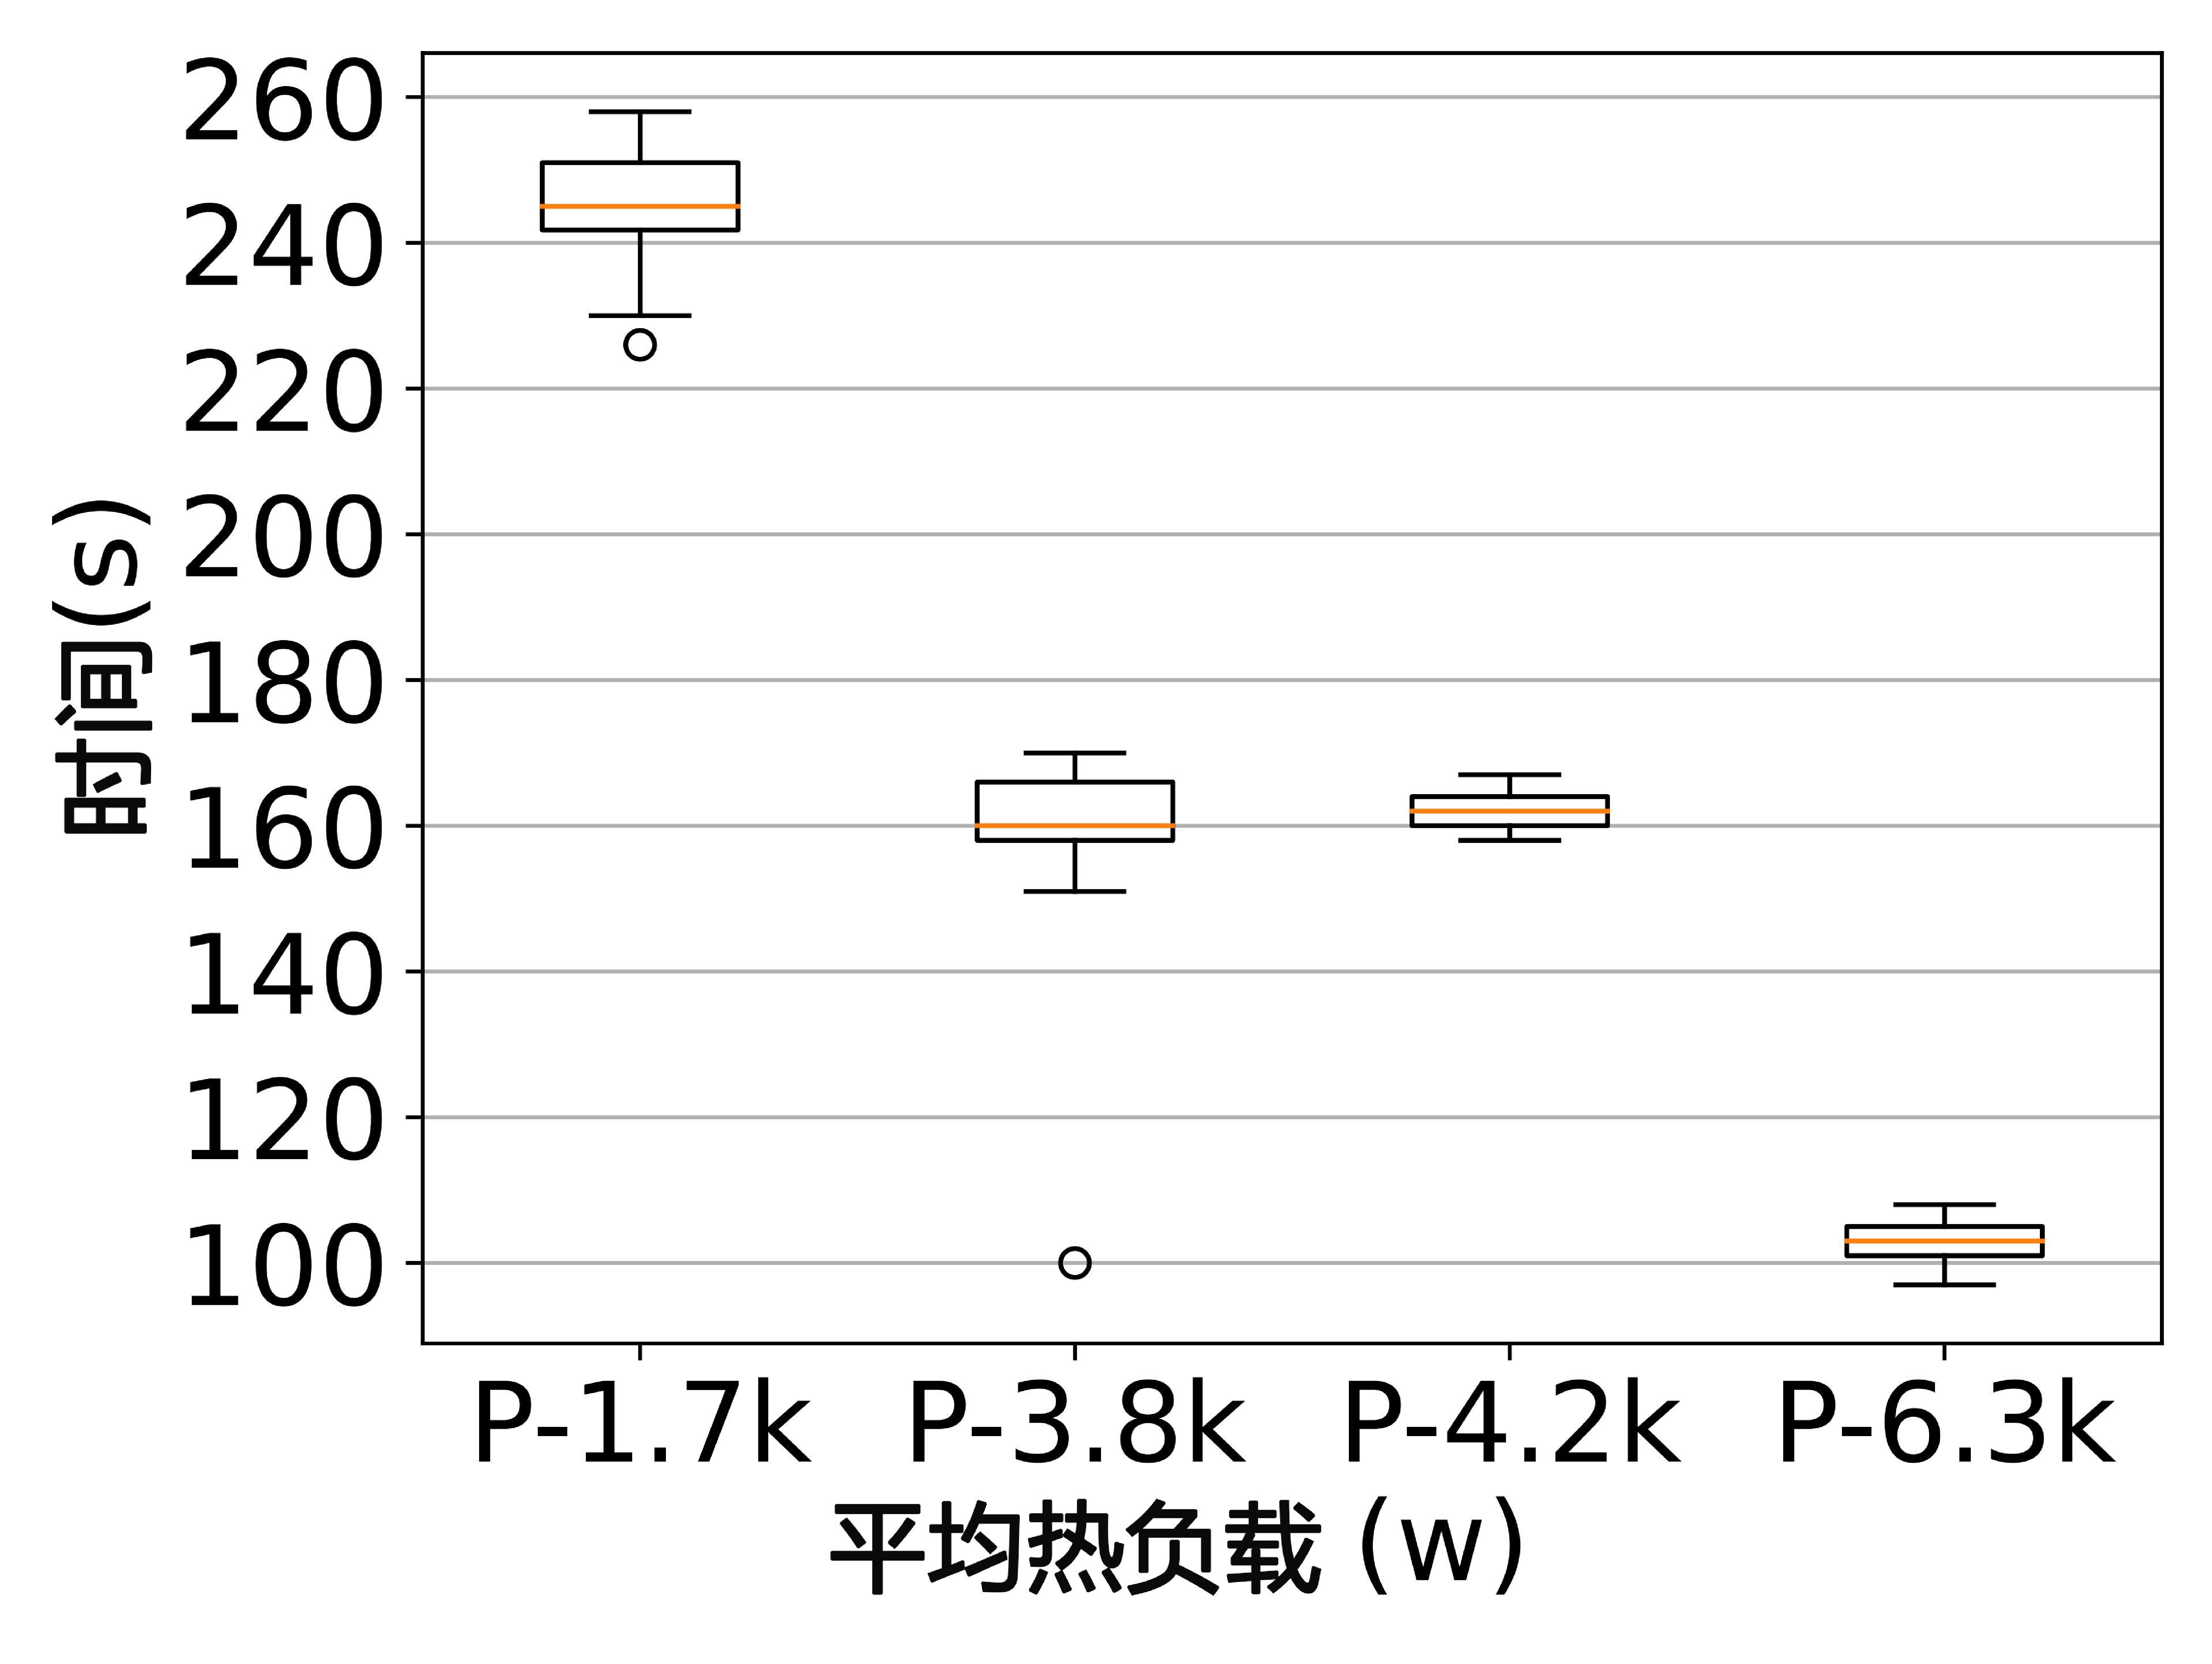
\includegraphics[width=4cm]{figures/chapter4/state1.png}}
% \subfigure[The time of state-on]{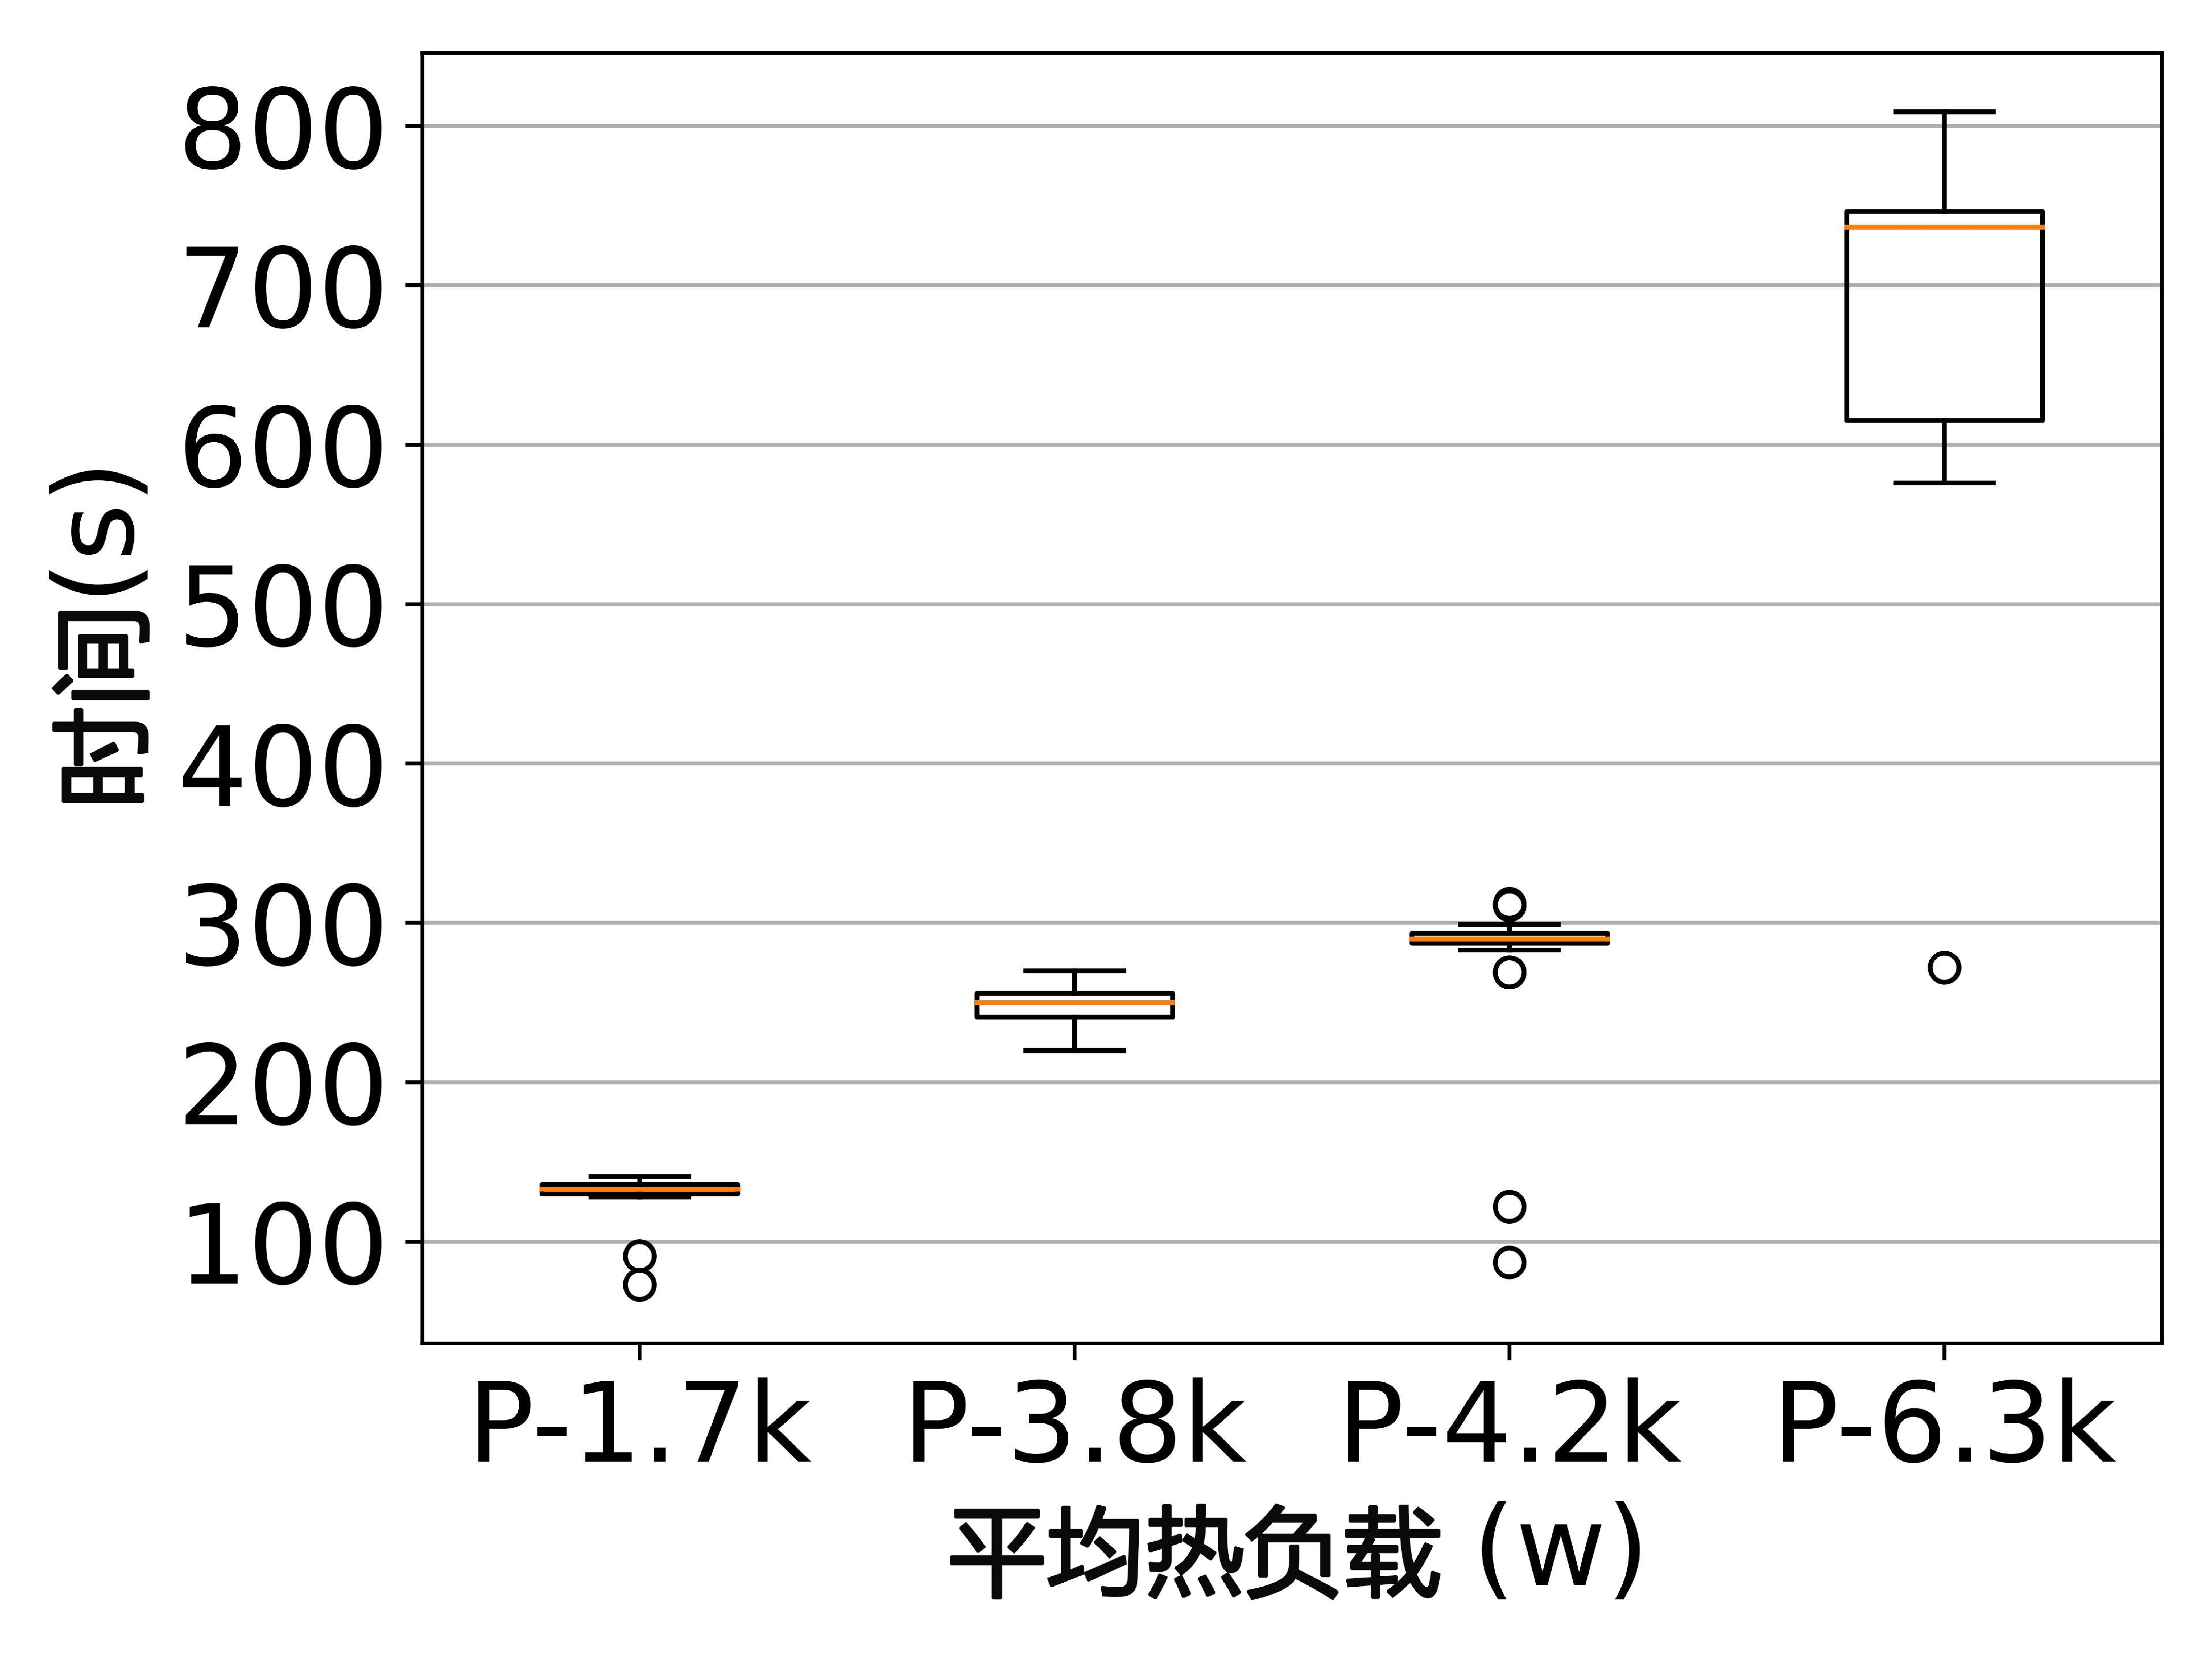
\includegraphics[width=4cm]{figures/chapter4/state4.png}}
% \caption{The data of the four data sets are generated at different power of the server, which are 1.7kw, 3.8kw, 4.2kw and 6.3kw respectively. Compare the duration time of system on and off under different power.} %图片标题
% \label{fig:state}  %图片交叉引用时的标签
% \end{figure}

\begin{figure*}[htb]
    \centering
    \subfigure[制冷能耗]{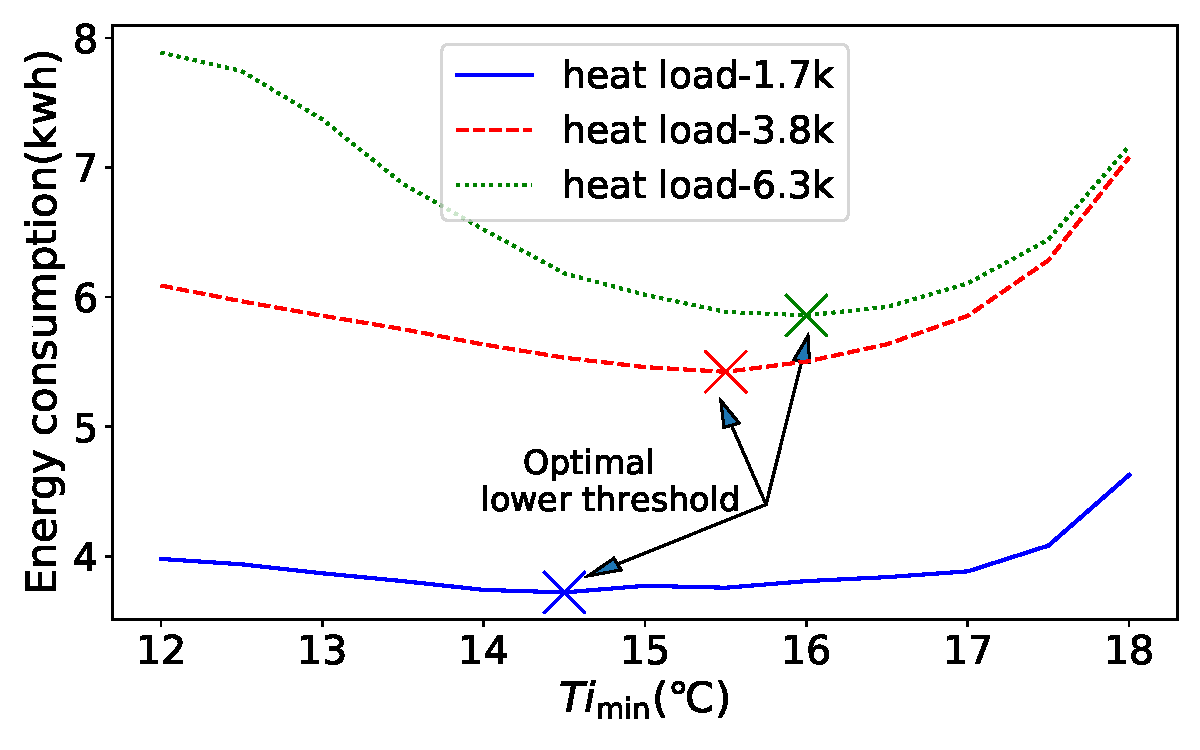
\includegraphics[width=0.7\linewidth]{figures/chapter4/power.pdf}\label{fig:energy}}
    \subfigure[PUE]{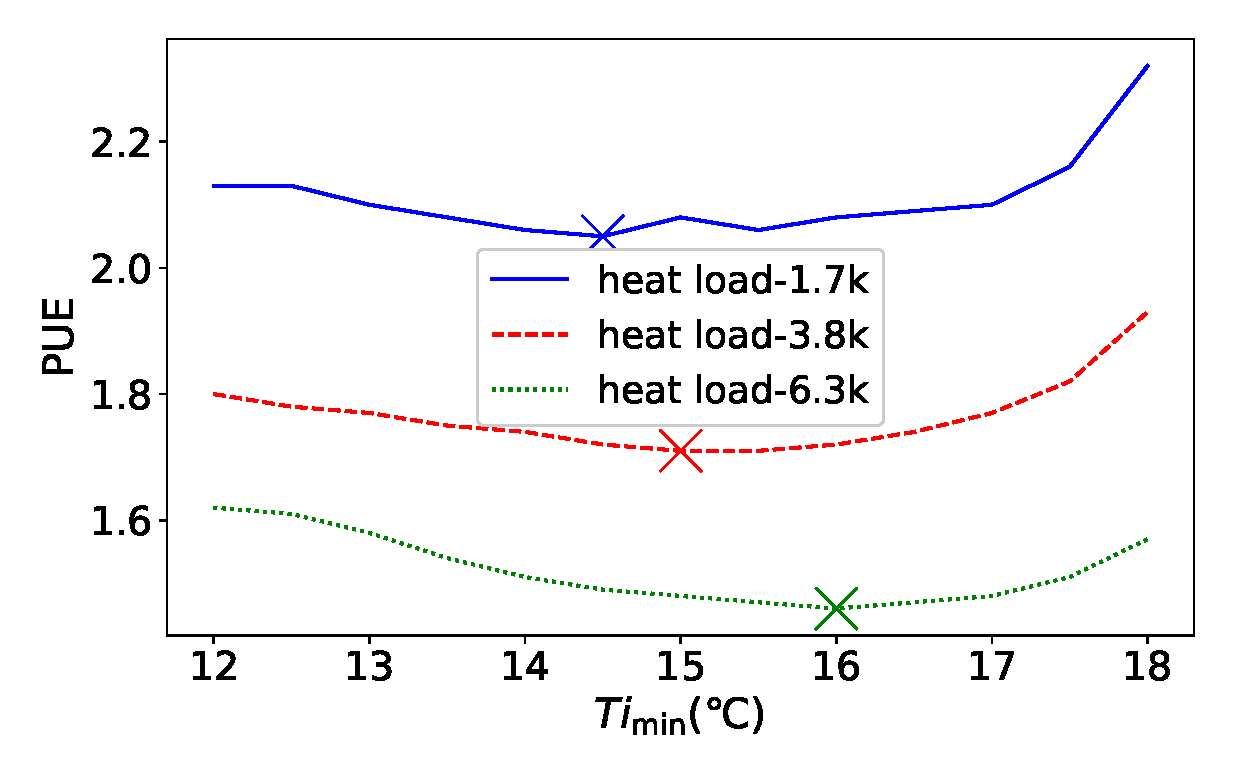
\includegraphics[width=0.7\linewidth]{figures/chapter4/pue.eps}\label{fig:pue}}
    \subfigure[COP]{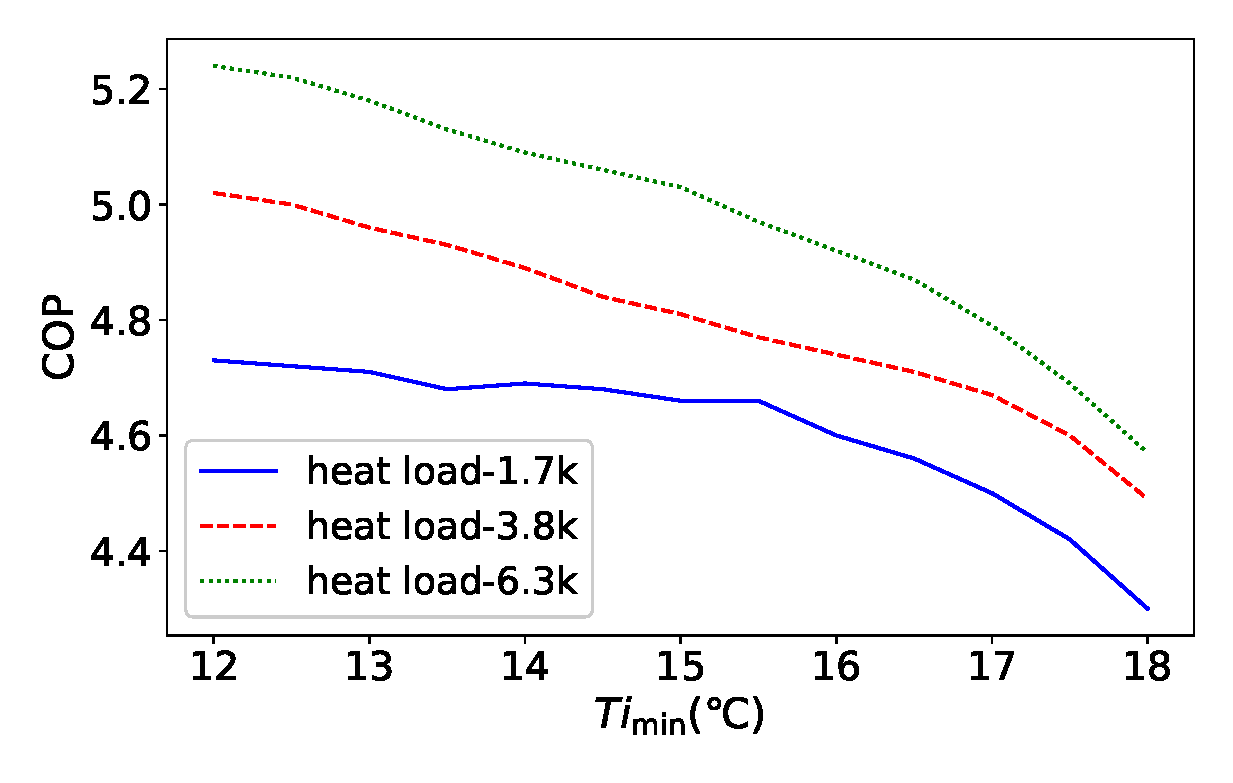
\includegraphics[width=0.7\linewidth]{figures/chapter4/cop.eps}\label{fig:cop}}
    % 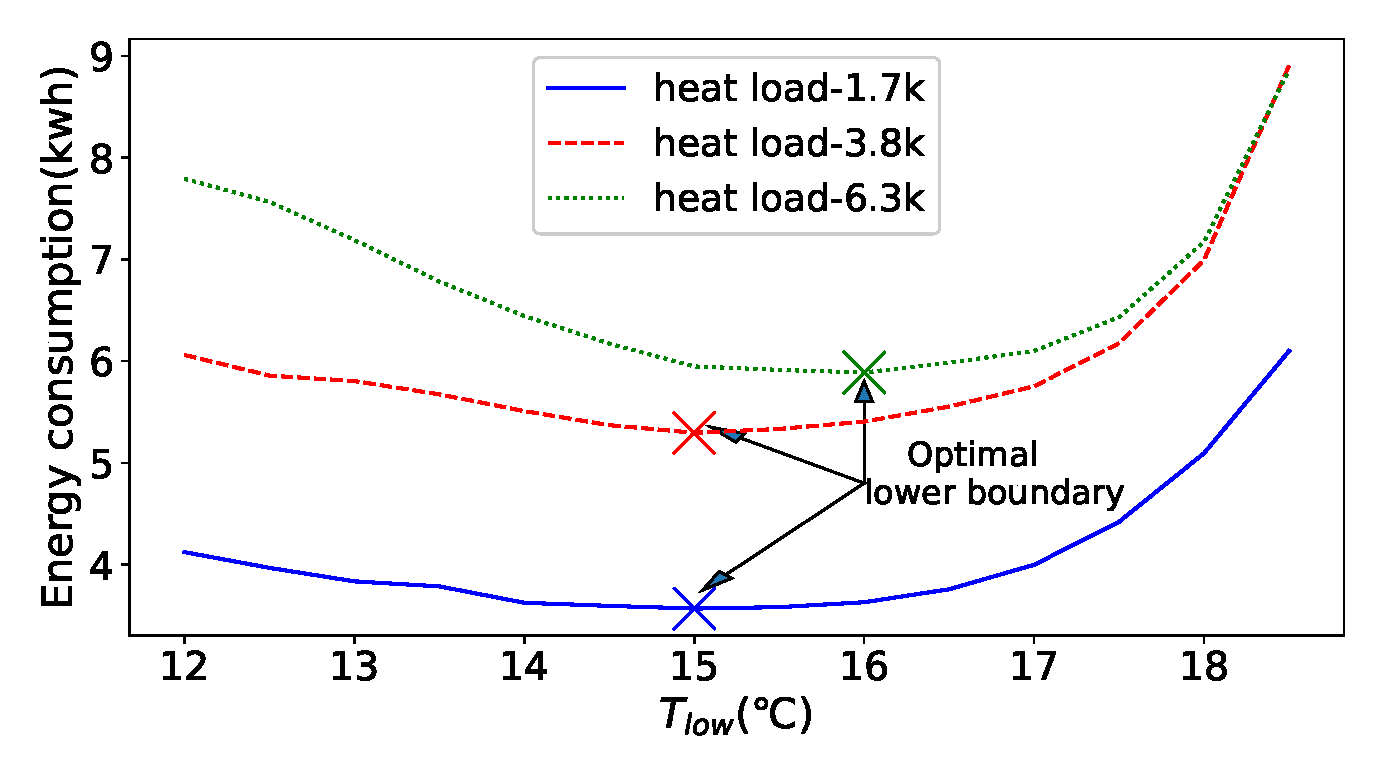
\includegraphics[width=8cm]{figures/temperature.eps}
    \caption{在不同热负载下改变温度设定下限值对功耗、COP、PUE的影响}
    \label{fig:temperature}
    \vspace{-10pt}
\end{figure*}

\section{本章小结}
\label{sec:conclusion}
针对连续时间周期跳变系统的建模预测问题,本文提出了一种基于H-ODENet的AJ-ODEnets模型,同时基于该模型构建了用于系统开环预测的编码器-解码器框架。
% 该模型能够对给定历史序列数据中学习系统中不同阶段下的多输入多输出动态特性,通过给定未来的系统输入能够预测系统的未来输出。
该模型能够对给定的历史序列数据进行编码,在给定未来系统输入序列下仿真预测系统的未来输出。
% 中学习系统中不同阶段下的多输入多输出动态特性,通过给定未来的系统输入能够预测系统的未来输出。
为了使AJ-ODEnet更好地学习不同阶段的动态特性,AJ-ODEnet包含了多个层次常微分方程网络(Hierarchical Neural ODE network), 独立地学习每个阶段下的系统动态特性,并分别建模系统的稳定输出和非稳定输出,同时构建阶段转换预测器以指定各个预测时刻所用的H-ODENet。
作为ODENet的扩展,H-ODENet中的双层结构分别用于估计隐状态的导数和系统输出的导数,并且对于稳定输出和非稳定输出采用不同的导数模块进行建模。
% 基于AJ设计的阶段转换预测器将系统的先验知识集成为转换规则,以提高模型的预测精度和可解释性。
最后,本章利用所提出的基于AJ-ODEnet的编码器-解码器框架建模某一工业制冷系统。与其他方法相比,AJ-ODEnet在对于制冷系统温度、功耗的开环预测问题中表现出了良好性能,并且能够准确地预估阶段转换点。
% Furthermore, we search the optimal lower threshold set points for the inlet temperature for minimizing cooling energy consumption with different heat loads.
此外,依托于训练得到的仿真模型,以最小化不同热负荷下的制冷能耗为目标,我们成功优化了制冷系统的温度下限设定点。
% It is shown that up to 25\% energy can be saved by adopting the optimized settings obtained by the simulations.
仿真结果表明,通过采纳优化后温度阈值设置可以节省高达25%的能耗。
% The proposed AJ-ODENet could be deployed forward to model general continuous-time markov jump systems, future works will be devoted to extend the deterministic stage prediction to markov process.
% 本章所提出的AJ-ODENet可以被应用于一般的连续时间马尔科夫跳跃系统的模型中,未来的工作将致力于将确定性的阶段预测扩展到带有随机性的马尔科夫过程。
% Moreover, instead of designing transition rules manually in complex systems, we consider to further develop more intelligent stage labeling solutions based on unsupervised machine learning methods~\cite{10.1145/3097983.3098060}.





% 此外,基于训练得到的仿真模型实现了对于制冷系统的能耗仿真。实验结果表明,当预测时间超过35分钟时,能够基本消除了相位误差的影响,模型能够较为准确地估计预测时间内的系统能耗。另外,该模型能够仿真触发制冷启动的温度设定值对于系统能耗的影响,进而求解使冷却能耗最小的最优温度设定值。通过对不同服务器负载数据进行模拟,给出了不同负载下的最优温度设定,并预估经过优化的设定值能够节省制冷系统能耗约29\%。


% In this paper, a novel deep learning based framework AJ-ODEnets is proposed, target at modeling periodic and multi-stage industrial complex systems. It is a MIMO framework, at first place, the framework learns the system behavior and stage transitions during given duration of conditional range, then start to predict required variables with given inputs. AJ-ODEnet serves as the key module, which takes in inputs, generates hidden states and appoints the system to switch across different ODEnets. In order to better characterize different and hybrid physical processes, Hierarchical Neural ODE networks (H-ODEnet) are adopted to fit different stages of the system, which contains hybrid stationary and non-stationary structure to deal with complex and more general cases. In addition, prior knowledge is integrated and written as transformation rules into the AJ of Stage Transition Predictor. The option allows improving the model interpretability, and exploring system optimization possibilities. With the features mentioned above, AJ-ODEnet has prominent advantages in simulating multi-stage physical processing. Finally, the proposed AJ-ODEnet framework is implemented on a cooling system of a running data center. Comparing with other methods, AJ-ODEnets achieves better performance in open loop estimation for several operating variables, with accurate results for each stage including the transition point. \\
% Moreover, two applications are realized as use cases. Firstly, the framework is applied to estimate energy consumption for short and long terms cases. Evaluations show that, accurate estimation results can be obtained for prediction duration more than 35 minutes, to get rid of the impact brought by initial points (phrase difference in periodic sequences). Secondly, for the purpose of reducing cooling energy consumption, simulations are conducted by varying lower boundary temperature set points within Stage Transition Predictor to search for the optimal configuration under different heat load
% \chapter{插入参考文献}
% \section{\BibTeX 的使用}
% \BibTeX 是一种格式和一个程序,用于协调LaTeX的参考文献处理。\BibTeX 使用数据库的的方式来管理参考文献. \BibTeX 文件的后缀名为 .bib。 先来看一个例子:
% \begin{quote}
% @article\{name1,\\
% author = \{作者, 多个作者用 and 连接\},\\
% title = \{标题\},\\
% journal = \{期刊名\},\\
% volume = \{卷20\},\\
% number = \{页码\},\\
% year = \{年份\},\\
% abstract = \{摘要, 这个主要是引用的时候自己参考的, 这一行不是必须的\}\\
% \}\\

% @book\{name2,\\
% author ="作者",\\
% year="年份2008",\\
% title="书名",\\
% publisher ="出版社名称"\\
% \}
% \end{quote}
% 说明:第一行@article 告诉 \BibTeX 这是一个文章类型的参考文献,还有其它格式, 例如 article, book, booklet, conference, inbook, incollection, inproceedings,manual, misc, mastersthesis, phdthesis, proceedings, techreport, unpublished 等等。接下来的"name1",就是你在正文中应用这个条目的名称。其它就是参考文献里面的具体内容啦。
% \section{在\LaTeX 中使用\BibTeX }
% 为了在LaTeX中使用BibTeX 数据库, 你必须先做下面三件事情:
% \begin{enumerate}
% \item 设置参考文献的类型 (bibliography style). 标准的为 plain:\\
%   $\backslash$bibliographystyle\{plain\}\\
% 将上面的命令放在 \LaTeX 文档的 $\backslash$begin\{document\}后边. 其它的类型包括:\\
% unsrt – 基本上跟 plain 类型一样,除了参考文献的条目的编号是按照引用的顺序,而不是按照作者的字母顺序。\\
% alpha – 类似于 plain 类型,当参考文献的条目的编号基于作者名字和出版年份的顺序。\\
% abbrv – 缩写格式。
% \item 标记引用 (Make citations). 当你在文档中想使用引用时, 插入\LaTeX 命令$\backslash$cite{引用文章名称}。"引用文章名称" 就是前边定义@article后面的名称.
% \item 告诉LaTeX生成参考文献列表,在 LaTeX 的结束前输入$\backslash$bibliography{bibfile}。这里bibfile 就是你的 BibTeX 数据库文件 bibfile.bib .
% \end{enumerate}

% \section{运行 \BibTeX}
% 分为下面四步:
% \begin{enumerate}
% \item 用LaTeX编译你的 .tex 文件 , 这是生成一个 .aux 的文件, 这告诉 \BibTeX 将使用那些应用;
% \item 用\BibTeX 编译 .bib 文件;
% \item 再次用\LaTeX 编译你的 .tex 文件,这个时候在文档中已经包含了参考文献,但此时引用的编号可能不正确;
% \item 最后用 \LaTeX 编译你的 .tex 文件,如果一切顺利的话, 这是所有东西都已正常了.
% \end{enumerate}

% \section{本论文参考文献格式}
% 北京科技大学博士论文的参考文献要求符合国家标准“GB/T7714-2005文后参考文献著录规则”。本模板中已包含了关于符合此要求的gbt7714-2005.bst文件,只需要将参考文献类型设置为$\backslash$bibliographystyle\{gbt7714-2005\}即可。



%第五章
% \usepackage{colortbl}  %彩色表格需要加载的宏包
% \usepackage{xcolor}
% \usepackage{array}   %对表列和表格线的设置需要用到array宏包
% \chapter{ODE-RSSM:利用非均匀采样数据建模随机状态空间模型}
\chapter{基于深度常微分马尔可夫模型的随机非确定性系统建模}
\renewcommand{\b}{\boldsymbol}   % This command is specifically forbidden
% \renewcommand{\b}[1]{\boldsymbol{#1}}
\newcommand{\zt}{\boldsymbol{z}_{t_i}}
\newcommand{\st}{\boldsymbol{s}_{t_i}}
\newcommand{\hti}{\boldsymbol{h}_{t_i}}
\newcommand{\thti}{\boldsymbol{\tilde{h}}_{t_i}}
\newcommand{\ut}{\boldsymbol{u}_{t_i}}
\newcommand{\yt}{\boldsymbol{y}_{t_i}}
\newcommand{\ct}{\boldsymbol{c}_{t_{i}}}
\newcommand{\rt}{\boldsymbol{r}_{t}}

\newcommand{\ztm}{\boldsymbol{z}_{t_{i-1}}}
\newcommand{\stm}{\boldsymbol{s}_{t_{i-1}}}
\newcommand{\htm}{\boldsymbol{h}_{t_{i-1}}}
\newcommand{\utm}{\boldsymbol{u}_{t_{i-1}}}
\newcommand{\ytm}{\boldsymbol{y}_{t_{i-1}}}
\newcommand{\ctm}{\boldsymbol{c}_{t_{i-1}}}
\newcommand{\thtm}{\boldsymbol{\tilde{h}}_{t_{i-1}}}

\newcommand{\ztp}{\boldsymbol{z}_{t_{i+1}}}
\newcommand{\stp}{\boldsymbol{s}_{t_{i+1}}}
\newcommand{\htp}{\boldsymbol{h}_{t_{i+1}}}
\newcommand{\utp}{\boldsymbol{u}_{t_{i+1}}}
\newcommand{\ytp}{\boldsymbol{y}_{t_{i+1}}}
\newcommand{\ctp}{\boldsymbol{c}_{t_{i+1}}}
\newcommand{\thtp}{\boldsymbol{\tilde{h}}_{t+i}}




% For the complicated input-output systems with nonlinearity and stochasticity,
% deep state space models(SSMs) are effective for learning temporal inference model and generative model, which are of great significance for representation, forecasting, and control in online scenario.
% However, most deep SSMs are designed for discrete sequences and inapplicable when the observations are irregular in time.
% To solve the problem, we propose a novel continuous-time SSM named Ordinary Differential Equation Recurrent State Space Model(ODE-RSSM), which introduces both stochastic and deterministic paths in SSM and utilizes the ODE-Net to model the evolution of hidden state between adjacent time points in continuous-time domain. 
% We also incorporate the Parallel Reuse latent overshooting technique in training stage to improve the long-term prediction without raising training time.
% Through comprehensive experiments with three input-output system datasets, we show continuous-time ODE-RSSM outperforms the discrete-time SSMs and achieve remarkable performance on reconstructions and predictions tasks for evenly system observations.

% 对于同时具有非线性、非确定性(Uncertainy)及随机性(stochasticity)的复杂输入输出系统,
% 深度状态空间模型(SSMs)作为一种支持在线处理的参数模型,在学习状态推理和状态生成方面十分有效。
% 广泛应用于复杂系统的表示、预测和控制等问题中。
% 然而,大多数深度状态空间模型假设训练数据及预测数据是均匀采样的,当观测数据的采样时间非均匀时,离散时间状态空间模型无法适用。
% 为了解决这一问题,本章提出了一种新颖的连续时间深度状态空间模型——常微分方程循环状态空间模型(Ordinary Differential Equation Recurrent State Space Model, ODE-RSSM),该模型在状态转换过程中同时引入了随机和确定性路径,并利用ODE-Net建模连续时域下相邻采样时间点之间的隐状态变化。
% 另外,在训练阶段,为了使该模型能够支持批量并行推理与训练,需要解决batch中不同常微分方程积分区间不一致的问题。因此本章提出了一种批量常微分方程并行求解方法,能够高效地求解多个积分区间不同的常微分方程。
% 最后为了提升模型的长期预测精度,本章在模型训练阶段引入了采样状态重用的隐空间超调技术,相比于传统的隐状态超调技术能够以更低的训练开销提升长期预测精度。
% 最后,本章通过三个输入输出系统数据集对所述模型及改进进行评估。实验表明在非均匀采样下的随机系统预测任务上,ODE-RSSM无论是在处理非均匀采样方面还是建模系统随机性方面均具有良好表现,预测精度显著优于离散时间状态空间模型以及带有确定性状态演变的连续时间模型。

% Model prediction control(MPC) based on deep learning framework is a powerful approach for controlling unknown complicated industrial system.
% With the physics-informed prior knowledge and the offline operating dataset, deep neural prediction model is learned and regarded as a simulation of controlled system.
% In the environment of online production , the prediction model analysis the past system trajectories and forecasts the future system outputs in long range under optimized future system inputs.
% With a deterministic objective function, the optimal sequential system inputs are solved and the first element is adopted to control the system.
% The procedure above is recursively executed with a given period, which is shorter than the length of prediction range.

% In modern industrial scenarios, sufficient offline data from system promote the employment of MPC in some previous studies\cite{Member2019}.
% However, several challenges restrict the employments and effectiveness of MPC in some complicated industrial system.

% System identification based on deep learning exploits the advantages of deep neural networks (DNN) to identify black-box system dynamics from offline input-output data.
% As a substitution of the actual system, the learned model is generally utilized for prediction, model prediction control and model-based reinforcement learning (MBRL),
% However, there are several common challenges in modelling real systems:
% First, many neural-network-based system identification models in previous studies only model the deterministic dynamics.
基于深度学习的系统识别方法结合了深度神经网络在建模非线性复杂函数的优势,实现利用离线输入输出数据识别未知参数结构的黑盒系统动态。
训练后的模型可以作为实际系统的近似替代,以支撑仿真预测、模型预测控制和基于模型的强化学习(Model-based Reinforcement learning, MBRL)等下游决策优化任务。
然而,在建模真实工业系统时经常面临如下挑战:
首先,在以往的研究中,许多基于神经网络的系统辨识模型属于确定性模型,无法对系统状态转移的随机性以及不完备观测造成的确定性进行建模。因此,此类模型仅适用于对确定性动态系统进行建模,不适用于带有随机性或观测空间存在非确定性的系统。
% , which can not learn the systems that suffers from high uncertainty the stochastic property. 
% While most system suffers from high uncertainty. 
% Deterministic models can not learn the systems that suffers from high uncertainty the stochastic property.
% In the meanwhile, some MBRL methods also require the stochastic identified model for sampling and exploration.

% Second, messy or irregular sampling data is ubiquitous in practical industrial applications\cite{kidger2021}. 
% % Different channels may be observed at different frequencies, data may be missing, sampling interval may be of variable lengths, and so on. 
% % Though the discrete-time
% The discrete-time models defined on the assumption of evenly sampling intervals are restricted in real-time industrial system, especially in online scenarios where offline interpolations are incapable.
% Third, in some complicated industrial system, the influences from inputs on system outputs are not instantaneous. 
% It is a critical issue to guarantee the robustness and accuracy of long-term open loop prediction because of the existed long-time delay.
其次,在实际工业应用中,时间间隔不均匀的采样数据是普遍存在的\cite{kidger2021}。依赖于均匀采样间隔假设的离散时间模型不便于从非均匀采样数据进行学习。尽管可以采用离线插值的方式强行调整训练集数据的采样间隔,不过模型仍要求推理数据和训练数据的采样间隔需保持一致,因此在实时工业应用中此类模型存在一定的局限性。

第三,在一些复杂的工业系统中,系统输入对系统输出的影响不是瞬时的。
系统关键指标受外部输入的影响变化可能存在长时间的滞后性,当使用辨识的模型进行长期开环预测时,如何保证长期预测结果的鲁棒性和准确性对模型的设计及训练提出了更高的要求。
% Because there is a long time-delay in some complicated control processes, 
% Because there is a long time-delay in some complicated control processes, it is inappropriate to learn the input-output functions directly without any state space and temporal encoding.
% Finally, the identification model is always required to work in online mode for handling continuous streaming data and arbitrary predicted range~\cite{VSDN_Liu2020}.
% This further restricts the employments of some end-to-end encoder-decoder models~\cite{Rubanova2019,Yildiz2019}, but prefers to choose the models with recurrent state updating.
最后,在某些应用场景下,训练完成的识别模型需要工作在在线模式下,用于处理连续的流式数据,且其预测范围及输入序列长度可能是动态变化的~\cite{VSDN_Liu2020}。
这一要求进一步限制了某些端到端编码器-解码器模型的使用~\cite{Rubanova2019,Yildiz2019},
更倾向于选择具有循环状态更新的模型。
% In some specific tasks, such as online control, the prediction model is required to be working in online mode for handling streaming data, just like the recurrent neural network which updates internal state recursively.
% In some specific tasks, such as online control, the prediction model is required to be working in online mode for handling streaming data, just like the recurrent neural network which updates internal state recursively.
% Therefore, it is a critical issue to guarantee the long-term forecasting of the prediction in MPC.

% One or parts of issues mentioned above are indeed solved by previous studies.
% However, as far as we known, none of existed works could tackle all of the problems simultaneously.
% In this paper, we propose the Ordinary Differential Equation Recurrent State Space Model(ODE-RSSM), a stochastic transition model defined in continuous-time(CT) domain to learn the dynamics with both stochasticity and long-term delay from irregular sample data. 
% The model extends the RSSM for evenly spaced sequential data by incorporating an ODE-Net in the state evolution.
% Furthermore, we introduce an efficient parallel latent overshooting technique in training phase to improve the long-term prediction. 
% We evaluate 
% The performances of the proposed model in long-term open-loop prediction are evaluated in three system identification datasets, two public datastes and one private dataset.

现有研究成果往往只能解决上述问题中的一个或几个。然而,目前尚没有某一模型能够同时解决上述所有问题。
因此,本文提出常微分方程循环状态空间模型(Ordinary Differential Equation Recurrent State Space Model, ODE-RSSM),该模型一个定义在连续时间(CT)域中的随机过渡模型,
该模型描述了系统状态在连续时间域下的随机演化,能够用于从不规则样本数据中学习具有随机性和长时滞特性的动态系统。
具体地,相比于离散时间域下的循环状态空间模型,ODE-RSSM通过在状态演化中加入ODE-Net以描述模型内部状态对时间的导数,以此建模任意长度时间间隔的状态演变。
另外,在训练阶段,为了使该模型能够支持批量并行化推理与训练,需要解决同一数据批中求解时间点彼此不同、积分区间彼此不一致的问题。
因此本章提出了一种批常微分方程并行求解方法,通过构造辅助常微分方程以对其各常微分方程的求解时间点,进而利用现有的深度学习框架高效地求解多个积分区间不同的常微分方程。
此外,本章在训练阶段引入了一种计算复杂度更低的隐空间超调技术,在不显著增加时间复杂度的情况下有效改善模型的长期预测性能。
在实验环节,我们在共3个系统辨识数据集(2个公共数据集和1个私有数据集)上评估了所述模型在长期开环预测问题中的性能。实验表明在非均匀采样下的随机系统预测任务上,ODE-RSSM无论是在处理非均匀采样方面还是建模系统随机性方面均具有良好表现,预测精度显著优于离散时间状态空间模型以及带有确定性状态演变的连续时间模型。相比于其他基于神经网络的系统建模方法,本章提出模型的优势如表\ref{tab:c5_comparison}所示。
\begin{table}[t]
    \centering
    \caption{本章提出方法与现有系统建模方法的对比}
    \label{tab:c5_comparison}
    \begin{tabular}{c|ccc}
    \toprule 
     模型         & 随机性                                 & 非均匀采样                   & 在线预测                           \\ \hline 
    RNN       &  {\XSolidBrush}                        &  {\XSolidBrush}                        &   {\Checkmark} \\
    RSSM           &  {\Checkmark}                          &  {\XSolidBrush}                        &  {\Checkmark}                        \\
    Time-Aware RNN &  {\XSolidBrush}                        &  {\Checkmark}                          &  {\Checkmark}                        \\
    % SNODE &  {\XSolidBrush}                        &  {\Checkmark}                          &  {\Checkmark}                        \\
    ODE-RNN,SNODE        &  {\XSolidBrush}                        &  {\Checkmark}                          &  {\Checkmark}                        \\
    Latent SDE     &  {\Checkmark}                          &  {\Checkmark}                          &  {\XSolidBrush}                      \\
    \textbf{ODE-RSSM}       &  {\Checkmark}                          &  {\Checkmark}                          &  {\Checkmark}                        \\
    \bottomrule
    \end{tabular}
    \end{table}
    

% Furthermore, we utilize the DcspNet to model a real thickening system and  MPC framework whick 
% Furthermore, a MPC control policy is implemented based on DcspNet and cross entropy optimization method(CEM) to solve the process control problem of thickening system.

% To learn continuous-time stochastic dynamics from irregular sampled data, this paper provides a continuous-time state space model that incorporates the ODE-Net in the state evolution.

本章所述工作的核心贡献总结如下:
% Key contributions of this work are summarized as follows:
\begin{enumerate}
\item 本章提出了ODE-RSSM模型,作为深度状态空间模型的扩展,该模型能够利用不均匀采样数据识别具有随机性和长时延特性的输入输出系统。
\item 为了改善模型的长期预测,本章在ODE-RSSM的训练阶段引入了采样状态重用的隐空间超调技术以提升模型的长期预测能力。
\item 本章使用三个输入/输出系统数据集对ODE-RSSM模型的预测性能和所述加速效果进行了评估。其中一个数据集导出于具有明显时滞和随机特性的工业浓密系统。该数据集为首次公开的私有数据集。

    % The code is publicly available on github\footnotemark[1].
\end{enumerate}

% \footnotetext[1]{https://github.com/y18810919727/SE-VAE}
本章的结构组织如下:
本章\ref{sec:related_work}节对本章相关工作进行简介。
本章\ref{sec:background}节对基于变分编码机模型的系统建模方法进行间接。
本章\ref{sec:oderssm}节详细介绍了ODE-RSSM的模型细节及训练方法。
本章\ref{sec:experiment}节详述了实验设计、实验结果、以及实验结果讨论。
本章\ref{sec:discussion}节讨论本文模型的局限及其潜在应用。
最后,\ref{sec:conclusion}节对本文研究工作做出总结。

% 本章\ref{sec:}节给出了变量符号定义以及描述了周期性多阶段系统预测问题的形式化描述。
% 本章\ref{sec:h-ode}节介绍了分层常微分方程网络的定义及结构,以及如何将其用于学习同时带有稳定和非稳定时间序列输出的动态过程。
% 本章\ref{sec:dfa-odenet}介绍了DFA-ODEnet框架,并详细阐述了连续时间域下的状态转移方程、关键模块结构和持续时间预测器的损失函数定义等内容。
% 本章\ref{sec:encoder_decoder}给出了基于DFA-ODEnet模型的编码器解码器框架及其训练方法。
% 本章\ref{sec:evalutaion}节介绍了将所述编码器解码器框架应用于模拟某实际数据中心中,带有多维输入输出的制冷系统。模型能够根据制冷系统的输入对其功耗以及出气口气体温度变化进行模拟预测,同时能够实现不同制冷启动温度配置下的功耗仿真与优化。
% 最后,\ref{sec:conclusion}节对本章工作做出了总结,并对未来的研究研究方向做出了讨论。


% In some real industrial systems, the collection data 

% \section{前置知识}
% \section{常微分方程-循环状态空间模型}
\section{问题形式化描述}
% For an input-output system, we sample the system trajectories irregularly and define the sequential system inputs as  $\{\ut\}_{i=1}^{N}$ and system outputs as  $\{\yt\}_{i=1}^{N}$, where $t_i$ is the sampling time point of the $i$-th position and $N$ is the complete sequence length.
对于任一输入输出系统,
对其非均匀采样数据进行定义,包括序列系统输入为$\{\ut\}_{i=1}^{N}$,以及序列系统输出为$\{\yt\}_{i=1}^{N}$,其中$t_i$为第$i$个位置数据点的采样时间,$N$为完整序列长度。
本文假设对于各维度输入和各维度输出的采样都是同步地。
% 我们对系统轨迹进行非规则采样,定义顺序系统输入为$\{\ut\}_{i=1}^{N}$,系统输出为$\{\yt\}_{i=1}^{N}$,其中$t_i$为$i$-th位置的采样时间点,$N$为完整序列长度。

% we define the time index $t_i$ to denote the sampling time point of the $i$-th position.
% The system inputs and outputs are denoted as $\{\ut\}_{i=1}^{N}$ and $\{\yt\}_{i=1}^{N}$.
% To identify the dynamical system from evenly sampled sequences, we introduce deep state space model, named ODE-RSSM, with latent variables $\zt$ to identify the evolution of dynamical system.
% In the meanwhile, we also follow the basic RSSM\cite{Hafner2019} and introduce a deterministic path with variable $\hti$ in the learned parametric system.
% Similar to the RSSM\cite{Hafner2019} model, the latent states in the proposed ODE-RSSM consist of both deterministic part $\hti$ and stochastic part $\zt$.
本章将具有随机非确定性的系统表示为包含随机隐变量的受控状态空间模型。
% 与RSSM\cite{Hafner2019}模型相似,
模型的隐状态由确定性部分$\hti$和随机部分$\zt$共同组成。
为了描述简便,本章定义$\boldsymbol{s}_{t_{i}}=[\boldsymbol{z}_{t_{i}},\boldsymbol{h}_{t_{i}}]$用于表示$t_i$时刻完整的隐状态。
该序列隐变量描述了系统输出在受控输入下的条件生成过程。
% 以循环状态空间模型(Recurrent State Space, Model, RSSM)~\cite{Hafner2019}为例,模型的内部的更新状态同时包括确定性变量$\b{h}_{i}$和随机变量$\b{z}_{i}$。
利用生成模型参数$\theta$,定义序列隐变量和观测值的联合概率如下:
\begin{equation}
\begin{aligned}
p_{\theta}\left(\b{y}_{1: N}, \b{z}_{1: N},\right.&\left.\b{h}_{1: N} \mid \b{u}_{1: N}, \b{h}_{0}\right)=\prod_{i=1}^{N}
p_{\theta}\left(\b{y}_i \mid \b{z}_i, \b{h}_i\right) \times \\
& \times p_{\theta}\left(\b{z}_i \mid \b{h}_i\right) \widetilde{p}_{\theta}\left(\b{h}_i \mid \b{u}_{i-1},\boldsymbol{z}_{i-1}, \b{h}_{i-1}\right)
\end{aligned}
\label{equ:discrete_rssm}
\end{equation}
% For simplicity, we define $\boldsymbol{s}_{t_{i}}=[\boldsymbol{z}_{t_{i}},\boldsymbol{h}_{t_{i}}]$ to denote the complete latent state at time point $t_i$.
% The purpose of the ODE-RSSM is to learn a deep temporal generative model, which consist of a inference model for inferring the sequential latent states $\{\st\}_{i=1}^{N}$ given both system inputs and outputs, and a generative model for predicting the distribution of $\{\yt\}_{i=1}^{N}$ given system inputs $\{\ut\}_{i=1}^{N}$

% 类似于原始的变分自编码器,基于变分自编码机的系统辨识模型通过引入了序列级隐变量,表示系统输出在受控输入下的条件生成过程。
本章提出的ODE-RSSM为时序变分自编码机模型,模型包括生成模块和推断模块两部分。
推断模块能够在给定系统输入和输出的情况下推断序列隐状态$\{\st\}_{i=1}^{N}$,其生成模型能够在给定系统输入$\{\ut\}_{i=1}^{N}$下,识别$\b z_{1:N}$和$\b h_{1:N}$的变化,进而
预测系统输出$\{\yt\}_{i=1}^{N}$的条件分布.
% 在式\eqref{equ:discrete_rssm}中,$\b z_{1:N}$和$\b h_{1:N}$的变化用于识别给定输入信号$\b u_{1:N}$下,模型的内部状态转换过程。
% The model, meanwhile, could predict the $\yt$ under the condition of known $\ut$.

\section{常微分方程网络-循环状态空间模型}

% In the deep state space models, the evolution of latent states and the projection of observable variables are modeled as parametric deep neural networks.
% Similar to the vanilla variational auto-encoder, VAE-based system modelling methods introduce stochastic latent variables in  the internal states of sequential models. 

% The deterministic transition $\widetilde{p}_{\theta}(\boldsymbol h_{i}|\cdot)$ is a delta distribution and modelled by a deterministic RNN.
% The conditional prior of the stochastic latent state $p_{\theta}\left(\boldsymbol{z}_{t} \mid \boldsymbol{h}_{t}\right)$ and decoder $p_{\theta}\left(\boldsymbol{y}_{i} \mid \boldsymbol{h}_{i}, \boldsymbol{z}_{i}\right)$ are modelled as parametric gaussian distributions.
% In equation \eqref{equ:discrete_rssm}, the evolution of $\b z_{1:N}$ and $\b h_{1:N}$ approximates the state transitions under the input signal $\b u_{1:N}$ in the identified model.

\label{sec:oderssm}
% \subsection{Preliminary}
% For an evenly spaced sequence with length $N$, we define the time index $t_i$ to denote the sampling time point of the $i$-th position.
% With the inspiration from RSSM\cite{Hafner2019}, the latent states in the proposed ODE-RSSM consist of both deterministic parts $\hti$ and stochastic parts $\zt$.
\begin{figure*}[ht]
\subfigure[生成模型]{
\begin{minipage}[t]{0.64\linewidth}
\centering
% \hspace{-22pt}
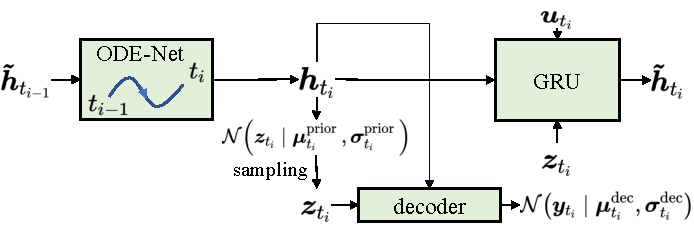
\includegraphics[width=0.9\linewidth]{figures/chapter5/generation.pdf}
%\caption{fig1}
\end{minipage}
\label{fig:generation}
}%
\subfigure[推理模型]{
\begin{minipage}[t]{0.36\linewidth}
\centering
% \hspace{-22pt}
\includegraphics[width=0.9\linewidth]{figures/chapter5/inference.pdf}
%\caption{fig1}
\end{minipage}
\label{fig:encoder}
}%
\centering
\caption{ODE-RSSM中的生成过程和推理过程}
\label{fig:model_fig}
\end{figure*}
% In this section, we first introduce the components of the ODE-RSSM from two aspects: generative process and inference process, as shown in Fig.~\ref{fig:model_fig}.
本节首先介绍ODE-RSSM的生成模型和推断模型,如图~\ref{fig:model_fig}所示。
在生成模型中,在给定系统输入的情况下,模型通过组合门控循环单元(Gate Recurrent Unit, GRU)和ODE网络建模隐状态的转移过程。
为了训练生成模型参数$\theta$, 本章通过引入近似后验编码器 $q_{\phi}\left(\boldsymbol{z}_{i} \mid \boldsymbol{y}_{i}, \boldsymbol{h}_{i}\right)$对隐变量的真实后验分布进行近似,以最大化证据下限(Evidence Lower Bound, ELBO)的方式协同训练参数 $\phi$ 和$\theta$。
另一方面,我们在训练阶段进一步引入隐空间超调技术\cite{Hafner2019}用于改善模型的多步预测。
为了减少引入隐空间超调带来的额外时间开销,进而优化训练效率。本章通过重用临时采样状态的方式显著减少了求解多步KL散度的时间复杂度。

% 在本章提出的ODE-RSSM模型中,
% 将确定性转移函数$\widetilde{p}_{\theta}(\b h_{i}|\cdot)$定义为一德塔(Delta)分布,由一个确定性的循环神经网络进行建模。
% 随机隐状态$p_{\theta}\left(\b {z}_{t} \mid \b {h}_{t}\right)$和解码网络$p_{\theta}\left(\b {y}_{i} \mid \bold {h}_{i},\b {z}_{i}\right)$的条件分布均为参数化的高斯分布。

% The evolution of the stochastic latent state $\b z_t$ and deterministic hidden state $\b h_t$ represent the transitions in the identified model with the input signal $\b u_t$.  
% Generally, the parameters $\theta$ are learned by jointly introducing approximate posterior encoder $q_{\phi}\left(\boldsymbol{z}_{i} \mid \boldsymbol{y}_{i}, \boldsymbol{h}_{i}\right)$ and maximizing evidence lower bound (ELBO):


% \begin{equation}
% \begin{aligned}
% \widetilde{\mathcal{L}}(\theta, \phi)=& \sum_{t=1}^{N} E_{q_{\phi}\left(\boldsymbol{z}_{t} \mid \boldsymbol{y}_{t}, \boldsymbol{h}_{t}\right)}\left[\log p_{\theta}\left(\boldsymbol{y}_{t} \mid \boldsymbol{z}_{t}\right)\right]-\\
% & \mathrm{KL}\left(q_{\phi}\left(\boldsymbol{z}_{t} \mid \boldsymbol{y}_{t}, \boldsymbol{h}_{t}\right) \| p_{\theta}\left(\boldsymbol{z}_{t} \mid \boldsymbol{h}_{t}\right)\right)
% \end{aligned}
% \label{equ:elbo_single}
% \end{equation}
% With the generative model $p_\theta$ and a sampled latent state inferred from posterior model, the distributions of the latent states and observations in future can be predicted in open loop given sequential inputs.
% 利用后验编码器可以推断隐状态的后验分布,给定从分布中采样的初始隐状态,利用生成模型$p_\theta$,可以在给定序列输入下,对系统隐状态和系统输出值进行开环预测。
% 给定从后验模型推断的隐状态分布中采样的初始隐状态,

% \subsection{Neural Ordinary Differential Equations}
% Neural Ordinary Differential Equations (NODE)~\cite{chen2018neuralode} is a learnable ODE whose derivatives are parameterized by neural networks. 
% The system with specific controlled inputs can be modeled as ODEs by incorporating the inputs $\b u_t$ as a known ODE process~\cite{zhong2019symplectic}:
% \begin{equation}
% \left[
% \begin{aligned}
% \boldsymbol{\dot h}(t)\\
% \boldsymbol{\dot u}(t)
% \end{aligned}
% \right]=
% \left[
% \begin{aligned}
% f_\theta(\boldsymbol{h}(t),\boldsymbol{u}(t),)\\
% \boldsymbol{\dot u}(t)
% \end{aligned}
% \right]
% \end{equation}
% where $\theta$ denotes the parameters in the neural network.
% The solution $\boldsymbol h(t_1)$ at arbitrary time $t_1$ can be solved by using the numerical ODE solver given an initial state $\boldsymbol h(t_0)$:

% %integrating the ODE function with numerical ODE solver:
% \begin{equation}
% \begin{aligned}
%     \boldsymbol h(t_1)&=\text{ODE Solve}(f_\theta,\boldsymbol h(t_0), \boldsymbol u,t_0, t_1)\\
%     &=\boldsymbol h(t_0) + \int_{t_{0}}^{t_{1}} f_\theta(\boldsymbol{h}(t), \boldsymbol u(t), t) d t.
% \end{aligned}
% \end{equation}
% The training of the network parameters $\theta$ is memory-efficient by introducing adjoint sensitivity algorithm\cite{chen2018neuralode}.



\subsection{连续时间域下含随机隐变量的生成模型}

% In industrial system controlling, the  $r\left(\boldsymbol{s}(t), \boldsymbol{a}(t)\right)$ is usually a 

% In MPC, we find a policy $\pi$ to maximize the reward integral:
% \begin{equation}
% \pi^*(t) =\arg\max_{\pi}\int_t^{t+T} r(\tau) d\tau\quad \text{s.t. \ dynamic in } \eqref{equ:dynamical}
% \end{equation}

% To model the uncertainty of the dynamical system, we introduce deep state space model with latent variables $\zt$ to identify the evolution of dynamical system.
% ODE-RSSM is a temporal extension of VAE.
% The generative process is a conditional probabilistic model which describes the joint probability distributions of latent states and system outputs under given system inputs.
% With an initial $\b{s}_{t_1}$, the conditional prior of $\st$ is controlled by system inputs:
ODE-RSSM采用带有隐变量的条件概率模型表示序列生成过程,其描述了在给定系统输入条件下隐变量和系统输出的联合概率分布。
给定初始时刻隐变量$\b{s}_{t_1}$, 序列变量$\st$的条件先验分布由系统输入决定:
\begin{equation}
p\left(\boldsymbol{s}_{t_{i}} \mid \boldsymbol{s}_{t_{i-1}}, \boldsymbol{u}_{t_{i-1}}\right)=p\left(\boldsymbol{s}_{t_{i}} \mid \boldsymbol{h}_{t_{i}}\right)*
p\left(\boldsymbol{h}_{t_{i}} \mid \boldsymbol{s}_{t_{i-1}}, \boldsymbol{u}_{t_{i-1}}\right)
\label{equ:prob_latent}
\end{equation}

% The Dirac distribution $p\left(\boldsymbol{h}_{t_{i}} \mid \boldsymbol{z}_{t_{i-1}}, \boldsymbol{u}_{t_{i-1}}\right)$ is determined under the latent state and system inputs in last sampling time step $t_{i-1}$.
% In Eq.~\eqref{equ:prob_latent}, $p\left(\boldsymbol{h}_{t_{i}} \mid \boldsymbol{h}_{t_{i-1}}, \boldsymbol{u}_{t_{i-1}}\right)$ is a Dirac distribution and $\hti$ is deterministic given latent states and system inputs in last sampling time step $t_{i-1}$.
在式.~\eqref{equ:prob_latent}中, $p\left(\boldsymbol{h}_{t_{i}} \mid \boldsymbol{h}_{t_{i-1}}, \boldsymbol{u}_{t_{i-1}}\right)$为德塔分布,并且在给定$t_{i-1}$时刻的的隐变量$\st$和系统输入$\ut$下,$\hti$是确定性的。
% Because the sampling interval $t_i - t_{i-1}$ at different positions $i$ are not uniform in irregular setting, 

由于在采样不规则的情况下,在不同时刻$t_i$下的采样间隔$t_i - t_{i-1}$不是恒等的,
% the common discrete-time sequential models are not applicable to model the evolution of latent states on varying time range. 
一般的离散时间序列模型不适用于建模此类可变时间范围上的隐状态演化。
因此,本章受微分方程网络模型\cite{chen2018neuralode,Rubanova2019}的启发,引入常微分方程网络学习确定性隐状态$\hti$在连续时间域上演化。

具体地,确定性状态$\hti$的生成及转化过程分为两个阶段。
在第一阶段,我们采用门控循环单元(Gate Recurrent Unit, GRU)建模系统输入$\ut$以及$\zt$对当前状态$\htm$的瞬时影响,并构建中间变量$\thtm$:
% Concretely, the generative process of $\hti$ consists two stages.
% In the first stage, we employ a GRU network to model the influences from the system input $\ut$ and $\zt$ on the last state $\htm$ and produce an intermediate variable $\thtm$:
\begin{equation}
\thtm  = \text{GRU}(\left [\utm, \ztm\right], \htm)
\label{equ:gru}
\end{equation}
% where $\ct$ denotes the cell state of GRU cell.
下一步,引入参数化ODE-Net $f_\theta$用于建模$\b h_{t}$在时间范围$t_{i-1}-t_{i}$内对时间$t$的导数,通过求解ODE预测时间点$t_i$处的更新状态$\hti$:
% Next, we introduce a parametric ODE-Net $f_\theta$ to model the CT evolution of $\hti$ and the updated state at next time point can be predicted by solving the ODE:
% $\thti$ represents the predicted deterministic state at $t_i$
\begin{equation}
\begin{aligned}
   \hti&=\text{ODE Solve}(f_\theta, \tilde{\b{h}}_{t_{i-1}}, t_{i-1}, t_i) \\
   &= \tilde{\b{h}}_{t_{i-1}} + \int_{t_{i-1}}^{t_i}f_\theta(\b h_t, \utm, ) \text{d}t
   \label{equ:ode}
\end{aligned}
\end{equation}
此处,系统输入$\utm$作为常微分方程的输入,被定义为分段恒定函数$\b u[t_{i-1},t_i]=\utm$。
% Common ODE-Nets employ Multilayer Perceptron MLPs to model the derivative functions.
一般的常微分方程网络采用多层感知机建模导数函数。
如本文第三章研究表明,连续地对导数进行积分会导致隐状态不断地增加,使得增量式的ODE方程不适用于长时间序列预测和系统辨识问题。
本章提出一种正交的导数定义方法~\cite{jia2019neural}:
\begin{equation}
\frac{d \b h(t)}{dt}=NN_{\theta}(\b h(t))-\frac{\b h(t)}{|h(t)|}*\frac{<{NN_{\theta}(\b h(t))},{\b h(t)}>}{|\b h(t)|},
\end{equation}
其中,$NN_{\theta}(\cdot)$是标准的多层感知机,$<\cdot, \cdot>$是向量内积。 
普通的ODE单元、稳定的ODE单元以及本章提出的正交ODE单元之间的区别如\ref{fig:cells}所示:
\begin{figure}[h]
    \centering
    \subfigure[普通ODE单元]{
    % \begin{minipage}[t]{0.3\linewidth}
    \includegraphics[width=0.3\linewidth]{figures/chapter5/normal.pdf}
    % \end{minipage}
    }
    % \hfill
    \subfigure[稳定ODE单元]{
    % \begin{minipage}[t]{0.3\linewidth}
    \includegraphics[width=0.3\linewidth]{figures/chapter5/sta.pdf}
    % \end{minipage}
    }
    % \hfill
    \subfigure[正交ODE单元]{
    % \begin{minipage}[t]{0.3\linewidth}
    \includegraphics[width=0.3\linewidth]{figures/chapter5/orth.pdf}
    % \end{minipage}
    }
    % \includegraphics[width=0.3\linewidth]{figs/orth.pdf}
    \caption{三种导数模块定义方法图示}
    \label{fig:cells}
\end{figure}
正交形式保证了导数预测值$\frac{d \b h(t)}{dt}$始终与当前状态$\b h(t)$正交。
因此,从$t_i$到$t_{i+1}$的积分过程中,只会改变$\b h(t)$的方向,其二范数不变。
$|\b h(t)|$仅由GRU网络决定,且被严格限制在$[-1,1]$。
该导函数改进方法能够避免长采样间隔下由于增量式更新导致的隐状态范围过大的问题。
% 一般的

通过求解常微分方程得到$\hti$后,进而可以预测$\zt$的先验高斯分布:
% Here, the system input $\utm$ is regarded as a piecewise constant signal, which is not changed until $\ut$ is given.
% After solving the $\hti$ by integrating the derivative determined by the ODE function, the prior Gaussian distribution of $\zt$ is predicted:
\begin{equation}
  p_{\theta}\left(\boldsymbol{z}_{t_{i}} \mid \boldsymbol{h}_{t_{i}}\right) = \mathcal{N}(\zt\mid\boldsymbol{\mu}_{t_i}^{\text {prior }}, \boldsymbol{\sigma}_{t_i}^{\text {prior }})  
  \label{equ:prior_z}
\end{equation}
% where parameters $\boldsymbol{\mu}_{t_i}^{\text {prior }}$ and $\boldsymbol{\sigma}_{t_i}^{\text {prior }}$ are estimated from a Multilayer perceptron(MLP) whose input is the deterministic latent states $\hti$.
其中,采用多层感知机模型估计分布参数$\boldsymbol{\mu}_{t_i}^{\text {prior }}$ 和 $\boldsymbol{\sigma}_{t_i}^{\text {prior }}$,模型输入为确定性的隐状态 $\hti$。
% In the generative process, $\hti$ represents the predicted latent state at time $t_i$ before perceiving the information brought from $\ut$.
% The state $\thti$ denotes the updated state after incorporating the information from $\zt$ and $\ut$.
在生成过程中,$\hti$可以表示在获得$\ut$之前,在时刻$t_i$下预测的隐状态。
而$\thti$可表示在给定$\zt$和$\ut$的信息之后更新隐状态。

% In order to predict the distribution of the system outputs , a decoder module is introduced to determine the Gaussian distribution of system outputs $\yt$ under a specific latent states:
为了预测系统输出的分布,进一步引入解码器模块预测系统输出$\yt$在给定隐状态$st$下的高斯分布:
\begin{equation}
    p\left(\boldsymbol{y}_{t_{i}} \mid \boldsymbol{h}_{t_{i}}, \zt\right) = \mathcal{N}(\yt \mid\boldsymbol{\mu}_{t_i}^{\text {dec }}, \boldsymbol{\sigma}_{t_i}^{\text {dec }})
    \label{equ:output_layer}
\end{equation}
% where the distribution parameters $\boldsymbol{\mu}_{t_i}^{\text {dec}}, \boldsymbol{\sigma}_{t_i}^{\text {dec}}$ depend on both deterministic and stochastic latent states.
从公式中可以看到,分布参数$\boldsymbol{\mu}_{t_i}^{\text {dec}}, \boldsymbol{\sigma}_{t_i}^{\text {dec}}$由确定性隐状态和随机隐状态共同决定。
在给定序列系统输入的情况下,通过对序列隐状态分布进行反复预测与采样,我们可以通过开环的方式预测序列隐变量,进而预测系统序列输出。

% Under given sequential system inputs, the sequential latent states can be predicted in open loop by repeatedly sampling the states $\st$ from the predicted distribution of latent states.
% We can further predict the system outputs based on the decoder module and the sampled latent states.
% 我们可以进一步预测系统输出基于解码器模块和采样的潜伏状态。
% With the sampled latent states, system outputs are predicted directly based on decoder module.
% The 
% With a trained generative model and given sequential system inputs, we can predict the evolution of latent states and the outputs by sampling the variables $\b{z}, \b{h}$ and system outputs $\b{y}$ recurrently.

% We define the equations \eqref{equ:ode}, \eqref{equ:gru} and decoder as generative model.
% \subsection{Parallel single-step generative process with batched non-uniform sampling intervals}
\section{隐变量推理与训练}
% 基于高效隐空间超调的多步预测性能改善
% In order to train the parameters $\theta$ in the generative model, a regular way is to maximize the log likelihood of system outputs $\mathcal{L}=\sum_{i=1}^N\log p_{\theta}\left( \yt \mid  \b u_{<t_i}  \right)$.
为了训练生成模型中的参数$\theta$,常规方法是最大化系统输出的对数似然$\mathcal{L}=\sum_{i=1}^N\log p_{\theta}\left( \yt \mid  \b u_{<t_i}  \right)$。
% Because it is intractable to solve the exact posterior $\b{s}_{t_1:t_N}$, we cannot estimate the exact $\mathcal{L}$ by averaging the log likelihood over the probability of all possible values.
因为直接计算隐变量$\b{s}_{t_1:t_N}$的精确后验分布是极其困难的,我们无法通过对隐变量概率分布进行积分的方式估计精确的对数似然$\mathcal{L}$。
% Because it is intractable to solve true posterior distribution of $\b{s}_{t_1:t_N}$ directly with the generative model. 
% Therefore, we adopt a tractable way to both learning and inference by introducing an variational distribution $q_\phi$ to infer the approximate posterior distribution of the stochastic latent state:
因此,我们引入变分分布$q_\phi$近似随机变量的后验分布,进而辅助生成模型的学习。
 % $\{\ut\}_{i=1}^{N}$ and $\{\yt\}_{i=1}^{N}$
\begin{equation}
\begin{aligned}
 q_{\phi}(\b z_{t_1:t_N}\mid\b y_{t_1:t_N},\b u_{t_1:t_N}) &= \prod_{i=1}^{N} q_{\phi}(\b z_{t_i}\mid \b{h}_{t_i},\yt)\\
 &= \prod_{i=1}^{N} \mathcal{N}(\zt\mid\boldsymbol{\mu}_{t_i}^{\text {enc }}, \boldsymbol{\sigma}_{t_i}^{\text {enc }})  
 \label{equ:posterior_z}
\end{aligned}
\end{equation}
% As shown in Fig.~\ref{fig:encoder}, the variational distribution $q_\phi(\zt|\cdot)$ is a Gaussian distribution whose parameters $\boldsymbol{\mu}_{t_i}^{\text {enc }}$ and $\boldsymbol{\sigma}_{t_i}^{\text {enc }}$ are estimated from the encoder module, built as a MLP.
如图\ref{fig:encoder}所示,变分分布$q_\phi(\zt|\cdot)$为高斯分布,其分布参数$\boldsymbol{\mu}_{t_i}^{\text {enc }}$ 和 $\boldsymbol{\sigma}_{t_i}^{\text {enc }}$由MLP网络构建的编码器模块进行估计。
% Where both $\boldsymbol{\mu}_{t_i}^{\text {enc }}$ and $\boldsymbol{\sigma}_{t_i}^{\text {enc }}$ are inferred from an encoder model, as shown 
% Because solving $\hti$ requires the previous stochastic latent states $\b z_{<t_i}$, the generative process and inference process are alternating for inferring the sequential posterior $q_{\phi}(\b z_{t_1:t_N}\mid\b y_{t_1:t_N},\b u_{t_1:t_N})$.
因为求解 $\hti$ 需要之前的随机隐状态 $\b z_{<t_i}$, 在推理序列后验$q_{\phi}(\b z_{t_1:t_N}\mid\b y_{t_1:t_N},\b u_{t_1:t_N})$时,生成过程和推理过程是被交互调用,不断采样出新的$\zt$并预测$\hti$。
% the generative process and inference process are alternating for inferring the sequential posterior $q_{\phi}(\b z_{t_1:t_N}\mid\b y_{t_1:t_N},\b u_{t_1:t_N})$.

% during inferring the posterior distributions of $\b z$.
% because the previous stochastic latent states $\b z_{<t_i}$ are required for solving $\hti$, the generative and inference processes are alternating during estimating the posterior distributions of $\b z$.

% The ODE-RSSM model is trained by maximizing the evidence lower bound(ELBO) of the observed system outputs:  
利用后验推理分布,可以通过最大化观测系统输出的证据下界(ELBO)训练ODE-RSSM模型:

\begin{equation}
\small
\begin{aligned} 
\ln p\left(\boldsymbol{y}_{t_{1}: t_{N}}\right)&=\ln \int \prod_{i=1}^{N} p\left(\boldsymbol{s}_{t_{i}} \mid \boldsymbol{s}_{t_{i-1}},\boldsymbol{u}_{t_{i-1}} \right) p\left(\boldsymbol{y}_{t_{i}} \mid \boldsymbol{s}_{t_{i}}\right) d \boldsymbol{s}_{t_{1}: t_{N}} \\ 
 &\geq\sum_{i=1}^{N}\left(\mathrm{E}_{q(\boldsymbol{s}_{t_{i}})}\left[\ln p\left(\boldsymbol{y}_{t_{i}} \mid \boldsymbol{s}_{t_{i}}\right)\right]\right.\\
% &\hspace{-10ex}\quad
&-\left.\mathrm{E}_{q(\boldsymbol{s}_{t_{i}})}\left[\operatorname{KL}\left[q(\boldsymbol{s}_{t_{i}}) \| p\left(\boldsymbol{s}_{t_{i}} \mid \boldsymbol{s}_{t_{i-1}},\boldsymbol{u}_{t_{i-1}}\right)\right]\right]\right)
% \\[-5pt]
% &\ \tiny{{q(\boldsymbol{s}_{t_{i}})}}
\end{aligned}
\label{equ:loss_single}
\end{equation}
% where $q(\boldsymbol{s}_{t_{i}})$ is the abbreviation of $q_\phi\left(\boldsymbol{s}_{t_{i}} \mid \boldsymbol{y}_{\leq t_i},\boldsymbol{u}_{<t_{i}} \right)$.
为了表述方便,此处将 $q_\phi\left(\boldsymbol{s}_{t_{i}} \mid \boldsymbol{y}_{\leq t_i},\boldsymbol{u}_{<t_{i}} \right)$ 简化为$q(\boldsymbol{s}_{t_{i}})$。

% In addition to approximating the posterior distribution for estimating the log likelihood in training phase, the inference model is also capable of representing the system state as a temporal encoder model.
对于推理模型,除了可以用于近似隐变量的后验分布以估计证据下限,推理模型还可作为序列编码模型用于对系统状态进行编码。
% As an recurrent encoder-decoder framework, the ODE-RSSM carries an encoder for inference and and generative model for prediction.
作为一个支持状态循环更新的编码器-解码器框架,ODE-RSSM可以灵活地采用编码器模块进行推断并采用生成模型进行预测。
在一些具有流式数据的在线任务中,两个模块可能需要被迭代调用。
例如,在模型预测控制问题中,利用推理模型可以对给定的历史输入输出数据进行编码以得到隐状态的采样,利用生成模型可以对任意给定控制输入下的系统输出进行预测,进而辅助系统控制。
% Both parts are iteratively called in some tasks with online streaming data.
% For example, in model prediction control, the inference model is utilized to infer the latent states given historical monitored system outputs and the generative model predicts the system outputs under optimized control inputs.
% With the inferred state, we can predict the system outputs under optimized control inputs via generative model.

% The ODE-RSSM model is trained by maximizing the 




% The output distribution is also defined as a normal distribution, $p_{\theta}\left(\b{y}_{t_i} \mid \b{z}_{t_i}\right)=\mathcal{N}\left(\b{y}_{t_i} \mid \boldsymbol{\mu}_{t_i}^{\mathrm{dec}}, \boldsymbol{\sigma}_{t_i}^{\mathrm{dec}}\right)$.


% Concretely, the conditional distributions of both latent variables $\zt$ and $\yt$ can be factorized as follows:
% \begin{alined}
% p_{\theta}() = 
% \end{alined}

% \subsection{Efficient latent overshooting for improving long-term prediction}
\section{基于高效隐空间超调的多步预测性能改善}
% In multi-step planning, the model is required to make multi-step predictions~\cite{Hafner2019} according to the inputs sequence.
在基于模型的序贯决策问题中,模型需要根据给定的控制输入序列进行多步预测~\cite{Hafner2019}。
% In this case, the generative model is iteratively applied, feeding through the latent states sampled from the previous predicted prior distribution as its new inputs.
在这种情况下,需要重复地调用生成模型进行隐变量的预测,并将从前一步预测分布中采样得到的隐状态作为下一步预测的输入。
% 这种情况下,
% In multiple-step simulation, 
% However, in the loss function defined in Eq.\eqref{equ:loss_single}, the KL divergence is only measured between the approximate posterior distribution and the single-step predicted distribution.
然而,对于式\eqref{equ:loss_single}定义的损失函数,其KL散度项仅度量了近似后验分布和单步预测分布之间的差异。
因此,在模型训练时,反向传播的梯度流只对生成模型的单步预测过程进行了优化。
另外,在训练时,生成模型的隐变量输入始终为近似后验分布的采样。而多步预测时,其隐变量输入大多数情况下来源于上一步的预测分布。
% The gradient flow in back propagation merely optimizes the generative model in one-step prediction.
% The distinction between the posterior and prior breaks the train-test i.i.d assumption on the inputs of generative model, which may lead to poor accuracy in multi-step predictions\cite{venkatraman2015improving}. 
近似后验分布和预测先验分布之间的差异打破了生成模型输入在训练集和测试集上的同分布假设,这可能导致多步预测的准确性较差\cite{venkatraman2015}。
% This drawback is more serious in the complicated systems with long-time delay and partially observed space.
对于存在长时延或观测空间不完备的复杂系统,这一问题将更加明显。
% 这一缺陷在时滞较长、观测空间不全的复杂系统中更为严重。
% Because 
% For complicated systems with long-time delay and partially observed space, training the sequential model with single-step loss may lead to poor accuracy in multi-step predictions\cite{venkatraman2015improving}. 
% of model which is only trained to make perfect one-step predictions.
% Therefore, we introduce the latent overshooting technique~\cite{Hafner2019} in ODE-RSSM to improve multi-step predictions in generative process.
因此,本章在ODE-RSSM的训练过程中引入了隐空间超调技术~\cite{Hafner2019}用于改善生成过程中的多步预测性能。

% Concretely, the multi-step prediction of latent states with a fixed distance $d$ is defined as:
具体地,对于长度为$d$的多步隐状态预测过程可以表示为:
\begin{equation}
\begin{aligned}
p\left(\boldsymbol{s}_{t_i} \mid \boldsymbol{s}_{t_{i-d}}\right) & \triangleq \int \prod_{\tau=i-d+1}^{i} p\left(\boldsymbol{s}_{t_\tau} \mid \boldsymbol{s}_{t_{\tau-1}},\boldsymbol{u}_{t_{\tau-1}}\right) \mathrm{d} \boldsymbol{s}_{t_{i-d+1}: t_{i-1}} \\
&=\mathrm{E}_{p\left(\boldsymbol{s}_{t_{i-1}} \mid \boldsymbol{s}_{t_{i-d}}\right)}\left[p\left(\boldsymbol{s}_{t_i} \mid \boldsymbol{s}_{t_{i-1}}\right)\right]
\end{aligned}
\label{equ:multistep}
\end{equation}
% As integrating the probability density of intermediate latent states is intractable, 
% Because it is intractable to solve the analysis multi-step prediction distribution by integrating the probability density of all intermediate latent states, 
% 由于对所有中间隐变量的概率密度进行积分求解分析多步预测分布是很困难的,
由于通过对所有中间隐变量的概率分布进行积分的方式求解多步预测分布是极其困难的。
% Because it is intractable to integrate the probability density of all intermediate latent states and solve the analytical joint multi-step prediction distribution,
% we generally employ the ancestral sampling and reparameterization trick to repeatedly sample the intermediate states from one-step predicted distribution for multi-step prediction.
对于多步预测,我们通常采用多次祖先采样(Ancestral sampling)和重参数化技巧(Reparameterization Trick)不断地对单步预测分布中的中间状态进行采样。

% On the basis of the $d$-steps prior distribution defined by Eq.\eqref{equ:multistep}, we next derive a new ELBO on multi-step prediction which is a lower bound on the one-step prediction ELBO in \eqref{equ:elbo_single} and the original log likelihood of system outputs.
% On the basis of the $d$-steps prior distribution defined by Eq.\eqref{equ:multistep}, we next derive a new ELBO on the multi-step prediction:
基于式\eqref{equ:multistep}定义的$d$-步预测先验分布,我们进而可以推导出定义在多步预测先验分布上的ELBO:
% On the basis of the $d$-steps prior distribution defined by Eq.\eqref{equ:multistep}, a new ELBO on multi-step prediction which is a lower bound on the one-step prediction ELBO in \eqref{equ:elbo_single} and the original log likelihood of system outputs.
% $q\left(\boldsymbol{s}_{t_{i}} \mid \boldsymbol{y}_{\leq t_i},\boldsymbol{u}_{<t_{i}} \right)$
% $q\left(\boldsymbol{s}_{t_{i}}\right)$
\begin{equation}
\begin{aligned} \ln p_d\left(\boldsymbol{y}_{t_{1}: t_{N}}\right)&=\ln \int \prod_{i=1}^{N} p\left(\boldsymbol{s}_{t_{i}} \mid \boldsymbol{s}_{t_{i-d}} \right) p\left(\boldsymbol{y}_{t_{i}} \mid \boldsymbol{s}_{t_{i}}\right) d \boldsymbol{z}_{t_{1}: t_{N}} \\ 
& \geq\sum_{i=1}^{N}\left(\mathrm{E}_{q\left(\boldsymbol{s}_{t_{i}}\right)}\left[\ln p\left(\boldsymbol{y}_{t_{i}} \mid \boldsymbol{s}_{t_{i}}\right)\right]\right.\\
&\hspace{-1ex}\quad\begin{aligned}
-&\left.\mathrm{E}\left[\operatorname{KL}\left[q\left(\boldsymbol{s}_{t_{i}}\right)\| p\left(\boldsymbol{s}_{t_{i}} \mid \boldsymbol{s}_{t_{i-1}},\boldsymbol{u}_{t_{i-1}}\right)\right]\right]\right)\\[-5pt]
&\ \tiny{p\left(\boldsymbol{s}_{t_{i-1}} \mid \boldsymbol{s}_{t_{i-d}}\right){q\left(\boldsymbol{s}_{t_{i-d}}\right)}}
\end{aligned}
\end{aligned}
\label{equ:loss_multi}
\end{equation}
% It can be proved that $\ln p_d\left(\boldsymbol{y}_{t_{1}: t_{N}}\right)$ is a lower bound of the one-step prediction ELBO in \eqref{equ:elbo_single} and the original log likelihood of system outputs.
% According to the proof in ~\cite{Hafner2019}, $\ln p_d\left(\boldsymbol{y}_{t_{1}: t_{N}}\right)$ is a lower bound of the one-step prediction ELBO in \eqref{equ:elbo_single} and the original log likelihood of system outputs.

根据文献~\cite{Hafner2019}给出的证明, $\ln p_d\left(\boldsymbol{y}_{t_{1}: t_{N}}\right)$ 是式\eqref{equ:loss_single}给出的单步预测ELBO的下限,自然也是原始系统输出对数似然的下限。
% Given a hyper-parameter $D$, we average the variational bound of all distances $1\leq d\leq D$ to improve multi-step prediction for all possible distances, 
给定超参数$D$,我们可以对多种可能的预测距离$1\leq d \leq D$的变分下界求平均,以改进不同距离下的多步预测精度:
\begin{equation}
\begin{aligned}
    \text{ELBO-D}&=\frac{1}{D}\sum_{d=1}^{D}\ln p_d\left(\boldsymbol{y}_{t_{1}: t_{N}}\right) \\
     \geq\mathrm{E}_{q(\b s_{t_1:t_N})}&\left[\ln p\left(\b y_{t_1:t_N} \mid \b s_{t_1:t_N}\right)\right]-\frac{1}{D}*\text{KL-D}\
    %  &-\frac{1}{D}*\text{KL-D}
\end{aligned}
\end{equation}
其中
\begin{equation}
\begin{aligned}
\text{KL-D}=\sum_{d=1}^{D}\sum_{i=1}^{N}\mathrm{E}&\left[\operatorname{KL}\left[q\left(\boldsymbol{s}_{t_{i}} \right) \| p\left(\boldsymbol{s}_{t_{i}} \mid \boldsymbol{s}_{t_{i-1}}\right)\right]\right]\\[-15pt]
&{\small{p\left(\boldsymbol{s}_{t_{i-1}} \mid \boldsymbol{s}_{t_{i-d}}\right){q\left(\boldsymbol{s}_{t_{i-d}} \right)}}}
\end{aligned}
\label{equ:kld}
\end{equation}
% For simplicity, we omit the $\b u$ and $\b y$ in KL term here.
为简化表述,此处省略了KL散度项中的$\b u$和$\b y$。

% Training the temporal VAE models with multi-step ELBO improves the long-term open loop prediction indeed~\cite{Hafner2019}.
利用多步ELBO训练时序VAE模型确实能够在一定程度上改善长期开环预测的准确度~\cite{Hafner2019}。
然而,依照公式\eqref{equ:kld}直接估计KL-D的时间复杂度为$\mathcal{O}(N*D^2)$,其中包括对于最大距离$D$的外循环$1\leq d \leq D$ ,以及式\eqref{equ:multistep}所示的多步预测采样$p\left(\boldsymbol{s}_{t_{i-1}} \mid \boldsymbol{s}_{t_{i-d}}\right)$($\mathcal{O}(d)$)。
% However, the time complexity of estimating KL-D is $\mathcal{O}(N*D^2)$ which includes the external loop $1\leq d \leq D$ for each distance($\mathcal{O}(D)$) and the multi-step sampling $p\left(\boldsymbol{s}_{t_{i-1}} \mid \boldsymbol{s}_{t_{i-d}}\right)$($\mathcal{O}(d)$), as shown in Equ.\eqref{equ:multistep}.
% However, if we estimate the KL-D 
% However, for training ODE-RSSM, estimating KL-D directly is time-consuming.
% However, time-consuming in traning ODE-RSSM
% The time complexity of estimating KL-D directly is $\mathcal{O}(N*D^2)$, 
% \begin{itemize}
%     \item The external loop $1\leq d \leq D$ for each distance:  $\mathcal{O}(D)$
%     \item The internal loop $1\leq i\leq N$ for each position: $\mathcal{O}(N)$
%     \item The multi-step sampling $p\left(\boldsymbol{s}_{t_{i-1}} \mid \boldsymbol{s}_{t_{i-d}}\right)$ as shown in Equ.\eqref{equ:multistep}: $\mathcal{O}(d)$
% \end{itemize}
% In this paper, we provide a optimization to accelerate the estimation of KL-D by merging the external loop and multi-step sampling and making the internal loop parallelizable.
% In this paper, we provide a optimization to accelerate the estimation of KL-D by merging the external loop and multi-step sampling/
% 本章中,
在本章中,我们提出了一种加速估计KL-D的优化方法,该方法能够合并外循环和多步采样过程的计算复杂度,使总的估计KL-D的时间复杂度变为$\mathcal{O}(N*D)$。
% \subsubsection{Reusing sampled latent states for avoiding multi-step prediction}
% For differet distance $s$, with a fixed $i-d$ are redundant
% As shown in Eq.\eqref{equ:multistep}, the sampling operations for different distance $d$ are redundant with a fixed $i-d$.
通过分析式\eqref{equ:multistep}可以得知,在$i-d$确定的情况下,不同预测距离$d$下的多步采样操作之间是存在冗余的。
% Concretely, when $i-d$ is determined, no matter how does $d$ change, the one-step sampling $p\left(\boldsymbol{s}_{t_\tau} \mid \boldsymbol{s}_{t_{\tau-1}}\right) \text{ with }i-d + 1 \leq \tau \leq i-1$ exists in all of the multi-step sampling $p\left(\boldsymbol{s}_{t_{i-1}} \mid \boldsymbol{s}_{t_{i-d}}\right)$.
具体地,当$i-d$确定的情况下, 不管预测距离$d$如何变化,对于$i-d + 1 \leq \tau \leq i-1$下的单步预测过程 $p\left(\boldsymbol{s}_{t_\tau} \mid \boldsymbol{s}_{t_{\tau-1}}\right)$ 存在于所有的多步预测 $p\left(\boldsymbol{s}_{t_{i-1}} \mid \boldsymbol{s}_{t_{i-d}}\right)$中。
% First, as shown in Eq.\eqref{equ:multistep}, the one-step sampling $p\left(\boldsymbol{s}_{t_\tau} \mid \boldsymbol{s}_{t_{\tau-1}}\right)$ with $i-d + 1 \leq \tau \leq i-1$ exists in all of the multi-step sampling $p\left(\boldsymbol{s}_{t_{i-1}} \mid \boldsymbol{s}_{t_{i-d}}\right)$ when $i-d$ is fixed. 
% Therefore, we could reuse the intermediate sampled states $\b{s}_{t_{i-d}:t_{i-1}}$ for all distances $d$ and obtain an unbiased estimation of KL divergence.
因此,对于不同的超调距离$d$,我们可以共用中间的采样状态$\b{s}_{t_{i-d}:t_{i-1}}$,并得到KL散度的无偏估计。

% Therefore, with an ident beginning position $i-d$ where the approximate posterior distribution is sampled, we could reuse the intermediate sampled states $\b{s}_{t_{i-d}:t_{i-1}}$ for different $d$ to obtain unbiased samples efficiently.

% In details, we rewrite the $\text{KL-D}$ as:
具体地,我们将KL-D的计算公式重写为:
\begin{equation}
\begin{aligned}
\text{KL-D}=&\sum_{i=1}^{N}\sum_{d=1}^{D}\mathrm{E}\left[\operatorname{KL}\left[q\left(\boldsymbol{s}_{t_{i+d}} \right) \| p\left(\boldsymbol{s}_{t_{i+d}} \mid \boldsymbol{s}_{t_{i+d-1}}\right)\right]\right]\\[-15pt]
&\hspace{40pt}\small{p\left(\boldsymbol{s}_{t_{i+d-1}} \mid\boldsymbol{s}_{t_{i}}\right){q\left(\boldsymbol{s}_{t_{i}} \right)}}\\
% =&\sum_{i=1}^{N}\mathrm{E}_{q(\b{s_{t_i}})}\sum_{d=1}^{D}\mathrm{E}\left[\operatorname{KL}\left[q\left(\boldsymbol{s}_{t_{i+d}} \right) \| p\left(\boldsymbol{s}_{t_{i+d}} \mid \boldsymbol{\hat{s}}_{t_{i+d-1}}\right)\right]\right]\\[-14pt]
% &\hspace{68pt}\small{p\left(\boldsymbol{\hat{s}}_{t_{i+d-1}} \mid\boldsymbol{\hat{s}}_{t_{i+d-2}}\right)}\\
% =&\sum_{i=1}^{N}\sum_{d=1}^{D}\mathrm{E}\left[\operatorname{KL}\left[q\left(\boldsymbol{s}_{t_{i+d}} \right) \| p\left(\boldsymbol{s}_{t_{i+d}} \mid \boldsymbol{\hat{s}}_{t_{i+d-1}}\right)\right]\right]\\[-14pt]
% &\hspace{38pt}\small{p\left(\boldsymbol{\hat{s}}_{t_{i+d-1}} \mid\boldsymbol{\hat{s}}_{t_{i+d-2}}\right)}\\
=&\sum_{i=1}^{N}\mathrm{E}_{\hat{\b{s}}_{t_i}\sim q(\b{s}_{t_{i}})}\mathrm{E}_{p(\b{\hat{s}}_{t_{i+1}:t_{i+D-1}}\mid \hat{\b{s}}_{t_i})}\sum_{d=1}^{D}\operatorname{KL}(i+d)\\
% &\sum_{d=1}^{D}\operatorname{KL}\left[q\left(\boldsymbol{s}_{t_{i+d}} \right) \| p\left(\boldsymbol{s}_{t_{i+d}} \mid \boldsymbol{\hat{s}}_{t_{i+d-1}}\right)\right]\\[-14pt]
% =&\sum_{i=1}^{N}\mathrm{E}_{q(\b{s_{t_i}})}\sum_{d=1}^{D}\left[\operatorname{KL}\left[q\left(\boldsymbol{s}_{t_{i+d}} \right) \| p\left(\boldsymbol{s}_{t_{i+d}} \mid \boldsymbol{\hat s}_{t_{i+d-1}}\right)\right]\right]\\
\end{aligned}
\label{equ:reuse}
\end{equation}
% where $\operatorname{KL}(i+d)$ is the abbreviation of $\operatorname{KL}\left[q\left(\boldsymbol{s}_{t_{i+d}} \right) \| p\left(\boldsymbol{s}_{t_{i+d}} \mid \boldsymbol{\hat s}_{t_{i+d-1}}\right)\right]$.
其中 $\operatorname{KL}(i+d)$ 为$\operatorname{KL}\left[q\left(\boldsymbol{s}_{t_{i+d}} \right) \| p\left(\boldsymbol{s}_{t_{i+d}} \mid \boldsymbol{\hat s}_{t_{i+d-1}}\right)\right]$的缩写。
% $\b{\hat{s}}_{t_{i}}$ is sampled from the posterior distribution and $\b{\hat{s}}_{t_{i+1}:t_{i+D-1}}$ are sampled based on ancestral sampling, iteratively sampling the states from one-step predicted distribution and feeding the samples as inputs for predicting a new one .
$\b{\hat{s}}_{t_{i}}$是从后验推理分布中采样的初始状态,
% $\b{\hat{s}}_{t_{i+1}:t_{i+D-1}}$ 
% are sampled based on ancestral sampling, iteratively sampling the states from one-step predicted distribution and feeding the samples as inputs for predicting a new one .
$\b{\hat{s}}_{t_{i+1}:t_{i+D-1}}$为在基于祖先采样方法得到的序列隐状态,即对单步预测分布进行迭代采样,并采样状态作为下一步预测过程的输入。

% In practice, we only need to sample the $\hat{\b{s}}_{t_i}$ from the posterior distribution $q(\b{s_{t_i}})$ and sample  conduct $D$ times single step prediction 
% In practice, an unbiased estimation of KL-D can be acquired by sampling a sequence of latent states, $\b{\hat{s}}_{t_{i}:t_{i+D-1}}$, from the posterior distribution and the single step predicted distribution only once.
% With the Eq.\eqref{equ:reuse}, we could estimate the unbiased KL-D with time complexity $\mathcal{O}(N\times D)$.
根据式\eqref{equ:reuse}可知,改进后的采样方法能够获得KL-D的无偏估计,且其时间复杂度为$\mathcal{O}(N\times D)$。
% where the first prediction distribution $p\left(\boldsymbol{\hat{s}}_{t_{i}} \mid\boldsymbol{\hat{s}}_{t_{i-1}}\right)$ with $d=1$ is replaced with the inferred posterior distribution $q(\b{s_{t_i}})$.
% and $p\left(\boldsymbol{\hat{s}}_{t_{i+d-1}} \mid\boldsymbol{\hat{s}}_{t_{i+d-2}}\right)$ is the single step prediction distribution.
% where the fir state $\hat{\b{s}}_{t_i}$ with $d=0$ is sampled from the inferred posterior distribution  $q(\b{s_{t_i}})$ and $p\left(\boldsymbol{\hat{s}}_{t_{i+d-1}} \mid\boldsymbol{\hat{s}}_{t_{i+d-2}}\right)$ is the single step prediction distribution.
% $\hat{\b{s}}_{t_i}=\st$ and $\hat{\b{s}}_{t_{i+d}} \sim p\left(\boldsymbol{s}_{t_{i+d}} \mid \boldsymbol{\hat s}_{t_{i+d-1}}\right)$.
% The multi-step sampling is pruned. 
% The illustration of sampling and calculating KL divergence is shown in Fig.\ref{fig:overshooting}.
隐状态采样和计算KL散度的过程如图\ref{fig:overshooting}所示。
% The illustration is shown in Figure.~\ref{fig:overshooting}.
\begin{figure}[ht]
    \centering
    \includegraphics[width=0.9\linewidth]{figures/chapter5/overshooting.pdf}
    % \caption{Latent overshooting based on ancestral Sampling}
    \caption{基于祖先采样的高效隐空间超调}
    \label{fig:overshooting}
\end{figure}
% With the proposed technique in \ref{sec:parallel_ode_solve} for solving the batched ODEs in parallelizable, 
% By introducing the batched ODEs solver stated in \ref{sec:parallel_ode_solve} for parallelizing the loop $1\leq i\leq N$ in \eqref{equ:reuse}, the practical time consumption for estimating KL-D grows linearly as the maximal overshooting length $D$ when the memory of GPUs is enough.
% By parallelizing the loop $1\leq i\leq N$ in Eq.\eqref{equ:reuse} based on the batched ODEs solver stated in \ref{sec:parallel_ode_solve}, the practical time consumption for estimating KL-D grows linearly as the maximal overshooting length $D$ when the memory of GPUs is enough.
利用本章\ref{sec:parallel_ode_solve}所述的批ODE求解算法能够并行化地求解式\eqref{equ:reuse}中的循环$1\leq i\leq N$,当GPU的显存充足时,估计KL-D的实际时间消耗将随着最大超调长度$D$线性增长。
求解KL-D的完整过程如算法.~\ref{alg:parallel_overshooting}所示。
本章提出的高效隐空间超调技术能够在仅增加较小训练开销的代价下,显著提升模型的多步预测能力,且该方法对于其他深度状态空间模型的训练同样具有适用性。
% The complete algorithm for solving KL-D is summarized in Alg.~\ref{alg:parallel_overshooting}.

% \subsubsection{Summary}
% To sum up the two optimizations, the complexity of estimating unbiased KL-D is optimized to $\mathcal{O}(ND)$ by reusing the sampled latent states Equ.\eqref{equ:reuse} and the main loop with complexity $\mathcal{O}(N)$ is parallelizable.
% In practice, the actual time consumption for estimating KL-D grows linearly as the maximal overshooting length $D$ the when the memory of GPUs is enough.

% where
% \begin{equation}
% \begin{aligned}
% &\text{d}\b{T}=\b{T}_{i+1}-\b{T}_i\\
% &\b{k}_{0}=f_\theta(\b{\tilde H}_{\b{T}_{i}}  ) \\
% &\b{k}_{1}=f_\theta\left(\b{\tilde H}_{\b{T}_{i}}+\frac{1}{2} \text{d}\b{T} \b{k}_{0}  \right) \\
% &\b{k}_{2}=f_\theta\left(\b{\tilde H}_{\b{T}_{i}}+\frac{1}{2} \text{d}\b{T} \b{k}_{1}  \right) \\
% &\b{k}_{3}=f_\theta\left(\b{\tilde H}_{\b{T}_{i}}+\text{d}\b{T} \b{k}_{2} \right)
% \end{aligned}
% \label{equ:RK}
% \end{equation}

% In Equ\eqref{equ:RK}, the operations of dot product and estimating derivative via ODE-net $f_\theta$ are both parallelizable.
% The complete algorithm \mathbf{Latent overshooting based on parallel ancestor sampling} is shown in Alg.\ref{alg:parallel_overshooting}.
%  To improve the long-term prediction, we introduce latent overshooting method in ODE-RSSM and provide an parallel acceleration technique to reduce the time complexity of estimating KL divergence.
% To improve long-term predictions of generative process, we introduce a efficient latent overshooting method in training stage.
% By substituting fixed-order RK solver for adaptive ode-solver when solving batched hidden states with misaligned time steps, 
% the method accomplishes parallel prediction of hidden states for batched irregular sampled sequences and reduces the time complexity of estimating KL divergence as $\mathcal{O}(D)$ 
% \begin{algorithm}
% \caption{2333}\label{233}
% \begin{algorithmic}[1]
% \Statex \mathbf{Input:} 233
% \Statex \mathbf{Output:} 23333
% \State 2233
% \end{algorithmic}
% \end{algorithm}

% \begin{algorithm}
% % \caption{Latent overshooting based on parallel ancestor sampling}
% \caption{Batched ancestor sampling for estimating KL-D}
% \begin{algorithmic}[1]
% \Statex \mathbf{Input: } The generative networks (an ODE-net $f_\theta$ and a GRU), the encoder for posterior inferring, sequential inputs $\b u_{t_1:t_N}$ and sequential outputs $\b y_{t_1:t_N}$
% % \Statex \mathbf{Output:} $\text{KL-D}(q_{\phi}(\b z_{t_1:t_N})||p_{\theta}(\b z_{t_1:t_N}|\b u_{t_1:t_N}))$ 
% \Statex \mathbf{Output:} $\text{KL-D}$ 
% % \State Solving $\b{{h}}_{t_1:t_N}$ according to \eqref{equ:gru} and \eqref{equ:ode}, 
% % \State inferring the posterior distribution $q_{\phi}$ and sampling $ \b{z}_{t_1:t_N}\sim q_{\phi}(\b z_{t_1:t_N}|\b h_{t_1:t_N}, \b y_{t_1:t_N})$. 
% % \State Sampling $\b{z}_{t_1:t_N}$ and $\b{{h}}_{t_1:t_N}$ from the approximate posterior distribution $q_{\phi}(\b z_{t_1:t_N}|\b h_{t_1:t_N}, \b y_{t_1:t_N})$ and the generative process \eqref{equ:gru} and \eqref{equ:ode}, . 
% \State Iteratively sampling $\b{z}_{t_1:t_N}$, $\b{{h}}_{t_1:t_N}$ and inferring $q_{\phi}(\b z_{t_1:t_N}|\b h_{t_1:t_N}, \b y_{t_1:t_N})$ according to Eq.~\eqref{equ:gru}, \eqref{equ:ode}, and \eqref{equ:posterior_z}.
% \State Initializing $\hat{\b{z}}_{t_1:t_N}=\b{z}_{t_1:t_N}$, $\hat{\b{h}}_{t_1:t_N}=\b{h}_{t_1:t_N}$
% % \State Sampling $ \b{\hat z}_{t_1:t_N}\sim q_{\phi}(\b z_{t_1:t_N}|\b u_{t_1:t_N},\b y_{t_1:t_N})$ and solving $\b{\tilde{H}}_{t_1:t_N}$ according to posterior distribution $q_{\phi}$, \eqref{equ:gru} and \eqref{equ:ode}.;
% \For{$d:=1 \text{ to } D$}
% % \Begin
% \State GRU updating for deterministic latent states: $\tilde{\b{h}}_{t_d:t_N}=\text{GRU}(\left [\b{u}_{t_d:t_N}, \hat{\b{z}}_{t_d:t_N}\right], \b{{\hat h}}_{t_d:t_N})$
% % $\left[\b{h}_{t_d:t_N},\b{c}_{t_{i+1}:t_{N+1}}\right]=\text{GRU}(\left [\b{u}_{t_d:t_N}, \b{z}_{t_d:t_N}\right], \left[\b{\tilde{h}}_{t_d:t_N},\b{c}_{t_d:t_N}\right])$
% \State Solving $\b{{\hat h}}_{t_{d+1}:t_{N}}$ according to \eqref{equ:parallel_solver} with $g_{\theta}=f_{\theta}(\boldsymbol{R}(t)) \circ\left(t_{d+1}:t_N-t_d:t_{N-1}\right)$ and $\boldsymbol{R}(0)=\tilde{\b{h}}_{t_d:t_{N-1}}$.
% \State $\text{KL}^d= \text{KL}\left[p(\b{z}_{t_{d+1}:t_{N}}\mid \b{{h}}_{t_{d+1}:t_{N}})||q(\b{z}_{t_{d+1}:t_N})\right]$
% % \End
% \EndFor
% \State Return $\text{KL-D} = \sum_{i=1}^{D}\text{KL}^d$ 
% \end{algorithmic}
% \label{alg:parallel_overshooting}
% \end{algorithm}

% \begin{algorithm*}[]
% \caption{ 基于DFA-ODEnets的编码器-解码器训练过程 }
% \label{alg:training}
% \begin{algorithmic}[1]
% \For{每一个训练轮次}
% \For{$k$ steps}
% \State  在训练集$S$中随机抽样一批序列 $\{\boldsymbol{Y}_{1:I+L}, {\boldsymbol {X}}_{1:I+L}\}$.
% \State \text{//}\textit{为了加快训练速度,下面的步骤是并行执行的.}
% \State 给训练数据的各阶段打标签: $s_{t_1:t_{I+L}}$
% \State 使用样条插值来处理离散序列${\boldsymbol {X}}_{1:I+L}$, $\boldsymbol{Y}_{1:I+L}$,生成$[t_1, t_{I+L}]$的连续序列 $\boldsymbol X(t)$ 和$[t_1, t_{I}]$的连续序列 $\boldsymbol Y(t)$。
% \State 编码阶段: DFA-ODEnet编码器根据条件范围下的系统输入和输出序列估计初始状态 $\boldsymbol{S}\left(t_{I}\right)$,\eqref{equa:initial_state}。
% \State 预测阶段: DFA-ODEnet解码器根据预测范围下的系统输入 $[t_I, t_{I+L}]$预测离散时间点$\{t_{I+1}, \dots, t_{I+L}\}$下的系统输出,\eqref{equ:decoding}。
% \State 利用随机梯度 $\nabla_{\boldsymbol{\Theta_{e}}, \boldsymbol{\Theta_{d}}, \boldsymbol \Phi}\mathcal{L}\left(\boldsymbol{\Theta}_{e}, \boldsymbol{\Theta}_{d}, \boldsymbol{\Phi}\right)$更新两个DFA-ODEnet中的参数 $\boldsymbol{\Theta_{e}}, \boldsymbol{\Theta_{d}}, \boldsymbol \Phi$:
% \EndFor
% \EndFor
% \end{algorithmic}
% \end{algorithm*}

\begin{algorithm}[tb]
\caption{非均匀采样下的多步KL散度求解算法}
\label{alg:parallel_overshooting}
\textbf{输入}: 生成网络 (包含ODE-Net $f_\theta$ 和 GRU模块), 后验编码模块, 序列输入 $\b u_{t_1:t_N}$ 以及 序列输出 $\b y_{t_1:t_N}$\\
% \mathbf{Parameter}: Optional list of parameters\\
\textbf{输出}: $\text{KL-D}$ 
\begin{algorithmic}[1] %[1] enables line numbers
\State 根据式~\eqref{equ:gru}、\eqref{equ:ode}及\eqref{equ:posterior_z}迭代采样$\b{z}_{t_1:t_N}$, $\b{{h}}_{t_1:t_N}$ 并推理近似后验分布$q_{\phi}(\b z_{t_1:t_N}|\b h_{t_1:t_N}, \b y_{t_1:t_N})$。
\State 初始化 $\hat{\b{z}}_{t_1:t_N}=\b{z}_{t_1:t_N}$, $\hat{\b{h}}_{t_1:t_N}=\b{h}_{t_1:t_N}$
% \State Sampling $ \b{\hat z}_{t_1:t_N}\sim q_{\phi}(\b z_{t_1:t_N}|\b u_{t_1:t_N},\b y_{t_1:t_N})$ and solving $\b{\tilde{H}}_{t_1:t_N}$ according to posterior distribution $q_{\phi}$, \eqref{equ:gru} and \eqref{equ:ode}.;
% \State  $t=0$.
\For{$d:=1 \text{ to } D$}
% \Begin
\State 适用GRU模块更新确定隐状态: 
$\tilde{\b{h}}_{t_d:t_N}=\text{GRU}(\left [\b{u}_{t_d:t_N}, \hat{\b{z}}_{t_d:t_N}\right], \b{{\hat h}}_{t_d:t_N})$
% $\left[\b{h}_{t_d:t_N},\b{c}_{t_{i+1}:t_{N+1}}\right]=\text{GRU}(\left [\b{u}_{t_d:t_N}, \b{z}_{t_d:t_N}\right], \left[\b{\tilde{h}}_{t_d:t_N},\b{c}_{t_d:t_N}\right])$
% \State Solving $\b{{\hat h}}_{t_{d+1}:t_{N}}$ according to \eqref{equ:parallel_solver} with $g_{\theta}=f_{\theta}(\boldsymbol{R}(t)) \circ\left(t_{d+1:N}-t_{d:N-1}\right)$ and $\boldsymbol{R}(0)=\tilde{\b{h}}_{t_d:t_{N-1}}$.
\State 根据式\eqref{equ:parallel_solver},给定 $g_{\theta}=f_{\theta}(\boldsymbol{R}(t)) \circ\left(t_{d+1:N}-t_{d:N-1}\right)$ 及 $\boldsymbol{R}(0)=\tilde{\b{h}}_{t_d:t_{N-1}}$,求解 $\b{{\hat h}}_{t_{d+1}:t_{N}}=\boldsymbol{R}(1)$。
\State $\text{KL}^d= \text{KL}\left[p(\b{z}_{t_{d+1}:t_{N}}\mid \b{{\hat h}}_{t_{d+1}:t_{N}})||q(\b{z}_{t_{d+1}:t_N})\right]$
% \End
\EndFor
\State \textbf{返回} $\text{KL-D} = \sum_{i=1}^{D}\text{KL}^d$ 
\end{algorithmic}
\end{algorithm}

\section{非均匀采样间隔下的批量常微分方程并行化求解方法}
\label{sec:parallel_ode_solve}
% Furthermore, predicting and solving KL divergence at each position are independent.
% For the internal loop in Eq.\eqref{equ:kld}, it is apparent that the predictions at all positions are independent, which inspires us to optimize the loop $1\leq i\leq N$ by predicting the states $p(\hat{\b{s}}_{t_2:t_N}|\b{s}_{t_1:t_{N-1}})$ in parallel.
% Therefore, we could optimize the loop $1\leq i\leq N$ by predicting the states $p(\hat{\b{s}}_{t_2:t_N}|\b{s}_{t_1:t_{N-1}})$ in parallel.
% Networks are typically trained in batches to take advantage of efficient data-parallel GPU operations.
% In the generative process, the GRU update in \eqref{equ:gru} and the prediction of the prior distribution in \eqref{equ:prior_z} are naturally parallelizable. 
% However, it is difficult to solve the batched ODEs in parallel because their time intervals for integrating are non-uniform when the sequence is unevenly sampled .
网络通常被批量训练,以利用高效的数据并行GPU操作。
利用GPU的并行计算能力对神经网络进行批量数据训练,可以显著减少神经网络的训练时间。这是当前训练深度模型的必要前提。
因此,使ODE-RSSM模型支持并行推理和预测是极其重要的。
在生成过程中,式\eqref{equ:gru}表示的GRU更新和式\eqref{equ:prior_z}表示的先验分布预测过程是很容易实现并行化的。
而对于式\eqref{equ:ode}描述的求解ODE的过程,当序列采样点不均匀时,需要并行求解多个积分时间间隔彼此不同的数值积分
% 批处理ode的积分时间间隔不均匀,使得并行求解困难。
% because of evenly spaced data, 
% Existing software packages for solving neural ODE-net\cite{kidger2021,chen2018neuralode} all assume that the solved time points are identical for all of the sequences in the given batch.
% Most differential equation software libraries assume that the solved time points are identical for all of the sequences in the given batch and do not intrinsically support batching over different regions of integration~\cite{kidger2021}
现有的大多数神经微分方程求解工具假设批数据中的求解时间点是彼此相同的,并且大多数不支持对不同积分区间进行批处理~\cite{kidger2021}。
% In order to solve all ODEs in a minibatch in sync, Latent ODE.\cite{Rubanova2019} solves the solutions of the combined ODE at the union of all time points in the batch.
% In order to solve all ODEs in a minibatch in sync, previous time series models based on ODE-net\cite{yildiz2021continuous,Rubanova2019} solve the solutions at the union of all the time points in the batch.
% 为了在一个小批量中同步求解所有的ode,之前基于ODE-net的时间序列模型引用{yildiz2021continuous,Rubanova2019}求解该批中所有时间点的并集。
为了让ODE-net模型适用批量的非均匀采样数据,现有的基于ODE-net的时间序列模型\cite{yildiz2021continuous,Rubanova2019}构建batch中所有时间点的有序并集,并对并集中的所有时间点求解所有常微分方程的解。
% In order to solve all ODEs in a minibatch in sync, previous time series models based on ODE-net\cite{Rubanova2019} find the union of all time points in the batch and solve the solutions at the generated new time points sequence.
% Although we can merge the batched time points and sort the union set in parallel, it is also time-consuming for solving the ODE-net with the constructed time points sequence in practice.
% Although we can merge the batched time points and sort the union set in parallel, it is also time-consuming for solving the ODE-net with the constructed time points sequence in practice.
% In practical terms it is also time-consuming for solving the ODE-net with the constructed time points sequence.
实际应用中,在构造的时间点序列并集上求解ODE网络是非常耗时的。

% The practical time consumption of solving the ODE-net with the constructed time points sequence
% Because the length $N$ is large in system modelling problem, the size of the union set that depends on the number of distinct items in $N-1$ time differences is also large. 
% Because more solved time points produce more checkpoints and increase the frequencies to call ODE module on, solving the ODE-Net on the generated time points is much more time-consuming than the original single-step prediction whose length of the solved points is only 2.

% In order to avoid solving ODE-net at a large time points union set, we provide a parallel acceleration for batched single-step prediction in training state.
% This paper proposes a reparame
% In this paper, we reparameterize the original ODE-net to accelerate the solving of the batched ODEs in training phase.
% Our performance experiments in Section~\ref{sec:parallel_experiment} shows that our method is significant faster than solving the ODE-net with time points union set.
在本章中,我们对原始的常微分方程网络进行了重新参数化,以加快训练阶段批量化求解多个ODE的速度。
根据本章~\ref{sec:parallel_experiment}节中的实验表明,本章提出的批常微分方程并行求解方法在时间效率上显著优于构建时间点并集的方法。
% In ODE-RSSM, we provide a parallel acceleration for batched single-step prediction, which could avoid solving ODE-net at a large time points union set.
% We define the batched time points as $\boldsymbol{T}_{i} = [t^1_i, \cdots,t^B_i]$, and the batched initial states in ODE-Net are denoted as $\tilde{\b{H}}_{\b{T}_i}=[\tilde{\b{h}}^{1}_{t^1_i},\cdots,\tilde{\b{h}}^B_{t^B_i}]$. $B$ is batch-size. 


% From a general perspective, we assume that the ODE-Net is solved from an initial batched time points $\boldsymbol{T} = [t_1, \cdots,t_B]$ to a terminal batched time points $\boldsymbol{T'} = [t'_1, \cdots,t'_B]$, where $B$ is the batch size.
不失一般性地,我们假设求解批常微分方程的时间范围为从初始时间点$\boldsymbol{T} = [t_1, \cdots,t_B]\in R^B$到终止时间点$\boldsymbol{T'} = [T' _1, \cdots, T' _B]\in R^B$,其中$B$是批大小。
在初始时间点$\boldsymbol{T}$的批初始状态表示为${\b{H}}_{\b{T}}=[\b{h}_{t_1},\cdots,\b{h}_{t_B}]$.
% The batched initial states at time points $\boldsymbol{T}$ are denoted as ${\b{H}}_{\b{T}}=[\b{h}_{t_1},\cdots,\b{h}_{t_B}]$.
% The terminal state ${\b{H}}_{\b{T'}}$ could be solved by integrating  every derivatives defined by ODE-Net in every time range independently:
% The terminal state ${\b{H}}_{\b{T'}}$ could be solved
% By solving $B$ ODE equations with different time range independently, we 
% The terminal state ${\b{H}}_{\b{T'}}$ is the concatenation of the solutions which of $B$ ODE equations with different time range.
% The terminal state ${\b{H}}_{\b{T'}}$ is the concatenation of the solutions which are solved by independently solving ODE equations with different initial states and time range .
% The desired batched terminal state ${\b{H}}_{\b{T'}}$ can be solved by concatenating the solutions of $B$ ODEs , each of which has different initial states and timespan:
我们希望求解B个初态不同、时间区间不同的常微分方程,并对结果进行拼接以得到批终态${\b{H}}_{\b{T'}}$。
\begin{equation}
    \b{{H}}_{\b{T'}} = 
    \left[
    \begin{aligned}
  &\text{ODE Solve}(f_\theta, \b{h}_{t_1}, t_1, t'_1) = \b{h}_{t_1} + \int_{t_{1}}^{t'_1}f_{\theta}(\b h_t) \text{dt}\\
  &\cdots\\
  &\text{ODE Solve}(f_\theta,\b{h}_{t_B}, t_B, t'_B) = \b{h}_{t_B} + \int_{t_{B}}^{t'_{B}}f_{\theta}(\b h_t) \text{dt}
  \end{aligned}
    \right]\\
    % &\approx \text{RK}(\b{\tilde H}_{\b{T}_i}, \b{T}_i, \b{T}_{i+1})
    % &=\b{\tilde H}_{\b{T}_{i}}+\frac{1}{6} \text{d}\b{T}\left(\b{k}_{0}+2 \b{k}_{1}+2 \b{k}_{2}+\b{k}_{3}\right)
    \label{equ:solve_all_ode}
\end{equation}

% To solve the $B$ ODE equations with different initial states and time ranges in parallel, 
% To solve the $B$ ODEs in parallel, 
为了并行化地求解 $B$ 个常微分方程。
% we first give a theorem to demonstrate the property of linear transformation on integration limits: 
我们首先给出一个定理以揭示积分区间的线性变换特性:

% \newtheorem{theorem}{\indent 定理}
% \newtheorem{proposition}{\indent Proposition}
% \begin{theorem}
\textbf{定理1:任意定积分积分区间的线性变换等价性}

% \label{therom:interval_trans}
% With an initial state $\b R(0) = \b{{H}}_{\b{T}}$, the solution of the auxiliary ODE \eqref{equ:construct_ode} at $\tau=1$ is equal to $\b{{H}}_{\b{T'}}$, the batched solution of the original ODE.
% With a specific initial state $\b R(0) = \b{{H}}_{\b{T}}$, the solution of the auxiliary ODE \eqref{equ:construct_ode} at $\tau=1$ is equal to the concatenated solutions of the original $B$ ODEs.
% For an arbitrary scalar function $f(\cdot)$, whose integration defined on limits $[a, b]$ satisfies with:
\textit{对于任一标量函数$f(\cdot)$,其在区间$[a, b]$上的定积分满足:}
\begin{equation}
\int_{a}^bf(t) \text{d}t=\int_{0}^1f(\tau(b-a)+a) (b-a)\text{d}\tau
\end{equation}

% \end{theorem}
通过替换$\tau = \frac{t-a}{b-a}$,可以很容易地证明该理论成立。
% This theorem is easy to be proven by defining $\tau = \frac{t-a}{b-a}$.
该理论启发我们可以通过对$B$个常微分方程进行再参数化,以保证其具有一致的积分区间。
% This theorem inspires us to normalize the time intervals of $B$ ODES as identical integration limits .
因此我们在原ODE方程的基础上构造了一个辅助常微分方程,其描述了构造状态$\b{R}(\tau)$ 对于标量时间变量$\tau$的导数。
% Therefore we reparameterize the original ODE as an auxiliary ODE which describes the derivative of the $\b{R}(\tau)$ with respect to the scalar time step $\tau$:
% \begin{equation}
%     \begin{aligned}
%     \b{{H}}_{\b{T'}_{i+1}} &= 
%     \left[
%     \begin{aligned}
%   &\text{ODESolve}(f_\theta, \tilde{\b{h}}^1, t^1_i, t^1_{i+1}) = \int_{t^1_{i}}^{t^1_{i+1}}f_{\theta}(\b z_t) \text{dt}\\
%   &\cdots\\
%   &\text{ODESolve}(f_\theta,\tilde{\b{h}}^B, t^B_i, t^B_{i+1}) = \int_{t^B_{i}}^{t^B_{i+1}}f_{\theta}(\b z_t) \text{dt}
%   \end{aligned}
%     \right]\\
%     % &\approx \text{RK}(\b{\tilde H}_{\b{T}_i}, \b{T}_i, \b{T}_{i+1})
%     &= \text{ODE Solver}(g_\theta, \b{\tilde H}_{\b{T}_i}, 0, 1)
%     % &=\b{\tilde H}_{\b{T}_{i}}+\frac{1}{6} \text{d}\b{T}\left(\b{k}_{0}+2 \b{k}_{1}+2 \b{k}_{2}+\b{k}_{3}\right)
%     \end{aligned}
%     \label{equ:parallel_solver}
% \end{equation}
% The process of solving ODE-net with batched initial states and time points is:
\begin{equation}
    \frac{d\b R(\tau)}{d\tau}=g_{\theta}(\b R(\tau), \tau)=f_\theta(\b R(\tau))\circ (\b{T}'-\b{T})
\label{equ:construct_ode}
\end{equation}

% \begin{equation}
%     \frac{d\b R(\tau)}{d\tau}= g_{\theta}(\b R(t), \tau) \text{ where } \b R(0) = \b{{H}}_{\b{T}_{i}} 
% \end{equation}
% Where the derivative $\b{R}(t)$ is defined as :
% \begin{equation}
% g_{\theta}(\b R(t), t) =f_\theta(\b R(t), \b{T}_{i} + t(\b{T}_{i+1}-\b{T}_{i}))\circ (\b{T}_{i+1}-\b{T}_{i})
% \end{equation}
其中$\circ$是支持广播的逐元素相乘。
% where $\circ$ is the broadcast point-wise production.
% With a specific initial state $\b R(0) = \b{{H}}_{\b{T}}$, the solution of the auxiliary ODE \eqref{equ:construct_ode} at $\tau=1$ is equal to the concatenated solutions of the original $B$ ODEs.
可以证明,对于给定的初态$\b R(0) = \b{{H}}_{\b{T}}$,辅助常微分方程在$\tau=1$时刻的解等于原始B个常微分方程的解的拼接:
\begin{equation}
    % &\approx \text{RK}(\b{\tilde H}_{\b{T}_i}, \b{T}_i, \b{T}_{i+1})
    \b{{H}}_{\b{T'}}=\b{R}(1)= \text{ODE Solve}(g_\theta, \b{R}(0)=\b{H}_{\b{T}}, 0, 1)
    % &=\b{\tilde H}_{\b{T}_{i}}+\frac{1}{6} \text{d}\b{T}\left(\b{k}_{0}+2 \b{k}_{1}+2 \b{k}_{2}+\b{k}_{3}\right)
    \label{equ:parallel_solver}
\end{equation}
% From the proposition \ref{proposition:interval_trans} (proof is given in Appendix.\ref{sec:proof_ode}), 
% we can solve the batched ODEs in parallel and the time consumption in training phase is irrelevant with the batch size.
% By parallelly solving the auxiliary ODEs where the timespans in integration are uniform, we can solve the original batched ODEs efficiently and the time consumption in training phase is irrelevant with the batch size.
为了证明重参数化构造的初值问题(Initial value problem, IVP)的解等于原始ODE的解,可以定义两个常微分方程以及它们的解 $h(b)$和$v(1)$。
\begin{equation}
    \begin{aligned}
        h(b) = h(a) + \int_{a}^{b} f(h(t), t)\text{d}t,\\
        v(1) = v(0) + \int_{0}^{1} g(v(\tau), \tau) \text{d}\tau.
    \end{aligned}
\end{equation}
其中$\alpha = b-a$,本章进一步假设$g(x, \tau)= {\alpha}f(x, a+\tau\alpha)$ 且 $v(0)=h(a)$。

给定任意正整数$N$,可以对两个ODE的状态轨迹进行离散化,得到$\{h_n\mid n\in{1,2,\cdots, N}\}$和$\{v_n\mid n\in{1,2,\cdots N}\}$。
\begin{equation}
    \begin{aligned}
    h_{n+1} = h_{n}+f(h_{n}, a+\frac{n\alpha}{N})\times \frac{\alpha}{N}, \text{ where } h_0=h(a);\\
    v_{n+1} = v_{n}+g(v_{n}, \frac{n}{N})\times \frac{1}{N}, \text{ where } v_0=v(0).
    \end{aligned}
\end{equation}
很明显可以得到 $h(b)=\lim_{N\to\infty}h_N$ 和 $v(1)=\lim_{N\to\infty}v_N$. 

进一步地,我们可以通过数学归纳法证明 $\forall i, 1 \leq i \leq N, \ h_N = v_N$。

\textbf{当$\mathbf{n=0}$时}: 满足 $h_n=v_n$;

\textbf{当$\mathbf{n\geq 1}$}: 假设对于任意$n\in\{1,2,\cdots,N\}$,$h_n=v_n$ 成立,可以得到
\begin{equation}
    \begin{aligned}
    v_{n+1} =& v_{n}+g(v_{n}, \frac{n)}{N}\times \frac{1}{N} \\
    =&h_{n}+{{\alpha}}f(h_n, a+\frac{n{\alpha}}{ N})\frac{ 1}{N} \\
    =&h_{n+1},
    \end{aligned}
\end{equation}
因此,可以证明当$N\to\infty$时,下式成立:
    % Therefore, it can be proved that the following equation holds when $N\to\infty$:
\begin{equation}
    v(1)=v_N=h_N=h(b).
\end{equation}
由此,\equref{equ:parallel_solver}得证。
因为辅助常微分方程的积分区间为$[0,1]$,因此其求解过程非常简便。
% It is easy to solve the auxiliary ODEs in parallel because the timespans in integration are uniform.
基于此,我们可以高效并行化地求解原始的多个常微分方程,且时间消耗与批的大小无关。
% From this, we can solve the original batched ODEs efficiently and the time consumption in training phase is irrelevant with the batch size.
% Solving the original batched ODEs is replaced with solving auxiliary ODEs where the timespans in integration are uniform.
% which is easy to be parallized
%whose operands in left side and right side have identical shapes.
% Here, we give a proposition to reveal the equivalency between the solutions of the original ODE and the auxiliary ODE.

% \newtheorem{proposition}{\indent Proposition}
% \begin{proposition}
% \mathbf{Interval Transformation for Ordinary Differential Equation:}
% \label{proposition:interval_trans}
% % With an initial state $\b R(0) = \b{{H}}_{\b{T}}$, the solution of the auxiliary ODE \eqref{equ:construct_ode} at $\tau=1$ is equal to $\b{{H}}_{\b{T'}}$, the batched solution of the original ODE.
% With a specific initial state $\b R(0) = \b{{H}}_{\b{T}}$, the solution of the auxiliary ODE \eqref{equ:construct_ode} at $\tau=1$ is equal to the concatenated solutions of the original $B$ ODEs.
% \begin{equation}
%     % &\approx \text{RK}(\b{\tilde H}_{\b{T}_i}, \b{T}_i, \b{T}_{i+1})
%     \b{{H}}_{\b{T'}}=\b{R}(1)= \text{ODE Solve}(g_\theta, \b{R}(0)=\b{H}_{\b{T}}, 0, 1)
%     % &=\b{\tilde H}_{\b{T}_{i}}+\frac{1}{6} \text{d}\b{T}\left(\b{k}_{0}+2 \b{k}_{1}+2 \b{k}_{2}+\b{k}_{3}\right)
%     \label{equ:parallel_solver}
% \end{equation}
% \end{proposition}
% % With the proposition \ref{proposition:interval_trans}, we could parallelize the generative process by solving the auxiliary ODE with a time interval defined on scalar.
% % From the proposition \ref{proposition:interval_trans} (proof is given in Appendix.\ref{sec:proof_ode}), we parallelize the generative processs for avoiding the predictions on $N$ positions one by one.
% % From the proposition \ref{proposition:interval_trans} (proof is given in Appendix.\ref{sec:proof_ode}), the batched ODEs could be solved in parallely 
% From the proposition \ref{proposition:interval_trans} (proof is given in Appendix.\ref{sec:proof_ode}), we can solve the batched ODEs in parallel and the time consumption in training phase is irrelevant with the batch size.
% by solving the auxiliary ODE with a time interval defined on scalar.
% In conclusion, the time complexity of estimating unbiased KL-D is optimized to $\mathcal{O}(D)$ by introducing Equ.\eqref{equ:reuse} and \eqref{equ:parallel_solver}.

\section{实验验证与分析}
\label{sec:experiment}
% In this section, we examine the proposed ODE-RSSM and some other baselines including several discrete-time and continuous-time models on three input/output datasets.
在本节中,我们采用三个输入输出数据集对ODE-RSSM和其他基线模型进行评估,
并根据实验结果回答如下几个问题:
% Five main questions are investigated: 
\begin{itemize}
\item (问题1): 
% 提出的ODE-RSSM在识别均匀采样系统方面优于离散时间状态空间模型吗?
% Does the proposed ODE-RSSM outperform the discrete-time state space models on identifying evenly sampled system? 
相比于离散时间状态空间模型,ODE-RSSM作为时间连续化的状态空间模型,在建模非均匀采样系统方面是否更具优势?

\item (问题2): 
% When the identified system is stochastic, does the ODE-RSSM outperform the CT models with deterministic states evolution?
% models whose the evolution of internal states is deterministic? 
当被识别系统存在随机性时,ODE-RSSM是否优于具有确定性状态转移的连续时间模型?

\item (问题3): 
% Does introducing latent overshooting in training phase improve the accuracies of open-loop predictions?
在训练阶段引入隐空间超调是否能改善模型的开环预测的准确度?

\item (问题4): 
% Does the ODE-RSSM generalize the test dataset of which the sampling intervals change dramatically in comparison to the training dataset.
% Does the 
% Is the ODE-RSSM applicable for prediction tasks where the distribution of sampling intervals is different from the one  the training dataset.
% When the distribution of sampling intervals is different from the one in the training dataset, is the ODE-RSSM still applicable for the prediction?
% 当测试集的采样间隔分布与训练集的采样间隔分布不同时,ODE-RSSM的预测性能是否?
ODE-RSSM能否从非均匀采样数据中学习到有效的泛化,以支持采样率更为稀疏或更为稠密的预测场景。

\item (问题5): 
本章提出的并行批ODE求解算法是否存在近似误差?求解效率如何。
% Whether the proposed parallel latent overshooting in training phase is time efficient?
% 本章提出的训练阶段并行潜超调是否具有时间效率?
\end{itemize}


\subsection{数据集介绍}
% The descriptions of three datasets are listed as follows:
% For conducting the experiments, we use three input/output datasets, including:
本节采用的实验数据集共有三个,具体包括:
\begin{itemize}
    \item \textbf{连续搅拌釜式反应器} \cite{Demeester2019}:
    该数据集来自于一个简单的1输入2输出连续搅拌釜式反应器放热模型,其共包含7500个连续均匀采样的观测数据(每分钟10个样本)。其单个输入量为冷却剂流量,在数据集中是分段恒定的,两个输出量分别是产物的浓度和温度。相比于其他两个数据集,CSTR数据集的随机性较弱。一般确定性模型即可获得较好的系统辨识效果。
    % The dataset contains 7,500 continuous evenly sampled observations (10 samples per minute) from a model of an exothermic reaction in a continuous stirred tank reactor which is a simple 1-input, 2-outputs industrial system.  
    % The single input signal, the coolant flow, is piecewise constant and the output signals are the resulted concentration and temperature.
    % The stochasticity of CSTR is not as strong as the other two dataset used in this study. 
    % Generally, a deterministic model is able to achieve relatively good performance.
    % Generally, a deterministic model is applicable for identifying the CSTR dataset well.
    % We used the first 60\% of the sequence for training, then the middle 20\% and the last 20\% for validation and testing.
    
    \item \textbf{工业绕组数据集}\cite{Demeester2019}: 
    % The dataset is a public dataset that contains 2,500 evenly sampled measurements derived from a \textit{Test Setup of an Industrial Winding Process} (Winding). 
    该数据采集于工业绕组过程,同样为公有数据集,共包含2500条均匀采样测量数据。
    系统共包括5个输入,其中包括3个卷轴的角速度,以及卷轴与放轴电机的设定值电流。
    系统输出的维度为2,对应着不同卷轴之间连接网的拉力。
% 这两种输出对应于卷筒之间的卷筒张力的测量结果。
    % The dimensions of inputs and outputs are 5 and 2 respectively.
    % There are five inputs in total, including the angular speed of the 3 reels and the setpoint current of the motors for the unwinding and rewinding reel.
    % The two outputs correspond to the measurements of the web’s tension in between the reels.
    % In our experiment we used the first 60\% of the sequences for training and the the middle 20\% for validation, and the last 20\% for testing.
    % % The test device involves 3 reels, including unwinding reel , traction reel and rewinding reel. 
    % The input of this dataset is the combination of the 3 reels' angular speeds and the 2 setpoint current of the motors for the different type of reels. The output of this dataset is the combination of the 2 measurements of the web's tension in between the reels. i
    % The data was first introduced by Bastogne et al.(1997) 
    
    \item \textbf{膏体浓密机泥层压力变化数据集}:
    本章使用第三章所述的膏体浓密机数据集作为实验对象。具体地,定义系统输入为进料浓度、进料流量、出料浓度、出料流量,系统输出为浓密机内泥层压力。由于浓密机系统运行机理复杂,内部状态难以监测,因此其属于典型的不完全观测系统。同时,由于系统控制反馈的时滞极长,系统输入对系统输出的影响是长期的,因此该数据集对于模型的长时预测能力以及长依赖关系建模能力提出了更高的要求。
    % This paper is the rollout of the provided paste thickening dataset which is derived from a running paste thickener.
    % This paste thickener is manufactured by the FLSmidth company and utilized in a copper mining paste backfilling station, for producing high concentrated slurry.
    % There are five main monitoring items in thickening system and four of them, feed concentration, feed flow rate, underflow concentration and underflow rate are defined as the system inputs for predicting the mud pressure which is the single system output.
    % Because the thickening system is incompletely observed and the delay of controlling feedback is extremely long, this dataset raises higher requirements on representing stochastic dynamics and predicting long-time delay system.
    
% For our experiments, we ues the dataset which was collected from the paste thickener manufactured by the FLSsidth from the NFC Africa Mining PLC, Zambian Copperbelt Province. 
% In the test equipment involves two paste thickeners, both of them are used to concentrate copper tailings to produce paste in the  backfilling station. Paste thickeners have seven monitoring sensors and we use five of them to compose nine variable by linear transformation. The input of this dataset is a combination of the mud's concentration and flow. The output of this dataset is the pressure of the mud in the devices. 
% The measured data are sampled evenly with two-minute intervals from May 2018 to February 2019.In our experiment we used the first 60\% of the input sequence for training while 20\% for verification, and the last 20\% for testing.
\end{itemize}
% The properties of three datasets are summarised in Table.~\ref{tab:dataset}.
三个数据集的特性总结如下:
\begin{table}
\centering
\resizebox{0.7\linewidth}{!}{
\begin{tabular}{ccccccc} 
\toprule
数据集            & 输入 & 输出 & 随机性 & 时延 & $M$ & $L$  \\
\hline
连续搅拌釜式反应器       & 1      & 2       & +          & +          & 60  & 180  \\
工业绕组数据集    & 5      & 2       & +++        & ++         & 60  & 180  \\
浓密机数据集 & 4      & 1       & ++         & +++        & 30  & 60   \\
\bottomrule
\end{tabular}
}
\caption{数据集特性}

\label{tab:dataset}
\end{table}
%  \mathbf{Winding Dataset} 
% We use the Test Setup of an Industrial Winding Process (Winding) dataset, which a sequence of  2500 evenly sampled measurements of a winding equipment. The test device involves 3 reels, including unwinding reel , traction reel and rewinding reel. The input of this dataset is the combination of the 3 reels' angular speeds and the 2 setpoint current of the motors for the different type of reels. The output of this dataset is the combination of the 2 measurements of the web's tension in between the reels. 
% The data was first introduced by Bastogne et al.(1997) In our experiment we used the first 60\% of the input sequence for training while 20\% for verification, and the last 20\% for testing. 

% \mathbf{Narendra-Li Benchmark from} 
% We use the data from the Narendra-Li benchmark (Narendra-Li). The benchmark is designed as a highly nonlinear but non-physical, fictional system with on input and one output. It has been considered in numerous discrete-time identification examples. In the case of this artificial dataset we generate 60000 samples for our experiment, making up sequences of length 2000.
% The system was originally discussed by Narendra and Li (1996) with additional measurement noise from Stenman(1999). In our experiment we used 50000 samples for training while 5000 samples for verification, and 5000 samples for testing.

% \mathbf{Paste Thickening Pressure Dataset} 
% For our experiments, we ues the dataset which was collected from th e paste thickener manufactured by the FLSsidth from the NFC Africa Mining PLC, Zambian Copperbelt Province. In the test equipment involves two paste thickeners, both of them are used to concentrate copper tailings to produce paste in the  backfilling station. Paste thickeners have seven monitoring sensors and we use five of them to compose nine variable by linear transformation. The input of this dataset is a combination of the mud's concentration and flow. The output of this dataset is the pressure of the mud in the devices. 
% The measured data are sampled evenly with two-minute intervals from May 2018 to February 2019.In our experiment we used the first 60\% of the input sequence for training while 20\% for verification, and the last 20\% for testing.

\subsection{实验设定}
% For model training, hyperparameter selection, and model evaluation, 
% Each dataset is split to three parts for training (the foremost 60\%), validation (the middle 20\%), and test (the last 20\%).
对于每个数据集,将其分成三个部分,分别用于训练(前60\%)、验证(中间20\%)和测试(最后的20\%)。
% Each split part is further sliced to sequential data batches, 
% We further move a sliding window on each split part to generate data batches,
% each of which is a tensor with the shape $B \times N\times K$, where $B$ is the batch size, $N$ denotes the length of the sequence, and $K$ is the sum of the dimensions of both system inputs and system outputs.
对于训练集,引入一个固定大小的滑动窗口用于生成批量的训练数据。
生成的每一批数据均为大小为$B \ * N\ * K$的张量,其中$B$是批大小,$N$表示序列的长度,$K$是系统输入和系统输出的维数之和。

% In the training phase, the sequence with length $N$ is totally fed to the model and the ELBO defined in \eqref{equ:loss_multi} is maximized.
在训练阶段,如式\eqref{equ:loss_multi}所示,将长度为$N$的序列完全输入到模型中,并优化模型参数以最大化ELBO。
% In the training phase, we feed to the sequence with length $L$ to the model and train the model according to the loss function defined in \eqref{equ:loss_multi}.
在模型验证和测试阶段,我们将每个长为N的序列分为两部分:编码序列(长度为$M$)和生成序列(长度为$L$)。
不同数据集下$M$和$L$的设定如表~\ref{tab:dataset}所示。
% In the phases for model validation and test, each sequence is further split into two parts: an encoding sequence with length $M$ and a generative sequence with length $L$.
对于编码序列,系统输入和输出序列数据被送入编码器,以推断序列第$M$个位置的隐状态$\b s_{t_M}$。
% For the encoding sequence, both the sequential system inputs and outputs are fed into the inference encoder to infer the latent state $\b s_{t_M}$ at the $M$-th position.
接下来,将推断出的状态$\b s_{t_M}$作为生成过程的初始隐状态输入到生成过程中并进行蒙特卡洛预测,通过序列采样可以得到$n_{traj}=128$条长度为$L$的预测系统输出。
% Next, as an initial latent state, the inferred state $\b s_{t_M}$ is fed to the generative model to predict the system outputs given the sequential system inputs in generative sequence with length $L$.
% 我们将所有的预测序列与真实的系统输出进行比较,并对误差求取期望,以估模型的预测精度。
根据真实的系统输出序列,我们求解$n_{traj}=128$条生成序列的预测误差的均值,以评估模型的预测精度。
本章采用RMSE和RRSE~\cite{Demeester2019}作为误差评估指标。
% The predicted sequences is compared with the true system outputs in generative sequence to evaluate the prediction accuracies.
% The root mean squared error(RMSE) and the root relative squared error(RRSE)~\cite{Demeester2019} are chosen as performance metrics.
%to evaluate the prediction accuracies of the predicted sequence.
% The settings of $M$ and $L$ are various in different datasets and shown in Table.~\ref{tab:dataset}

% \begin{equation}
% \frac{1}{K}\sum_{k=1}^{K}\sqrt{\frac{1}{N} \sum_{i=1}^{N}\left(\hat{\b{y}}_{t_i}^k-\b{y}_{t_i}^k\right)^{2}}
% \end{equation}
% The initial state is estimated from posterior model by feeding both historical system inputs and outputs data.
% And the model will generate the predicted system outputs by given the sequential system input in future.

% The basic time difference $t_{i+1}-t_i$ between any adjacent sampling points is uniformly defined as $0.1$ for all datasets.
对于所有数据集,相邻采样点之间的时间差$t_{i+1}-t_i$统一定义为$0.1$。
% To fairly 
% To construct unevenly sampling datasets, we randomly subsample 25\%, 50\% data points from each dataset to construct unevenly sampled sequence.
为了构造非均匀采样数据集,本章对每个原始序列随机抽取25\%,50\%的数据点以构造时间间隔非均匀的采样序列。
同时,作为对照,我们又以均匀采样的方式,分别下采样25\%、50\%数据点以生成两个均匀采样数据集。
% ,以均匀间隔对25\%、50\%的点进行子采样。

% In the meantime, we also generate two evenly sampling dataset as control groups by subsampling 25\%, 50\% points with even intervals.
% By comparing the prediction accuracies on evenly sampling dataset and evenly sampling dataset with identical subsampling ratio,

% we also subsample 25\%, 50\% points with regular intervals from original sequence 
% We use $N$ to denote the length of subsampled batched sequence.


% The identified models are evaluated in open loop mode. 
% $K$ is the number of channels in multi-outputs.
% For all of the state space models, we also report the negative log-likelihood(NLL), which is represented as the variational lower bound (see Eq.~\eqref{\label{equ:loss_single}}).
% We also approximately estimate the negative log-likelihood(NLL) as the negative variational lower bound (see Eq.~\eqref{equ:loss_single}) and report the NLL of every state space mode.
% Lower NLL represents the model fits the conditional distribution of system outputs better.

\subsection{基线模型选择}
% As the baselines to be compared with the proposed ODE-RSSM with latent overshooings, deterministic models and stochastic models 
% Because the ODE-RSSM is a continuous-time state space model with stochastic hidden states, we choose two kinds of models as baselines:
由于ODE-RSSM是一个带有随机隐变量的连续时间状态空间模型,因此我们选择两种模型作为对照基线:

\begin{itemize}
    \item 基于变分自编码机的离散时间状态空间模型:包括VAE-RNN、SRNN、STORN和RSSM。
    % VAE-based discrete-time models: The discrete-time models that have stochastic latent states, including VAE-RNN, SRNN, STORN, and RSSM.
    % \item Discrete-time model with deterministic hidden states: RNN and DeepAR.
    % \item Continuous-time models with deterministic hidden states: ODE-RNN and Time-Aware RNN.
    % \item Continuous-time models with deterministic hidden states: ODE-RNN and Time-Aware RNN.
    \item 带有确定性隐变量转移的连续时间模型:ODE-RNN 和 Time-Aware RNN.
\end{itemize}

% For the ODE-RSSM and the discrete-time models with stochastic states transitions, we repeatedly predict $n_{traj}=32$ trajectories in parallel from the generative model and estimate the mean $\bar{\b{y}}_{t_i}$ and standard deviation $\hat{\b{\sigma}}_{t_i}$.
对于具有随机状态转换的ODE-RSSM模型和其他离散时间模型,本章从生成模型中并行采样$n_{traj}=128$条轨迹,并估计$\bar{\b{y}}_{t_i}$的均值和$\hat{\b{\sigma}}_{t_i}$的标准差。
并对所有轨迹计算RRSE和RMSE的均值。
% The root mean squared error(RMSE) and the root relative squared error(RRSE)~\cite{Demeester2019} are measured on the mean.
% The prediction error is measured on the mean and the ground-truth.
对于带有确定性隐状态转移的连续时间模型——ODE-RNN和Time-Aware RNN,将其输出投影层的输出替换为某一高斯分布均值和标准差,类似于式\eqref{equ:output_layer}的形式。
% For the both continuous-time models, ODE-RNN and the Time-Aware RNN, we introduce two RNN modules as encoder and decoder to separately infer the deterministic latent states and predict outputs.
% To evaluate the discrete-time models on unevenly sampled dataset, we incorporate the time difference $t_{i+1}-t_i$ as an extra input variable into the system inputs $\ut$.
为了评估离散时间模型在非均匀采样数据上的识别效果,我们在离散时间模型的输入变量$\ut$中额外添加了时间差分 $t_{i+1}-t_i$。
% For all models, an adam optimizer with learning rate 5e-4 is used. 
% All of the models are trained by adam optimizer where the learning rate is 5e-4.
% The training will not stop until the validation loss does not decrease for 100 epochs.
所有的模型均采用adam优化器训练的,学习率是5e-4。
当验证集损失在连续100个训练轮次内不下降时,训练停止。

\subsection{相比于离散时间模型,ODE-RSSM建模非均匀采样系统的效果探究}
% \begin{table}[htb]
% \centering
% \caption{CSTR}
% \label{tab:cstr}
% \resizebox{\linewidth}{!}{
% \begin{tabular}{l|ll|ll|ll|ll|ll} 
% \toprule
% \multicolumn{1}{c|}{} & \multicolumn{2}{c|}{25\%(uneven)} & \multicolumn{2}{c|}{25\%(even)} & \multicolumn{2}{c|}{50\%(uneven)} & \multicolumn{2}{c|}{50\%(even)} & \multicolumn{2}{c}{100\%}  \\
%                       & RRSE   & RMSE                     & RRSE   & RMSE                   & RRSE   & RMSE                     & RRSE   & RMSE                   & RRSE   & RMSE              \\ 
% \hline
% VAE-RNN               & 0.3018 & 0.2024                   & 0.203  & 0.1407                 & 0.1977 & 0.1372                   & 0.1791 & 0.1238                 & 0.1607 & 0.1099            \\
% SRNN                  & 0.3053 & 0.2081                   & 0.1427 & 0.1018                 & 0.2017 & 0.1451                   & 0.0898 & 0.0659                 & 0.0856 & 0.0641            \\
% STORN                 & 0.2918 & 0.1955                   & 0.1993 & 0.1379                 & 0.2372 & 0.1664                   & 0.1628 & 0.1115                 & 0.155  & 0.1054            \\
% RSSM                  & 0.3155 & 0.2158                   & 0.1457 & 0.1026                 & 0.2017 & 0.1447                   & 0.0811 & 0.0594                 & 0.0684 & 0.0499            \\
% RSSM-O                & 0.3114 & 0.2127                   & 0.1407 & 0.1003                 &0.141   & 0.1                      & 0.0872 & 0.0648                 & 0.0797 & 0.0596
%             \\ 
% \hline
% % ODE-RNN               & \textbf{0.2627} & \textbf{0.1791} & {0.14} & {0.0996}  & {0.1466} & {0.1047} &{ 0.0784 }&{ 0.057}& {0.0668} & {0.0489}            \\
% ODE-RNN               & \textbf{0.2627} & \textbf{0.1791} & {0.14} & {0.0996}  & {0.1466} & {0.1047} &{ 0.0784 }&{ 0.057}& {0.0668} & {0.0489}            \\
% Time-Aware            & 0.3134 & 0.2138                   & 0.1581 & 0.1131                 & 0.1965 & 0.1411                   & 0.136  & 0.0991                 & 0.108  & 0.0786            \\ 
% \hline
% ODE-RSSM              & 0.3079 & 0.2087                   & \textbf{0.1376} & \textbf{0.0975}& 0.1486 & 0.1059                   & 0.0798 & 0.0593                 & 0.0739 & 0.0517            \\
% ODE-RSSM-O            & {0.2807} & {0.1913} & 0.1411 & 0.1003                 & \textbf{0.1336} & \textbf{0.0956}  & \textbf{0.0654} & \textbf{0.0477} & \textbf{0.0659} & \textbf{0.0474}           \\
% \bottomrule
% \end{tabular}
% }
% \end{table}
% \usepackage{booktabs}


% \begin{table}[htb]
% \centering
% \resizebox{\linewidth}{!}{
% \begin{tabular}{l|ll|ll|ll|ll|ll} 
% \toprule
% \multicolumn{1}{c|}{} & \multicolumn{2}{c|}{25\%(uneven)} & \multicolumn{2}{c|}{25\%(even)} & \multicolumn{2}{c|}{50\%(uneven)} & \multicolumn{2}{c|}{50\%(even)} & \multicolumn{2}{c}{100\%}  \\
%                       & RRSE   & RMSE                     & RRSE   & RMSE                   & RRSE   & RMSE                     & RRSE   & RMSE                   & RRSE   & RMSE              \\ 
% \hline
% VAE-RNN               & 0.4942  &	0.4886                   & 0.4276	&   0.4346                 & 0.4308	&   0.4306                   & 0.4521	&   0.4589                  & 0.4192    &	0.4167            \\
% SRNN                  & 0.5677	& 0.5617                  & 0.4998	&   0.5098                 & 0.4703	&   0.469                   &0.4295	&   0.4348                 & 0.3844   &	0.3809            \\
% STORN                 & 0.4982	&   0.4951                   & 0.4151	&   0.4231                 & 0.4299	&   0.4286                    & 0.4058  &	0.4111                 & 0.384	&   0.3807            \\
% RSSM                  & 0.5667 & 0.5593                   & 0.4155 & 0.4234                 & 0.4932 & 0.4918                   & 0.4013 & 0.4066                 & 0.4211 & 0.4176            \\
% RSSM-O                & 0.5366 & 0.5313                   & 0.4124 & 0.4202                 & 0.5236 & 0.523                    & 0.4098 & 0.415                  & 0.3911 & 0.3876            \\ 
% \hline
% ODE-RNN               & 0.4136	&   0.4083                   & 0.4007	&   0.4071                 & 0.4141	&   0.4118                   & 0.369	&   0.3733                 & 0.3288	&   0.3245            \\
% % ODE-RNN               & 0.5018 & 0.4953                   & \mathbf{0.402}  & \mathbf{0.4079}                 & \mathbf{0.3947} & \mathbf{0.3908}                   & 0.3852 & 0.3891                 & 0.3808 & 0.3751            \\
% Time-Aware            & 0.6009	&   0.5961                   & 0.4653	&   0.4748                 & 0.4615	&   0.4613                    & 0.431	&   0.4369                 & 0.4017	&   0.398            \\ 
% \hline
% ODE-RSSM              & 0.511  & 0.5042                   & 0.4529 & 0.4638                 & 0.4459 & 0.4442                   & 0.3899 & 0.3946                 & 0.3732 & 0.3688            \\
% ODE-RSSM-O            & \textbf{0.4934} & \textbf{0.4878}                   & 0.4063 & 0.4152                 & 0.4209 & 0.4198                   & \textbf{0.3776} & \textbf{0.3822}                 & \textbf{0.3448} & \textbf{0.3402}            \\
% \bottomrule
% \end{tabular}
% }
% \caption{Winding}
% \label{tab:winding}
% \end{table}
% \usepackage{booktabs}


% \begin{table}[htb]
% \centering
% \caption{Thickening}
% \resizebox{\linewidth}{!}{
% \begin{tabular}{l|ll|ll|ll|ll|ll} 
% \toprule
%            & \multicolumn{2}{c|}{25\%(uneven)} & \multicolumn{2}{c|}{25\%(even)} & \multicolumn{2}{c|}{50\%(uneven)} & \multicolumn{2}{c|}{50\%(even)} & \multicolumn{2}{c}{100\%}  \\
%            & RRSE    & RMSE                    & RRSE    & RMSE                  & RRSE    & RMSE                    & RRSE    & RMSE                  & RRSE    & RMSE             \\ 
% \hline
% VAE-RNN    & 16.255 & 0.4696                  & 14.471 & 0.4589                & 14.779 & 0.4361                  & 13.915 & 0.4319                & 13.163 & 0.4065           \\
% SRNN       & 1.8748  & 0.0593                  & 1.6621  & 0.061                 & 1.7969  & 0.0612                  & 1.6439  & 0.0592                & 1.6008  & 0.0583           \\
% STORN      & 11.336 & 0.3249                  & 8.6047  & 0.2765                & 7.9986  & 0.2463                  & 7.7936  & 0.2473                & 6.8105  & 0.2184           \\
% RSSM       & 1.619   & 0.0553                  & 1.5165  & 0.0561                & 1.5808  & 0.0534                  & 1.439   & 0.0532                & 1.5001  & 0.0548           \\
% RSSM-O     & 1.3725  & 0.0529                  & 1.375   & 0.0517                & 1.4275  & 0.0519                  & 1.4214  & 0.0518                & 1.4153  & 0.0522           \\ 
% \hline
% ODE-RNN    & 1.4789  & 0.0507                  & \textbf{1.2927}  & 0.0494                & 1.6023  & 0.0566                  & 1.3138  & \textbf{0.0489}                & \textbf{1.3193}  & \textbf{0.0487}           \\
% Time-Aware & 3.302   & 0.11                    & 1.7698  & 0.0636                & 1.4732  & 0.0531                  & 1.3882  & 0.0509                & 1.4108  & 0.0516           \\ 
% \hline
% ODE-RSSM   & 1.5349  & 0.0558                  & 1.4791  & 0.0549                & 1.4174  & 0.0522                  & 1.4625  & 0.0544                & 1.5856  & 0.0577           \\
% ODE-RSSM-O & \textbf{1.3678}  & \textbf{0.0504}                  & 1.2947  & \textbf{0.0493}                & \textbf{1.3064}  & \textbf{0.0487}                  & \textbf{1.3082}  & 0.0493                & 1.3302  & 0.05             \\
% \bottomrule
% \end{tabular}
% }
% \label{tab:thickening}
% \end{table}



\begin{table}[ht]
    \centering
\footnotesize
    % \begin{subtable}[t]{.9\linewidth}
\caption{连续搅拌釜式反应器}
\resizebox{\linewidth}{!}{
    \begin{tabular}{l|ll|ll|ll|ll|ll} 
\toprule
\multicolumn{1}{c|}{} & \multicolumn{2}{c|}{25\% (uneven)} & \multicolumn{2}{c|}{25\% (even)} & \multicolumn{2}{c|}{50\% (uneven)} & \multicolumn{2}{c|}{50\% (even)} & \multicolumn{2}{c}{100\%}  \\
                      & RRSE   & RMSE                     & RRSE   & RMSE                   & RRSE   & RMSE                     & RRSE   & RMSE                   & RRSE   & RMSE              \\ 
\hline
VAE-RNN               & 0.3118 & 0.2224                   & 0.203  & 0.1407                 & 0.1977 & 0.1372                   & 0.1791 & 0.1238                 & 0.1607 & 0.1099            \\
STORN                 & 0.3198 & 0.2235                   & 0.1993 & 0.1379                 & 0.2372 & 0.1664                   & 0.1628 & 0.1115                 & 0.155  & 0.1054            \\
RSSM                  & 0.3155 & 0.2158                   & 0.1457 & 0.1026                 & 0.2017 & 0.1447                   & 0.0811 & 0.0594                 & 0.0684 & 0.0499            \\
RSSM-O                & 0.3114 & 0.2127                   & 0.1507 & 0.1103                 &0.151   & 0.11                      & 0.0872 & 0.0648                 & 0.0797 & 0.0596 \\
\hline
ODE-RNN               & \cellcolor{Green!60} 0.2627 & \cellcolor{Green!60} 0.1791 & \cellcolor{Green!30} 0.14 & \cellcolor{Green!30} 0.0996  & \cellcolor{Green!30} 0.1466 & \cellcolor{Green!30} 0.1047 & \cellcolor{Green!30} 0.0784 & \cellcolor{Green!30} 0.057 & \cellcolor{Green!30} 0.0668 & \cellcolor{Green!30} 0.0489            \\
Time-Aware            & 0.3134 & 0.2138                   & 0.1581 & 0.1131                 & 0.1965 & 0.1411                   & 0.136  & 0.0991                 & 0.108  & 0.0786            \\ 
% \hline
\hline
% ODE-RSSM            & {0.2807} & {0.1913} & 0.1411 & 0.1003                 & \textbf{0.1336} & \textbf{0.0956}  & \textbf{0.0654} & \textbf{0.0477} & \textbf{0.0659} & \textbf{0.0474}           \\
ODE-RSSM              & 0.2979 & 0.1987                   & \cellcolor{Green!60} 0.1376 & \cellcolor{Green!60} 0.0975 & 0.1486 & 0.1059                   & 0.0798 & 0.0593                 & 0.0739 & 0.0517            \\
ODE-RSSM-O            & \cellcolor{Green!30} 0.2807 & \cellcolor{Green!30} 0.1913 & 0.1411 & 0.1003                 & \cellcolor{Green!60} 0.1336 & \cellcolor{Green!60} 0.0956  & \cellcolor{Green!60} 0.0654 & \cellcolor{Green!60} 0.0477 & \cellcolor{Green!60} 0.0659 & \cellcolor{Green!60} 0.0474           \\
\bottomrule
\end{tabular}}
    % \end{subtable}
    % \subfloat[2]{
\label{tab:cstr}
\end{table} 

\begin{table}
    % \begin{subtable}[t]{.9\linewidth}
\caption{工业绕组数据集}
\resizebox{\linewidth}{!}{
\begin{tabular}{l|ll|ll|ll|ll|ll} 
\toprule
\multicolumn{1}{c|}{} & \multicolumn{2}{c|}{25\% (uneven)} & \multicolumn{2}{c|}{25\% (even)} & \multicolumn{2}{c|}{50\% (uneven)} & \multicolumn{2}{c|}{50\% (even)} & \multicolumn{2}{c}{100\%}  \\
                      & RRSE   & RMSE                     & RRSE   & RMSE                   & RRSE   & RMSE                     & RRSE   & RMSE                   & RRSE   & RMSE              \\ 
\hline
VAE-RNN               & 0.5242  &	0.5186                   & 0.4276	&   0.4346                 & 0.4708	&   0.4706                   & 0.4521	&   0.4589                  & 0.4192    &	0.4167            \\
STORN                 & 0.5282	&   0.5251                   & 0.4151	&   0.4231                 & 0.4799	&   0.4786                    & 0.4058  &	0.4111                 & 0.384	&   0.3807            \\
RSSM                  & 0.5667 & 0.5593                   & 0.4155 & 0.4234                 & 0.4932 & 0.4918                   & 0.4013 & 0.4066                 & 0.4011 & 0.3976            \\
RSSM-O                & 0.5366 & 0.5313                   & 0.4124 & 0.4202                 & 0.5236 & 0.523                    & 0.4098 & 0.415                  & 0.3911 & 0.3876            \\ 
\hline
ODE-RNN               & \cellcolor{Green!30} 0.5018 & \cellcolor{Green!30} 0.4953                   & \cellcolor{Green!60} 0.402  & \cellcolor{Green!60} 0.4079                 & \cellcolor{Green!30} 0.4247 & \cellcolor{Green!30} 0.4208                   & \cellcolor{Green!30} 0.3852 & \cellcolor{Green!30} 0.3891                 & 0.3808 & 0.3751            \\
Time-Aware            & 0.6009	&   0.5961                   & 0.4653	&   0.4748                 & 0.4615	&   0.4613                    & 0.431	&   0.4369                 & 0.4017	&   0.398            \\ 
\hline
ODE-RSSM              & 0.511  & 0.5042                   & 0.4129 & 0.4238                 & 0.4459 & 0.4442                   & 0.3899 & 0.3946                 & \cellcolor{Green!30} 0.3732 & \cellcolor{Green!30} 0.3688            \\
ODE-RSSM-O            & \cellcolor{Green!60} 0.4934 & \cellcolor{Green!60} 0.4878                   & \cellcolor{Green!30} 0.4063 & \cellcolor{Green!30} 0.4152                 & \cellcolor{Green!60} 0.4209 & \cellcolor{Green!60} 0.4198                   & \cellcolor{Green!60} 0.3776 & \cellcolor{Green!60} 0.3822                 & \cellcolor{Green!60} 0.3448 & \cellcolor{Green!60} 0.3402            \\
\bottomrule
\end{tabular}}
\label{tab:winding}
\end{table}
    % \end{subtable}

\begin{table}
% \begin{subtable}[t]{.9\linewidth}
\caption{浓密机数据集}
\resizebox{\linewidth}{!}{
\begin{tabular}{l|ll|ll|ll|ll|ll} 
\toprule
           & \multicolumn{2}{c|}{25\% (uneven)} & \multicolumn{2}{c|}{25\% (even)} & \multicolumn{2}{c|}{50\% (uneven)} & \multicolumn{2}{c|}{50\% (even)} & \multicolumn{2}{c}{100\%}  \\
           & RRSE    & RMSE                    & RRSE    & RMSE                  & RRSE    & RMSE                    & RRSE    & RMSE                  & RRSE    & RMSE             \\ 
\hline
VAE-RNN    & 16.255 & 0.4696                  & 14.471 & 0.4589                & 14.779 & 0.4361                  & 13.915 & 0.4319                & 13.163 & 0.4065           \\
STORN      & 11.336 & 0.3249                  & 8.6047  & 0.2765                & 7.9986  & 0.2463                  & 7.7936  & 0.2473                & 6.8105  & 0.2184           \\
RSSM       & 1.619   & 0.0553                  & 1.5165  & 0.0561                & 1.5808  & 0.0534                  & 1.439   & 0.0532                & 1.5001  & 0.0548           \\
RSSM-O     &\cellcolor{Green!30} 1.3725  & 0.0529                  & 1.375   & 0.0517                & 1.4275  & 0.0519                  & 1.4214  & 0.0518                & 1.4153  & 0.0522           \\ 
\hline
ODE-RNN    &  1.4789  & \cellcolor{Green!30} 0.0507                  & \cellcolor{Green!60} 1.2927  & \cellcolor{Green!30} 0.0494                & 1.6023  & 0.0566                  & \cellcolor{Green!30} 1.3138  & \cellcolor{Green!60} 0.0489                & \cellcolor{Green!60} 1.3193  & \cellcolor{Green!60} 0.0487           \\
Time-Aware & 3.302   & 0.11                    & 1.7698  & 0.0636                & 1.4732  & 0.0531                  & 1.3882  & 0.0509                & 1.4108  & 0.0516           \\ 
\hline
ODE-RSSM   & 1.5349  & 0.0558                  & 1.4791  & 0.0549                & \cellcolor{Green!30} 1.4174  & \cellcolor{Green!30} 0.0522                  & 1.4625  & 0.0544                & 1.5856  & 0.0577           \\
ODE-RSSM-O & \cellcolor{Green!60} 1.3678  & \cellcolor{Green!60} 0.0504                  & \cellcolor{Green!30} 1.2947  & \cellcolor{Green!60} 0.0493                & \cellcolor{Green!60} 1.3064  & \cellcolor{Green!60} 0.0487                  & \cellcolor{Green!60} 1.3082  & \cellcolor{Green!30} 0.0493                & \cellcolor{Green!30} 1.3302  & \cellcolor{Green!30} 0.05             \\
\bottomrule
\end{tabular}}
% \end{subtable}
    % '-O' refers to training model with latent overshooting.}
% \caption{Main results on three Input/output datasets. The best and the second-best results are marked with dark green and light green, respectively.
% The models with suffix `-O' are trained with latent overshooting.}
\label{tab:thickening}
\end{table}

% The comparison between the proposed ODE-RSSM and the discrete-time models on three datasets are shown in Table.~\ref{tab:cstr}, \ref{tab:winding}, and \ref{tab:thickening}.
提出的ODE-RSSM与离散时间模型在三个数据集上的比较如表所示。
表~\ref{tab:cstr}, \ref{tab:winding}, 和 \ref{tab:thickening}展示了ODE-RSSM与各个离散时间模型在三个数据集上的预测效果。
% The results show that ODE-RSSM outperforms the discrete-time models when the dataset is downsampled.
结果表明,对于经过下采样的数据集,ODE-RSSM的预测精度明显优于离散时间模型。
% Specially, for the downsampling datasets of which the sampling rates are $0.25$ and $0.5$, the prediction error of discrete-time models increases significantly when the sampling intervals are changed from even to uneven.
特别是对于采样率为$0.25$和$0.5$的非均匀采样数据集(unenven),离散时间模型的预测误差显著增大。
% The degradation of the ODE-RSSM is less serious than the discrete-time models.
而ODE-RSSM模型预测精度的退化程度远小于离散时间模型。

\begin{figure*}[ht]
\centering
%\setlength{\abovecaptionskip}{-0.1cm} 
\subfigure[ODE-RSSM-O(RRSE=0.2937)]{
\begin{minipage}[t]{0.49\linewidth}
\centering
% \hspace{-22pt}
\includegraphics[width=1.1\linewidth,trim=12 0 0 20,clip]{figures/chapter5/oderssm-D_96_0.pdf}
%\caption{fig1}
\end{minipage}
}%
\subfigure[ODE-RSSM(RRSE=0.3080)]{
\begin{minipage}[t]{0.49\linewidth}
\centering
% \hspace{-22pt}
\includegraphics[width=1.1\linewidth,trim=12 0 0 20,clip]{figures/chapter5/oderssm_96_0.pdf}
%\caption{fig1}
\end{minipage}
}%

\subfigure[RSSM-O(RRSE=0.3345)]{
\begin{minipage}[t]{0.49\linewidth}
\centering
% \hspace{-22pt}
\includegraphics[width=1.1\linewidth,trim=12 0 0 20,clip]{figures/chapter5/rssm-D_96_0.pdf}
%\caption{fig1}
\end{minipage}
}%
\subfigure[RSSM(RRSE=0.3926)]{
\begin{minipage}[t]{0.49\linewidth}
\centering
% \hspace{-22pt}
\includegraphics[width=1.1\linewidth,trim=12 0 0 20,clip]{figures/chapter5/rssm_96_0.pdf}
%\caption{fig1}
\end{minipage}
}%
\centering
\caption{Winding dataset.}
\label{fig:predict_cmp}
%\vspace*{-0.4cm}
\end{figure*}
% In Figure.~\ref{fig:predict_cmp}, the interval between time points in position P3 is larger than the others. 
% We observe that the ODE-RSSM performs well in such sparse positions. 
% In Figure.~\ref{fig:predict_cmp}, We find that the ODE-RSSM significantly outperforms the discrete-time RSSM at P3, where the spacing between adjacent time points is relatively larger.
在图~\ref{fig:predict_cmp}中,我们展示了ODE-RSSM模型和RSSM在winding数据集上的某一预测片段。
我们发现,在P3处,ODE-RSSM的预测效果显著优于离散时间的RSSM,
对于这样的结果,一种可能的解释是在P3处,相邻时间点之间的间隔相对较大。对于离散时间模型来说,模型主要依靠$u_t$中加入的$t_{i+1}-t_i$处理预测时间点非均匀的问题。
而此处由于$t_{i+1}-t_i$过大,偏离于训练集中时间差的分布,进而导致预测效果可能退化。对于ODE-RSSM模型,尽管大间距$t_{i+1}-t_i$会导致较大的信息损失,但对于ODE-RSSM模型的负面影响要小于对RSSM的影响。

% Although the large spacing $t_{i+1}-t_i$ leads to a considerable information loss, the brought negative effects on the ODE-RSSM model are smaller than the effects on RSSM. 
% It can be concluded that it is more effective to handle irregular time steps by learning the system evolution in continuous-time domain with a differential equation network, in comparison to adding the time delta as an extra input variable.
% This result is consistent with the previous opinions that ODE-Net enhances the performance of neural predictive models when the sequence is sparse in time\cite{Quaglino2019}.
这一结果与前人研究的观点\cite{Quaglino2019}是吻合的,即基于ODE-Net的时间序列模型能够更好地从稀疏采样序列中提取特征。
% According to the results above, it can be concluded that it is more effective to handle irregular time steps by learning the system evolution in continuous-time domain with a differential equation network, in comparison to adding the time delta as an extra input variable.
根据以上结果可以得出结论,相比于直接在输入量中添加时间的差分作为额外的输入变量,基于微分方程网络的系统辨识模型能够有效地学习系统状态在连续时域下的演化,进而有效地处理不规则时间步长。

% \subsection{RQ2: ODE-RSSM vs. Continuous-time deterministic models in stochastic systems}
\subsection{相比于带有确定性状态演化的连续时间模型,ODE-RSSM建模随机系统的优势探究}

% Because the winding and thickening datasets are collected from the systems which are partially observed and full of stochasticity, they are more suitable for evaluating the models in identifying stochastic systems.
% As shown in Table.~\ref{tab:winding} and \ref{tab:thickening}, the ODE-RSSM model embed with stochastic components slightly outperform the two CT deterministic model, ODE-RNN and Time-Aware RNN.

相比于CSTR数据集,Winding数据集和Thickening数据集来自于随机性更强的输入输出系统,因此这两个数据集更适合于评价模型对于系统随机性的表示能力。
% 用于对识别随机系统的模型进行评估。
% 如表所示。~\ref{tab:winding}和\ref{tab:thickening},嵌入随机成分的ODE-RSSM模型略优于两种CT确定性模型,ODE-RNN和时间感知RNN。
如表~\ref{tab:winding}和\ref{tab:thickening}所示,带有随机隐变量的ODE-RSSM模型略优于两种连续时间确定性隐状态模型。
% In comparison to the deterministic models, an another advantage of the VAE-based model is 
% sampling and estimating the likelihood of a given sequence. 

% ODE-RSSM is essentially an extension of ODE-RNN that replaces the RNN updates with RSSM updates, which brings ODE-RSSM the ability to model stochastic processes.
ODE-RSSM本质上可以视为ODE-RNN模型的变种,它将瞬时状态更新过程由RNN替换为RSSM,从而使ODE-RSSM具有建模随机过程的能力。
当被识别的系统接近于一个确定的系统,如CSTR数据集, 表~\ref{tab:cstr}数据说明此时采用ODE-RSSM的预测精度提升效果并不明显。
% When the identified system is approximate to a deterministic system, just like CSTR, the performance differences between ODE-RSSM and RSNN is minor, as shown in Table.~\ref{tab:cstr}.

% When the sampling interval is even uniform, 
% We firstly find that the state space models with stochastic components outperform the deterministic model, especially for the winding and thickening dataset.
% % Because both of the systems which two datasets collected from are incompletely observed and full of stochasticity.
% These two datasets are collected from the systems that are incompletely observed and full of stochasticity.
% % By introducing stochastic components, 
% Stochastic model are usually more effective for modeling such complicated stochastic systems.
% For the models in continuous-time domain, we find the stochastic components affect the accuracies of CT models in a similar way to discrete-time models.
% ODE-RSSM outperforms the other continuous-time model, ODE-RNN and Time-Aware RNN, because of embedding stochastic transitions.

% For unevenly sampled data, the ODE-RSSM model outperforms the others 
% \subsection{RQ3: Studying the effectiveness of latent overshooting }
\subsection{ 隐空间超调对于模型长期预测性能的影响性探究}

% In this section, we made an ablation study to verify that does introducing latent overshooting in RSSM and ODE-RSSM make improvements in prediction accuracies.
% In this section, we made an ablation study to verify the meaning of introducing latent overshooting in RSSM and ODE-RSSM.
在本节实验中,我们通过消融实验验证在RSSM和ODE-RSSM中引入隐空间超调对于模型多步预测的改善效果。
% The results in Table.~\ref{tab:} show that introducing latent overshooting in training phases is considerablly beneficial to improve the open-loop prediction.
从表\ref{tab:cstr}-\ref{tab:thickening}可以看出,训练阶段添加隐空间超调能够有效改善模型的开环预测精度,且由于浓密机数据集存在更明显的系统时延于非确定性,改善程度更加明显。
% The improvement is more marked in the paste thickening dataset because of more obvious system delay and uncertainy.

% In Figure.~\ref{fig:predict_cmp}, we mark the positions P1 and P4 where the models trained by latent overshooting (a and c) outperform the ones without being trained by latent overshooting(b and d).
在图~\ref{fig:predict_cmp}中,可以发现经过隐空间超调训练过的模型(a和c)在P1和P4位置的预测表现优于模型(b和d)。
% The reason for the improvement is that the sampling points in the two positions are intensive and the models trained with the latent overshooting technique utilize the adjacent multi-step inputs more effectively.
一种可能的解释是这两个位置的采样点较为密集,利用隐空间超调技术训练过的模型能更有效地利用相邻区域的多步输入。

% Both the tabular results and graphical illustrations demonstrate that training the generative model with multi-step KL-term improves the open-loop predictions, especially for the systems with long time delay and partially observed space .
根据上述的预测指标结果和图形展示结果都可以看出,通过优化多步kl散度项训练的生成模型可以有效改善模型的开环预测能力,特别是对于具有长时延的部分可观测系统,优化效果更加明显。
% However, the NLL of both models trained with latent overshooting are higher than the ones without latent overshooting.
% When the latent overshooting is employed, the NLL of both RSSM-O and ODERSSM-O shown are measured with setting $D=1$, which only consider the KL-divergence in single-step.
% We find the NLL in both RSSM and ODERSSM increases sharply when the latent overshooting is employed, 
% It could be explained in two aspects.
% On the one hand, when the model is trained with $D>1$, the KL-divergence in multi-steps are minimized for maximizing ELBO, which deviates from optimizing KL-divergence in single-step.
% On the other hand, in order to maximize ELBO, the encoder have to balance the KL-divergence with the reconstruction loss.
% For every inferred posterior distribution on the given sequence, the KL-divergence is measured with multiple predictive distributions when $D$ is larger than 1.
% Latent overshooting is equivalent to impose a stronger prior regularization on encoder which sacrifices the reconstruction accuracy.
% As the core topic of this paper is system identification instead of encoding and estimating log-likelihood, we are more concerned about the prediction error than likelihood.


% \subsection{RQ4: Studying the generalization ability of ODE-RSSM in varying sampling intervals}
\subsection{ODE-RSSM模型在不同采样间隔分布下的泛化能力探究}
% In this part, We conduct an experiment to study does the model trained with unevenly sampling dataset generalize to the prediction tasks, the sampling intervals of which are distinct with the ones in training dataset.
在本节中,我们通过实验探究使用非均匀采样数据集训练的ODE-RSSM模型是否对于任意采样间隔分布具有泛化能力,进而推广到与训练数据采样间隔分布不同的预测任务上。
首先,我们采用绕线数据集(随机抽样比分别设置为0.25和0.5,非均匀采样)分别训练ODE-RSSM和RSSM模型。
% We first train the ODE-RSSM and RSSM models given the winding dataset where the random sampling ratio is set to 0.25 and 0.5 respectively.
为便于后文描述,将训练得到的四个模型命名为ODE-RSSM(25\%) ODE-RSSM(50\%), RSSM(25\%)和RSSM(50\%)。
% For simplicity, the trained four models are named as ODE-RSSM(25\%) ODE-RSSM(50\%), RSSM(25\%) and RSSM(50\%).
括号内的百分比表示训练数据集的下采样百分比。
% The percentages in parentheses represent the sampling ratio of training dataset.
% Next, we evaluate the four trained models with setting the sampling ratio as 0.25, 0.5, and 1.0.
% Next, we employ the winding dataset with the downsampling ratio, 0.25, 0.5, and 1.0, to evaluate the four trained models.
% Next, we change the downsampling ratio to 0.25, 0.5, and 1.0
% Next, we evaluate the four trained models with the downsampling ratio as 0.25, 0.5, and 1.0 respectively.
接下来,我们分别采用下采样比例为0.25、0.5和1.0三种情况的数据集对四个模型进行评估。
% All of the datasets in training and evaluation are unevenly sampled.
所有的训练集和测试集均为非均匀采样。
% The results on all sampling ratios are shown in Table.~\cite{tab:changing_sampling_ratio} and the differences between the prediction errors on evaluation sampling ratio and the sampling ratio of training are also recorded.
% The evaluation results on all sampling ratios are shown in Table.~\ref{tab:changing_sampling_ratio}
评估结果如表~\ref{tab:changing_sampling_ratio}所示。
% We also record the rise or the decline of the prediction error in the table corresponding to the sampling ratio of evaluation is different from the ratio in training.
% 我们还在评估抽样比与训练抽样比不同对应的表格中记录了预测误差的上升或下降。
% 对于各个下采样比率的评估结果,我们还标记了其预测误差相比于训练下采样比率对应结果的上升或下降情况。
另外,相比于测试集与训练集下采样比率相等时的测试评估结果,我们还给出了各个下采样比率下预测误差的上升或下降情况。
% 我们改变下采样比例导致的预测误差上升
根据表~\ref{tab:changing_sampling_ratio}所示的结果可以发现,将测试集的采样率从25\%提高到50\%会使得预测误差明显下降。
% The results shown in Table.~\ref{tab:changing_sampling_ratio} demonstrate that raising the sampling ratio of the test dataset from 25\% to 50\% leads to a decline of prediction error .
% We also find that the decline of ODE-RSSM(25\%) is marked and the prediction error is even lower than the ODE-RSSM(50\%).
% We even find that ODE-RSSM(25\%) outperforms the ODE-RSSM(50\%) when the sampling ratio of the test dataset is $50\%$.
我们甚至发现当测试集的采样比率为$50\%$时,ODE-RSSM(25\%)的预测误差甚至低于ODE-RSSM(50\%)。
% For the ODE-RSSM(25\%), the model have to learn from sparse sequential data and then predict the outputs with smaller intervals with the raised the sampling ratio in test dataset
对于这样的结果,一种可能的原因是:当提高测试集的下采样比例时,使用ODE-RSSM(25\%)进行预测的本质是从稀疏的序列数据中学习,然后以更小的时间间隔预测输出,这一过程等价于预测和插值的组合。
% When we raise the sampling ratio in test dataset, the ODE-RSSM(25\%) have to learn from sparse sequential data and then predict the outputs with smaller intervals, which is equal to a combinational task of prediction and interpolation.
% As the previous studies demonstrate\cite{Yildiz2019}, sequential models based on ODENet have advantages in learning sparse data and interpolating.
根据以往的研究\cite{Yildiz2019}表明,基于ODE-Net的序列模型在稀疏序列数据学习和插值方面具有明显优势。
% Previous studies demonstrate that sequential models based on ODE-Net have advantages in learning sparse sequential data and interpolating\cite{Yildiz2019}.
% An another reason why ODE-RSSM(25\%) outperforms ODE-RSSM(50\%) when the sampling ratio equals to 25\% is that low sampling ratio reduces the noisy interferences in training dataset, which reduces the variance error of the learned model to avoid overfitting.
% An another reason for the better performance of ODE-RSSM(25\%) compared with ODE-RSSM(50\%) when the sampling ratio is 25\% is that low sampling ratio reduces the noisy interference in training dataset, which reduces the variance error of the learned model to avoid overfitting.
ODE-RSSM(25\%)比ODE-RSSM(50\%)性能更好的另一个原因是低采样率减少了训练数据集中的噪声干扰,从而减少了模型的方差,有效避免过拟合。
这一发现对于深度系统辨识的应用研究研究具有指导意义,合理地对训练数据进行下采样,可以更好地提升模型的泛化能力。

% When the sampling ratio in test dataset is lower than the ratio in training dataset, for instance, evaluating ODE-RSSM(50\%) and RSSM(50\%) with 25\% sampling ratio, the prediction error increases obviously and the increments of both ODE-RSSM(50\%) and RSSM(50\%) are closed to each other. 
当测试数据集的下采样比例低于训练数据集的下采样比时,例如,用25\%采样比的测试集评估ODE-RSSM(50\%)和RSSM(50\%),可以发现预测误差明显增加,ODE-RSSM(50\%)和RSSM(50\%)误差的增加量是接近的。
由于高下采样比会增加相邻采样点之间的整体间隔,因此测试时求解ODE-Net的时间积分范围会超过训练集中时间范围的总体分布。
% Because reducing the sampling ratio increases the overall distance between adjacent sampling points, the time ranges for solving ODE-Net greatly exceed the overall distribution of time intervals in training.
在这种外推预测下,ODE-RSSM的性能难以得到保证,但其预测精度仍然优于离散时间模型RSSM。
% The performance of ODE-RSSM is not guaranteed in such extrapolated predictions, but it is still better than discrete-time one, RSSM.

\begin{table}[htb]
\centering
\caption{
测试集采样比例与训练集比例采样比例不同时,模型预测性能对比
}
\label{tab:changing_sampling_ratio}
\resizebox{1.00\textwidth}{12mm}{
% \resizebox{\textwidth}{
\begin{tabular}{c|cccc|cccc|cccc} 
\toprule
\multirow{2}{*}{模型} & \multicolumn{4}{c|}{25\%(非均匀)}                            & \multicolumn{4}{c|}{50\%(非均匀)}                            & \multicolumn{4}{c}{100\%}                            \\
                       & \multicolumn{2}{c}{RRSE} & \multicolumn{2}{c|}{RMSE} & \multicolumn{2}{c}{RRSE} & \multicolumn{2}{c|}{RMSE} & \multicolumn{2}{c}{RRSE} & \multicolumn{2}{c}{RMSE}  \\ 
\hline
RSSM(25\%)             & 0.5366 & (0)             & 0.5313 & (0)              & 0.4621 & (-0.0745)       & 0.4617 & (-0.0696)        & 0.4596 & (-0.077)        & 0.4588 & (-0.0725)        \\
RSSM(50\%)             & 0.6149 & (\textbf{0.149})         & 0.6069 & (\textbf{0.1449})         & 0.4659 & (0)             & 0.462  & (0)              & 0.4598 & (-0.0061)       & 0.4583 & (-0.0037)        \\
ODE-RSSM(25\%)         & 0.4934 & (0)             & 0.4878 & (0)              & 0.3976 & (\textbf{-0.0958})       & 0.3962 & (\textbf{-0.0916})        & 0.3861 & (\textbf{-0.1073})       & 0.3837 & (\textbf{-0.1041})        \\
ODE-RSSM(50\%)         & 0.5754 & (0.1545)        & 0.5696 & (0.1498)         & 0.4209 & (0)             & 0.4198 & (0)              & 0.3794 & (-0.0415)       & 0.3771 & (-0.0427)        \\
\bottomrule
\end{tabular}}
\end{table}


% \subsection{RQ5: Evaluating the time efficiency of the Batched ancestor sampling for estimating KL-D}
\subsection{批常微分方程并行化求解算法的时间效率探究}
% 批量常微分方程并行化求解方法
\label{sec:parallel_experiment}
% \subsection{Evaluating the time complexity of Parallel Reuse latent overshooting}
% In this section, we evaluate the efficiency of the proposed optimizations for accelerating the latent overshooting in training phase.
在本节中,我们将对批常微分方程求解算法的计算效率进行评估。
% In Fig\ref{fig:D_time}, the time consumption of solving multi-step KL divergence are measured with linearly increased $D$ when the latent state is reused or not.
图~\ref{fig:ode_time}展示了不同方法在求解批ode时的时间消耗。
% Figure.~\ref{fig:ode_time} illustrates the time consumption of three methods in solving the batched ODEs.
在进行模型训练时,假设训练序列的长度为$N$,其决定了批常微分方程的批大小,$B=N\times\text{batch size}$。
% The length of the training sequence is denoted as $N$, which determines the size of the batched ODEs, $B=N\times\text{batch size}$.
标记为“并行”的两条线代表使用式~\eqref{equ:parallel_solver}所示的积分区间变换方法并行求解多个常微分方程。
% Two of the plotted lines marked with 'Parallel' employ the proposed Interval Transformation~\eqref{equ:parallel_solver} for solving the ODEs in parallel.
% The ones marked with 'Union' solve the batched ODEs on the ordered union set of the time differences $dT=\{t_2-t_1,\cdots, t_N-t_{N-1}\}$~\cite{yildiz2021continuous,Rubanova2019}.
标记为“并集”的曲线代表构建时间差分的有序并集$dT=\{t_2-t_1,\cdots, t_N-t_{N-1}\}$~\cite{yildiz2021continuous,Rubanova2019},并按序求解有序集中所有时间点的解。

线标中的Rk4和dopri5\cite{chen2018neuralode,Yuan2022}是求解ODE-Net的两个经典数值近似解算器。
% Rk4 and dopri5 are two classical numerical approximate solvers to solve ODE-Net\cite{chen2018neuralode,Yuan2022}.
% When the solver rk4 is used, the number of calls on derivative net $f_\theta$ between any two adjacent time points is four, and the number of dopri5 becomes adaptive to ensure that the error of solutions is restricted in a given tolerance.
rk4作为固定阶求解器时,任意两个相邻时间点之间对导数$f_\theta$的调用次数为固定值4。
与之相对地,dopri5为自适应求解器,其访问导数网络的次数是自适应的,以确保解的误差在给定的误差限范围内。

% We first find that the time consumption of two methods marked with 'Union' increases linearly with the length $N$.
我们首先发现标有“并集”的求解方法的时间消耗随长度$N$线性增加。
% In particular, the solution 'Union+rk4' consumes much more time than the solution 'Union+dopri5'.
特别地,“并集+rk4”的求解方法比“并集+dopri5”的求解方法消耗了更多的计算时间。
其原因在于当有序并集合$dT$足够大时,相邻元素之间的距离特别小。
当采用自适应的dopri5 ODE求解器时,相邻时间点之间导数的访问次数小于4次即可满足误差限要求,因此总的ODE-Net的平均访问次数比使用rk4求解器的访问次数要少。
% For the ordered union set, the distance between adjacent elements is especially small.
% When the adaptive dopri5 ODE solver is employed, the average number of the calls on ODE-Net between adjacent time points is smaller than the number by using rk4 solver.

% In comparison to solve the ODEs on the union set of time differences, the two solutions marked with 'Parallel' are more efficient.
相比于在时间点的并集上求解ODE方程,标记为“并行”的两种求解方法效率更高。
% For the 'Parallel' solution with the dopri5 solver, the model have to guarantee the constraint of the error within a given tolerance.

% Therefore, this results in requiring more time to call the ODE-net with the increase of batch size and sequence length $N$.
% For the parallel solution with the rk4 solver, the number of calls on ODE-Net is only four and the time consumption is irrelevant to sequence length $N$.
% The result marked with an orange line in Fig\ref{fig:ode_time} illustrates that the time consumption is approximately constant which is significantly less than the other three.
对于求解器组合'并行+dopri5',模型必须保证满足给定的误差约束,因此随着长度$N$的增加,自适应算法评估ODE-net的次数与时间也随之增加。
% For the choice 'Parallel+dopri5', the model has to guarantee the constraint from the given tolerances and it results in requiring more time to evaluate the ODE-nets with the increase of length $N$.
% Therefore, it still present a linear growth of time consumption with $N$.
% For the parallel solution with the rk4 solver, in theoretically, there are only four times evaluations on ODE-Net in theoretically and the solving time is irrelevant to sequence length $N$.
% For the 'Parallel+rk4', the number of evaluations is only four and the time consumption is irrelevant to the sequence length $N$ and batch size $B$, which provides a solution for solving batched ODEs with approximate constant time complexity.
对于组合'并行+rk4',相邻时间点之间的网络访问次数仅为4,其耗时与序列长度$N$和批大小$B$无关,该方法提供了一种求解批常微分方程的常数时间复杂度的解决方案。
% The approximate constant time complexity is significantly less than the others.
% In most cases, the sequence length $N$ is large, we therefore tend to employ the combination of reparameterization method and RK4 in training stage.
在拥有充足的GPU显存且充分利用CUDA并行能力的情况下,估计多步证据下限的实际时间消耗近似于$\mathcal{O}(N+D)$,其中用于后验近似推理的复杂度为$\mathcal{O}(N)$ ,估计KL-D的复杂度$\mathcal{O}(D)$。
% On the assumption of infinite GPU memory and taking full advantage of CUDA parallelization, the actual time consumption of estimating the multi-step ELBO for training is approximate to $\mathcal{O}(N+D)$, where the time consumption of sequential posterior inference is $\mathcal{O}(N)$ and the time of estimating KL-D is $\mathcal{O}(D)$.
% Fig.~\ref{fig:D_time} illustrates the time consumption of solving multi-step KL divergence when the distance $D$ increases linearly.

图~\ref{fig:D_time}说明了当距离$D$线性增加时,解多步KL散度的时间消耗。

% The blue line represents the sampled states are reused in estimating KL-D, corresponding to the Eq.~\eqref{equ:reuse}.
蓝线表示如~\eqref{equ:reuse}所示在估计KL-D中重用采样出的隐状态。
如前文理论分析,通过重复使用中间采样潜伏状态,时间消耗讲随$D$近似线性增加。
相比之下,式~\eqref{equ:kld}所示的原始求解多步KL散度的方法所需时间是$D$的平方量级,如橙色线标记。
% When the sampled states are reused in estimating KL-D, corresponding to the Eq.~\eqref{equ:reuse}, the time consumption is mark
% As the previous theoretical analysis, reusing the intermediate sampled latent states makes the time consumption increase roughly linearly with $D$.
% In contrast, the required time of the original method~\eqref{equ:kld}, marked as an orange line, is quadratic with $D$.
% The \textcolor{orange}{orange} line represents the original method~\eqref{equ:kld} for estimating the KL-D.
% Otherwise, the required time for making multi-step predictions repeatedly is quadratic with $D$.
% For most cases, larger $D$ generally improves the performances for multi-step predictions. 
% The proposed improvement of latent overshooting reduces the training time significantly by optimizing the time complexity of estimating KL-D, in comparison to the original method.
在大多数情况下,较大的$D$通常会提高多步预测的效果。
与原方法相比,该方法通过优化KL-D估计的时间复杂度,能够显著减少$D$较大时的训练时间。


\begin{figure}[ht]
\subfigure[重用采样隐状态评估]{
\begin{minipage}[t]{0.49\linewidth}
\centering
% \hspace{-22pt}
% \includegraphics[width=1\linewidth,trim=0 0 0 0,clip]{figures/chapter5/D_time.eps}
\includegraphics[width=\linewidth]{figures/chapter5/D_time.png}
%\caption{fig1}
\end{minipage}
\label{fig:D_time}
}%
\subfigure[重参数化ODE求解器评估]{
\begin{minipage}[t]{0.49\linewidth}
\centering
% \hspace{-22pt}
% \includegraphics[width=1\linewidth,trim=0 0 0 0,clip]{figures/chapter5/ode_time.eps}
\includegraphics[width=\linewidth]{figures/chapter5/ode_time.png}
%\caption{fig1}
\end{minipage}
\label{fig:ode_time}
}%
\centering
\caption{时间复杂度改善效果评估}
\label{fig:time_cmp}
\end{figure}







% \IEEEPARstart{T}{his} demo file is intended to serve as a ``starter file''
% for IEEE journal papers produced under \LaTeX\ using
% IEEEtran.cls version 1.8a and later.
% % You must have at least 2 lines in the paragraph with the drop letter
% % (should never be an issue)
% I wish you the best of success.

% \hfill mds

% \hfill September 17, 2014

% \subsection{Subsection Heading Here}
% Subsection text here.

% % needed in second column of first page if using \IEEEpubid
% %\IEEEpubidadjcol

% \subsubsection{Subsubsection Heading Here}
% Subsubsection text here.


% An example of a floating figure using the graphicx package.
% Note that \label must occur AFTER (or within) \caption.
% For figures, \caption should occur after the \includegraphics.
% Note that IEEEtran v1.7 and later has special internal code that
% is designed to preserve the operation of \label within \caption
% even when the captionsoff option is in effect. However, because
% of issues like this, it may be the safest practice to put all your
% \label just after \caption rather than within \caption{}.
%
% Reminder: the "draftcls" or "draftclsnofoot", not "draft", class
% option should be used if it is desired that the figures are to be
% displayed while in draft mode.
%
%\begin{figure}[!t]
%\centering
%\includegraphics[width=2.5in]{myfigure}
% where an .eps filename suffix will be assumed under latex,
% and a .pdf suffix will be assumed for pdflatex; or what has been declared
% via \DeclareGraphicsExtensions.
%\caption{Simulation results for the network.}
%\label{fig_sim}
%\end{figure}

% Note that IEEE typically puts floats only at the top, even when this
% results in a large percentage of a column being occupied by floats.


% An example of a double column floating figure using two subfigures.
% (The subfig.sty package must be loaded for this to work.)
% The subfigure \label commands are set within each subfloat command,
% and the \label for the overall figure must come after \caption.
% \hfil is used as a separator to get equal spacing.
% Watch out that the combined width of all the subfigures on a
% line do not exceed the text width or a line break will occur.
%
%\begin{figure*}[!t]
%\centering
%\subfloat[Case I]{\includegraphics[width=2.5in]{box}%
%\label{fig_first_case}}
%\hfil
%\subfloat[Case II]{\includegraphics[width=2.5in]{box}%
%\label{fig_second_case}}
%\caption{Simulation results for the network.}
%\label{fig_sim}
%\end{figure*}
%
% Note that often IEEE papers with subfigures do not employ subfigure
% captions (using the optional argument to \subfloat[]), but instead will
% reference/describe all of them (a), (b), etc., within the main caption.
% Be aware that for subfig.sty to generate the (a), (b), etc., subfigure
% labels, the optional argument to \subfloat must be present. If a
% subcaption is not desired, just leave its contents blank,
% e.g., \subfloat[].


% An example of a floating table. Note that, for IEEE style tables, the
% \caption command should come BEFORE the table and, given that table
% captions serve much like titles, are usually capitalized except for words
% such as a, an, and, as, at, but, by, for, in, nor, of, on, or, the, to
% and up, which are usually not capitalized unless they are the first or
% last word of the caption. Table text will default to \footnotesize as
% IEEE normally uses this smaller font for tables.
% The \label must come after \caption as always.
%
%\begin{table}[!t]
%% increase table row spacing, adjust to taste
%\renewcommand{\arraystretch}{1.3}
% if using array.sty, it might be a good idea to tweak the value of
% \extrarowheight as needed to properly center the text within the cells
%\caption{An Example of a Table}
%\label{table_example}
%\centering
%% Some packages, such as MDW tools, offer better commands for making tables
%% than the plain LaTeX2e tabular which is used here.
%\begin{tabular}{|c||c|}
%\hline
%One & Two\\
%\hline
%Three & Four\\
%\hline
%\end{tabular}
%\end{table}


% Note that the IEEE does not put floats in the very first column
% - or typically anywhere on the first page for that matter. Also,
% in-text middle ("here") positioning is typically not used, but it
% is allowed and encouraged for Computer Society conferences (but
% not Computer Society journals). Most IEEE journals/conferences use
% top floats exclusively.
% Note that, LaTeX2e, unlike IEEE journals/conferences, places
% footnotes above bottom floats. This can be corrected via the
% \fnbelowfloat command of the stfloats package.

% \begin{center} {\centering \vbox{\centerline{\psfig{width=0.45\textwidth,figure=1.eps}}
% \vskip2mm }} \end{center} 

% \section{讨论}
% \label{sec:discussion}
% % The ODE-RSSM model encodes the evenly spaced streaming data to a continuous-time hidden state in latent space.
% ODE-RSSM模型能够对不均匀流式序列数据进行编码,并在隐空间中生成连续时间的隐状态。
% % When the new monitored system inputs and outputs are fed, the GRU module updates the deterministic hidden state and infer new stochastic latent state.
% % Otherwise, the ODE-net predicts the evolution the $\b{h}_t$ and indirectly determines the distribution of $\b{z}_t$.
% 在同时给定新的输入输出数据时,ODE-RSSM采用GRU模块更新确定性隐状态,同时推理随机的隐变量,以此起到序列在线编码的作用。在仅有输入点时,模型能够使用ODE-Net预测$\b{h}_t$的变化并以此估计随机变量$\b{z}_t$的先验分布。
% % ODE-RSSM具备的在线编码、在线预测能力使得该模型在除系统预测以外的潜在应用。
% ODE-RSSM具备的在线编码、在线预测能力能够有效应用于除系统预测以外的问题及场景中。
% % On the basis of such property, this section will discuss the available applications of ODE-RSSM except for system prediction.

%  \textbf{模型预测控制}:在模型预测控制中(Model Prediction Control, MPC),ODE-RSSM可以作为优化过程所需的预测模型或仿真模型,
% 模型能够预测给定输入对系统序列输出的影响。ODE-RSSM支持状态循环更新的特性使其在处理增量数据时计算成本小,且优化序列长度范围灵活可变,在实际工业应用中具有很好的适用性。

% \textbf{异常检测:} 
% ODE-RSSM本质上为变分自编码器模型,利用其编码器和解码器模块能够估计给定序列数据的条件边缘似然。该似然能够作为监测数据是否存在异常的指标\cite{Xu2018}。

% 本节,我们分析了ODE-RSSM存在的限制以及不足,并以此延伸展望了未来可能的研究方向:

% \textbf{异步观测}
% ODE-RSSM假设所有通道的采样时间点是同步的。而在实际的工业系统中,不同传感器的数据采集是独立的,因此不同监测项的采集频率和采集时刻可能是不同的。
% 为了适用于此类异步观测数据,需要在模型中引入在线的数据连续化插值\cite{Che2018}技术。

% % \mathbf{Asynchronous observations} 
% % ODE-RSSM assumes the sampling time points of all channels are simultaneous. While different sensors may be observed at different frequencies in real industrial systems. 
% % It is worthwhile to incorporate online data imputation techniques\cite{Che2018} into the proposed framework.


% \textbf{时间演化过程中的随机性建模}:% ODE-RSSM is intrinsically a discrete-time model, which only infers the stochastic latent variables at discrete-time steps. 
% % The ODE-Net in CT domain only models the deterministic continuous-time evolution between adjacent observed time points.
% % In future, we look into complete continuous-time models with stochasticity, such as Stochastic Differential Equation Network(SDE), to model the continuous-time stochastic transitions of complicated system.

% 因为ODE-RSSM仅预测或推理出离散时间步下的随机隐变量分布,因此该模型本质上仍是一个离散时间模型。
% ODE-Net仅建模了相邻观测时间点之间确定性隐状态在连续时间域上的确定性演化,而无法建模状态演化过程中的存在随机性,如维纳过程等连续时间随机过程。
% 未来,本人将尝试引入具有随机性的连续时间模型作为ODE-NET的替代,如随机微分方程网络(Stochastic Differential Equation Neural Network SDE-Net),用于建模复杂系统中存在的连续时间随机性。

\section{本章小结}
\label{sec:conclusion}
% The conclusion goes here.
% This paper focuses on identifying input/outputs system with stochasticity and long-delay from unevenly spaced observations.
% We extend the standard RSSM to ODE-RSSM model, which employs ODE-net to model the CT evolution of deterministic path between adjacent observed time points.
% The proposed model supports online inferring and prediction for streaming data, especially for industrial sensor data.
% To improve long-term predictions of generative process, we introduce a efficient latent overshooting method in training stage.
% By substituting fixed-order RK solver for adaptive ode-solver when solving batched hidden states with misaligned time steps, 
% the method accomplishes parallel prediction of hidden states for batched irregular sampled sequences and reduces the time complexity of estimating KL divergence as $\mathcal{O}(D)$ 
% % This trick reduces the time complexity of estimating KL divergence to $\mathcal{O}(D)$ for given posterior distribution.
% We provided experiments results for three input/outputs system datasets with stochasticity and long-delay. 
% The results demonstrate that the model trained based on multi-step latent overshooting give better output predictions compared to single-step training with vanilla variational lower bound.
% By randomly downsampling the observed time points of original dataset, we examine the ODE-RSSM and other baseline models with the impact of irregular sampling.
% The ODE-RSSM model performs much better accuracies in irregular setting, especially for high missing ratios.
% The results demonstrate that the ODE-net effectively predicts the evolution of the hidden states when the observations are unknown.
% In discussion section, we summaries the restrictions of ODE-RSSM and look into the feasible improvements of the proposed work.
本章主要研究了如何利用非均匀间隔采样的序列数据识别具有随机性和长时滞特性的输入/输出系统。
在标准的RSSM模型基础上进行扩展,本章提出了常微分方程-循环状态空间模型,该模型利用ODE-net建模相邻观测时间点之间确定性状态的连续时间演化。
另外该模型作为状态空间模型,能够支持对流数据进行处理,进而有效解决工业传感器数据的在线推理和预测问题。
为了使加入ODE-Net之后的模型能够支持批量并行推理与训练,本章提出了一种批量常微分方程并行求解方法,进而高效地求解多个积分区间不同的常微分方程。
在训练过程中,为了改进ODE-RSSM中生成模型的多步预测能力,本章在模型训练阶段引入了一种高效的隐空间超调技术。
相比于原始的多步KL散度计算方法,本章提出方法避免了重复的隐状态预测及采样,能够在更低的时间复杂度下获得多步KL散度的无偏估计。
% 通过将固定阶RK解算器替换为自适应解算器,求解时间步长错位的批处理隐态,
% 该方法实现了批量不规则采样序列隐态的并行预测,降低了估计KL散度为$\mathcal{O}(D)$的时间复杂度
% 这个技巧降低了对给定后验分布估计KL散度为$\mathcal{O}(D)$的时间复杂度。
在实验环节,本章介绍了三个具有随机性的输入/输出系统数据集,并对原始数据集的观测时间点进行随机下采样以评估ODE-RSSM及其他基线模型在不规则采样数据下的预测效果。
结果表明,针对具有随机性的输入输出系统,ODE-RSSM模型在不规则数据采样下具有更好的预测准确性,在高缺失率的情况下优势更加明显。
同时,基于多步隐空间超调训练的模型相比于采用原始单步变分下界训练的模型有更好的预测精度。
在讨论部分,本章分析了ODE-RSSM的应用领域及局限,并展望了未来可能继续深入的研究工作。



% 第六章

\chapter{\TitlechapterIV}
周期跳变系统在现实生活中随处可见,其运行过程具有周期循环性。
连续时间周期跳变系统指各阶段依周期转换,
% 且每个周期内,各阶段之间按特定顺序进行切换。
且在不同阶段内会呈现不同动态特性的连续时间跳变系统。
例如,洗衣机启动后将按程序设定,周期性地在进水,洗涤,排水,甩干等各个阶段之间循环运行,直至最后关机。
冰箱和空调在工作期间会在运行(压缩机开启)和待机(压缩机关闭)两种状态之间不断切换。
% 在一些自然界中其他的物理过程,也存在类似的系统,例如建筑物内的空调制冷系统、交通流量和季节变化等。
% 生产生活中的一些其他过程也存在类似特性,例如交通流量和季节变化等。
% % 在使用自回归模型对具有周期多阶段特性的系统进行预测时,我们希望模型能够自动地在特定时刻进行状态转移。
% 在对城市交通流量或某产品销量进行预测时,其流量或销量通常伴随着特定的日期和季节进行改变,并且其周期长度相对稳定,模型能够较容易地识别各时刻下被预测对象所处的当前阶段。
% 而对于一些复杂工业系统,其各阶段的持续时间可能受到系统内部和外部多个变量的影响。
% 例如系统的外部输入、当前内部状态、环境条件等。
% 为了优化此类系统的运行参数与运转模式,

利用历史数据建模其阶段跳变过程与各阶段内的动态模型对于优化此类系统的运行参数与运转模式是极其重要的。
% 对于此类带有多阶段特性的复杂工业系统,想要采用单一模型学习具有不同阶段特性的动态并且实现精确的系统预测与仿真是极其困难的。
然而,在对复杂跳变系统进行建模时会面临两大技术难题。
首先,跳变系统通常有多个阶段,每个阶段内系统将呈现完全不同的非线性特性,且各个阶段的持续时间可能同时受到内部因素和外部因素的影响\cite{WANG2022111790}。现有的跳变系统参数估计方法\cite{balenzuela2022parameter}通常依赖于对系统结构以及滞留时间分布的先验认知,这需要大量的领域专家知识作为支撑。
另外,对于带有多输出项的工业系统,其输出空间中可能同时存在稳定和非稳定过程\cite{nason2006stationary}。
目前为止,现有的未经过特定设计的辨识模型难以解决此类带有混合时序特性的系统学习任务。

% 为了实现上述目标,模型需要解决两个问题。
% 首先,模型需要根据系统的外部输入以及系统状态,识别在当前时刻系统所处的阶段。
% 另外,模型需要能够准确地识别系统在各阶段内的独立动态特性。
针对上述技术难题,本章提出了自跳跃常微分方程网络(Autonomous jump ordinary differential equation net, AJ-ODE-Net)以学习同时带有稳定和非稳定输出的连续时间周期跳变系统。
该模型是一种新颖的连续时间深度学习模型,能够从非均匀采样的系统历史轨迹进行学习。
% 该框架主要用于建模具有周期性多阶段转换的多输入输出系统,利用数据驱动的方式从系统输出序列中学习系统不同阶段的动态特性。
训练完成后,对于给定的系统外部输入,模型能够开环地给出仿真预测结果。
为了学习系统在不同阶段的动态特性,模型包含多个层次常微分方程网络(Hierarchical ODE-Nets ,H-ODE-Net)。
该网络是一种双层扩展的常微分方程网络,能够建模同时带有稳定输出和非稳定输出的动态系统。
为了实现开环预测时的阶段自转移,
本章在模型中引入阶段转换预测器学习每个阶段的持续时间。
阶段转换预测器由多个持续时间预测器构成,每个预测器能够预估当前所处阶段的持续时间。在开环预测和仿真中,阶段转换预测器能够作为H-ODE-Net的调节器,在每个时间点指派合适的H-ODE-Net进行系统输出的预测,并自发地转移至下一阶段。
% 为了使模型能够从数据中自动地学习各阶段内的系统动态特性,针对待预测系统输出同时存在非稳定过程和稳定过程的问题,引入分层常微分方程网络。
% (hierarchical ODE-Nets, H-ODE-Net)实现对系统多维输出的混合学习。
% 因此,在本章提出的AJ-ODE-Net模型中,参考了有限状态机的基本思想,构建了可学习的阶段转换模块。
同时为了给定AJ-ODE-Net的状态初值,
% 本章基于编码器-解码器(Encoder-Decoder)框架,构建了两个AJ-ODE-Net分别用于历史数据的编码以及在给定系统输入序列下以开环的方式预测系统的未来输出。
本章提出了基于编码器解码器(Encoder-Decoder)框架的预测模型。该模型包含两个AJ-ODE-Net,编码AJ-ODE-Net用于编码历史数据以给定解码AJ-ODE-Net的初态,解码AJ-ODE-Net能够在给定的系统输入序列下以开环的方式预测系统的未来输出。

% 除此之外,本章引入样条插值算法,以连续化离散的输入序列并作为AJ-ODE-Net模型的输入。
最后,本章将所述模型及编解码预测框架成功应用于两个具有典型周期多阶段特性的系统中,有效实现了系统运行模式及输出的预测与仿真。
特别地,对于膏体制备水泥添加过程,模型实现了
在给定系统的多变量输入数据下(浓密机底流浓度以及底流流量),能够仿真系统的运行过程并准确地预测膏体浓度及水泥消耗,其中水泥量消耗量的预测误差小于2\%。
进一步地,利用模型的仿真预测功能能够优化膏体制备过程的浓度设定参数,仿真实验表明利用优化之后的浓度设定值能够在保证膏体浓度满足要求的前提下,优化螺旋给料器的开机频率及水泥消耗,有效降低充填成本8.2\%左右。
% 本章所述模型能够有效地模拟制冷系统的运行,预测其功率消耗以及服务器进气口温度。

% Addressing the challenges and problems mentioned above, we propose AJ-ODE-Net, a novel framework for modeling and identifying the non-linear dynamics at different stages in periodic operational systems. The framework is specifically capable of capturing physical dynamics thanks to the implementation of ODE-Net, a neural network based on ODE. The framework is expected to learn the multivariate inputs-ouputs system in a data-driven way, by feeding several sequences of sensory data as training data. Once trained, the model is able to realize real time predictions according to the multivariate inputs. Modeling multi-stage periodic systems requires two principal realizations, one for the stages prediction, one for dynamical characteristics identifications of different stages. 





% With this purpose, in the design of AJ-ODE-Net, a selective structure is considered.
% In terms of learning dynamical characteristics at different stages,
% the framework contains several hierarchical ODE-Nets (H-ODE-Net), and the number depends on the observed system stages. H-ODE-Net can be seen as an extension of ODE-Net, which can deal with both stationary and non-stationary sequences. 
% In terms of learning the system transitions during operation, a stage transition predictor is included in the AJ-ODE-Net module, which can infer the transfer actions from a sequence of observation data, specifically, when and how to change to other tendency during system operation. In order to train the stage transition predictor, the observation data has been labeled previously in a conditional data range, based on prior knowledge of the system operational specifications. During predictive range, the stage transition predictor serves as the governor to appoint to the suitable H-ODE-Net, so as to let the system run across different working stages periodically. Adaptive smoothing algorithm is introduced to impute missing data as well, it can handle nonlinear and irregularly sampling data, which is practical in dealing with sensory data from IoT systems. The AJ-ODE-Net framework has been further implemented in a running data center with contained structure, to simulate the cooling system operations. 

本章研究主要包含三方面贡献,概括如下:
\begin{itemize}
    % \item 首先,本章将原始的ODE-Net模型扩展到H-ODE-Net模型,能够学习同时带有稳定和非稳定时间序列输出的动态过程。
    \item 为了辨识连续时间跳变系统,本章提出了一种新颖的深度学习模型——自跳跃常微分方程网络模型。该模型能够实现
    (1)在集成化的网络中学习系统的多阶段动态,(2)在长序列开环预测中实现阶段自转移。
    % \item 其次,本章针对具有周期多阶段特性的动态系统,开创性地提出了AJ-ODE-Net模型,该模型通过引入阶段转换预测器学习系统的周期性阶段转换以及采用多个H-ODE-Net学习不同阶段内的系统动态特性。
    \item 为了学习同时包含稳定和非稳定项的多输出系统,本章结合每个输出项的统计特性,引入H-ODE-Net以改善长期开环预测中两种输出项的预测精度。
    % \item 本章所述模型成功应用于某一工业制冷系统的预测与仿真问题中,该模型能够在给定热负载功率下,准确地预测制冷系统的功率消耗以及冷气温度变化,利用该仿真模型能够优化制冷系统的工作温度设定值,进而优化制冷系统整体能耗约6-25\%。
    \item 本章提出的AJ-ODE-Net模型成功应用于两种周期多阶段系统的预测仿真问题中。特别是对于膏体制备系统,模型能够在给定浓密机出料浓度与流量下,准确地预测系统的水泥消耗以及膏体浓度变化,利用该仿真模型能够优化控制螺旋给料器启停的浓度设定值,有效减少单位体积充填成本8.2\%。
\end{itemize}
% Two main contributions are devoted to this study, summarized as follows::
% \begin{itemize}
%     \item First, we extent the original vanilla ODE-Net to the Hierarchical ODE-Net (H-ODE-Net), which is able to learn the stationary and non-stationary time series data simultaneously.
%     \item Second, we propose AJ-ODE-Net framework, targeting at learning periodic multi-states systems in data-driven way. AJ-ODE-Net disposes of several H-ODE-Net to automatically learn dynamic characteristics at different states, along with a stage transition predictor to learn the transition actions during operation. 
% \end{itemize}

本章内容的结构组织如下:
\ref{sec:4_notations}节给出了周期性多阶段系统预测问题中的变量符号定义以及形式化描述。
% 本章\ref{sec:h-ode}节介绍了分层常微分方程网络的定义及结构,以及如何将其用于学习同时带有稳定和非稳定时间序列输出的动态过程。
\ref{sec:4_ajode}节介绍了AJ-ODE-Net模型的基本结构,并详细阐述了
如何采用分层常微分方程网络学习同时带有稳定和非稳定时间序列输出的动态过程,以及如何构建连续时间域下的跳变系统状态转移方程。
% 最后给出了基于AJ-ODE-Net模型的编码器解码器框架及其训练方法
\ref{sec:4_encoder_decoder}节介绍了基于双AJ-ODE-Net模型的编码器解码器框架,并详细介绍了AJ-ODE-Net的初态求解方法。
\ref{sec:4_loss_function}节给出了用于训练持续时间预测器和预测模型的损失函数。
% 关键模块结构和持续时间预测器的损失函数定义等内容。
% 本章\ref{sec:4_encoder_decoder}给出了基于AJ-ODE-Net模型的编码器解码器框架及其训练方法。
\ref{sec:4_evalutaion}节将介绍利用所述框架建模两种周期跳变系统。
同时,对于膏体制备系统的水泥添加过程,
介绍了如何利用辨识模型优化制备系统的浓度设定值以降低设备的重启频率并降低水泥消耗。
最后,\ref{sec:4_conclusion}节对本章工作进行总结,并对AJ-ODE-Net模型的未来研究方向以及在其他领域的应用做出了展望。


% The paper is organized as follows: related work on time series prediction for industrial systems, and for multi-state systems are summarized in Sec.~\ref{sec:review}. Then, preliminary in Sec.~\ref{sec:preliminary} describes the basic theory used in this study. After that, in Sec.~\ref{sec:methodology_dfaode}, the proposed framework AJ-ODE-Net is detailed in terms of data processing, structure of key modules and training for loss functions. In practice, the proposed framework is applied to simulate several working variables of a cooling system in real data centers. Two use cases are included, one for real time estimation of the energy consumption based on system inputs and environmental condition, and the other takes advantage of the integrated prior knowledge, simulations are conducted to optimize the consumption by varying configurations. In the end, Sec.~\ref{sec:4_conclusion} concludes the entire work and discuss the potential future work.
\section{问题形式化描述}
\label{sec:4_notations}
% 在本章中,标量和向量在形式上分别用小写字母和粗体小写字母表示,例如$y, \boldsymbol y$。
假设输入输出数据由传感器观测得到,并带有时间戳$t_i\in \mathbb{R}$。
因此,从系统中采集的带有非均匀采样间隔的离散输入序列和输出序列可表示为:
$\boldsymbol X_{1:I},\boldsymbol Y_{1:I}= ((t_1,\boldsymbol x_1,\boldsymbol y_1),(t_2,\boldsymbol x_2, \boldsymbol y_2),\cdots,(t_I,\boldsymbol x_I,\boldsymbol y_I))$。
%with each $t_i\in \mathbb{R}$ the timestamp of the system input and output, and $t_{0}<\cdots<t_{n}$.
% we define $\boldsymbol y_i$ as the $i$-th vectorial variable in a discrete sequence. 
相应的,定义$\boldsymbol x(t_i)=\boldsymbol x_i$ 以及 $\boldsymbol y(t_i)=\boldsymbol y_i$。
其连续时间过程可表示为$\boldsymbol x:\left[t_{1}, t_{I}\right] \rightarrow \mathbb{R}^{M}$ 和 $\boldsymbol y:\left[t_{1}, t_{I}\right] \rightarrow \mathbb{R}^{N}$。
为了便于后文描述,本章将$\boldsymbol y:\left[t_{1}, t_{I}\right]$简化为$\boldsymbol Y_{t_1:t_I}$。


连续时间跳变系统(Continuous-time Jump System,CTJS)由多个连续时间子系统组成,其内部阶段转换受有限状态过程控制\cite{8709809}。
典型的连续时间跳变系统定义如下:
% As an important class of dynamical systems, CTJS arises in many applications, such as failure prediction\cite{9165930}, control applications\cite{pmlr-v120-jansch-porto20a}, and state estimation\cite{8709809}.
% 作为一种特殊的动态系统,CTJS系统广泛应用于各类应用中,如故障预测\cite{9165930}、系统控制\cite{pmlr-v120-jansch-porto20a},以及状态估计\cite{8709809}。
\begin{equation}
    \dot{\boldsymbol h}(t)=\mathcal{F}_{\sigma(t)}(\boldsymbol h(t), \boldsymbol x(t),
    \label{equ:ctjls}
\end{equation}
% where $\sigma(t)\in\{0,1\cdots N-1\}$ is a finite-state step process and $\boldsymbol{x}(t)$ is system inputs with the Lipschitz continuity.
% With different $\sigma(t)$, the non-linear system dynamics $\mathcal{F}_{\sigma(t)}$ are distinct.
% Compared to a general continuous-time markov jump system whose state $\sigma(t)$ is a markov process, this study assumes that the transition of $\sigma(t)$ is deterministic and circular.
% Specifically, in a continuous-time periodic jump non-linear system, the piece wise constant state $\sigma(t)$ jumps in a cycle order $\{0,1,\cdots,N-1,0 \cdots\}$.
% The sojourn time between jumps depends on the trigger thresholds according to prior knowledge about the system.
% To distinguish between the state in a system and the hidden state in a recurrent neural network, we name the system state $\sigma(t)$ as the \textbf{\textit{stage} in this paper.
其中$\sigma(t)\in\{0,1\cdots,N-1\}$为一有限状态集下的跳变状态,$\boldsymbol{x}(t)$为满足利普希茨连续的系统输入。
为了明确区分跳变系统中的状态变量$\sigma(t)$以及循环神经网络中的隐状态,本章将跳变系统状态$\sigma(t)$命名为\textbf{阶段}。
在一般的连续时间马尔科夫跳变系统中,系统阶段$\sigma(t)$的变化遵循马尔科夫过程。
而本章假设阶段变量$\sigma(t)$的转移过程是依周期的且循环过程是确定的,
分段恒定的$\sigma(t)$在循环$\{0,1,\cdots,N-1,0 \cdots\}$中不断变化。
阶段每次跳跃之间的停留时间取决于由系统本体属性决定的触发条件。
因此本文所关注的系统也称为连续时间周期跳变系统(Continuous-time periodic jump system)。
% 基于模型驱动的参数估计或系统辨识方法有时很难被应用于复杂的跳跃系统中,因为实际的动态行为很难被识别。为了从现有的输入输出数据中学习CTJS,以前的研究假设了系统的先验结构,并采用了EM算法(balenzuela2022parameter}、顺序蒙特卡洛(SMC)(6859280)和变异推理(opper2007variational)等方法来估计模型参数。

同本文第三章,本章要解决的问题仍为根据系统的历史数据信息以及系统的未来序列输入,开环地预测系统的未来输出。
具体地,本章将给定数据的时间范围$[t_1:t_{I+L}]$分为两部分:条件范围$[t_1:t_{I}]$和预测范围$[t_{I}:t_{I+L}]$。
%Given $\{{\boldsymbol{X}}_{t_{1}:t_{I+L}}, {\boldsymbol {Y}}_{t_{1}:t_{I+O}}\}$, the system inputs and system outputs in time range $[t_1:t_{I+O}]$,
% , where ${\boldsymbol y}^i_{1:I+O}=[{\boldsymbol y}^i(t_1),\boldsymbol y^i(t_2),\dots,{\boldsymbol y}^i(t_{I+O})]$ and ${\boldsymbol y}^i(t_j)$ is the $j-th$ value in $i-th$ system outputs series collected at time $t_j$ . 
模型通过给定条件范围$[t_1, t_I]$下的系统输入和系统输出生成初始状态,然后利用训练得到的跳变模型\equref{equ:ctjls}对预测范围$[t_{I}, t_{I+L}]$下的系统输出进行预测,如式~\ref{equa:problematique}所示:

\begin{equation}
\label{equa:problematique}
    \hat{\boldsymbol Y}_{t_{I}:t_{I+L}} = f(\boldsymbol Y_{t_{1}:t_{I}}, \boldsymbol X_{t_{1}:t_{I+L}};\boldsymbol \zeta) 
\end{equation}
公式中$\hat{\boldsymbol Y}_{t_{I}:t_{I+L}}$表示预测范围内的模型输出。 
$\boldsymbol Y_{t_{1}:t_{I}}$表示在条件范围内系统的历史输出。
$\boldsymbol X_{t_{1}:t_{I+L}}$表示完整时间范围内的系统输入,包括历史输入和未来输入部分,其未来输入也被称为协变量\cite{Wu2020}。
% 该系统输入在时间序列预测领域经常被称为协变量\cite{Wu2020}。
$\boldsymbol \zeta$表示利用数据集训练的模型可学习参数。
本章的目标为通过优化$\boldsymbol \zeta$以最小化$||\hat{\boldsymbol Y}_{t_{I}:t_{I+L}}-\boldsymbol {Y}_{t_{I}:t_{I+L}}||^2$。
值得注意的是,上述过程仍为开环预测,模型预测过程中无法收到来自系统输出的反馈。
% Where $\hat{\boldsymbol Y}_{t_{I}:t_{I+L}}$ is the estimated outputs in predictive range. $\boldsymbol Y_{t_{1}:t_{I}}$ represents the historical system outputs in conditional range.
% $\boldsymbol X_{t_{1}:t_{I+L}}$ is the system inputs of whole range that involve both historical and predictive parts.
% $\boldsymbol \zeta$ is the learnable parameters of model trained jointly from all available datasets. \\

% The formulation in Eq.~\eqref{equa:problematique} is similar to the time-series forecasting problem, which focuses on extracting temporal information and predicting the future outputs given historical observed targets and covariates \cite{Lim2021}.
% \eqref{equa:problematique}所示的形式化描述类似于时间序列预测问题。
% Time series forecasting methods are employed for extracting temporal information and predicting the future outputs given historical observed targets and covariates \cite{Lim2021}.
% However, the research scope of this paper is more related to the field of system modeling/identification , which focuses on modeling the dynamics of the system.
% The historical system observations herein are mainly utilized to provide an accurate initial state.
% With an inferred initial state, the model can predict the system outputs in open loop, based on the given system inputs in a predictive range. 
% The length of the predictive range is determined according to the length of the simulation we want to make.
% Taking the studied cooling system simulation as an example, we can theoretically feed arbitrary long heat loads as inputs and the model will simulate the corresponding temperature variation in that predictive range.
% 以制冷系统为例,可以将任意长度的热负载序列数据作为模型输入,模型能够仿真预测区间下的温度变化。
% 因此,在训练阶段,预测范围长度与条件范围长度是一致的,为800s。
% 在实验一中,预测范围的长度为30分钟,本章考虑到由于误差累积导致的相位偏差,因此没有采用点对点式的评估指标,而是采用预测累积能耗的估计误差对模型可靠性进行评估。

% However, when there is no feedback from system outputs, the long-term open-loop simulations are unreliable for a stochastic or uncertain system.
% In Section \ref{sec:case-study1}, although the length of the predictive range is altered to 30 minutes, 
% we considered the accumulated estimated error of phases positions and give up the point-to-point evaluation and seek other evaluation indicators


% \section{自跳跃常微分方程网络及编码器-解码器预测架构}
\section{自跳跃常微分方程网络}
\label{sec:4_ajode}
\subsection{基于分层ODE-Net的稳定及非稳定输出混合建模}
大部分工业系统的输出是多维度的,不同维度输出的时序统计特性存在一定差异,某些输出项为均值、方差恒定的稳定过程,某些输出项为均值、方差不断变化的非稳定过程。
对于同时含有稳定和非稳定输出的混合过程进行建模学习具有一定难度,当前主流的基于深度学习的序列预测领域并未针对该类系统开展研究。
针对该问题,本章提出分层常微分方程网络(Hierarchical ODE-Net, H-ODE-Net)以建模同时包含稳定过程和非稳定过程的复杂系统。

具体地,H-ODE-Net将三个ODE-Net集成为双层结构(L-1和L-2)。
% Modeling hybrid processes with both stationarity and non-stationarity properties is another challenge for industrial systems, as existing methods normally target one situation. With this in mind, Hierarchical ODE-Net (H-ODE) is proposed to model a system containing non-stationary and stationary processes simultaneously. In 图.~\ref{fig:AJ_ODEs}, there are $N$ number of H-ODE-Net embedded in the AJ-ODE-Net module, and only one will active at specific time point $t$, based on state variable $\sigma(t)$. In detail, H-ODE hierarchically integrates a two-level structure (L-1 and L-2) with three ODE-Nets.
% to deal with the mixed situations mentioned above.
%The learned continuous-time predictive model is named Hierarchical ODE-Net which hierarchically integrates a two-level ODE-Net.
图~\ref{fig:H_ode}展示了H-ODE-Net中三个ODE-Net之间的连接方式。
\begin{figure}
    \centering
    \includegraphics[width=\linewidth]{figures/chapter4/Hode.pdf}
    \caption{H-ODE-Net结构图示}
    %\caption{An H-ODE-Net consists of three ODE-Net. The high-level ODE-Net estimates the derivative of latent state according to external inputs. By integrating the ODE equation with high-level ODE-Net, the solved $\boldsymbol h(t)$, accompanied with external inputs $\boldsymbol x(t)$ and duration time of current stage $T(t)$, is fed into two low-level ODE-Nets to estimate the derivatives of system outputs. The predictions of system outputs at arbitrary time points $t_x$ can be solved by integrating the low-level ODE-Nets.}
    \label{fig:H_ode}
\end{figure}
% 在L-1层中的一个ODE-Net用于根据外部输入对隐状态的导数进行建模。利用实时求解出的$\boldsymbol h(t)$、外部输入$\boldsymbol x(t)$和当前阶段持续时间$T(t)$,对L-1中ODE-Net定义的常微分方程进行求解,可以
每个阶段$\sigma(t)$下,构建独立的H-ODE-Net。其中,
在L-1层中的一个ODE-Net
用于根据外部输入对隐状态的导数进行建模。
利用实时求解出的$\boldsymbol h(t)$、外部输入$\boldsymbol x(t)$和当前阶段持续时间$T(t)$对隐状态导数进行预测。
% 由L-1中的ODE-Net定义的常微分方程进行积分。
对L-1中定义的常微分方程进行积分解出的$\boldsymbol h(t)$将作为L-2中两个ODE-Net的输入,并分别用于求解稳定系统输出项和非稳定系统输出项,表示为$\boldsymbol y(t)=[\boldsymbol y_s(t), \boldsymbol y_{ns}(t)]$。
% 最终,可以解出任一时间点$t_x$下的预测结果。

% 图.~\ref{fig:H_ode} illustrates the connections between three ODE-Nets within H-ODE. The L-1 contains one ODE-Net to model the derivative of
% %The high level part of H-ODE-Net is an ODE-Net that 
% latent state according to external inputs. By integrating the ODE equation with ODE-Net of L-1, the solved $\boldsymbol h(t)$, combined with external inputs $\boldsymbol x(t)$ and duration of current stage $T(t)$, are fed into L-2 ODE-Nets to model the derivatives of stationary and
% %the stationary system outputs and 
% non-stationary system outputs, denoted as $\boldsymbol y(t)=[\boldsymbol y_s(t), \boldsymbol y_{ns}(t)]$ respectively. The predictions at arbitrary time points $t_x$ are solved in the end. 
%and the low-level part consists of 
%and only one particular H-ODE-Net corresponding to $s(t)$ may be utilized to make prediction at time point $t$.
%To utilize one model to predict a system involving the non-stationary and stationary process simultaneously, we propose a hierarchical ODE-Net whose three ODE-Nets predict the derivative of latent state, the derivative of stationary system outputs and the derivative of non-stationary system outputs respectively.

其中,L-1中的ODE-Net为第三章所述的稳定结构,由门控循环单元(GRU)网络实现:
% The ODE-Net in L-1
% %for modeling latent state 
% is stationary and implemented by stationary Gate Recurrent Unit (GRU) network\cite{Demeester2019}:
\begin{equation}
    \label{equ:dh}
    \frac{\mathrm{~d} \boldsymbol{h}(t)}{\mathrm{~d}t} = \frac{1}{\mu}*\left[\text{GRU}(\boldsymbol{x}(t), \boldsymbol{h}(t),\text{sigmoid}(T(t)), \theta^\mathcal{H}_{\sigma(t)}) - \boldsymbol{h}(t)\right]
\end{equation}
其中$\mu$表示原始数据集的平均采样间隔均值。
稳定的GRU网络将预测的隐状态变量$\boldsymbol{h}(t)$的变化表示为稳定过程,并将其上下界限制在$(-1,1)$范围内。


% where $\mu(t)$ denotes the mean of sampling intervals in entire dataset.
% Stationary GRU network treats the predicted latent state $\boldsymbol{h}(t)$ as a stationary process and constrains the outputs within range $(-1,1)$. 
% In comparison to stationary model which produces stabilized latent state, incremental models(non-stationary model) suffers from potentially linearly growing state, which is ill-suited for modeling long-term stationary time series~\cite{Demeester2019}.

% unit root problem and bring in long-term prediction.
% potentially linearly growing state is ill-suited for modeling stationary time series
%The low-level ODE-Nets

L-2中的两个ODE-Net被分别用于建模稳定和非稳定的系统输出。
其中被用于建模非稳定输出的导数网络采用非稳定增量形式预测输出$y_{ns}(t)$ :

% The two ODE-Nets in L-2 are designed to %is utilized to model the instant derivatives for system outputs in using two ODE-Nets 
% cover both stationary and non-stationary cases.
% % In this study, consumed power of cooling system $y_1(t)$ and cooling capacity $y_2(t)$ are categorized as stationary outputs, $\boldsymbol{y}_{s}(t)=[y_1(t), y_2(t)]^T$.
% % The inlet temperature of cooling system $y_3(t)$ is categorized as non-stationary outputs, $\boldsymbol{y}_{ns}(t)=[y_3(t)]^T$. 
% The one for $y_{ns}(t)$ is employed by implementing non-stationary incremental neural network:
% %One of low-level ODE-Nets, implemented by an non-stationary incremental neural network, is employed to model non-stationary outputs:
\begin{equation}
    \label{equ:dyns}
    \frac{\mathrm{~d} \boldsymbol{y}_{ns}(t)}{\mathrm{~d}t} = \text{NN}(\boldsymbol{x}(t),\boldsymbol{y}_{ns}(t), \boldsymbol{h}(t), \text{sigmoid}(T(t)), \theta^{\mathcal{Y}^{ns}}_{\sigma(t)})
\end{equation}

另一个ODE-Net类似于L-1中的ODE-Net,由稳定的GRU模型构建,用于预测系统的稳定输出$y_s(t)$:
% Another ODE-Net for $y_s$ is similar with the one in L-1, which is implemented by a stationary GRU module
% to model stationary outputs:
\begin{equation}
    \label{equ:dys}
    \frac{\mathrm{~d} \boldsymbol{y}_{s}(t)}{\mathrm{~d}t} = \frac{1}{\mu}*\left[\text{GRU}(\boldsymbol{x}(t),\boldsymbol{y}_s(t), \boldsymbol{h}(t), \text{sigmoid}(T(t)), \theta^{\mathcal{Y}^{s}}_{\sigma(t)}) - \boldsymbol{y}_s(t)\right]
\end{equation}

对于L-2中的两个ODE-Net,均将系统处于当前阶段的持续时间$T(t)$作为特征输入,辅助估计 $\boldsymbol{y}(t)$的导数。
$\{\theta_i^{\mathcal{Y}^{ns}},\theta_i^{\mathcal{Y}^{ns}},\theta_i^{\mathcal{H}}\}_{i=1}^N$是模型中的可学习参数。
% In both L-1 and L-2, duration of current stage $T(t)$, accumulated since the start of each stage, is chosen as a feature to estimate the derivatives of $\boldsymbol{y}(t)$. 
% $\{\theta_i^{\mathcal{Y}^{ns}},\theta_i^{\mathcal{Y}^{ns}},\theta_i^{\mathcal{H}}\}_{i=1}^N$ are learnable parameters.
%because the periodic system has similar behaviors in the same stages and similar time points.
% employed to model stationary outputs and non-stationary outputs separately:
% hypothesize that it is there- fore more naturally suited to deal with stationary data.
% Two low-level ODE-Nets are 

一般情况下,从传感器测量得到的数据通常是离散的且数据点之间的采样间隔不均匀。例如可能存在某一时刻$i$,两区间$t_i-t_{i-1} \neq t_{i+1}-t_{i}$或者存在$\boldsymbol x(t_i)$存在,而$\boldsymbol y(t_i)$缺失的情况。
本章采用第五章\ref{sec:ode_system_modeling}中介绍的并行可微插值方法,将离散的控制输入序列插值为连续时间信号并作为ODE-Net的输入。
% 因此需要实现面向离散序列输入的连续化插值方法,将离散和采样不规则的数据格式转换为连续时间格式。
% 为了实现该目标,有多种方法可以实现,如高斯过程\cite{li2016scalable},核方法\cite{shukla2018interpolation}或样条插值\cite{kidger2020neural}。本章参考\cite{kidger2020neural}采用三次样条插值方法。
% Generally speaking, data samples got from sensory measure system are commonly discrete and irregularly distributed with proportional missing values. 
% It may exist one timestamp $i$, the interval $t_i-t_{i-1} \neq t_{i+1}-t_{i}$, or $\boldsymbol x(t_i)$ exists while $\boldsymbol y(t_i)$ is missing and be represented as \textit{Null} in dataset.
% % As an instance, some
% ODE-Net takes only continuous data as input, therefore, the processing module is in charge of implementing interpolation methods to transfer discrete and irregular data samples to continuous format. There are many options, such as Gaussian processes\cite{li2016scalable}, kernel methods\cite{shukla2018interpolation} or natural cubic spline \cite{kidger2020neural}, appropriate interpolation method is free to apply in consideration of concrete situations.



% \subsection{基于循环神经网络的初始状态编码}
\subsection{自跳跃微分方程状态空间定义及阶段自转移}
% \label{sec:dfa-odenet}
% \subsection{状态定义}
% 部分工业系统存在多阶段、非确定和多物理过程混合等复杂特性。对这类系统进行高精度、高鲁棒的建模是一项具有挑战性的任务。
% 在本章研究中,为了能够使模型准确地预测多阶段系统的阶段转换时刻以及预测系统输出,本章提出了AJ-ODE-Net模型。
为了使辨识模型准确地预测周期跳变系统中的阶段转换并建模各个阶段下的系统输出,本节提出了自跳跃常微分方程网络模型。
具体地,本章首先利用系统先验知识构建系统的多阶段转换过程,对于每个阶段引入一个H-ODE-Net以学习系统在该阶段内的动态特性,通过对训练集中的序列数据进行阶段变量标注,可以定向地训练各个H-ODE-Net的参数。
同时,在预测框架中引入阶段转换预测器学习预测每个阶段的持续时间。
在测试阶段,阶段预测器可以作为不同H-ODE-Net的调节器,实现不同阶段之间的自动转移。
图~\ref{fig:AJ_ODEs}简要介绍了AJ-ODE-Net的主要组件及其结构。
\begin{figure}
    \centering
    \includegraphics[width=0.9\textwidth]{figures/chapter4/Jump-ODEnet.pdf}
    \caption{AJ-ODE-Net 模型结构}
    \label{fig:AJ_ODEs}
\end{figure}

在图\ref{fig:AJ_ODEs}中,AJ-ODE-Net模型嵌入了$N$个H-ODE-Net模块,根据状态变量$\sigma(t)\in \{0,\cdots,N-1\}$,在同一时刻只使用一个H-ODE-Net用于系统预测。
相比于普通的ODE-Net仅建模系统隐状态的导数,
AJ-ODE-Net将隐状态扩展为四个参数,即$\boldsymbol{S}(t) = [\boldsymbol h(t), \boldsymbol y(t), \sigma(t), T(t)]$,
其中四项分别为\textbf{系统隐状态}、\textbf{预测的系统输出}、\textbf{系统所处的当前阶段}和\textbf{处于当前阶段已经持续的时间}。
这种定义形式能够覆盖连续时间跳变系统中建模系统输出变化以及阶段变量变化所需的全部信息。
AJ-ODE-Net可以看作是ODE-Net的扩展形式,其状态的计算与更新均在连续时间域下进行。
给定时间点$t$和无穷小时间步长$\tau$,状态更新方程
如\equref{equ:stage_trans_predic}所示:

% For attention, even though there are several ODE-Nets as dynamical representations for available stages, only one ODE-Net is active during processing, appointed by stage predictor. Therefore, AJ-ODE-Net can still be seen as an extended version of ODE-Net. Different to ODE-Net shown in 式 \eqref{equ:ode_net} , which contains only self-governed hidden state predicted from input, AJ-ODE-Net extend the hidden state to four arguments to cover enough dynamical variations in the system. Specifically, the calculation and update of hidden states are continuous-time processes, denoted by $\boldsymbol{S}(t) = [\boldsymbol h(t), \boldsymbol y(t), \sigma(t), T(t)]$, represent the \textbf{predicted hidden states}, \textbf{predicted system outputs}, \textbf{current stage} and \textbf{duration of current stage} respectively. %given current timestamp. 

% The updating can be seen as a differential process given time point $t$ and infinitesimal time step $\tau$, as illustrated by 式~(\ref{equa:states_updates}):

\begin{align}
% \label{equa:states_updates}
\boldsymbol S(t+\mathrm{d}t)=\left[
\begin{aligned}
&\left .\begin{aligned}
&\boldsymbol{h}(t) + \frac{\mathrm{d} \boldsymbol{h}(t)}{\tau} *\mathrm{d}t  \\
&\boldsymbol{y}(t) + \frac{\mathrm{d} \boldsymbol{y}(t)}{\tau} *\mathrm{d}t  \\
\end{aligned}
\right \}\quad \text{见公式} \eqref{equ:dh}\text{, }\eqref{equ:dyns}\text{, 和 }\eqref{equ:dys}
\\
&\sigma(t+\mathrm{d}t) =
\left\{
\begin{aligned}
\sigma(t) + 1 \text{ mod } N,\quad &T(t)>=\hat {\tau}_{\sigma(t)}(t) \\
\sigma(t), \quad &\text{else}
\end{aligned}
\right.\\
&T(t+\mathrm{d}t) = 
\left\{
\begin{aligned}
0,\quad &T(t)>=\hat {\tau}_{\sigma(t)}(t) \\
T(t)+\mathrm{d}t, \quad &\text{else}
\end{aligned}
\right.\\
\end{aligned}
\right]
\label{equ:stage_trans_predic}
\end{align}

% 对于复杂的周期多阶段系统而言,很难用统一的模型拟合系统的所有阶段,在长期预测问题中该问题更加明显。
对于周期稳定、各个阶段持续时间不变的系统,可以将系统的运行过程分解为若干区间,分别学习各阶段内的系统动态特性。
但是,更普遍的情况是,系统中各阶段的持续时间会受到系统内部和外部多个变量的影响。
为了使模型适用于系统中各阶段持续时间不稳定的情况,本章引入持续时间估计器,通过学习的方式,在预测时预估每个阶段的持续时间,并辅助模型判断是否应切换到下一阶段。

% 具体地,本节结合周期多阶段系统中的先验知识,可以很容易地描述系统在各个阶段之间的状态转换过程。
% 基于该AJ模型,可以建立一个基于持续时间估计器的阶段转换预测器。
% 从给定的数据集中学习相邻阶段之间的转换规则,使系统在运行时切换到不同的H-ODE-Net进行预测,将系统输出预测和阶段识别进行解耦。
% 对于$t$时刻的连续时间状态$\boldsymbol{S}(t)$ , 
% $\sigma(t)\in\{0,\dots,N-1\}$表示系统当前所处阶段,$T(t)$表示系统处于阶段$\sigma(t)$的持续时间。

对于\equref{equ:stage_trans_predic}描述的状态演化过程,本章基于多层感知器实现了与当前阶段变量${\sigma(t)}$绑定的持续时间估计器$\hat{\tau}_{{\sigma(t)}}$来预测当前阶段的最终持续时间。预测器的输入为当前隐状态$\boldsymbol{h}(t)$和外部输入$\boldsymbol{x}(t)$:
% 对于系统运行过程中可能出现的每个阶段$\sigma(t)$,基于多层感知器分别构建持续时间预测器,预测器的输入为当前隐状态$\boldsymbol{h}(t)$和外部输入$\boldsymbol{x}(t)$。
% $\hat{\tau}_{\sigma(t)}$为持续时间估计器预估的$\sigma(t)$阶段将会持续的时间。
\begin{equation}
\hat{\tau}_{\sigma(t)}(t)=\text{NN}\left([\boldsymbol{h}(t), \boldsymbol{x}(t)], \phi_{\sigma(t)}\right)
\end{equation}
其中$\phi_{\sigma(t)}$为可学习参数,当满足$T(t)\geq\hat{\tau}_{\sigma(t)}(\boldsymbol{h}(t),\boldsymbol{x}(t))$时,模型将切换到下一阶段$(\sigma(t)+1)\text{ mod } N$并将$T(t)$复位为0。
% where $\phi_{\sigma(t)}$ is learnable parameters.
% % 图.re.~\ref{fig:dt_label} illustrates the predicting and supervised signals of duration time predictors.
% %the accumulative duration of current stage satisfies 
% $T(t)\geq\hat{\tau}_{\sigma(t)}(\boldsymbol{h}(t),\boldsymbol{x}(t))$, the model will switch to the next stage $(\sigma(t)+1)\text{ mod } N$ and reset $T(t)$ to zero.
\section{基于编码器解码器结构的微分方程网络初值估计与序列预测}
\label{sec:4_encoder_decoder}
% 求解ODE方程前,需要确定初值。
在周期跳变系统的开环预测问题中,确定系统当前所处的相位,包括识别当前系统所处阶段以及当前阶段已经持续的时间是极其重要的。
% Meanwhile, the observation space of complicated system is always incomplete, subject to the limitation of monitoring techniques. Thus, to make accurate prediction, the model needs to 
% infer the uncertain information by embedding the historical trajectories in the initial state.
与此同时,受限于测量技术及成本的限制,复杂工业系统的观测空间往往是不完备的。因此,为了实现精确的预测,模型需要对系统的非确定性进行推理。
本节将介绍如何根据给定条件范围下的序列数据推断系统的非确定性信息,并作为求解AJ-ODE-Net所需的初始状态。

% 在对周期性多阶段系统进行长期预测时,确定系统当前的相位是至关重要的,包括确定系统当前处于哪个阶段以及当前阶段的持续时间。
% 同时,受系统观测空间的限制,建模预测复杂系统的可用数据大多是局部观测数据,系统的部分指标量是不可知的。
% 为了使预测结果更准确,模型需要从历史序列推断系统的不确定信息并将其嵌入在求解ODE方程的初始状态中。

% In long-term prediction for periodic system, it is critical to determine the current phase position, including identifying current stage and the lasting time of current stage.
% % This paper incorporates the historical trajectories to estimate the initial , the phase position and 
% In the meanwhile, the available data for modeling industrial system are mostly partial observations, subject to the limitation of observation space.
% To make accurate prediction, the model need to 
% %access historical system trajectories and 
% infer the uncertain information by embedding the historical trajectories in the initial state.
% % In the meanwhile, to make accurate prediction for high-order partially observed system with long time delay, AJ-ODE-Net need to access historical information, which can be achieved by embedding the historical system trajectories in the initial state.
% Furthermore, the proposed H-ODE-Net only models the derivatives of system outputs, $\dot{\boldsymbol{y}}(t)$,
% % It requires the initial system outputs when H-ODE-Net is solved.
% the initial system outputs are required to be embedded in the initial state when solving H-ODE-Net.
% % The initial system outputs should also be embedded in the initial state.
\begin{figure*}[htb]
    \centering
    \includegraphics[width=1.0\linewidth]{figures/chapter4/Jump-ODEnet_flow.pdf}
     \caption{基于AJ-ODE-Net的编码器-解码器预测框架}
    % \caption{The data flow in AJ-ODE-Net framework}
    \label{fig:AJ-ODE-Net_framework}
\end{figure*}
本章遵循编码器-解码器框架~\cite{du2020multivariate,yuan2020dual},使用两个AJ-ODE-Net
分别构建用于编码历史系统轨迹的编码器和预测系统输出的解码器,
% 模型输入的时间序列数据包括条件范围下的系统输入序列和系统输出序列$\{{\boldsymbol{Y}}_{t_{1}:t_{I}}, {\boldsymbol {X}}_{t_{1}:t_{I}}\}$和预测范围下的系统输入序列$\{{\boldsymbol {X}}_{t_{I+1}:t_{L}}\}$。
如图\ref{fig:AJ-ODE-Net_framework},首先
给定条件范围内的系统输入序列和系统输出序列$\{{\boldsymbol{Y}}_{t_{1}:t_{I}}, {\boldsymbol {X}}_{t_{1}:t_{I}}\}$,根据初始状态$\boldsymbol S(t_1)$求解AJ-ODE-Net编码器的常微分方程,得到$t_I$时刻的系统状态$\boldsymbol S(t_I)=[\boldsymbol h(t_I), \boldsymbol y(t_I), s(t_I), T(t_I)]^T$。
进一步地,将$\boldsymbol S(t_I)$作为预测阶段AJ-ODE-Net解码器中常微分方程网络的初始状态,在给定预测范围系统外部输入$\{{\boldsymbol {X}}_{t_{I}:t_{I+L}}\}$下,求解该范围内隐状态序列,进而预测系统输出。
具体地,在条件范围$[t_1, t_I]$的编码阶段,本节将连续时间信号$\boldsymbol y(t)$和$\boldsymbol x(t)$合并作为AJ-ODE-Net编码器的输入,如式~\eqref{equa:initial_state}所示。
% The whole AJ-ODE-Net framework is shown in 图.~\ref{fig:AJ-ODE-Net_framework}, illustrates how data flows through the modules. 

% 由于ODE-Net中求解微分方程需要连续信号,需要对原始的离散序列数据处理转换为连续时间序列,利用编码器对条件范围内的数据进行编码,构建求解AJ-ODE-Net解码器所需的初始状态$\boldsymbol S(t_I)$。
% be calculated in the end by solving 
% AJ-ODE-Net encoder for the decoding phase. 
%conditional data range in $[t_1,t_I]$ contains the operational information of system and the initial state $\boldsymbol S(t_I)$ for decoding phase will be calculated at the end of conditional range by solving AJ-ODE-Net encoder. 


% 然后在预测阶段,基于AJ-ODE-Net的解码器将会根据初始状态${\boldsymbol{S}}_I$和系统外部输入$\{{\boldsymbol {X}}_{t_{I}:t_{I+L}}\}$估计预测范围下隐状态的导数,进而预测系统输出。


% % Expect for $\boldsymbol h(t)$, the rest three parts are unrelated to the encoder AJ-ODE-Net because they can be estimated from data in conditioning range directly.
% Specifically, in encoding phase for conditional range $[t_1, t_I]$, we concatenate the continuous time signal $\boldsymbol y(t)$ and $\boldsymbol x(t)$ as the inputs of AJ-ODE-Net encoder to generate initial state of predictive decoder ODE-Nets, as shown in 式~\eqref{equa:initial_state}.

\begin{equation}
\boldsymbol{\tilde S}(t_I)=\text{ODESolve}(\text{AJ-ODE-Net 编码器},\boldsymbol S(t_1)
, 
\left [
\begin{aligned} 
&\boldsymbol {x}(t) \\
&\boldsymbol {y}(t)
\end{aligned}
\right ]
, t_1, t_I)
\label{equa:initial_state}
\end{equation}

其中$t_1$时刻的初始状态定义为:
$
\boldsymbol S(t_1)=\left[\boldsymbol h(t_1) = \boldsymbol 0,\boldsymbol y(t_1),T(t_1)=0,s(t_1)\right ]^T
$。 
根据求解得到的
$\boldsymbol{\tilde{S}}(t_I)=[\boldsymbol{\tilde h}(t_I), \boldsymbol{\tilde y}(t_I), \tilde s(t_I), \tilde T(t_I)]^T$。
可以获得状态$\boldsymbol{S}(t_I)=[\boldsymbol{h}(t_I)$,$ \boldsymbol{y}(t_I)$,$ \tilde s(t_I)$,$ \tilde T(t_I)]^T$。
其中$\boldsymbol{h}(t_I)$ 是从均值为$\boldsymbol{\tilde h}(t_I)$,协方差阵$\boldsymbol I$的对角多元高斯分布中采样得到的。
% where the initial state is defined as:
% $
% \boldsymbol S(t_1)=\left[\boldsymbol h(t_1) = \boldsymbol 0,\boldsymbol y(t_1),T(t_1)=0,s(t_1)\right ]^T
% $. 
% % The initial system outputs, $\boldsymbol y(t_0)$ are estimated from nature spline interpolation.
% According to the solved $\boldsymbol{\tilde{S}}(t_I)=[\boldsymbol{\tilde h}(t_I), \boldsymbol{\tilde y}(t_I), \tilde s(t_I), \tilde T(t_I)]^T$, the state $\boldsymbol{S}(t_I)$ is obtained by sampling $\boldsymbol{h}(t_I)$ from a diagonal multivariate normal distribution whose mean and covariance matrix are $\boldsymbol{\tilde h}(t_I)$ and identity matrix $\boldsymbol I$.
%and copying $\boldsymbol{\tilde y}(t_I), {\tilde s}(t_I), {\tilde T}(t_I)$.
由于在网络传播过程中存在采样操作,为了构建用于梯度传导的计算图以及减小训练时梯度估计的方差,上述采样过程使用了重参数化法\cite{kingma2013auto}。
% 本节设计AJ-ODE-Net编码器的
对于式\ref{equa:initial_state}中的求解过程,
其最重要的目的是估计隐变量$\boldsymbol h(t_I)$。上述从概率分布中采样的方式相当于将$\boldsymbol h(t)$视为条件序列生成模型中的隐变量,从过去的系统输出和输入中推测隐变量的近似状态后验分布,并从分布中进行采样以重构未来的系统输出\cite{10.5555/3454287.3454765,Hafner2019}。

接下来,通过给定解码阶段的初始状态$\boldsymbol S(t_I)$ 和预测范围内连续时间系统输入$\boldsymbol x(t)$,在$[t_I, t_{I+L}]$范围内求解AJ-ODE-Net解码器对应的常微分方程,可以得到该范围内的隐变量状态$\boldsymbol S(t)$,其中包括系统在任意时刻$t_i$的系统输出$\boldsymbol{\hat{y}}(t_i)$,进而达到系统预测的目的:
\begin{equation}
\boldsymbol {\hat S}(t_{I+L})=\text{ODESolve}(\text{ AJ-ODE-Net 解码器},\boldsymbol S(t_I)
, \boldsymbol {x}(t), t_I, t_{I+L})
\label{equ:decoding}
\end{equation}
% With solving the , the predicted system outputs $\boldsymbol \hat{y}(t_i)$ at arbitrary time points $t_i$, where $i\in \{I, I+1, \cdots, I+L\}$
% When the AJ-ODE-Net decoder is being solved 

%where $i\in \{I, I+1, \cdots, I+L\}$ corresponds to the predicted indices, 
%At an arbitrary time point $t_i$, the predicted system outputs $\boldsymbol{\hat{y}}(t_i)$ are also obtained accompanied with solving the AJ-ODE-Net decoder.

% In addition to embedding the system outputs $\boldsymbol y(t)$ in ODE inputs, a slight difference between AJ-ODE-Net encoder and AJ-ODE-Net decoder is that 

AJ-ODE-Net编码器和AJ-ODE-Net解码器之间有两个区别。首先,系统输入$\boldsymbol x(t)$和输出$\boldsymbol y(t)$都均是编码阶段的输入,而解码器的输入仅包含系统输入$\boldsymbol x(t)$。因此解码器和编码器中H-ODE-Net的输入层的大小是不同的。
另外,对于条件范围下的编码过程来说,由于系统的输入输出数据已知,模型进行阶段转移时,可直接根据系统先验得到不同阶段之间的转换位置,不需要阶段转换预测器进行阶段的自转移。
% 因此,在求解初始状态的过程中,编码器不需要引入阶段转换预测器,而是根据实际的系统输出准确地识别系统当前所处的阶段,
推导出的初始状态$S(t_I)$中的$\sigma(t_I)$和$T(t_I)$是准确可靠的。
对于解码器,由于系统输出$\boldsymbol y(t)$未知,因此需要利用式\ref{equ:stage_trans_predic}所示的阶段转换预测器进行状态自切换。
% 对于解码器来说,
由于相邻阶段之间的转移是依靠持续时间预测器进行判断的,无法保证绝对准确,在长范围开环预测时会带来较大的累积相位误差。
\section{模型训练}
\label{sec:4_loss_function}
% AJ-ODE-Net describes an ODE equation defined on an increasing continuous-time state $\boldsymbol{S}(t) = [\boldsymbol{h}^T(t), \boldsymbol{y}^T(t), T(t), s(t)]^T$.
% In prediction range, system outputs is predicted by solving the ODE equation and extracting the second part of system state, $\boldsymbol{y}^T(t_x)$ at any time $t_x$.
% The following paragraphs will present detailed definition of continuous-time state and their derivative of time $\hat{\boldsymbol{S}}(t)$.
利用AJ-ODE-Net编码器根据条件范围下的序列输入数据获得初始状态后,在预测范围下求解AJ-ODE-Net解码器即可得到预测结果$\hat{\boldsymbol{Y}}_{t_{I+1}: t_{I+L}}$。利用数据集中真实的系统输出序列即可通过有监督学习的方式对网络进行端到端的训练,接下来本小节将详细介绍损失函数的定义。

在所述的编码器解码器框架中,待训练的参数包括三部分:$\boldsymbol \zeta=\{\boldsymbol{\Theta}_d, \boldsymbol{\Theta}_e,\boldsymbol{\Phi}\}$
% After obtaining initial states through the conditional data range,
% %By solving AJ-ODE-Net encoder, the sequential inputs $\boldsymbol{Y}_{t_{1}: t_{I}}, \boldsymbol{X}_{t_{1}: t_{I}}$ is encoded to the initial state, $\boldsymbol{S}\left(t_{I}\right)$, for Prediction-AJ-ODE-Net.
% next, the predicted results of range $ \hat{\boldsymbol{Y}}_{t_{I+1}: t_{I+O}}$ are obtained by solving AJ-ODE-Net decoder based on the inputs of the same range: $\boldsymbol{X}_{t_{I}: t_{I+O}}$.
% % Two phases construct the computational graphs based on parameterized neural networks, which will be backpropagated for training.
% % The complete parameters, $\boldsymbol \zeta=\{\boldsymbol{\Theta}_d, \boldsymbol{\Theta}_e,\boldsymbol{\Phi}\}$, will be trained in end to end manner, including three parts:
% The complete parameters, $\boldsymbol \zeta=\{\boldsymbol{\Theta}_d, \boldsymbol{\Theta}_e,\boldsymbol{\Phi}\}$, include three parts:
\begin{itemize}
    \item $\boldsymbol{\Theta}_e=\{\theta_i^{\mathcal{Y}^{ns}},\theta_i^{\mathcal{Y}^{ns}},\theta_i^{\mathcal{H}}\}_{i=0}^{N-1}$: 在AJ-ODE-Net编码器中的$N$个H-ODE-Net 
    \item $\boldsymbol{\Theta}_d=\{\theta_i^{\mathcal{Y}^{ns}},\theta_i^{\mathcal{Y}^{ns}},\theta_i^{\mathcal{H}}\}_{i=0}^{N-1}$: 在AJ-ODE-Net解码器中的$N$个H-ODE-Net 
    \item $\boldsymbol{\Phi}=\{\phi_i\}_{i=0}^{N-1}$:  AJ-ODE-Net解码器中的$N$个持续时间预测器。
\end{itemize}
为了能够以端到端的方式对上述参数进行训练,需要优化的模型损失函数包括两部分,分别为模型预测系统输出的误差损失$\mathcal{L_P}$和持续时间预测器预测各阶段持续时间的误差损失$\mathcal{L}_{\tau}$:
\begin{equation}
\mathcal{L}(\boldsymbol{\Theta}_e, \boldsymbol{\Theta}_d, \boldsymbol \Phi) = \mathcal{L_P}(\boldsymbol{\Theta}_e, \boldsymbol{\Theta}_d) + \lambda\mathcal{L}_{\tau}(\boldsymbol \Phi)
\end{equation}
其中$\lambda$是平衡$\mathcal{L_P}$和$\mathcal{L}_{\tau}$的权重参数。

对于$\mathcal{L_P}$,由于模型将$\boldsymbol h(t_I)$作为隐变量进行后验推断,因此可以采用变分贝叶斯优化方法,将最大化系统观测输出的证据下界(Evidence lower bound,ELBO)作为模型训练的目标,以最大化系统输出边际似然的下界\cite{10.5555/3454287.3454765}:
% For the part of $\mathcal{L_P}$, by considering $\boldsymbol h(t_I)$ as a latent variables, 
% %$\mathcal{L_P}$ is the defined as the \textit{Evidence lower bound} on the marginal likelihood of system outputs:
% we hope to maximize the \textit{Evidence lower bound} (ELBO) on the marginal likelihood of system outputs\cite{10.5555/3454287.3454765}:
\begin{equation}
\begin{aligned}
&\operatorname{ELBO}(\boldsymbol{\Theta}_e,\boldsymbol{\Theta}_d)=-\operatorname{KL}\left[q_{\boldsymbol \Theta_e}(\boldsymbol h({t_I}) \mid\boldsymbol{Y}_{t_{1}: t_{I}}, \boldsymbol{X}_{t_{1}: t_{I}}) \| p\left(\boldsymbol h({t_I})\right)\right]+\\&\mathbb{E}_{\boldsymbol h({t_I}) \sim q_{\boldsymbol \Theta_e}(\boldsymbol h({t_I}) \mid\boldsymbol{Y}_{t_{1}: t_{I}}, \boldsymbol{X}_{t_{1}: t_{I}})}\log p_{\boldsymbol \Theta_d}(\{\boldsymbol y_{t_i}\}_{i=I+1}^{I+L}\mid \boldsymbol h_{t_I},\boldsymbol X_{t_I:t_{I+L}})
\end{aligned}
\end{equation}
本章参考前人工作~\cite{chen2018neural, 10.5555/3454287.3454765, Yildiz2019},对隐变量的先验分布和后验分布做出了如下假设。
首先假设隐变量$p(\boldsymbol{h}(t_I))$的先验分布服从正态分布$\mathcal{N}(\boldsymbol{h}(t_I);\boldsymbol 0, \boldsymbol I)$。模型估计的后验分布$q_{\boldsymbol \Theta_e}(\boldsymbol h({t_I}) \mid\boldsymbol{Y}_{t_{1}: t_{I}}, \boldsymbol{X}_{t_{1}: t_{I}})$为对角多元高斯分布。
由此,KL散度项可以简化为对于$\boldsymbol h(t_I)$的正则项。
对于解码器部分,本节假设生成模型的输出概率分布$p_{\boldsymbol \Theta_d}({\boldsymbol Y}_{I+1: I+L}\mid \boldsymbol h_{t_I},\boldsymbol X_{t_I:t_{I+L}})$为具有固定协方差矩阵的正态分布。
分布的均值定义为AJ-ODE-Net解码器预测出的系统输出。最大化重构似然的期望$\mathbb{E}_{q_{\boldsymbol \Theta_e}(\boldsymbol h_{t_I} \mid\cdots)}\left[\log p_{\boldsymbol \Theta_d}({\boldsymbol Y}_{I+1: I+L}\mid \boldsymbol h_{t_I},\boldsymbol X_{t_I:t_{I+L}})\right]$可以简化为最小化系统输出预测值$\hat{\boldsymbol Y}_{I+1: I+L}$与实际系统输出${\boldsymbol Y}_{I+1: I+L}$之间的$L-2$距离。综上所述,系统预测系统输出的损失和隐变量推理的损失可表示为:
\begin{equation}
\mathcal{L}_{\mathcal{P}}\left(\boldsymbol{\Theta}_{e}, \boldsymbol{\Theta}_{d}\right) =-\operatorname{ELBO}\left(\boldsymbol{\Theta}_{e}, \boldsymbol{\Theta}_{d}\right)
=\left\|\boldsymbol{h}\left(t_{I}\right)\right\|^{2}+\sum_{i=I+1}^{I+L}\left\|\hat{\boldsymbol{y}}\left(t_{i}\right)-\boldsymbol{y}\left(t_{i}\right)\right\|^{2}
\end{equation}

阶段持续时间预测器的误差损失$\mathcal{L}_{\tau}$定义为训练时每个阶段下,预测器估计的持续时间与该阶段实际持续时间之间的平均平方误差。

% todo:缺少对图的描述
\begin{figure}
    \centering
    \includegraphics[width=0.8\linewidth]{figures/chapter4/dt_label.pdf}
    \caption{时间预测器的损失函数定义}
    \label{fig:dt_label}
\end{figure}
% \begin{equation}
%     \mathcal{L_P}(\boldsymbol \Theta) = ||\boldsymbol h(t_I)||^2 + \sum_{x=I+1}^{O}\mid\mid\hat{\boldsymbol y}(t_x)-{\boldsymbol y}(t_x)\mid\mid^2
% \end{equation}
\begin{equation}
    \mathcal{L}_{\tau}(\boldsymbol \Phi) =\sum_{i=I+1}^{I+L} \mid\mid\hat{\tau}_{s(t_i) }(t_i)-\tilde {\tau}(t_i))\mid\mid^2
\end{equation}
其中$\tilde {\tau}(t_i)$代表阶段$\sigma(t_i)$的实际持续时间。
为了计算$\tilde {\tau}(t_i)$,需要找到$t_i$所处阶段的区间边界$t_l$和$t_r$。
$t_r$为$[t_i, \infty)$范围下,满足条件$\sigma(t_r)=\sigma(t_i)$且$\sigma(t_r+\mathrm{~d}t)\neq \sigma(t_i)$的最小值。
$t_l$为$(-\infty, t_i]$范围下,满足条件$\sigma(t_l)=\sigma(t_i)$且$\sigma(t_l-\mathrm{~d}t)\neq \sigma(t_i)$的最大值。
实际的阶段持续时间即为$\tilde {\tau}(t_i)=t_r-t_l$.
图\ref{fig:dt_label}给出了损失值计算过程的样例。

网络的所有模块通过Adam优化器进行训练。
完整的训练过程如算法\ref{alg:training}所示。
% where $\tilde {\tau}(t_i)$ represents the duration time of stage $s(t_i)$. 
% It is determined by finding the minimal $t_r$ in range$[t_i, \infty)$, 
% which satisfies $s(t_r)=s(t_i)$ and $s(t_r+dt)\neq s(t_i)$, and the maximum $t_l$ in range $(-\infty, t_i]$, which satisfies $s(t_l)=s(t_i)$ and $s(t_l-dt)\neq s(t_i)$.
% The real duration is obtained as $\tilde {\tau}(t_i)=t_r-t_l$.

% The entire network is trained with Adam optimizer. 
% The overall training algorithm is illustrated in Algorithm \ref{alg:training}.
\floatname{algorithm}{算法}  
\begin{algorithm*}[]
\caption{ 基于AJ-ODE-Net的编码器-解码器训练过程 }
\label{alg:training}
\begin{algorithmic}[1]
\For{每一个训练轮次}
\For{$k$ steps}
\State  在训练集$S$中随机抽样一批序列 $\{\boldsymbol{Y}_{1:I+L}, {\boldsymbol {X}}_{1:I+L}\}$。
\State 利用先验知识对序列的各个位置指定阶段标签 $s_{t_1:t_{I+L}}$。
\State \text{//}\textit{为了加快训练速度,以下步骤并行执行。}
\State 使用并行样条插值算法处理离散序列${\boldsymbol {X}}_{1:I+L}$, $\boldsymbol{Y}_{1:I+L}$,生成连续时间信号$\boldsymbol X(t)$和$\boldsymbol Y(t)$。
\State 编码阶段: AJ-ODE-Net编码器根据条件范围下的系统输入和输出序列估计初始状态 $\boldsymbol{S}\left(t_{I}\right)$,\eqref{equa:initial_state}。
\State 预测阶段: AJ-ODE-Net解码器根据预测范围下的系统输入 预测离散时间点$\{t_{I+1}, \dots, t_{I+L}\}$下的系统输出,\eqref{equ:decoding}。
\State 利用随机梯度 $\nabla_{\boldsymbol{\Theta_{e}}, \boldsymbol{\Theta_{d}}, \boldsymbol \Phi}\mathcal{L}\left(\boldsymbol{\Theta}_{e}, \boldsymbol{\Theta}_{d}, \boldsymbol{\Phi}\right)$更新两个AJ-ODE-Net中的参数 $\boldsymbol{\Theta_{e}}, \boldsymbol{\Theta_{d}}, \boldsymbol \Phi$。
\EndFor
\EndFor
\end{algorithmic}
\end{algorithm*}


% todo 标题,制冷的作为公有数据集,放前面
\section{实验验证与分析}
\label{sec:4_evalutaion}
% 接下来本节将使用AJ-ODE-Net模型及衍生出的编码器解码器框架解决膏体制备系统水泥添加过程的建模及优化问题。
接下来本章将使用两个数据集验证AJ-ODE-Net模型及衍生出的编码器解码器框架对于周期跳变系统的建模预测效果。
% 并采用两个实验探究模型的预测效果
% 并基于仿真模型给出制冷系统的运行优化策略。
其中一个数据集为公有的数据中心制冷系统运行数据集,该数据集描述了制冷系统能耗、进气温度、服务器热负载之间的动态关系。
制冷系统的阶段性工作模式使得该数据集具有典型的周期多阶段特性。
本节将使用基于AJ-ODE-Net的编码器-解码器框架建模该系统的跳变运行过程,以开环仿真系统能耗以及进气温度变化,
实验中使用的另一个数据集为膏体制备场景下的水添加系统运行数据集。
水泥添加系统的间断性工作模式使得该数据集存在明显的周期多阶段特性。
% 本节将使用该数据集训练基于AJ-ODE-Net的编码器及解码器模型,使模型能够
本章提出的自跳变模型
能够根据给定的浓密机底流浓度和底流流量在线预测制备系统的水泥消耗及膏体浓度变化。
下一小节中,将利用训练得到的预测模型,仿真不同膏体浓度阈值对系统水泥消耗及给料装置启停变化的影响,同时利用仿真结果优化给料系统的启停浓度设定值,进而优化膏体制备成本。
接下来本节将首先介绍两个数据集的来源及输入输出项,然后介绍训练集与测试集的构建细节,以及评估模型预测精度的评价指标。紧接着,对比本章方法与其他同类方法的预测效果。
最后介绍如何利用预测模型辅助优膏体制备系统的运行参数。


\subsection{数据集介绍}
% \subsection{Backgrounds about the studied cooling system}
\textbf{1) 数据中心制冷系统简介}

\label{sec:ecotype_description}
% 实验中探究的制冷系统为施耐德电气公司设计。
制冷系统公有数据集采集于施耐德电气公司设计的行间制冷系统\cite{WANG2022111790}。
% 制冷系统为某一大型熔炼设备提供压缩制冷。
% 计算中心的集群为Grid5000大规模分布式集群,为在校科研人员提供CPU计算资源。
制冷系统的运行数据可通过调用Seduce平台~\cite{SeducePastor2018}的API获取。
Seduce平台是用于电源和温度管理的物联网平台,该系统以1hz的频率采集传感器监测数据,包括制冷能耗和气体温度等数据。
% 图~\ref{fig:inrow_3dArchitecture}展示了制冷系统提供热交换制冷的过程示意图。
该制冷系统包括室内和室外两部分。室内的液体-空气热交换器吸收服务器产生的热空气,通过管道和风机将热量转移和疏散到室外。室外的冷凝器将通过压缩生成的冷空气输送至室内。
% \begin{figure*}[!htbp]
%     \centering
%     \includegraphics[width=0.7\textwidth]{figures/chapter4/inrow_architecture.pdf}
%     \caption{制冷系统整体结构及热交换过程}
%   % \caption{Architecture of In-Row cooling module, position of heat eschanger, indoor and outdoor parts}
%   \label{fig:inrow_3dArchitecture} 
% \end{figure*}

制冷系统是一种典型的周期性多阶段系统,其运行过程为部分可观测的2输入3输出系统。
% In this modeling case study, cooling system is a typical periodic multi-stage system of an industrial infrastructure, it can be regarded as a partially observed MIMO (Multiple-Input Multiple-Output) system. 
直观地,热负载(熔炼设备的运行总功率$x_1(t)$)的升高会导致制冷系统进气口温度$y_3(t)$升高。
另外,由于制冷系统和室外环境之间存在热交换,系统所处环境的温度$x_2(t)$也会影响制冷系统的工作情况。
为了保持生产过程安全稳定运行,制冷系统需要维持室内的进气温度限定在某预先设定的区间上下限内。
当进气口空气温度达到上限$Ti_{\max}$时,制冷系统会开启压缩机,制冷系统产生的制冷量$y_2(t)$大幅增加,室内温度逐渐下降,制冷量和制冷功率经过两个阶段的快速震荡后会趋近于某固定值。
当进气口温度低于下阈值$Ti_{\min}$时,压缩机关闭,制冷系统变为待机状态。
此阶段内进气口温度不断上升,其制冷量和制冷功率接近于0。
因此系统在压缩制冷时的运行功率$y_1(t)$远大于关闭压缩机时的功耗。
由于制冷与待机两阶段交替出现,制冷系统的运行过程具有典型的周期多阶段特性。
对于该制冷系统,实时功率消耗$y_1(t)$和实时制冷量$y_2(t)$为系统的稳定输出$\boldsymbol y_s(t)=[y_1(t), y_2(t)]$。
进气口温度$y_3(t)$为系统的非稳定输出:$\boldsymbol y_{ns}(t)=[y_3(t)]$。

\textbf{2) 膏体制备系统简介}

实验中探究的膏体制备系统为飞翼公司设计生产。
% 制冷系统为某一大型熔炼设备提供压缩制冷。
该系统的运行数据可通过OPC-UA协议访问集散控制系统实时获取。
数据采集系统以10秒为周期采集传感器监测数据,包括浓密机出料的浓度、出料流量、水泥添加量、制备的膏体浓度、产出膏体流量等数据。
图~\ref{fig:paste_system}展示了膏体制备系统的运行过程,以及该系统与本文第三、四、五章所述的膏体浓密机系统之间的关系。
该制备系统以双轴卧式搅拌机为核心,将深锥浓密机排出的高浓度料浆为输入,添加一定质量的水泥粉并在搅拌槽内混合均匀,最终在下料口处排出高浓度的膏体用于采空区充填。该设备是膏体制备的最后一道工序,是维持膏体浓度及强度稳定、满足充填标准的关键环节。

\begin{figure*}[!htbp]
  \centering
  \includegraphics[width=\textwidth]{figures/chapter4/paste_system.pdf}
  \caption{膏体制备系统工作流程示意图}
% \caption{Architecture of In-Row cooling module, position of heat eschanger, indoor and outdoor parts}
\label{fig:paste_system} 
\end{figure*}

% 制冷系统作为常见的工业设施,是一种典型的周期性多阶段系统,其运行过程为部分可观测的2输入3输出系统。
由于深锥浓密机出料浓度、流量不稳定,理论上需要动态调节水泥添加量以确保产出的膏体浓度满足充填要求。
然而,由于工业场景下用于水泥添加控制的螺旋微分秤难以调控,
想要动态地改变固体出料量设定值并满足实时精准控制是极其困难的。
考虑到卧式搅拌槽能够作为暂存尾矿浆和水泥的缓冲池,工业场景下一般将水泥添加量设为固定值,按需间隔添加。
为了保证膏体浓度满足充填最低要求且尽量减少水泥消耗,制备系统需要维持膏体浓度限定在某预先设定的区间上下限内。
当膏体浓度低于最低下限时,系统自动开启螺旋给料器并持续加入水泥粉,
水泥添加量$y_1(t)$经过快速攀升后会趋近于某一固定值,此时充填浓度逐渐上升。
% 当膏体浓度低于某一阈值时,开启螺旋给料器添加水泥,以提高膏体浓度。
当膏体浓度升高至某一阈值时,给料器关闭,水泥添加量快速降至0。膏体浓度不断下降。
由于螺旋给料器开机与待机两阶段交替出现,加料系统的运行过程具有典型的周期多阶段特性,其阶段转换如图~\ref{fig:add_cement_workloop}所示。 

% 因此,膏体制备过程是一种典型的周期性多阶段系统,其运行过程为部分可观测的2输入3输出系统。
% In this modeling case study, cooling system is a typical periodic multi-stage system of an industrial infrastructure, it can be regarded as a partially observed MIMO (Multiple-Input Multiple-Output) system. 

对于膏体制备过程,当浓密机出料浓度$x_1(t)$较高时,水泥的需求量较少,此时开启螺旋给料器后,膏体浓度$y_3(t)$升高较快。
% ,满足某一浓度要求后即可关闭水泥添加装置。
当浓密机出料流量$x_2(t)$较高时,按比例地,也需要添加更多的水泥以满足浓度要求。
此时搅拌机排出的膏体流量$y_2(t)$也会增加。因此,建模浓密机出料浓度、流量对于给料器起停过程的影响,进而预测水泥消耗以及膏体浓度变化,对于优化膏体制备成本具有重要意义。
% 系统各变量之间存在较强的耦合关系。
% 的升高会导致制冷系统进气口温度($y_3(t)$)升高。
% 另外,由于制冷系统和室外环境之间存在热交换,系统所处环境的温度($x_2(t)$)也会影响制冷系统的工作情况。

% 水泥添加量和制冷功率经过两个阶段的快速震荡后会趋近于某固定值。

% 水泥添加系统需要维持室内的进气温度限定在某预先设定的区间上下限内。
% 为了保持生产过程安全稳定运行,制冷系统需要维持室内的进气温度限定在某预先设定的区间上下限内。
% % 当进气口空气温度达到上限时,制冷系统会开启压缩机,制冷系统产生的制冷量($y_2(t)$)大幅增加,室内温度逐渐下降,制冷量和制冷功率经过两个阶段的快速震荡后会趋近于某固定值。
% 当进气口温度低于设定值时,压缩机关闭,制冷系统变为待机状态。
% 此阶段内进气口温度不断上升,其制冷量和制冷功率接近于0。
% 因此系统在压缩制冷时的运行功率($y_1(t)$)远大于关闭压缩机时的功耗。

% Intuitively, heat load of the date center, represented by total server power ($x_1(t)$), leads to the increase of inlet temperature ($y_3(t)$). The room temperature ($x_2(t)$) also affects the thermal system due to heat exchange between cooling enclosure and the room. The configurations of cooling system determine the upper and lower bounds of inlet temperature to keep appropriate operational temperatures for servers. 
%Once the compressor is on, cooling ability of heat exchanger will be enhanced and has more cooling production ($y_2(t)$) until inlet temperature decreases to the setting value, and accordingly, the system consumes more power ($y_1(t)$) than the compressor is off. Vice versa, the cooling system works based on the configurations in a infinite loop, as shown in 图.~\ref{fig:add_cement_workloop}. 

对于膏体制备系统,水泥添加量$y_1(t)$和膏体流量$y_2(t)$为系统的稳定输出$\boldsymbol y_s(t)=[y_1(t), y_2(t)]$。
膏体浓度$y_3(t)$为系统的非稳定输出:$\boldsymbol y_{ns}(t)=[y_3(t)]$。
将膏体浓度变化定义为非稳定过程,这一性质与系统的先验特性是保持一致的。在后续介绍的膏体制备成本优化实验中,本节预期通过改变浓度阈值优化物料及设备损耗成本,这要求模型能够对不同膏体浓度阈值实现外推预测,在H-ODE-Net模型中将膏体浓度定义为非稳定过程,能够保证该阶段内浓度的预测值持续上升或下降,这对于实现可靠、合理的外推预测具有重要意义。
\begin{figure}[h]
    \centering
    \includegraphics[width=0.8\textwidth]{figures/chapter4/add_cement_workloop.pdf}
  \caption{水泥添加控制过程机理简化图}
  \label{fig:add_cement_workloop} 
\end{figure}
% In the H-ODE-Net, $y_1(t)$ and $y_2(t)$ are defined as stationary outputs $\boldsymbol y_s(t)=[y_1(t), y_2(t)]$. The inlet temperature $y_3(t)$ is defined as non-stationary outputs $\boldsymbol y_{ns}(t)=[y_3(t)]$.
% By modeling the inlet temperature change as a non-stationary process, the temperature will climb steadily when cooling system is off and vice versa when cooling system is on.
% This property is consistent with the prior knowledge of system and important for subsequent experiments about the optimizations of temperature thresholds.


\subsection{数据采集、预处理及模型训练细节}

对于制冷系统数据集,本节从Seduce平台采集了四组数据集用于模型的训练与评价,且四组数据集的运行功率有较大差异,分别为1.7kw,3.8kw,4.2kw,6.3kw。运行功率$x_1(t)$越大,说明当前热负载越高。
对于四个数据集,每个数据集中的完整序列长度约为8000-10000,采样时间点为连续非均匀的,平均采样频率约为1条/秒,序列对应的时间长度约为8000s-10000s。
% 表\ref{tab:sys_in_out_prior}中汇总了各个数据集的描述、输入输出介绍以及序列长度。在图\ref{fig:state}中,本节统计了不同热负载下,每次\textit{On}阶段和\textit{Off}阶段持续时间的分布情况。

对于膏体制备系统数据集,本节从DCS系统中采集约11万条数据用于模型的训练与评价,所有数据均来源于生产稳定运行的时段,且不同时段浓密机出料流量和浓度和有较大差异,流量波动范围为$130m^3/h-200m^3/h$,浓度波动范围为$52\%-67\%$。

% 由于数据集中的采样时间点为非均匀间隔的。
% ,序列对应的时间长度约为8000s-10000s。
每个数据集的前50\%用于模型训练。剩下的数据中,25\%数据用于构建验证集,25\%数据用于模型测试。
对于训练集和验证集,本节使用大小为1600s的滑动窗口对原始序列进行遍历并生成训练样本。
对于每一个训练样本,根据~\ref{sec:4_notations}节的定义,前800s为条件范围,用于编码器求解预测阶段所需的初始状态,后800s为预测范围,模型预测该范围内的系统输出。
在测试阶段,序列的前800s被送入编码器模型以生成初始状态。解码器模块在给定800s之后的序列输入下,以开环的方式估计预测范围内的系统输出。预测结果与测试集中的真实输出作对比以评估模型精度。

为了使用微分方程网络对序列数据进行处理,需要使用插值方法将带有缺失值的不规则采样序列转换为连续信号。
在本章实验中,膏体制备系统数据集存在采样间隔不均匀、部分数据缺失的问题。本章采用第五章\ref{sec:ode_system_modeling}中的
带有二次平方指数核函数的高斯过程插值方法对离散时间序列$\boldsymbol X_{[1:I+L]}$和$\boldsymbol Y_{[1:I]}$进行插值,构成连续时间信号$\boldsymbol Y:[t_1,t_{I}]$和$\boldsymbol X:[t_1,t_{I+L}]$。在任意时刻$t$,  $\boldsymbol X(t)$和$\boldsymbol Y(t)$二阶可微,满足自适应步长求解器求解神经ODE系统时所需的必要条件\cite{kidger2020neural}。
由于数据集中水泥添加量监测值$y_1(t)$具有较大噪音,因此不适合采用第三章介绍的样条插值方法。


接下来,为了训练AJ-ODE-Net模块中的阶段转换预测器,需要在训练前标注序列数据各时间点的所属阶段。
本节基于系统先验知识构建了识别系统阶段转换的规则,并基于此自动地为序列数据赋予阶段标签。
膏体制备系统和制冷系统的阶段转换关系分别如\tabref{tab:paste_dfa}和\tabref{tab:cooling_dfa}所示。
其中,制冷系统在四个阶段之间依周期地循环切换,膏体制备系统在两个阶段之间循环切换。
% 根据系统的先验知识,可以精确地定义系统的各个阶段并给出阶段之间的转换规则,如表~\ref{tab:cooling_dfa}所示。
% 每个时刻 $t_i$的阶段变量 $s(t_i)\in\{0,\dots,N-1\}$。
\begin{table*}[]
    \centering
    \caption{膏体制备系统阶段转换判别规则}
    % \caption{The designed AJ has four circular states and each state is corresponding to one stage in the cooling system.}
    \label{tab:paste_dfa}
    \begin{tabular}{llcl}
    \toprule
    % \multirow{2}{*}{状态} & \multirow{2}{*}{描述}         & \multicolumn{2}{c}{转换规则}                                \\
       状态                  &    描述             & 下一阶段 & 转换触发条件                                   \\ 
       \hline
    0-关闭                       & 螺旋给料器关闭,浓度持续降低                             & 1          & $y_3(t)\geq C_{\max}$                                \\
    % 1-启动第一阶段                      & 制冷系统启动的第一阶段                     & 2          & $y_1(t)$ 到达某一峰值                            \\
    % 2-启动第二阶段                       & 制冷系统启动的第二阶段 & 3          & \multicolumn{1}{l}{$y_2(t)$ 稳定} \\
    1-开机                       & 螺旋给料器开启,浓度持续增加                                   & 0          & $y_3(t)\leq C_{\min}$                                \\
    % 4-Shut down                       & system is shutting down                            & 0          & $y_2(t)=0$                                           \\ 
    \bottomrule
    \end{tabular}
\end{table*}

\begin{table*}[]
    \centering
    \caption{制冷系统阶段转换判别规则}
    % \caption{The designed AJ has four circular states and each state is corresponding to one stage in the cooling system.}
    \label{tab:cooling_dfa}
    \begin{tabular}{llcl}
    \toprule
    % \multirow{2}{*}{状态} & \multirow{2}{*}{描述}         & \multicolumn{2}{c}{转换规则}                                \\
       状态                  &    描述             & 下一阶段 & 转换触发条件                                   \\ 
       \hline
    0-关闭                       & 系统待机                             & 1          & $y_3(t)\geq Ti_{\max}$                                \\
    1-启动第一阶段                      & 制冷系统启动的第一阶段                     & 2          & $y_1(t)$ 到达某一峰值                            \\
    2-启动第二阶段                       & 制冷系统启动的第二阶段 & 3          & \multicolumn{1}{l}{$y_2(t)$ 稳定} \\
    3-开机                       & 系统运行                                   & 0          & $y_3(t)\leq Ti_{\min}$                                \\
    % 4-Shut down                       & system is shutting down                            & 0          & $y_2(t)=0$                                           \\ 
    \bottomrule
    \end{tabular}
\end{table*}

在训练过程中,选择验证集中表现最好的模型用于最终的模型评估。
由于系统输入输出的维数较低,且得益于伴随状态法,不需要存储求解ODE时的完整计算图,训练AJ-ODE-Net网络对于显存的消耗是极低的。因此本节选择了较大的批大小(batch size=4096)以加速训练。
所有数据集的训练样本被随机排序并分批输入到模型训练。训练过程使用了单块型号为NVIDIA TITAN RTX的并行计算设备(GPU),其显存为24G。
隐状态变量$\boldsymbol h(t)$的维度是20,学习率设置为0.005。



% 与预测某时刻是否要切换到下一阶段这种做法相比,直接预测阶段的持续时间${\tau}_{i}$从而再决定是否切换到下一阶段这种方式更加具有鲁棒性,前者的直接进行阶段切换点预测更容易出现差错,可能会导致过早或过迟地切换到新阶段。
% In comparison to predicting the final time point or classifying whether it is a proper time to switch to next stage, predicting duration time ${\tau}_{i}$ is more robust to give an appropriate stage transformation rather than make accidental faulty predictions or classifications than make accidental faulty predictions or classifications leading to switch to new stage too early or too late.
%The transform rules in Table.~\ref{tab:cooling_dfa} are deterministic and can be easily implemented by programming, so there is no need for manual marking in the phase of generating stage labels.


% \begin{figure}
%     \centering
%     \includegraphics[width=10cm]{figures/chapter4/mark.eps}
%     \caption{Auto Stage labeling result demonstration
%     }
%     \label{fig:stages_mark}
% \end{figure}

% \subsubsection{Multi-stage transformation and duration time prediction}
% According to the prior knowledge, the property of periodic multiple-stage in the system is apparent and we can identify the transform boundaries between adjacent stages from dataset readily.

% The inputs indices include consumed power of the date center $x_1(t)$, room temperature $x_2(t)$. Two inputs variables affect the behaviors of the cooling system and determine three system outputs variables including: instant cooling power $y_1(t)$, cooling production $y_2(t)$, and inlet temperature of cooling system $y_3(t)$.
% Generally, inlet temperature $y_3(t)$ is oscillated periodically in a deterministic range defined by max setpoint $Ti_{max}$ and min setpoint $Ti_{min}$.


% \subsection{Case study 1: Operating Variables Simulation}

% \subsection{模型训练}
% \subsection{Model training}
% \label{sec:model_training}

% 运行功率$x_1(t)$越大,说明当前热负载越高。
% 表\ref{tab:sys_in_out_prior}中汇总了各个数据集的描述、输入输出介绍以及序列长度。
% 在图\ref{fig:state}中,本节统计了不同热负载下,每次\textit{On}阶段和\textit{Off}阶段持续时间的分布情况。
% 结果表明,阶段持续时间与热负载功率值有较强相关性。在特定的热负载下,阶段持续时间${\tau}_{i}$趋于稳定。
% 这一结果说明,在开环预测时,利用系统的热负载输入以及外部环境温度动态地预测各个阶段的持续时间以及实现阶段自切换是具有可行性的。
% 与服务器负载功率值有较强相关性,特定数据集下的阶段持续时间分布相对稳定。
% In 图.~\ref{fig:state}, we analyse the statistical properties of duration in each stage. 
% It demonstrates that the distribution of duration ${\tau}_{i}$ is stationary and highly depends on the nearby external inputs.
% \begin{figure}
% \centering
% \hspace{-0.1in}
% \subfigure[阶段-\textit{关闭}]{\includegraphics[width=0.45\linewidth]{figures/chapter4/state1.pdf}}\hspace{-0.05in}
% \subfigure[阶段-\textit{开机}]{\includegraphics[width=0.45\linewidth]{figures/chapter4/state4.pdf}}
% \caption{
% % The data of the four data sets are generated at different power of the server, which are 1.7kw, 3.8kw, 4.2kw and 6.3kw respectively. Compare the duration time of system on and off   under different power.
% 在平均负载不同的四个数据集中,\textit{启动}阶段和\textit{关闭}阶段的持续时间分布箱线图
% } %图片标题
% \label{fig:state}  %图片交叉引用时的标签
% \end{figure}
% 对于四个数据集,每个数据集中的完整序列长度约为8000-10000,


% 在测试阶段,没有像构造训练集一样对测试集中的完整序列进行分割。

% During training, the model which performs best in validation dataset will be chosen 
% Owing to low dimensional inputs, we choose a large batch size as 4096 to accelerate training.
% In order to improve the robustness, the training samples of all data sets are randomly ordered and concatenated together before feeding into the model.
% The training phase is executed on a single NVIDIA TITAN RTX with 24G memory.


%when cooling system is off and slower decrease of inlet temperature when cooling system is working.Together with the stages of cooling system, the consumed power of cooling system $y_1(t)$ and cooling capacity $y_2(t)$ also change periodically with the frequencies and phase positions determined by inputs $x_1(t)$ and $x_2(t)$.  


% \begin{table}[ht]
%     \centering
% \caption{系统输入输出, 不同负载下的数据集和模型的操作}
% % \caption{System Inputs-Outputs, data sets based on heat load and model options}
% \label{tab:sys_in_out_prior}
% \begin{tabular}{cll}
% \toprule
% \multicolumn{1}{c}{}                                  & 变量定义                      & 描述                                    \\ \hline
% \multicolumn{1}{c|}{\multirow{2}{*}{输入}}          & \multicolumn{1}{c|}{$x_1(t)$}& 服务器的瞬时功率,  $W$            \\ \cline{2-3} 
% \multicolumn{1}{c|}{}                                 & \multicolumn{1}{c|}{$x_2(t)$}& 环境温度, $^{\circ}C$          \\ \hline
% \multicolumn{1}{c|}{\multirow{3}{*}{输出}}         & \multicolumn{1}{c|}{$y_1(t)$}& 制冷系统功率,  $W$                  \\ \cline{2-3} 
% \multicolumn{1}{c|}{}                                 & \multicolumn{1}{c|}{$y_2(t)$} & 制冷量,  $W$                     \\ \cline{2-3} 
% \multicolumn{1}{c|}{}                                 & \multicolumn{1}{c|}{$y_3(t)$}& 入气口温度,  $^{\circ}C$  \\ \hline
% \multicolumn{1}{c|}{\multirow{4}{*}{数据集}} & \multicolumn{2}{l}{"1.7k":服务器稳定运行在1.7kw左右, 长度: 8853s}  \\ \cline{2-3} 
% \multicolumn{1}{c|}{}                                 & \multicolumn{2}{l}{"3.8k": 服务器稳定运行在3.8kw左右, 长度: 9771s}  \\ \cline{2-3} 
% \multicolumn{1}{c|}{}                                 &
% \multicolumn{2}{l}{"4.2k": 服务器稳定运行在4.2kw左右, 长度: 8472s}  \\ \cline{2-3} 
% \multicolumn{1}{c|}{}                                 &
% \multicolumn{2}{l}{"6.3k": 服务器稳定运行在6.3kw左右, 长度: 8418s} \\ \hline
% % \multicolumn{1}{c|}{}                                 &
% % \multicolumn{2}{l}{Proportion of dataset for training, validation, and test 5:2:5}  \\ \hline
% % Dataset split & training: validation:test = 5:2:5 \\ \hline
% \end{tabular}
% \end{table}

\subsection{跳变系统运行过程辨识与仿真}
\label{sec:case-study1}
本节首先使用基于AJ-ODE-Net的编码器-解码器框架建模预测膏体制备过程,在给定浓密机出料浓度和出料流量输入下,预测膏体制备系统的输出。
模型的预测变量为三个:膏体浓度、膏体流量和水泥瞬时添加量。
% 其中,膏体浓度是系统的控制目标变量,表示搅拌机排出膏体的浓度。
% 膏体流量代表制备系统单位时间产出的膏体体积,其受到水泥添加量和浓密机出料流量的共同影响。

% In the first place, the framework is used to simulate the operating variables of the concerned cooling system in real time, three typical variables are selected: inlet temperature, cooling production and cooling power. Where, the first variable inlet temperature is an important thermal target of data center affected by cooling production, indicating the air temperature taken by servers. The second one is cooling production generated by compressor, which acts directly on removing heat during the cooling process~\cite{alonso2020estimating},  compressor consumes most of the electricity in the cooling system. And the third estimated variable is cooling power, indicates the instant power consumed by entire cooling system. 
% 另外,系统运行过程中混合稳定和非稳定的两种过程:当系统产生冷空气时,制冷量和系统功耗可以看作是典型的稳定过程(均值和方差相对稳定)。
% 而在此过程中,进气口温度呈指数型下降,则应视为非稳定过程(均值不断下降)。这种稳定性和非稳定性过程混合的系统在工业系统中很常见,
% 所以有必要将多个H-ODE嵌入到AJ-ODE-Net模型中。

本节采用单ODE-Net、ODE-RNN\cite{10.5555/3454287.3454765}、CDE-Net\cite{kidger2020neural}作为本章AJ-ODE-Net的对比模型。除单ODE-Net外,其他对比模型也可以与本章的阶段转换预测器组合,进而具备跳变系统辨识能力。AJ-ODE-Net与其他模型的对比结果如图\ref{fig:4_paste_models}所示。
其中\textcolor{orange}{橙色}代表水泥添加系统的开机阶段,\textcolor{blue}{蓝色}代表水泥添加系统的关机阶段。
% 为了展示H-ODE在多阶段AJ框架中应用的优势,我们对其他可以用来替代H-ODE的模块进行了评估,如嵌入单个ODE模块的结构和嵌入ODE- rnn模块的结构~,并与H-ODE进行了比较,结果如图.~\ref{fig:models}所示。
% In addition, the system operating has a mixture of stationary and non-stationary processes: when the system is producing cold air, energy is consumed stably by compressor, which can be seen as a typical stationary process (with relatively fixed mean and variance). While during this process, the inlet temperature decreases in exponential way, which should be otherwise treated as non-stationary process (the mean keeps dropping). This mixture is commonly seen in industrial systems, and worth the efforts in developing H-ODE network within AJ-ODE-Net module (refer to~\ref{sec:dfa-ode-module}).
% In order to demonstrate the advantages of applying H-ODE in multi-stage AJ framework, other options like one Neural ODE structure and ODE-RNN~\cite{10.5555/3454287.3454765} structure as substitutions for H-ODE are evaluated as well to have a comparison, the results are shown in 图.~\ref{fig:models}.
其中图~\ref{fig:4_paste_models}(a)为真实的系统输出,图~\ref{fig:4_paste_models}(d)为采用带有H-ODE-Net的AJ-ODE-Net模型的预测结果。
在图~\ref{fig:4_paste_models}(b)中,将AJ-ODE-Net替换为一个单一的稳定型ODE-Net,此时各阶段的转换不受持续时间预测器控制。
% 对比(b)和(d)可以发现,使用单一ODE模型难以对各个阶段间的系统切换边界处给出准确的拟合,尤其对于持续时间较短的阶段转换位置,如阶段1与阶段2,预测效果明显差于AJ-ODE-Net。
可以发现,使用单ODE模型难以对各个阶段间的系统切换边界处给出准确的拟合,特别在系统突变点处预测结果与真实系统输出偏离较大。
在图~\ref{fig:4_paste_models}(c)中,采用ODE-RNN~\cite{10.5555/3454287.3454765}替换了AJ-ODE-Net中用于建模稳定和非稳定混合输出的H-ODE-Net模块。
可以发现经过替换后,网络输出在阶段转移边界处存在较大震荡。
相比于其他模型,图~\ref{fig:4_paste_models}(d)中AJ-ODE-Net预测的系统输出十分精确,且在阶段转换的边界处能够极好地识别系统输出的剧烈变化。
% Where 图.~\ref{fig:models}(a) is the pattern of original data sets and 图.~\ref{fig:models}(d) is the estimation results by adopting AJ-ODE module with H-ODE-Net cells. 
% In 图.~\ref{fig:models}(b), the AJ-ODEs module is replaced by one stationary neural-ODE, in this case, transition of stage is not governed by duration predictor, which could have troubles in precisely fitting dynamics of each stage, especially for the short stage transitions. In 图.~\ref{fig:models}(c) the hybrid stationary and non-stationary 
% H-ODE cells in AJ-ODE-Net are replaced by another widely used structure ODE-RNN~\cite{10.5555/3454287.3454765}, which can hardly simulate smooth physical process. 
\begin{figure*}
\centering
\hspace{-0.2in}
\subfigure[原始数据]{\includegraphics[width=0.45\linewidth]{figures/chapter4/truth.png}}\hspace{-0.08in}
\subfigure[单ODE网络]{\includegraphics[width=0.45\linewidth]{figures/chapter4/one.png}}\hspace{-0.08in}
\subfigure[自跳跃结构+ODE-RNN]{\includegraphics[width=0.45\linewidth]{figures/chapter4/rnn.png}}\hspace{-0.08in}
\subfigure[自跳跃结构+H-ODE-Net(本文方法)]{\includegraphics[width=0.45\linewidth]{figures/chapter4/ours.png}}
\caption{不同模型预测水泥添加量、膏体流量、膏体浓度的效果对比。} %图片标题
\label{fig:4_paste_models}  %图片交叉引用时的标签
\end{figure*}
% 图.~\ref{fig:}
% \centering
% \hspace{-0.1in}
% \begin{figure}
%     \centering
%     \hspace{-0.1in}
%     \subfigure[The time of state-off]{\includegraphics[width=4.7cm]{figures/chapter4/3.8k.png}}\hspace{-0.2in}
%     \subfigure[6.3k]{\includegraphics[width=4.7cm]{figures/chapter4/6.3k.png}}
%     \includegraphics[width=10cm]{figures/chapter4/3.8k.png}
%     \caption{Prediction results of 3.8k-power}
%     \label{fig:3.8k-power}
% \end{figure}
% \begin{figure}
%     \centering
%     \includegraphics[width=10cm]{figures/chapter4/6.3k.png}
%     \caption{Prediction results of 6.3k-power}
%     \label{fig:6.3k-power}
% \end{figure}
上述实验表明,使用多阶段模型能够将先验知识集成到模型中,相比单模型结构,能够更好地预测多阶段系统的阶段转换边界。
同时,结合了非稳定输出和稳定输出的H-ODE-Net模型能够有效地对系统的多个输出项进行学习,相比于忽视了系统输出时序特性的ODE-RNN模型,能够更准确地预测系统的输出。

类似地,对于制冷系统数据集,
本节仍然采用单ODE-Net、AJ+ODE-RNN、AJ+CDE-Net作为本章H-ODE-Net的对比模型,对比结果如图\ref{fig:4_models}所示。
其中\textcolor{orange}{橙色}代表制冷系统启动第一阶段,\textcolor{green}{绿色}代表制冷系统启动第二阶段,\textcolor{blue}{蓝色}代表制冷系统关闭,\textcolor{red}{红色}代表稳定制冷阶段。
\begin{figure*}
    \centering
    \hspace{-0.2in}
    \subfigure[原始数据]{\includegraphics[width=0.45\linewidth]{figures/chapter4/truth.pdf}}\hspace{-0.08in}
    \subfigure[单ODE网络]{\includegraphics[width=0.45\linewidth]{figures/chapter4/one.pdf}}\hspace{-0.08in}
    \subfigure[自跳跃结构+ODE-RNN]{\includegraphics[width=0.45\linewidth]{figures/chapter4/rnn.pdf}}\hspace{-0.08in}
    \subfigure[自跳跃结构+H-ODE-Net(本文方法)]{\includegraphics[width=0.45\linewidth]{figures/chapter4/ours.pdf}}
    \caption{不同模型预测进气口温度、制冷量、制冷机功率的效果对比。} %图片标题
    \label{fig:4_models}  %图片交叉引用时的标签
    \end{figure*}
实验结果与膏体制备系统的预测结果类似。
单一ODE模型时难以对各个阶段间的系统切换边界处给出准确的拟合,对于持续时间较短的阶段转换位置,如阶段1与阶段2,预测效果明显较差。
在图~\ref{fig:4_models}(c)中,采用ODE-RNN替换AJ-ODE-Net中的H-ODE-Net模块后难以平滑地预测系统输出。
图~\ref{fig:4_models}(d)中AJ-ODE-Net预测的系统输出十分精确,且在阶段转换的边界处有效地识别制冷系统输出的剧烈变化。

% In addition to the predicted accuracy, in using AJ method, the prior knowledge can be integrated into models, to enable advanced studies like the simulation of configuration adjustments, dynamical control and energy consumption optimization. Conversely, for one Neural-ODE or AJ-ODE-RNN structures, it is not applicable.
接下来,本小节将定量地评估不同模型的预测精度。由于本文关注于开环预测问题,模型需要在预测过程中自发地进行阶段切换。伴随着预测范围长度的增加,模型对于当前阶段相位的估计误差也将不断累积。
当预测结果中各阶段开始、结束的位置与系统真实输出中阶段的起止位置无法对齐时,
此时点对点的误差评估不适合作为比较模型预测精度的评价指标。
% 此时点对点的误差评估并不适合作为比较预测精度的评价指标。
因此,本节分别选取制冷系统的累积功耗预测值的积分以及水泥添加量预测值的积分作为指标,评估模型在长期预测范围内仿真水泥消耗量和系统功耗的精确度。

具体地,对于膏体制备系统数据集,采用经过训练后的模型预测膏体制备系统在预测范围$[{t_I:t_{I+L}}]$(共120分钟)下的水泥消耗量。
% In terms of the estimation accuracy, given that AJ-ODE-Net is applied for open loop estimation and govern the stage transition automatically, the running phases could be affected significantly by the initial point and accumulative error, therefore the point to point accuracy is less meaningful. 
% Accordingly, in order to evaluate the long term simulation capability of the framework, the accumulative energy consumption is estimated over different predictive length, from five minutes to two hours. 
% For the datasets with different power, we employ the trained model to predict the future energy consumption with the predictive range $[{t_I:t_{I+L}}]$ equaling 120 minutes.
% The length of the predicted range ${t_I:t_{I+L}}$ is 120 minutes.
% The predictive error of the accumulative power consumption is evaluated sectionally and measured as Mean Absolute Percentage Error (MAPE).
% By defining the size of the evaluation window as $T$, the prediction error of consumed power, $E(T)$, is measured as:
在序列预测结果基础上,对给定预测时间范围内的瞬时水泥量进行分段积分以得到某一时间长度($T$)下水泥累积消耗的预测值。
进一步地,可以定义预测值的平均绝对百分比误差$\text{MAPE}(T)$:
% The Mean Absolute Percentage Error (MAPE) of the predicted energy consumption, $\text{MAPE}(T)$, is defined based on the size of the evaluation window $T$:
% \vspace{-5pt}
\begin{equation}
\text{MAPE}(T) = \frac{100\%}{n}\sum\limits_{i=1}^{\lfloor\frac{t_{I+L}-t_I}{T}\rfloor}\text{APE}(t_I+T*(i-1),t_I+T*i)
\label{equ:energy_mape}
\end{equation}
其中,绝对百分比误差(APE)定义如下:
\begin{equation}
\text{APE}(t_1,t_2) = \left|\frac{\int_{t_1}^{t_2}\hat{y}_1(t)\mathrm{~d}t-\int_{t_1}^{t_2}y_1(t)\mathrm{~d}t}{\int_{t_1}^{t_2}y_1(t)\mathrm{~d}t}\right|
\end{equation}
绝对百分比误差$\text{APE}(t_1,t_2)$衡量了时间范围$[t_1, t_2]$内水泥消耗预测值和真实消耗值之间的相对误差。
图\ref{fig:cement_mape_evolution}描述了评估窗口大小$T$对于评估结果$MAPE(T)$的影响。
可以看出,随着$T$的增加,$\text{MAPE}(T)$ 在开始时剧烈下降,然后缓慢下降。
当评窗口大小超过30分钟时,MAPE趋于稳定,说明此时真实输出序列与预测序列之间的阶段起止位置差对于评估长期水泥消耗的影响较小。
因次本节对比了$T=30$分钟下,不同模型对于水泥累积消耗的预测结果的MAPE,结果如表~\ref{tab:paste_model_cmp}所示。
通过对比不同模型的预测效果,AJ-ODE-Net预测结果的MAPE稳定低于2\%,显著优于其他三个对比模型。
实验充分证明了本章提出的AJ-ODE-Net模型及编码器解码器框架能够以开环预测的方式在长时间尺度下精确地仿真制备系统的水泥累积消耗。

从计算复杂性角度,本节对四个模型在测试集单批数据上执行式\eqref{equa:initial_state}以及式\eqref{equ:decoding}两个过程的时间消耗进行了对比。
普通ODE-Net作为耗时最短的模型,将其时间消耗作为基准,其他模型的推理时间均除以该基准以得到相对尺度下的耗时评价。
相应地,普通ODE-Net的相对时间消耗为1.0。对比结果如表\ref{tab:paste_model_cmp}的最后一列所示。
相对时间尺度下的对比结果表明引入阶段转换预测器会增加计算开销,增加的时间主要被用于更新阶段变量及阶段持续时间。

\begin{table}[t]
    \centering
    % \caption{
    % of H-ODE-Net and 
    % Power estimation error comparison between One-ODE and H-ODE ,The total length of each test set is 120 minutes. Select the sequence every 30 minutes, calculate the power consumption of the truth value and the predicted value, and then calculate the MAPE. Truth power consumption$P_{truth}=(p_1,p_2,p_3,p_4)$,Predicted power consumption$P_{pred}=(\hat{p_1},\hat{p_2},\hat{p_3},\hat{p_4})$
    % The comparison of energy consumption prediction and the relative computational efficiency}
    \caption{使用不同模型预测水泥消耗量时的精度和推理时间的对比}
    % \resizebox{0.9\linewidth}{!}{
        \begin{tabular}{lcc} 
        \toprule
        模型               & MAPE  & 相对时间消耗  \\ 
        \hline
        AJ-ODE-Net       & 1.32  & 3.2     \\
        单个ODE-Net        & 2.21  & 1.0     \\
        自跳跃结构+Neural CDE & 13.23 & 3.8     \\
        自跳跃结构+ODE-RNN    & 10.31 & 3.4     \\
        \bottomrule
        \end{tabular}
    \label{tab:paste_model_cmp}
    % \vspace{-15pt}
    \end{table}

% \begin{equation}
% \label{equa:mape}
%     MAPE=\frac{100\%}{n}\sum\limits_{i=1}^{n}|\frac{\hat{e_i}-{e_i}}{e_i}|
% \end{equation}


% \begin{equation}
% \label{equa:energy}
%     Energy = \int_{a}^{b}y_1(t)dt
% \end{equation}

% \begin{equation}
% \label{equa:energy}
%     n = 2/x
% \end{equation}

\begin{figure}
    \centering
    \includegraphics[width=0.8\linewidth]{figures/chapter4/mape.png}
    \caption{不同时间长度下水泥消耗量预测值的MAPE变化}
    \label{fig:cement_mape_evolution}
\end{figure}

%Relative error of predicted power consumption at different intervals,According to the instant cooling power sequence value predicted by AJ-ODE-Net, calculate the power consumption of the system over a period of time, compare it with the real power consumption value, and calculate the error.  Compare the power consumption error between the real value and the predicted value for different duration time (5min, 10min... 120min)
% 相比于上一节采用累积水泥消耗量作为评估模型开环预测精度的评价指标,
对于制冷系统数据集,本节采用制冷系统累积功耗的预测值作为评价对象,计算对应的MAPE指标。
对比结果如表\ref{tab:Compare power}所示。
\begin{table}[t]
    \centering
    % \caption{
    % of H-ODE-Net and 
    % Power estimation error comparison between One-ODE and H-ODE ,The total length of each test set is 120 minutes. Select the sequence every 30 minutes, calculate the power consumption of the truth value and the predicted value, and then calculate the MAPE. Truth power consumption$P_{truth}=(p_1,p_2,p_3,p_4)$,Predicted power consumption$P_{pred}=(\hat{p_1},\hat{p_2},\hat{p_3},\hat{p_4})$
    % The comparison of energy consumption prediction and the relative computational efficiency}
    \caption{不同模型累积能耗预测精度和推理时间的对比}
    % \resizebox{0.9\linewidth}{!}{
    \begin{tabular}{lccccc} 
    \toprule
                                & \multicolumn{4}{c}{\textbf{\textbf{热负载}}} \\
    \multicolumn{1}{c}{}        & 1.7k          & 3.8k          & 4.2k          & 6.3k\\ 
    \hline
    \textbf{AJ-ODE-Net}(本文模型) & \textbf{4.20} & \textbf{1.51} & \textbf{3.46} & \textbf{2.53}            \\
    单个ODE-Net              & 6.18          & 19.99         & 6.24          & 3.39    \\
    自跳跃结构+受控微分方程网络\cite{kidger2020neural}     & 8.25         & 2.73          & 6.62         & 3.87           \\
    自跳跃结构+ODE-RNN & 38.26         & 9.94          & 10.58         & 31.90    \\
    \bottomrule
    \end{tabular}
    % }
    \label{tab:Compare power}
    % \vspace{-15pt}
\end{table}
对于所有数据集,AJ-ODE-Net预测结果的MAPE稳定低于5\%,优于其他三个对比模型。
充分证明了本文提出的模型能够精确地仿真不同服务器热负载下制冷系统的累积功耗。

%Compare the prediction effects of different models. 图.re a is the truth sequential data, figure B is the prediction result of one stable ODE model, figure C is the experimental effect of Ode RNN, and figure D is the result of our model

\subsection{基于预测仿真模型的水泥添加系统启停策略优化}
\label{sub:case-study2}
对于水泥添加系统,膏体浓度上下限设定值(上限$C_{\max}$和下限$C_{\min}$)是影响添加系统运行以及水泥消耗的关键设置参数。
% 通常,系统要设定通入进气口的空气温度阈值,以保证运行环境的安全。
% 通常,对于大部分的制冷系统,初始的进气口温度设定点是固定的,配置值低于ASHRAE TC9.9~\cite{ashraeTC992011}(数据中心电源设备热指南和最佳实践)中定义的标准,没有充分考虑实际的制冷需求。
对于本章研究的制备系统,其默认膏体浓度上下限阈值分别为$67\%$、$74\%$。
从数据集可以观察到膏体浓度在上下阈值之间周期变化。
由于默认浓度设置未充分考虑实际输入尾矿浆的浓度、流量、水泥价格、设备开关机损耗等因素,因此水泥添加环节的生产成本具有极大的优化空间。
在保证膏体浓度满足充填要求的前提下,出于降低水泥消耗以及减少设备磨损的目的,本节保持浓度下阈值不变,通过优化上阈值以削减生产成本。
然而,想要精确地找到最佳浓度阈值是困难的。
如果上阈值设置过高,每次螺旋给料器打开后需要长时间添加水泥才能使膏体浓度到达阈值,造成物料成本浪费。
然而,
而如果阈值设置太低,给料器的重启过程将极其频繁,每次设备重启都会带来一定的设备磨损,缩短设备使用寿命,进而增加设备损耗成本。
因此盲目地降低浓度上阈值也可能会导致生产成本升高。
% 从图~\ref{fig:4_paste_models}中可以看出,给料系统重新启动时的功耗显著高于提供稳定制冷时的功耗。
% 实际上,最佳温度设定点随热负载的不同而变化,尤其是温度下限。如果下限设置过低,会因过度制冷过多而浪费电能;过高会导致压缩机频繁停机和启动,如图1所示(见表~\ref{tab:cooling_dfa}),在阶段一启动时功率峰值会很高,这些峰值过多会浪费额外的电能,。

本节试图寻找最优的浓度上限以最小化充填成本(设备损耗成本+物料消耗成本)。形式化地,寻找最优浓度上限$C_{\max}^{*}$可以表示为一单目标优化问题。
% 问题中需要考虑的因素包括:浓密机出料浓度、浓密机出料流量、环境温度、进气口温度的上下限:
\begin{equation}
    \begin{aligned}
       C^*_{\max}&=\mathop{\arg\max}\limits_{C_{\max}} \int_{0}^{T} Q*\hat{y}_{1}(t) \mathrm{~d}t + \frac{P*|S|}{2}\\
       &\text{s.t. } \hat{\boldsymbol{Y}}_{0: T}=F\left(\boldsymbol{X}_{0: T},C_{\min}, C_{\max},\boldsymbol{\zeta}\right),
       C_{\min}\leq \hat{y}_{3}(t) \leq C_{\max}
    %    &\text{s.t. }\begin{aligned}
    %    \end{aligned}
    %    \text{s.t. } \hat{\boldsymbol{Y}}_{0: T}=F\left(\boldsymbol{X}_{0: T},Ti_{\min}, Ti_{\max},\boldsymbol{\zeta}\right)
    %    &\text{s.t. } \hat{\boldsymbol{Y}}_{0: T}=F\left(\boldsymbol{X}_{0: T},Ti_{\min}, Ti_{\max},\boldsymbol{\zeta}\right)
    \end{aligned}
    \label{equ:cost_optimazition}
    \end{equation}
其中$S=\{t_i|\sigma (t_i)\neq \sigma (t^+_i)\}$代表阶段发生转换的时间点。$P$代表每次给料器开机的设备损耗成本,$Q$表示水泥价格。$\hat{\boldsymbol{Y}}_{0: T}$和$\hat{y}_{1}(t)$分别表示模型预测的系统输出以及预测出的瞬时水泥量。
在给定系统输入和恒定下阈值的条件下,被优化变量为控制给料器启动的膏体浓度上阈值,优化目标为最小化累计生产成本。
式\eqref{equ:cost_optimazition}中的$\boldsymbol{X}_{0: T}$为测试数据集中的系统输入,其中包括所有时刻的浓密机出料浓度和流量。
$F(\cdot)$表示在给定系统序列输入和阈值$C_{\max}$和$C_{\min}$下,预测膏体制备系统的输出。
% The inlet temperature set points are one of the key configurations of cooling systems. Generally, they put the temperature variation thresholds (upper and lower boundaries) for the air temperature to the front of the servers, to guarantee the ambient and secure operating environment. 
% Normally, for the workplace like Data Centers, the initial set points are fixed and configured far below the standards defined by ASHRAE TC9.9~\cite{ashraeTC992011} (Data Center Power Equipment Thermal Guidelines and Best Practices), without considering the actual cooling requirement. 
% Actually, optimal temperature set points vary with the heat load, especially for the lower boundary: if it is set too low, energy will be wasted due to over cooling; if too high, compressor may suffer from frequent stop and restart, additional energy can be wasted due to too many power peak as seen in stage 1 (refers to Tab.~\ref{tab:cooling_dfa}). 

本节利用上一节~\ref{sec:case-study1}中训练的编码器-解码器AJ-ODE-Net模型,
在给定不同下阈值设定点的情况下,仿真30分钟内的系统水泥添加量、膏体浓度变化、以及720秒内的累积充填流量。
% 实验采用\secref{sec:case-study1}中热负载分别为1.7k、3.8k和6.3k的三个数据集。
用于仿真的浓度上阈值设置点从$74\%$逐渐降低到$68\%$,调整间隔为$0.5\%C$ 。
% In order to simulate the cooling system with different $Ti_{\min}$, the prediction in $F(\cdot)$ is slightly different from the trained model $f(\cdot)$.

为了模拟不同$C_{\max}$下的系统运行过程,$F(\cdot)$中的预测过程与式\ref{equa:problematique}中原始训练模型$f(\cdot)$略有不同。
% In particular, the sojourn time predictor in stage \textit{On} is replaced by a specific transformation rule.
在阶段\textit{1-开机}下的持续时间预测器被特定的转换规则所替代。
% Just as the rule in Table~\ref{tab:cooling_dfa}), the stage immediately transitions from 3 (\textit{On}) to 0 (\textit{Off}) if the inlet temperature is cooled down to $Ti_{\min}$. 
如表~\ref{tab:cooling_dfa}所示的阶段转换规则,当持续添加水泥使得膏体浓度不断上升直到$C_{\max}$时,预测模型立即将阶段变量从1-开机转换到0-关闭。
    % The stage transition predictor in the proposed model is designed based on sojourn time prediction,  nevertheless, the rules could also be set manually in order to meet simulation requests.
尽管AJ-ODE-Net中的阶段转换预测器是基于持续时间预测器设计的,为了满足不同运行参数仿真的需要,模型支持将持续时间预测器替换为其他的状态转换规则。
虽然在上述模拟过程中的浓度上限与训练数据集对应的阈值参数是不同的,但AJ-ODE-Net允许手动调整阶段过渡阈值以支持外推预测。
    % Although the lower temperature threshold in simulations is out of the range of the training dataset, AJ-ODE-Net can still support extrapolation by adjusting manually stage transition thresholds.
相比于没有引入系统先验的稳态模型,基于先验知识设计的模型具有更好的可扩展性,更便于实现灵活的系统仿真。
    % Compared with the steady state model~\cite{Yilmaz2007}, the prior knowledge-informed model is more interpretable and extensible.
    % Meanwhile, in order to model the variation of inlet temperature as a non-stationary process, the temperature is made to climb steadily during stage \textit{Off} and decreased steadily during stage \textit{On}.
同时,本章将膏体浓度的变化过程建模成非平稳过程,使得系统在开机阶段内,膏体浓度将会持续地上升,在关机阶段内,膏体浓度会持续地下降。
% 这两个性质能够确保进气温度必然能够触达给定的阈值。
    % This property is consistent with the prior knowledge of the system and is necessary to guarantee that the inlet temperature will continue to vary until reach the wanted thresholds.
这一特性与系统的先验知识一致,是保证膏体浓度能够持续变化直至达到阈值的必要条件,有效避免了模型无限期停留在某一阶段内难以跳出的情况。

% 在下边界温度设定点不同的情况进行系统仿真实验中,我们对于从\textit{On}阶段到\textit{Off}阶段的转换过程,用了一个转换规则替换了持续时间预测器。
% 如表~\ref{tab:cooling_dfa}所示的系统先验知识,随着制冷系统温度降低,当前进气口温度小于$Ti_{min}$时,系统将切换到阶段 \textit{Off},
图~\ref{fig:paste_bound_simulation}展示了设置不同浓度上限时,膏体制备系统在某一仿真片段(720s)内的水泥添加量变化情况。
% todo: 上面的1000s
% 对制冷系统的影响。
% 仿真时间为1000秒。
随着浓度设定点从$68\%$逐渐增加到$74\%$,在相同的时间段内,系统处于水泥添加阶段的时间不断增加,系统运行过程中包含了更少的给料器启停周期。
% 这导致系统的主要功耗来自于由\textit{Off}阶段转变为\textit{on}阶段的系统启动功耗,而非制冷功耗。

% In order to find the optimal lower boundary temperature set points under different heat loads. 
% we make use of the Encoder-Decoder AJ-ODE-Net model built in the first case study~\ref{sec:case-study1}, and run simulations by calculating the energy consumption within same duration under different lower temperature set point for three datasets.
% % as they represent for different heat loads (higher IT loads will generate more heat). 
% The three datasets represent for different average heat loads (higher IT loads will generate more heat) including 1.7k, 3.8k, and 6.3k.
% In each simulation with specific lower boundary temperature $Ti_{min}$, we substituted the duration predictor with a rule in the transformation from \textit{On} stage to \textit{Off} stage.
% With the cooling system brings the temperature down, the system will switch to the stage \textit{Off} when the current inlet temperature is smaller than $Ti_{min}$, as like the system prior knowledge shown in Tab.~\ref{tab:cooling_dfa}.
% % The set points can be modified in Stage Transition Predictor (refers to Sec.~\ref{sec:stage_trans_predic}), where the configurations are integrated as system prior knowledge. 
% 图.~\ref{fig:paste_bound_simulation} illustrates the impact of different lower boundaries on the behaviors of cooling system (dataset 3.8k), with the set point increasing from $12^{\circ}C$ to $18^{\circ}C$, more loops are included within same duration.
% The main stages which consume the energy most change from \textit{On} stage to \textit{start up 1} and \textit{start up 2} stage.
\begin{figure*}[h]
\centering
\subfigure[$71\%$]{\includegraphics[width=0.33\linewidth]{figures/chapter4/71.png}} \hspace{-0.1in}
\subfigure[$73\%$]{\includegraphics[width=0.33\linewidth]{figures/chapter4/73.png}} \hspace{-0.1in}
\subfigure[$75\%$]{\includegraphics[width=0.33\linewidth]{figures/chapter4/75.png}} \hspace{-0.1in}
\caption{在不同浓度上限设定下的水泥添加量的仿真预测值}
% \caption{The simulations of instant cooling power under different lower boundary of temperature set points}
%\caption{The simulated instant consumed power with different temperature lower boundaries} %图片标题
\label{fig:paste_bound_simulation}
\end{figure*}

% In Fig.~\ref{fig:temperature}, we evaluate the predicted accumulated power consumption, PUE\footnote{PUE\text{ }=${\text { Total Facility Energy }}/{\text { IT Equipment Energy }}$\cite{song2015data}}, and Coefficient Of Performance (COP)\footnote{COP\text{ }=${\text { Cooling Production }}/{\text { Power consumption }}$\cite{song2015data}} within an hour for different $Ti_{\min}$.
图~\ref{fig:4_paste_concentration}展示了在不同$C_{\max}$下,制备系统在两小时内的成本预测值,其中包括水泥成本和设备损耗成本。同时,结合实际充填膏体体积计算了单位体积充填成本\footnote{单位体积充填成本\text{ }=${\text {(物料成本+设备损耗)}}/{\text { 充填膏体体积 }}$}。
% $\cite{song2015data}} 以及性能系数(COP)\footnote{COP\text{ }=${\text {制冷量}}/{\text { 制冷能耗}}$\cite{song2015data}}的变化曲线。
% PUE代表整体总能耗(制冷能耗与工作能耗的和)与工作能耗的比。
% PUE is the ratio of the total amount of energy used by a data center facility to the energy delivered to computing equipment.
% The more close PUE is to 1, the more energy-efficient the data center is.
% COP is a ratio of the actual produced cooling to required energy consumption.
% PUE越接近1,说明整套制冷系统越节能。
% COP是实际产生的制冷量与制冷所需能耗的比值。

% When the lower threshold is increased from ${12}^{\circ} \mathrm{C}$ to ${18}^{\circ} \mathrm{C}$, the total energy consumption declines at first and then gradually goes up after certain points.
当浓度上阈值从$74\%$降低到$68\%$时,膏体制备总成本先下降然后逐渐上升。
% Since the higher $C_{\min}$ setting narrows the gap between the upper and the lower thresholds, which makes the compressor restart more frequently. Even though the restarting process has short duration, compressor has extremely high power. 
适当降低$C_{\max}$时,可以有效地避免水泥的过度添加,从而减少物料成本。
但是过度降低$C_{\max}$会缩小浓度上下限之间的间距,使得给料器更频繁地重启,显著增加设备损耗成本。
% 虽然重启时间较短,但此时压缩机功耗是极高的。
% As a result, from certain point on, the energy consumption accumulated during compressor restarting process accounts for an important portion, and total energy consumption goes up after that. This certain point is actually the optimal $C_{\min}$ that we are searching for.
% 当上阈值达到某一浓度后,由于给料器重新启动所需的能耗占据了制冷系统总能耗的主要部分,此后继续升高$C_{\min}$会使总能耗增加,这一拐点就是寻找的最佳$C_{\min}$。
当$C_{\max}$降低到某一值后,由于给料器频繁重启增加的设备损耗成本与减少水泥过度添加节省的物料成本持平时,此后继续降低$C_{\max}$会使总成本增加。这一拐点就是本项工作希望寻找的最佳$C_{\max}$。
% For the three experiments with different heat loads, the optimal $C_{\min}$, where the total energy consumption is minimized are marked in Fig.~\ref{fig:cost}. 
图~\ref{fig:4_paste_concentration}中标出了使总成本最小的$C_{\max}$。同时,考虑到水泥粉本身具有一定体积,会影响实际充填流量,图中也画出了单位空区体积的充填成本。
% In Fig.~\ref{fig:profit}, the optimal temperature thresholds are consistent with the ones in Fig.~\ref{fig:cost}.
% In Fig.~\ref{fig:cop}, COP decreases with the increase of $C_{\min}$. 
% The reason is that frequent on-off operations reduce the time for stable cooling. 
% 在图~\ref{fig:4_paste_concentration}\subref{fig:profit}中,最佳浓度阈值与图~\ref{fig:4_paste_concentration}\subref{fig:cost}中的阈值一致。
% 在图~\ref{fig:4_paste_concentration}\subref{fig:cop}中,COP随着$C_{\max}$的增加不断降低。其原因为频繁的压缩机开闭过程会减少稳定制冷的时间,进而导致单位功耗产生的制冷量下降。
% We take it for granted that the COP is lower when system is unstable.
% When the cooling system runs unstably for a long time, the COP decreases naturally.
% The decline tendency in COP also explains why the required cooling decreases while the energy consumption increases.
% COP的下降趋势也解释了为什么提高温度下限值能够使所需的冷气量减少而总制冷能耗却增加。

% 仿真结果如图.~\ref{fig:temperature}所示,曲线中标出了系统达到最小功耗时的温度下限设定值。
% 与此同时我们发现,最优温度设定点随热负载的增加而增加。因为热负载较高时,制冷系统在\text{On}阶段需要工作更长的时间才能使温度降低到$C_{\max}$,变相地增加了制冷阶段在完整工作周期中的占比。
% 这一发现也在一定程度上表明制冷系统的PUE与制冷、待机两阶段时长的比例具有很强的相关性。

% 基于仿真实验推导出的最优浓度设置点$C^*_{\max}$,
% 表~\ref{tab:power_save_percent}展示了通过采纳仿真实验推导出的最优浓度设置点$C^*_{\max}$,可以节省的生产成本百分比。
利用仿真实验推导出的最优浓度设置点为$C^*_{\max}=71\%$,
采用该上限设定值可以节省约8.2\%的充填成本。
% ,特别对于高热负载情况下的能耗优化是极其显著的。
因为实验\ref{sec:case-study1}中评估了模型预测水泥累积消耗量的精度,其绝对百分比误差小于2\%。可以认为本节对于不同浓度上限设定值的仿真结果以及得到的最优浓度设定值具有足够的可信度。
在未来的工作中,将进一步验证该浓度设定策略在实际膏体制备系统中的成本优化效果。

% The simulations are shown in 图.~\ref{fig:temperature}, and the optimal lower temperature set point, which can achieve the least energy consumption are marked in the curves. 
% It can be found that, optimal temperature set points are varied with the heat load, higher heat load corresponding to higher optimal temperature set points. 
% Based on the inferred optimal set points, the percentage of the saved energy is simulated and shown in \ref{tab:power_save_percent}.
% From results, we find that optimizing the lower boundary set point will produce great energy saving. 
% It is an extremely economical and green improvement of the studied data center, which is supposed to be verified in the future work.

% \begin{table}[]
% \centering
% \caption{充填成本优化结果}
% \label{tab:power_save_percent}
% \begin{tabular}{lcccc}
% \hline
% \multicolumn{1}{c}{\textbf{不同负载的数据集}} & 1.7k  & 3.8k    & 6.3k  \\ \hline
% 最优温度设定值(${ }^{\circ} \mathrm{C}$)               & 14   & 15     & 15.5    \\
% 最大功耗优化比例(\%)              & 6.49 & 10.93  & 25.71\\ \hline
% \end{tabular}
% \end{table}


% optimized power,best temp set point is the temperature point when the power consumption is the lowest ,max optimized power is compare the lowest power consumption with the truth power consumption



% \begin{table*}[]
% \centering
% \caption{rrse(1.7k)}
% \label{tab:rrse(1.7k)}
% \begin{tabular}{lccc}
% \hline
% \textbf{\%RRSE(1.7k)} & C    & PCooling & Power Cooling \\ \hline
% H-ODE                 & 14.32  & 17.34    & 19.37        \\
% ODE-RNN               & 16.33  & 18.86    & 16.79        \\ \hline
% \end{tabular}
% \end{table*}

% \begin{table*}[]
% \centering
% \caption{rrse(3.8k)}
% \label{tab:rrse(3.8k)}
% \begin{tabular}{lccc}
% \hline
% \textbf{RRSE(3.8k)} & C    & PCooling & Power Cooling \\ \hline
% H-ODE               & 12.77 & 14.60    & 17.79         \\
% ODE-RNN             & 15.37 & 15.25    & 16.97         \\ \hline
% \end{tabular}
% \end{table*}



% \begin{table*}[]
% \centering
% \caption{rrse(4.2k)}
% \label{tab:rrse(4.2k)}
% \begin{tabular}{lccc}
% \hline
% \textbf{RRSE(4.2k)} & C    & PCooling & Power Cooling \\ \hline
% H-ODE               & 13.34 & 15.57    & 18.88         \\
% ODE-RNN             & 17.03 & 18.61    & 17.54         \\ \hline
% \end{tabular}
% \end{table*}

% \begin{table*}[]
% \centering
% \caption{rrse(6.3k)}
% \label{tab:rrse(4.2k)}
% \begin{tabular}{lccc}
% \hline
% \textbf{RRSE(6.3k)} & C    & PCooling & Power Cooling \\ \hline
% H-ODE               & 13.07 & 15.65    & 19.29         \\
% ODE-RNN             & 17.75 & 18.61    & 18.23         \\ \hline
% \end{tabular}
% \end{table*}


% \begin{figure}
% \centering
% \subfigure[The time of state-off]{\includegraphics[width=4cm]{figures/chapter4/state1.png}}
% \subfigure[The time of state-on]{\includegraphics[width=4cm]{figures/chapter4/state4.png}}
% \caption{The data of the four data sets are generated at different power of the server, which are 1.7kw, 3.8kw, 4.2kw and 6.3kw respectively. Compare the duration time of system on and off under different power.} %图片标题
% \label{fig:state}  %图片交叉引用时的标签
% \end{figure}

\begin{figure*}[htb]
    \centering
    \includegraphics[width=0.8\linewidth]{figures/chapter4/cost.png}
    % \subfigure[COP]{\includegraphics[width=0.7\linewidth]{figures/chapter4/cop.pdf}\label{fig:cop}}
    % \includegraphics[width=8cm]{figures/temperature.eps}
    \caption{不同浓度上阈值对充填成本的影响}
    \label{fig:4_paste_concentration}
    % \vspace{-10pt}
\end{figure*}

% \section{本章方法在工业制冷系统建模及能耗优化问题中的应用}
% 本章还将基于AJ-ODE-Net的编码器解码器框架应用解决某工业制冷系统的建模及优化问题。
% 类似于将模型应用于膏体制备系统,首先使用制冷系统离线运行数据训练基于AJ-ODE-Net的编码器及解码器模型,使其能够根据给定的系统热负载输入和环境温度在线预测制冷系统的功耗、冷气温度、制冷量。
% 下一步,采用预测模型仿真不同制冷温度配置下系统的功耗变化,并利用仿真结果优化制冷系统的启停温度设定值。
% 接下来本节将首先介绍作为实验对象的工业制冷系统,然后对比本文方法与其他系统预测方法的预测效果。
% 最后利用该模型辅助优化控制制冷系统启停的温度参数。
% \subsection{制冷系统简介}


% 实验采集了四组数据集用于模型的训练与评价,四组数据集均采集于生产运行稳定时段,且运行功率有较大差异,分别为1.7kw、3.8kw、4.2kw、6.3kw。运行功率$x_1(t)$越大,说明当前热负载越高。数据集的处理方式与本章膏体制备系统数据集处理方式一致。
% \subsection{制冷过程运行变量仿真与预测}
% 本节仍然采用单ODE-Net、AJ+ODE-RNN、AJ+CDE-Net作为本章H-ODE-Net的对比模型,对比结果如图\ref{fig:4_models}所示。
% \begin{figure*}
%     \centering
%     \hspace{-0.2in}
%     \subfigure[原始数据]{\includegraphics[width=0.45\linewidth]{figures/chapter4/truth.pdf}}\hspace{-0.08in}
%     \subfigure[单ODE网络]{\includegraphics[width=0.45\linewidth]{figures/chapter4/one.pdf}}\hspace{-0.08in}
%     \subfigure[自跳跃结构+ODE-RNN]{\includegraphics[width=0.45\linewidth]{figures/chapter4/rnn.pdf}}\hspace{-0.08in}
%     \subfigure[自跳跃结构+H-ODE-Net(本文方法)]{\includegraphics[width=0.45\linewidth]{figures/chapter4/ours.pdf}}
%     \caption{不同模型预测进气口温度、制冷量、制冷机功率的效果对比} %图片标题
%     \label{fig:4_models}  %图片交叉引用时的标签
%     \end{figure*}
% 实验结果与本章\ref{sec:case-study1}节类似。
% 单一ODE模型时难以对各个阶段间的系统切换边界处给出准确的拟合,对于持续时间较短的阶段转换位置,如阶段1与阶段2,预测效果明显较差。
% 在图~\ref{fig:4_models}(c)中,采用ODE-RNN替换AJ-ODE-Net中的H-ODE-Net模块难以平滑地预测系统输出。
% 图~\ref{fig:4_models}(d)中AJ-ODE-Net预测的系统输出十分精确,且在阶段转换的边界处有效地识别制冷系统输出的剧烈变化。

% 相比于上一节采用累积水泥消耗量作为评估模型开环预测精度的评价指标,本节采用制冷系统累积功耗的预测值作为评价对象,计算对应的MAPE指标。
% 对比结果如表\ref{tab:Compare power}所示。
% \begin{table}[t]
%     \centering
%     % \caption{
%     % of H-ODE-Net and 
%     % Power estimation error comparison between One-ODE and H-ODE ,The total length of each test set is 120 minutes. Select the sequence every 30 minutes, calculate the power consumption of the truth value and the predicted value, and then calculate the MAPE. Truth power consumption$P_{truth}=(p_1,p_2,p_3,p_4)$,Predicted power consumption$P_{pred}=(\hat{p_1},\hat{p_2},\hat{p_3},\hat{p_4})$
%     % The comparison of energy consumption prediction and the relative computational efficiency}
%     \caption{不同模型累积能耗预测精度和推理时间的对比}
%     % \resizebox{0.9\linewidth}{!}{
%     \begin{tabular}{lccccc} 
%     \toprule
%                                 & \multicolumn{4}{c}{\textbf{\textbf{热负载}}} \\
%     \multicolumn{1}{c}{}        & 1.7k          & 3.8k          & 4.2k          & 6.3k\\ 
%     \hline
%     \textbf{AJ-ODE-Net}(本文模型) & \textbf{4.20} & \textbf{1.51} & \textbf{3.46} & \textbf{2.53}            \\
%     单个ODE-Net              & 6.18          & 19.99         & 6.24          & 3.39    \\
%     自跳跃结构+受控微分方程网络\cite{kidger2020neural}     & 8.25         & 2.73          & 6.62         & 3.87           \\
%     自跳跃结构+ODE-RNN & 38.26         & 9.94          & 10.58         & 31.90    \\
%     \bottomrule
%     \end{tabular}
%     % }
%     \label{tab:Compare power}
%     % \vspace{-15pt}
% \end{table}
% 对于所有数据集,AJ-ODE-Net预测结果的MAPE稳定低于5\%,优于其他三个对比模型。
% 充分证明了本文提出的AJ-ODE-Net模型及编码器解码器框架能够以开环预测的方式在长时间尺度下精确地仿真制冷系统的累积功耗。


% \subsection{制冷系统进气口温度设定点优化}
% 进气口温度上下限设定值(上限$Ti_{\max}$和下限$Ti_{\min}$)是影响制冷系统运行、保证运行环境安全的关键设置参数。
% % 通常,系统要设定通入进气口的空气温度阈值,以保证运行环境的安全。
% % 通常,对于大部分的制冷系统,初始的进气口温度设定点是固定的,配置值低于ASHRAE TC9.9~\cite{ashraeTC992011}(数据中心电源设备热指南和最佳实践)中定义的标准,没有充分考虑实际的制冷需求。
% 对于本章研究的制冷系统,其默认温度阈值为$12^\circ C$,$20^\circ C$。
% 从数据集可以观察到进气温度在上下阈值之间周期性变化。
% 由于默认温度设置未充分考虑实际的制冷需求,会存在一定程度的能源浪费。
% 出于提高能源效率以及确保生产过程安全的目的,本节在保持温度上阈值不变的情况下,通过优化下阈值以减少制冷消耗。
% 然而,想要精确地找到最佳温度阈值是困难的。
% 如果阈值设置太低,由于过度制冷会浪费大量电能。
% 如果阈值设置太高,压缩机的制冷重启过程将更加频繁。
% 从图~\ref{fig:4_models}中可以看出,制冷系统重新启动时的功耗显著高于提供稳定制冷时的功耗。
% 因此,盲目地增加温度下阈值反而可能会导致整体能耗的增加。
% 本节将利用训练得到的编码器-解码器模型建模不同下阈值温度设定点对于制冷系统能耗以及进气温度变化的影响。
% 温度下阈值设置点从$12^{\circ}C$逐渐增加到$18^{\circ}C$,调整间隔为$0.5^{\circ}C$ 。

% 图~\ref{fig:4_temperature}展示了在不同$Ti_{\min}$制冷系统在一小时内的累积能耗预测值,并结合实际热负载绘制了PUE\footnote{PUE\text{ }=${\text {  总能耗 }}/{\text { 设备工作能耗 }}$\cite{song2015data}}的变化曲线。
% PUE代表整体总能耗(制冷能耗与工作能耗的和)与工作能耗的比。
% PUE越接近1,说明整套制冷系统越节能。
% \begin{figure*}[h]
%     \centering
%     \subfigure[制冷能耗]{\includegraphics[width=0.49\linewidth]{figures/chapter4/power.pdf}\label{fig:energy}}
%     \subfigure[PUE]{\includegraphics[width=0.49\linewidth]{figures/chapter4/pue.pdf}\label{fig:pue}}
%     % \subfigure[COP]{\includegraphics[width=0.7\linewidth]{figures/chapter4/cop.pdf}\label{fig:cop}}
%     % \includegraphics[width=8cm]{figures/temperature.eps}
%     \caption{在不同热负载下改变温度设定下限值对功耗、PUE的影响}
%     \label{fig:4_temperature}
%     % \vspace{-10pt}
% \end{figure*}

% 当温度下阈值从${12}^{\circ} \mathrm{C}$增加到${18}^{\circ} \mathrm{C}$时,制冷系统总能耗先下降然后逐渐上升。
% 适当增加$Ti_{\min}$时,可以有效地避免过度制冷,从而减少能耗。
% 但是过度增加$Ti_{\min}$会缩小温度上下限之间的间距,使得压缩机更频繁地重启。虽然重启时间较短,但此时压缩机功耗是极高的。
% 当$Ti_{\min}$达到某一温度后,由于压缩机频繁重启增加的能耗与减少过度制冷节省的能耗持平时,此后继续升高$Ti_{\min}$会使总能耗增加。

% 对于三个不同热负载的数据集,图~\ref{fig:energy}中标出了使总能耗最小的最佳的$Ti_{\min}$。
% % 在图~\ref{fig:4_temperature}\subref{fig:cop}中,COP随着$Ti_{\min}$的增加不断降低。其原因为频繁的压缩机开闭过程会减少稳定制冷的时间,进而导致单位功耗产生的制冷量下降。
% 同时我们发现,最优温度设定点随热负载的增加而增加。因为热负载较高时,制冷系统在\text{On}阶段需要工作更长的时间才能使温度降低到$Ti_{\min}$,变相地增加了制冷阶段在完整工作周期中的占比。
% 这一发现也在一定程度上表明制冷系统的PUE与制冷、待机两阶段时长的比例具有很强的相关性。
% % 基于仿真实验推导出的最优温度设置点$Ti^*_{\min}$,
% 表~\ref{tab:power_save_percent}展示了基于仿真实验推导出的最优温度设置点$Ti^*_{\min}$以及通过优化温度设定点可以节省的功耗百分比。
% 结果表明采用新的温度下限设定值可以节省约6-25\%的能耗,特别对于高热负载情况下的能耗优化是极其显著的。
% 在未来的工作中,将进一步验证该温度设定策略在实际工业制冷系统中的能耗优化表现。
% \begin{table}[]
%     \centering
%     \caption{能耗优化效果}
%     \label{tab:power_save_percent}
%     \begin{tabular}{lcccc}
%     \hline
%     \multicolumn{1}{c}{\textbf{不同负载的数据集}} & 1.7k  & 3.8k    & 6.3k  \\ \hline
%     最优温度设定值(${ }^{\circ} \mathrm{C}$)               & 14   & 15     & 15.5    \\
%     最大功耗优化比例(\%)              & 6.49 & 10.93  & 25.71\\ \hline
%     \end{tabular}
%     \end{table}
% COP是实际产生的制冷量与制冷所需能耗的比值。
\section{本章小结}
\label{sec:4_conclusion}
本章针对连续时间周期跳变系统的建模预测问题,提出了一种自跳跃常微分方程网络模型,同时基于该模型构建了用于系统开环预测的编码器-解码器框架。
% 该模型能够对给定历史序列数据中学习系统中不同阶段下的多输入多输出动态特性,通过给定未来的系统输入能够预测系统的未来输出。
该框架能够对给定的历史序列数据进行编码,通过给定系统的未来序列输入,模型能够预测周期跳变系统的未来阶段变化以及系统输出。
% 中学习系统中不同阶段下的多输入多输出动态特性,通过给定未来的系统输入能够预测系统的未来输出。
为了使模型更好地学习跳变系统在不同阶段内的动态特性,AJ-ODE-Net包含了多个层次常微分方程网络, 每个H-ODE-Net能够独立地学习各阶段下的系统动态,并分别建模系统的稳定输出和非稳定输出。同时,AJ-ODE-Net构建阶段转换预测器以指定各个预测时刻所用的H-ODE-Net。
% 作为ODE-Net的扩展,H-ODE-Net中的双层结构分别用于估计隐状态的导数和系统输出的导数,并且对于稳定输出和非稳定输出采用不同的导数模块进行建模。
% 基于AJ设计的阶段转换预测器将系统的先验知识集成为转换规则,以提高模型的预测精度和可解释性。
最后,本章利用所提出的基于AJ-ODE-Net的编码器-解码器框架成功建模了两个真实的复杂周期跳变系统。
对于其中的膏体制备系统,AJ-ODE-Net能够很好地预测制备系统的膏体浓度变化、水泥消耗量以及膏体流量变化,并且能够准确地预估系统的阶段转换点。
% Furthermore, we search the optimal lower threshold set points for the inlet temperature for minimizing cooling energy consumption with different heat loads.
依托于训练得到的水泥量消耗预测模型,成功优化了控制螺旋给料器启停的浓度上限设定点,在满足充填浓度要求的同时,有效减少了设备损耗以及物料消耗,降低了单位体积充填生产成本。
% It is shown that up to 25\% energy can be saved by adopting the optimized settings obtained by the simulations.
仿真结果表明,采纳优化后的浓度阈值可以节省高达8.2%的充填成本。


在未来的研究工作中,可以尝试将AJ-ODE-Net推广至更通用的马尔科夫连续时间跳变系统,将固定的周期转换过程推广至随机的马尔科夫链。
另外,本文采用自定义状态转移规则的方式对原始系统输出序列进行阶段标注。未来将考虑引入无监督统计学习方法,实现更加智能的自动标注~\cite{10.1145/3097983.3098060}。








% 总结
\chapter{总结}
\section{本文研究工作总结}
% 本文针对ODE动态提出了
本文围绕基于微分方程网络的动态系统建模及预测技术开展研究,针对复杂动态系统存在的非线性、长时延、随机性、多阶段周期转换等特性,探索了采用微分方程网络建模系统动态并实现优化控制的基础理论及关键技术。

针对复杂动态系统存在的非线性、长时延特性,第三章开创性地提出了基于可微ODE-Net的高时延工业多输入输出系统预测模型,
该模型由序列编码器、状态解码器、并行样条插值模块和导数模块组成,能够以极低的存储空间消耗从连续时间域角度拟合复杂系统的动态过程。
实验环节利用膏体浓密机系统运行数据集对所述模型进行评估,可以发现该模型较好地克服了系统的非线性及长时延特性,在长期预测和短期预测场景中均表现出了较好的预测精度。

针对具有随机性的复杂动态系统建模问题,第四章提出了常微分方程-循环状态空间模型,该模型能够利用非均匀间隔采样的序列数据辨识具有随机性和长时滞特性的输入输出系统。
同时,该章提出了用于并行求解批常微分方程的参数化方法,使模型能够在时间点间隔不均匀的情况下并行、批量地推理与训练。同时该章提出的高效隐空间超调技术能够以极低的额外训练开销大幅度改善模型的多步预测性能。
实验环节采用三个具有随机性的输入输出系统数据集评估该模型的系统辨识效果,结果表明所提出模型在非均匀数据采样下获得比其他基线模型更好的预测效果,在高随机性、高缺失率以及测试集采样间隔分布改变的情况下优势更加明显。

针对复杂工业设备建模控制难的问题,第五章提出了基于连续时间有模型强化学习的自适应控制算法——启发式评价网络值迭代算法。
该方法可以在被控系统方程未知的情况下,利用系统实时输入输出数据实现控制策略的在线学习并获得较好的控制效果。
另外该章提出的短期经验回放技术能够有效提升评价网络参数的训练效率。
实验环节采用浓密机仿真模型对控制算法性能进行验证,结果表明相比其他自适应动态规划算法,所提出方法的网络收敛速度更快、在线追踪控制能力更优。且该算法成功部署应用于某矿场的浓密机控制系统中,使得底流浓度控制精度及稳定性优于原始规则控制策略。

针对具有周期多阶段转换特性的复杂动态系统建模问题,第六章提出了一种基于ODE-Net的自跳跃-常微分方程网络(AJ-ODE-Nets),同时采用该模型构建了用于长序列开环预测的编码器-解码器结构。
实验环节使用两个具有周期多阶段特性的系统运行数据集对所提出的AJ-ODE-Nets及预测框架进行评估。对于其中的膏体制备系统数据集,模型能够有效地预测螺旋给料器的启停点以及系统输出量。其中,水泥累积消耗量的预测误差小于2\%。
同时,该章基于预测仿真模型给出了最优的膏体浓度上限值以优化螺旋给料器的启停策略,有效减少单位体积充填成本8.2\%。

\section{未来工作展望}
% 采用微分方程网络能够从系统的非均匀采样数据中学习动态系统的运行模式及运行特征,基于该特征能够实现对于系统的预测与建模。
% 目前本论文已完成的工作均面向系统预测问题。未来计划从动态系统控制决策角度,结合微分方程网络在系统建模方面的优势,实现面向非均匀采样数据的强化学习方案。


% ODE-RSSM模型能够对不均匀流式序列数据进行编码,并在隐空间中生成连续时间的隐状态。
% % When the new monitored system inputs and outputs are fed, the GRU module updates the deterministic hidden state and infer new stochastic latent state.
% % Otherwise, the ODE-net predicts the evolution the $\b{h}_t$ and indirectly determines the distribution of $\b{z}_t$.
% 在同时给定新的输入输出数据时,ODE-RSSM采用GRU模块更新确定性隐状态,同时推理随机的隐变量,以此起到序列在线编码的作用。在仅有输入点时,模型能够使用ODE-Net预测$\b{h}_t$的变化并以此估计随机变量$\b{z}_t$的先验分布。
% % ODE-RSSM具备的在线编码、在线预测能力使得该模型在除系统预测以外的潜在应用。
% ODE-RSSM具备的在线编码、在线预测能力能够有效应用于除系统预测以外的问题及场景中。
% % On the basis of such property, this section will discuss the available applications of ODE-RSSM except for system prediction.

%  \textbf{模型预测控制}:在模型预测控制中(Model Prediction Control, MPC),ODE-RSSM可以作为优化过程所需的预测模型或仿真模型,
% 模型能够预测给定输入对系统序列输出的影响。ODE-RSSM支持状态循环更新的特性使其在处理增量数据时计算成本小,且优化序列长度范围灵活可变,在实际工业应用中具有很好的适用性。

% \textbf{异常检测:} 
% ODE-RSSM本质上为变分自编码器模型,利用其编码器和解码器模块能够估计给定序列数据的条件边缘似然。该似然能够作为监测数据是否存在异常的指标\cite{Xu2018}。

% 本节,我们分析了ODE-RSSM存在的限制以及不足,并以此延伸展望了未来可能的研究方向:

% \textbf{异步观测}
% ODE-RSSM假设所有通道的采样时间点是同步的。而在实际的工业系统中,不同传感器的数据采集是独立的,因此不同监测项的采集频率和采集时刻可能是不同的。
% 为了适用于此类异步观测数据,需要在模型中引入在线的数据连续化插值\cite{Che2018}技术。

% % \mathbf{Asynchronous observations} 
% % ODE-RSSM assumes the sampling time points of all channels are simultaneous. While different sensors may be observed at different frequencies in real industrial systems. 
% % It is worthwhile to incorporate online data imputation techniques\cite{Che2018} into the proposed framework.


% \textbf{时间演化过程中的随机性建模}:% ODE-RSSM is intrinsically a discrete-time model, which only infers the stochastic latent variables at discrete-time steps. 
% % The ODE-Net in CT domain only models the deterministic continuous-time evolution between adjacent observed time points.
% % In future, we look into complete continuous-time models with stochasticity, such as Stochastic Differential Equation Network(SDE), to model the continuous-time stochastic transitions of complicated system.

% 因为ODE-RSSM仅预测或推理出离散时间步下的随机隐变量分布,因此该模型本质上仍是一个离散时间模型。
% ODE-Net仅建模了相邻观测时间点之间确定性隐状态在连续时间域上的确定性演化,而无法建模状态演化过程中的存在随机性,如维纳过程等连续时间随机过程。
% 未来,本人将尝试引入具有随机性的连续时间模型作为ODE-NET的替代,如随机微分方程网络(Stochastic Differential Equation Neural Network SDE-Net),用于建模复杂系统中存在的连续时间随机性。
本文研究了面向复杂流程工业系统的建模方法,并提出了基于辨识模型的优化控制技术。尽管在各章实验环节主要介绍了上述方法在膏体充填场景的应用,但是本文从实际工业系统中抽象出的数学模型在众多领域是有通用性的。
% 其中的一些关键特性,如长时延、非确定性、不完全观测性等并非是充填系统特有的,对于许多其他的复杂场景同样适用。
因此,本节将对基于微分方程网络的建模及控制技术在其他领域的潜在应用进行展望。

\textbf{(1). 电力、能源、化工、矿业等流程工业场景下的系统建模与优化}:
包括本文着重探究的膏体充填过程在内,对于电力、能源、化工、矿业等流程工业场景,原料加工成为成品材料的物质转化过程是包含物理化学反应的气液固多相共存的连续化复杂过程,这一连续转化特性与本文关注的连续时间特性是一致的。另外,流程工业系统中广泛存在不同时间尺度、强非线性、多变量强耦合、生产条件变化频繁、随机性、长时延等特性,对于本文提出的基于微分方程与深度神经网络相结合的辨识模型,其模型结构与核心思想在不同工业系统中具有适用性。如何将本文提出的理论、技术在更多流程工业场景进行落地应用,如本文探究的充填系统一样,实现关键指标的预测与建模,并进一步从产品质量、物料成本角度实现优化,是笔者未来研究的重点方向。

\textbf{(2). 可微物理仿真技术}
物理仿真的经典范式是给定初值或边界条件,根据反映物理规律的微分方程进行推演,以模拟各种物理现象的演变过程。
近年来可微物理仿真技术成为了计算机图形学和机器人等领域的研究热点,并取得了广泛应用。作为经典物理仿真的延伸和拓展,可微物理仿真的核心思想是结合自动微分技术,将优化目标梯度信息沿时间反向回传,用于对物理系统中的材料参数、结构设计和控制信号等进行优化提升,以实现特定的设计或控制目标。在计算设计、材料参数估计等领域有着广泛的应用前景。
相比于可微物理仿真技术,本文提出的基于微分方程网络的系统建模等价于利用神经元架构描述隐空间中的系统状态变化,二者在微分方程求解、梯度传播、模型训练、建模目标等方面具有很强的相似性,在理论及应用方面的研究成果能够相互借鉴,推动彼此的发展。

\textbf{(3). 机械动力学系统建模与优化}:
以机器人作为典型代表的动力学系统具有典型的连续时间特性,且相比于流程工业系统,机械动力学系统具备观测空间更完备、外部噪音小等特点,该领域也是研究连续时间系统辨识的主要场景。传统机器人学中主要依靠机理分析的方式对关节点的加速度、阻尼、位移的动态关系进行建模。本文提出的连续时间域建模方法为解决机械动力学系统建模与优化提供了新的研究思路。同时,将动力学系统中已有的、可靠的机理先验与微分方程网络模型进行结合相对容易,部分学者已经围绕这一话题展开研究\cite{zhong2019symplectic,zhong2019symplectic},本节在接下来也将对如何实现二者结合这一问题进行讨论与展望。

传统的基于理论科学及第一性原理的系统模型分析方法受限于基础理论发展的局限,难以适用于运行机理极为复杂的客观系统。
利用数据驱动算法对机理模型进行补充完善,可以有效提升机理模型对于不同应用场景的适应能力,一定程度上也减少了系统机理分析、模型参数估计的工作量。
从另一个角度看,向数据驱动模型注入已有机理模型的先验知识,能够提升数据驱动模型的可解释性,同时降低模型的自由度,减少训练数据需求量。另外,受机理先验的指导,模型在处理外推预测时的鲁棒性也会相应提升。

微分方程作为建模客观物理世界的一种基本工具,广泛存在于动力学、热力学、流体力学等复杂动态系统中。微分方程网络作为神经网路与微分方程的结合体,成功搭建了数据驱动算法与机理模型之间的桥梁,为解决数据科学问题带来了新的解决思路。笔者在此处给出三种微分方程与机理模型相互结合的方案,并给出未来研究展望。

\textbf{利用微分方程网络预测理论模型的动态参数}:
将理论机理模型应用于工程实践时,尽管其模型方程可以做到准确、可解释,
但是模型参数往往是难以获取的,且该参数很可能随时间发生演变。
利用微分方程网络的数据拟合与动态预测能力可以对机理模型中的未知参数进行建模。结合估计出的参数,再利用机理模型对目标系统进行预测分析。该方法既发挥了神经网络的可学习能力,也充分利用了机理模型的先验知识。
目前,该思想已被应用于可微物理建模领域中\cite{takahashi2021differentiable}。
不过,将神经网络与机理模型进行前后串联,使得网络的训练依赖于从机理模型传入来自于损失函数的梯度流。
如何克服由于机理模型复杂导致的参数不可导、网络难训练的问题
% ,以及如何建模混沌系统参数
是未来极有意义的研究方向。

\textbf{利用微分方程网络拟合机理模型的残差}:
一般情况下,利用机理模型可以拟合出被辨识过程的大致趋势,
% 而残差项往往受到超越当前认知的复杂因素的影响,想从模型机理角度出发克服这部分残差是极其困难的。
而一些超越当前科学认知的复杂因素往往会使得预测结果中带有一部分无法克服的残差项。
利用微分方程网络等黑盒模型对这部分“没有先验指导”的残差项进行建模是可行的。这种模式可以认为是机理模型(白盒)与神经网络模型(黑盒)的浅层结合。这种结合方式在方案实现、网络设计、参数训练等方面十分简单。不过该方法对于先验知识的使用没有自适应性,过于依赖机理模型的可靠性,对于过程机理难以准确构建、模型参数无法精确识别、机理先验不够完备的复杂系统,该方案很可能退化为纯黑盒网络模型,导致理论先验知识提供的价值无法被充分利用。

\textbf{利用机理模型指导微分方程网络设计}:
传统的微分方程网络模型多采用全连接网络结构,这种黑盒模型的参数训练结果完全由训练数据集决定,因此对数据量有极大的要求,且在处理外推预测时难以保证模型鲁棒性。利用机理模型中刻画的不同变量之间的相互关系或者约束关系,可以指导微分方程网络的设计,如Hamilton系统、拉格朗日系统等。不过现有的基于机理模型指导的网络设计方法都是定制化设计的,并没有形成通用的解决范式。对于机理公式及参数不完备、变量相关关系复杂的目标系统,如何设计更具有通用性的先验知识引入方法,是实现理论模型与微分方程网络深度结合的重要研究方向。



\addcontentsline{toc}{chapter}{参考文献}  %在目录中添加“参考文献”的标记
\bibliographystyle{gbt7714-2005}
\bibliography{ref}

% 附录(如不需要请注释掉)
% !Mode:: "TeX:UTF-8"

\chapter*{\centering 附录}
各章研究内容相对应的开源代码如下:

% ~\\
第三章基于可微ODE-Net的高时延工业多输入输出系统预测
\begin{itemize}
\item \href{https://github.com/y18810919727/UnderflowConcentrationseq2seq}{https://github.com/y18810919727/UnderflowConcentrationseq2seq}
\end{itemize}

% ~\\
第四章基于自跳跃常微分方程网络的连续时间跳变系统建模
\begin{itemize}
\item \href{https://github.com/y18810919727/cooling}{https://github.com/y18810919727/cooling}
\end{itemize}


% ~\\
第五章基于深度常微分马尔可夫模型的随机非确定性系统建模
\begin{itemize}
\item \href{https://github.com/y18810919727/cooling}{https://github.com/y18810919727/cooling}
\end{itemize}

% ~\\
第六章基于深度常微分马尔可夫模型的随机非确定性系统建模
\begin{itemize}
    \item \href{https://github.com/y18810919727/Control\_Exp1001/tree/master/Control\_Exp1001/demo}{https://github.com/y18810919727/Control\_Exp1001/tree/master/Control\_Exp1001/demo}
\end{itemize}


% 作者简历及在学研究成果
% !Mode:: "TeX:UTF-8"

\chapter*{\centering 作者简历及在学研究成果}

\noindent 一、作者入学前简历 \par
%博士入学前简历,根据自己情况填写,备注中填写职务等。
\vspace{2ex}
% \resizebox{0.8\linewidth}{!}{
\begin{tabular}{|c|l|c|}\hline
起止年月 & 学习或工作单位 & 备注 \\ \hline
2013年9月至2017年7月 & 
\begin{tabular}[c]{@{}c@{}}在北京科技大学计算机科学与技术 \\ 专业攻读学士学位\end{tabular}
 &  \\ \hline
% 2017年9月至2017年7月 & 在北京科技大学计算机科学与技术专业攻读学士学位 &  \\ \hline
% XXXX年XX月至XXXX年XX月 & 在XXXX 学校XXXX 专业攻读硕士学位 &  \\ \hline
% XXXX年XX月至XXXX年XX月 & 在XXXX 单位从事XXXX 岗位的工作 &  \\ \hline
\end{tabular} 
% }

\noindent 二、在学期间从事的科研工作 \par
%(应注明课题名称、参加身份、通过时间、通过方式、评定单位等)。
\begin{enumerate}
% \item 硕士博士毕业论文\LaTeX 模板的编写:\\
% 作为主要编辑人,从2016年3月份开始创建本项目以来一直进行修改,希望能制作一个满意的模板并且被官方认可。
\item 国家重点研发计划重点专项: 基于大数据的金属矿开采装备智能管控技术研发与示范(编号:2019YFC0605300), 主要参与人员,2019.12-2022.12。
\end{enumerate}
\noindent 三、在学期间所获的科研奖励 \par
%应注明奖励名称、授奖单位、授奖时间等,请填写科研方面奖励,请勿填写其他奖励信息,如不得填写三好研究生等奖励信息。)
\begin{enumerate}
    \item 2020年中国黄金协会科学技术一等奖
\end{enumerate}
\par

\noindent 四、在学期间发表的论文 \par
%应按照参考文献的格式来填写,包括编号。并在后面依次标明以下事项,各项之间用“.”分隔:1)标明“已发表”或“已录用”;2)是否“SCI/EI/STP/CSSCI 刊源”;3)是否被“SCI/EI/STP/CSSCI 检索”;4)检索号。第 2、3 项请标明具体检索名称)
\begin{enumerate}[label={[\arabic*]}]  %\setlength{\itemsep}{0pt}
% \begin{enumerate}[[1]]  %\setlength{\itemsep}{0pt}
% \begin{enumerate}
\item \textbf{Yuan Z}, Wang Y, Ban X, et al. Autonomous-Jump-ODENet: Identifying Continuous-Time Jump Systems for Cooling-System Prediction[J]. IEEE Transactions on Industrial Informatics, 2022.(已录用. SCI检索. 中科院分区小类1区. IF=11.648) 
\item \textbf{Yuan Z}, Li X, Wu D, et al. Continuous-time prediction of industrial paste thickener system with differential ODE-net[J]. IEEE/CAA Journal of Automatica Sinica, 2022, 9(4): 686-698.(已检索. SCI检索.中科院分区小类1区. IF=7.847. 检索号:WOS:000766623800011)  
\item \textbf{Yuan Z},Yuan Z, Ban X, Han F, et al. Integrated three-dimensional visualization and soft-sensing system for underground paste backfilling[J]. Tunnelling and Underground Space Technology, 2022, 127: 104578.(已检索. SCI检索. 中科院分区小类1区. IF=6.407. 检索号:WOS: 000811527500003) 
\item \textbf{袁兆麟}, 何润姿, 姚超, 等. 基于强化学习的浓密机底流浓度在线控制算法[J]. 自动化学报, 2021, 47(7): 1558-1571.(已检索. EI刊源. CCF-A类中文期刊) 
\item \textbf{Yuan Z}, Hu J, Wu D, et al. A dual-attention recurrent neural network method for deep cone thickener underflow concentration prediction[J]. Sensors, 2020, 20(5): 1260. (已检索. SCI检索. 中科院分区小类3区. IF=3.847. 检索号:WOS: 000525271500022)  
\item \textbf{Yuan Z}, Ban X, Hu J. Improving Word Representation Quality Trained by word2vec via a More Efficient Hierarchical Clustering Method[C]//International Conference on Cooperative Design, Visualization and Engineering. Springer, Cham, 2018: 299-303. (EI会议)
\item \textbf{Yuan Zhaolin} , et al. ODE-RSSM: Learning Stochastic Recurrent State Space Model from Irregularly Sampled Data. In Proceedings of the 37th AAAI Conference on Artificial Intelligence, 2023. (CCF-A类推荐英文会议,在审, phase 2)
% \item \textbf{Zhaolin Yuan}, et al. Visual-Based non-contact measurement for paste concentration[J]. Journal of Computing in Civil Engineering, xxxx, x(x): xx. (中科院SCI二区,在审)
\item Li J, \textbf{Yuan Z}, Ban X. An Improved Reinforcement Learning Based Heuristic Dynamic Programming Algorithm for Model-Free Optimal Control[C]//International Conference on Artificial Neural Networks. Springer, Cham, 2020: 282-294. (CCF-C类推荐会议) 
\item Wang H, \textbf{Yuan Z}, Chen Y, et al. An industrial missing values processing method based on generating model[J]. Computer Networks, 2019, 158: 61-68.(已检索. SCI检索. 中科院分区小类3区. IF=5.493. 检索号:WOS:000472243200005)
\end{enumerate}
\par
\noindent 五、在学期间申请及授权的发明专利 \par

\begin{enumerate}[label={[\arabic*]}]  %\setlength{\itemsep}{0pt}
\item 班晓娟;韩方圆;曹宇宁;袁兆麟;胡国斌;肖金林;张金忠. 一种膏体充填进度实时测量与可视化方法及系统:中国, 202010997613.2 [P]. 2020.09.21 
 \item 班晓娟;何润姿;袁兆麟;刘婷;王贻明. 一种充填场景下的深锥浓密机智能控制方法:中国, 201910373119.6 [P]. 2019.08.06. 
 \item 班晓娟;袁兆麟;刘婷;李佳;何润姿. 一种基于强化学习的浓密机在线控制方法:中国,201910636652.7 [P]. 2019.11.01. 
 \item 班晓娟、袁兆麟、李佳、姚松、李潇睿、沈家华、刘璞. 一种基于连续时间神经网络的浓密机预测控制方法及系统:中国, 202011493186.0 [P]. 2020.12.16. 
\item 吴爱祥;周佳城;马博渊;袁兆麟;王贻明;阮竹恩. 一种膏体浓度非接触式自动检测方法:中国, 202011026025.0 [P]. 2020.09.25. 
\item 班晓娟、刘婷、袁兆麟、王贻明、王青海、赵占斌 一种针对工业监测数据缺失的补全方法及补全装置:中国, 201910055378.4 [P]. 2020.09.25. 
\item 黄海友;袁兆麟;马博渊;胡金龙;魏晓燕;刘婷 一种文本信息自动提取方法201810975598.4 [P]. 2018.08.24 
 \item 班晓娟;刘婷;袁兆麟;王笑琨;王贻明;阮竹恩. 一种充填管道裂纹检测方法:中国, 202010544835.9 [P]. 2020.06.15.
\end{enumerate}

%盲审论文,请隐去所有可能影响盲审结果的信息,诸如作者姓名、导师姓名、作者学号等。另外在此处,研究成果中论文作者的发表文章列表中应隐去所有作者的名字,只标明论文作者是第几作者,具体如“[第二作者].论文名称.……”
% \include{achievement}

% 独创性说明和关于论文使用授权的说明
% !Mode:: "TeX:UTF-8"

\chapter*{\centering \heiti \zihao{-3} \bf 独创性说明}
\doublespacing
本人郑重声明:所呈交的论文是我个人在导师指导下进行的研究工作及取得研究成果。尽我所知,除了文中特别加以标注和致谢的地方外,论文中不包含其他人已经发表或撰写的研究成果,也不包含为获得北京科技大学或其他教育机构的学位或证书所使用过的材料。与我一同工作的同志对本研究所做的任何贡献均已在论文中做了明确的说明并表示了谢意。\par

\vspace{3ex}

\begin{flushright}
签名:\underline{\makebox[3cm]{\qquad}} 日期:\underline{\makebox[3cm]{\qquad}}
\end{flushright}

\vspace{10ex}

\begin{center}
% {\zihao{-3} 关于论文使用授权的说明} 
{\zihao{-3} \bht \bf 关于论文使用授权的说明} 
% {\zihao{-3} \heiti 关于论文使用授权的说明} 
\end{center}
\par

\vspace{5ex}

% \chapter*{\centering 关于论文使用授权的说明}
% \doublespacing
本人完全了解北京科技大学有关保留、使用学位论文的规定,即:学校有权保留送交论文的复印件,允许论文被查阅和借阅;学校可以公布论文的全部或部分内容,可以采用影印、缩印或其他复制手段保存论文。\par
(保密的论文在解密后应遵循此规定)\par

\vspace{3ex}

\begin{flushright}
签名:\underline{\makebox[3cm]{\qquad}} 导师签名:\underline{\makebox[3cm]{\qquad}}日期:\underline{\makebox[3cm]{\qquad}}
\end{flushright}


% 学位论文数据集
% !Mode:: "TeX:UTF-8"

\chapter*{\centering 学位论文数据集}
\begin{table}[htbp]
\centering
\zihao{5} \noindent\makebox[\textwidth]{%
\begin{tabularx}{1.1\textwidth}{|X|X|X|X|X|}
\toprule
关键词* & 密级* & 中国分类号* & UDC & 论文资助 \\ \hline
    &   &   &   &   \\
\midrule
\multicolumn{2}{|l|}{学位授予单位名称* } & 学位授予单位代码* & 学位类别* & 学位级别* \\ \hline
\multicolumn{2}{|l|}{\UniversityCN } & 10008 &  工学 & \degreecn \\
\midrule
\multicolumn{2}{|l|}{论文题名* } & \multicolumn{2}{|l|}{并列题名  } & 论文语种* \\ \hline
\multicolumn{2}{|l|}{\begin{tabular}[c]{@{}c@{}}基于深度微分方程网络的 \\ 复杂动态系统建模与控制\end{tabular} }  & \multicolumn{2}{|l|}{ } & 汉语 \\
\midrule
作者姓名*   & \multicolumn{2}{|l|}{\AuthorCN }    & 学号*   &   \StudentID \\
\midrule
\multicolumn{2}{|l|}{培养单位名称*  } & 培养单位代码*  & 培养单位地址  & 邮编 \\ \hline
\multicolumn{2}{|l|}{\UniversityCN } & 10008 &  北京市海淀区学院路30号 & 100083 \\
\midrule
\multicolumn{2}{|l|}{学科专业*} & 研究方向*   & 学制*  & 学位授予年* \\ \hline
\multicolumn{2}{|l|}{\MajorCN } &  &  5.5 & 2022 \\
\midrule
论文提交日期* & \multicolumn{4}{|l|}{\date } \\     %日期可以自由填写,并不一定是\date
\midrule
导师姓名*    & \multicolumn{2}{|l|}{\TeacherCN ,\SubTeacherCN }    & 职称*    &   \TeacherJobtitle , \SubTeacherJobtitle \\
\midrule
评阅人    & \multicolumn{2}{|l|}{答辩委员会主席* }    & \multicolumn{2}{|l|}{答辩委员会成员 } \\ \hline
   & \multicolumn{2}{|l|}{}    & \multicolumn{2}{|l|}{ } \\
\midrule
\multicolumn{5}{|l|}{电子版论文提交格式 \quad 文本($\sqrt{ }$)图像(\quad)视频(\quad)音频(\quad)多媒体( \quad )其他( \quad )} \\
\multicolumn{5}{|l|}{推荐格式:application/msword;application/pdf} \\
\midrule
\multicolumn{2}{|l|}{电子版论文出版(发布)者  } & \multicolumn{2}{|l|}{电子版论文出版(发布)地  } & 权限声明\\ \hline
\multicolumn{2}{|l|}{} & \multicolumn{2}{|l|}{} & \\
\midrule
论文总页数* & \multicolumn{4}{|l|}{\pageref{LastPage}-3} \\ \hline
\multicolumn{5}{|l|}{共 33 项,其中带*为必填数据,为 22 项。} \\
\bottomrule
\end{tabularx}}
\end{table}


\end{document}
